\chapter{System performance and observations}\label{ch:results}
With the design and development of the AHT system covered in Chapter \ref{ch:methodology}, the evaluation of this new method against established thresholding methods needs to be performed. This entails a visual analysis where both the AHT method and established automatic thresholding methods, global and local, will be compared in binarisation outcome against a threshold baseline. The baselines are generated through human-involved thresholding, where thresholding parameters are manually tuned to achieve a subjectively `suitable' binarisation. Both this baseline and the aforementioned thresholding methods will be subjectively evaluated by how they binarise the foreground structures perceived in the images. Additionally, synthetic data will be created to determine how robust the AHT and established thresholding methods are against noise. Lastly, observations made regarding AHT behaviours and thresholding outcomes will be discussed with a particular focus on the different biases that can be applied. All images discussed in this chapter have been pre-processed using the pipeline described in Section \ref{sec:preprocess_applied}.

\section{Shortlisting viable thresholding methods for the evaluation}
For this evaluation, the image processing package Fiji was used as it provides two built-in plugins for automated global and local thresholding methods called \textit{Auto Threshold} and \textit{Auto Local Threshold} respectively. These plug-ins provide access to several different thresholding methods, built into the plug-in, where either all methods or individually selected methods can be applied to an image through an accessible interface. Determination of the appropriate methods for an image and the tuning of parameters, for the local thresholding methods, still need to be performed by a human but these plug-ins allow for rapid evaluation of the method, and associated parameter selections, for each image. These threshold methods were applied to a small set of sample images for the this shortlisting process with the raw images, prior to any thresholding, shown in Figure \ref{fig:shortlist_raw}.\par 
A primary focus of evaluating the binarisation outcomes, for the thresholding methods explored, are the loss, or exclusion, of foreground structures due to strict thresholding, and the increased inclusion of potentially background voxels in the foreground due to lenient thresholding. Whether this binarisation outcome is detrimental or beneficial to succeeding analyses can be approximated by a human with prior knowledge of the expected brightness, shape and size of the imaged structures. There are mild and major cases of this where mild cases depend on the bias of the human evaluator while major cases present such an aberrant outcome that it is conclusively a detriment to succeeding analysis using said binarisation. Examples of these mild and major cases are shown in Figure \ref{fig:bad_threshes_shortlist} with reference to the original intensity image to illustrate the contrast in outcomes between mild and major cases.

\begin{figure}[ht!]
	\centering
	\subcaptionbox{Sample 1 (Mitochondria)}{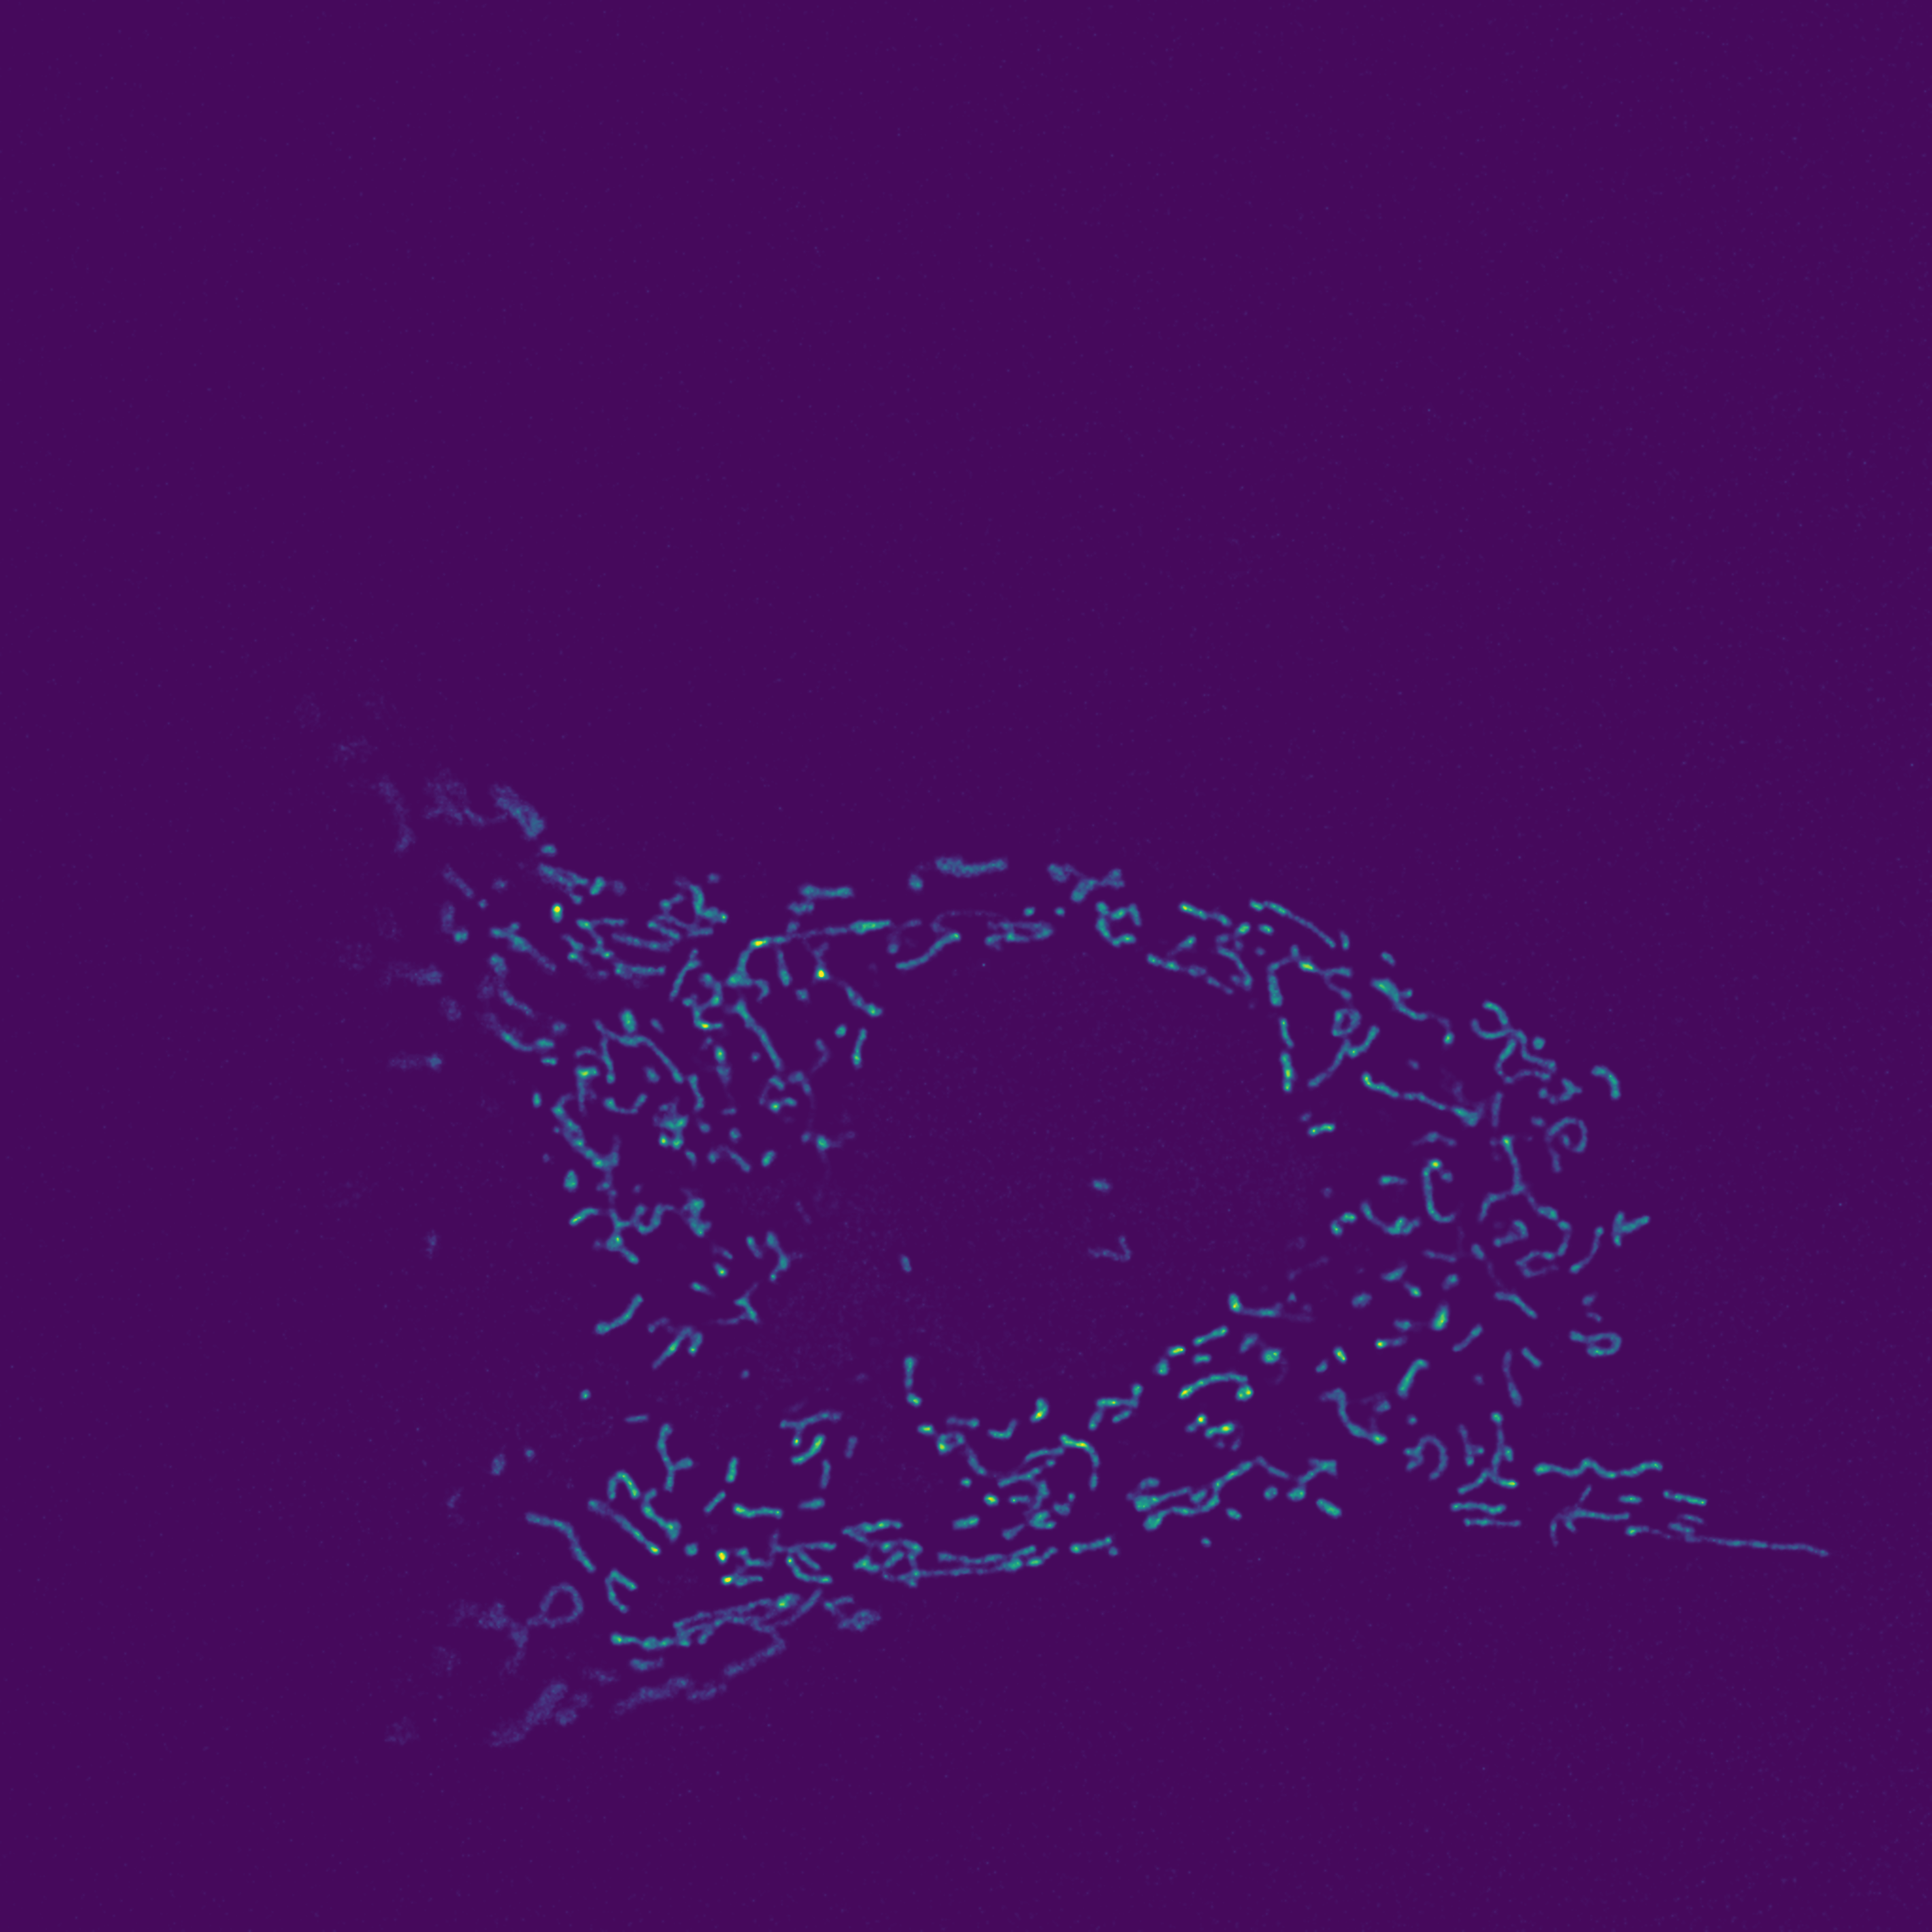
\includegraphics[width=0.49\textwidth]{figs/ch4figs/image_shortlisting/CCCP_1C=1T=0.png}}
	\subcaptionbox{Sample 2 (Lysosomes)}{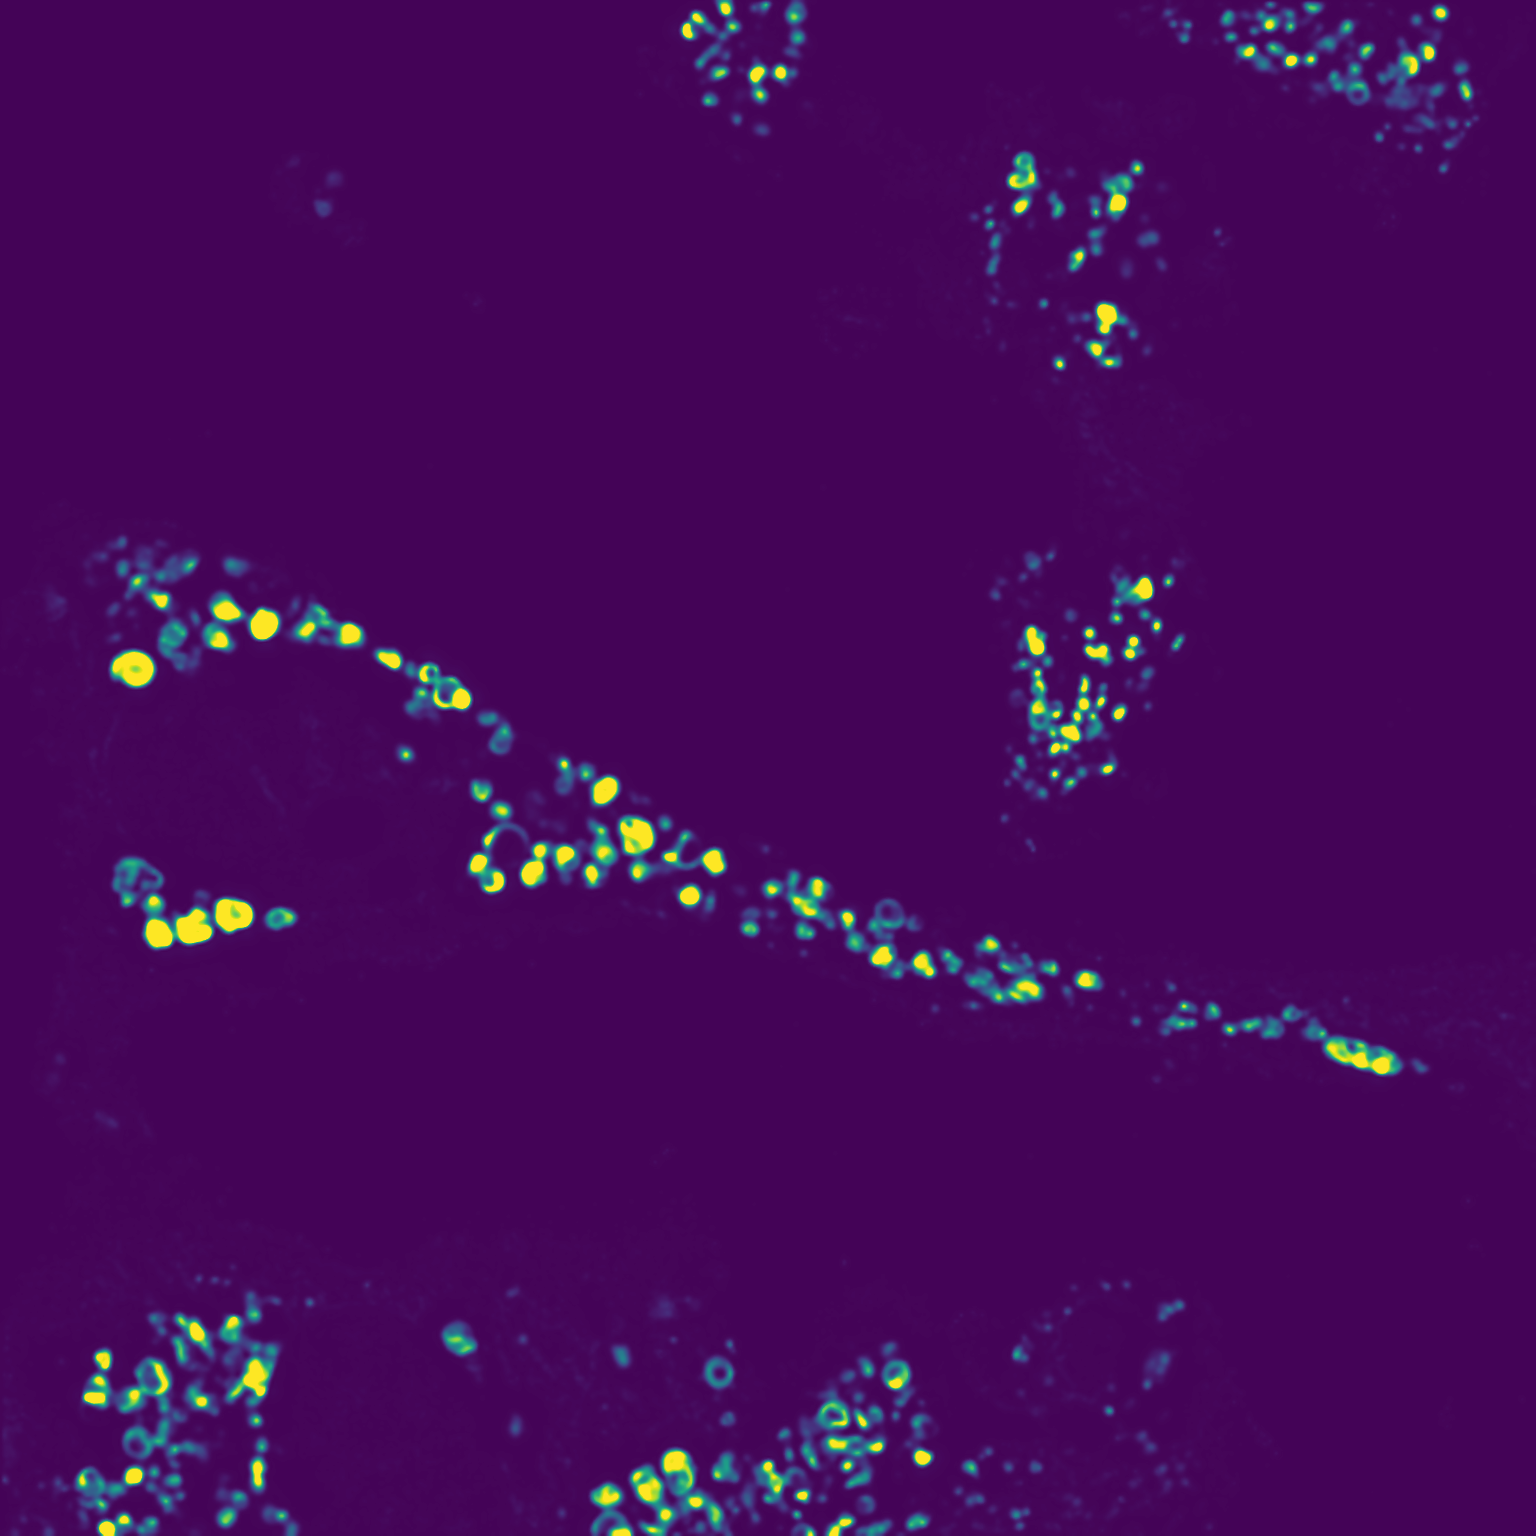
\includegraphics[width=0.49\textwidth]{figs/ch4figs/image_shortlisting/HML_4C=0.png}}
	\subcaptionbox{Sample 3 (Lysosomes)}{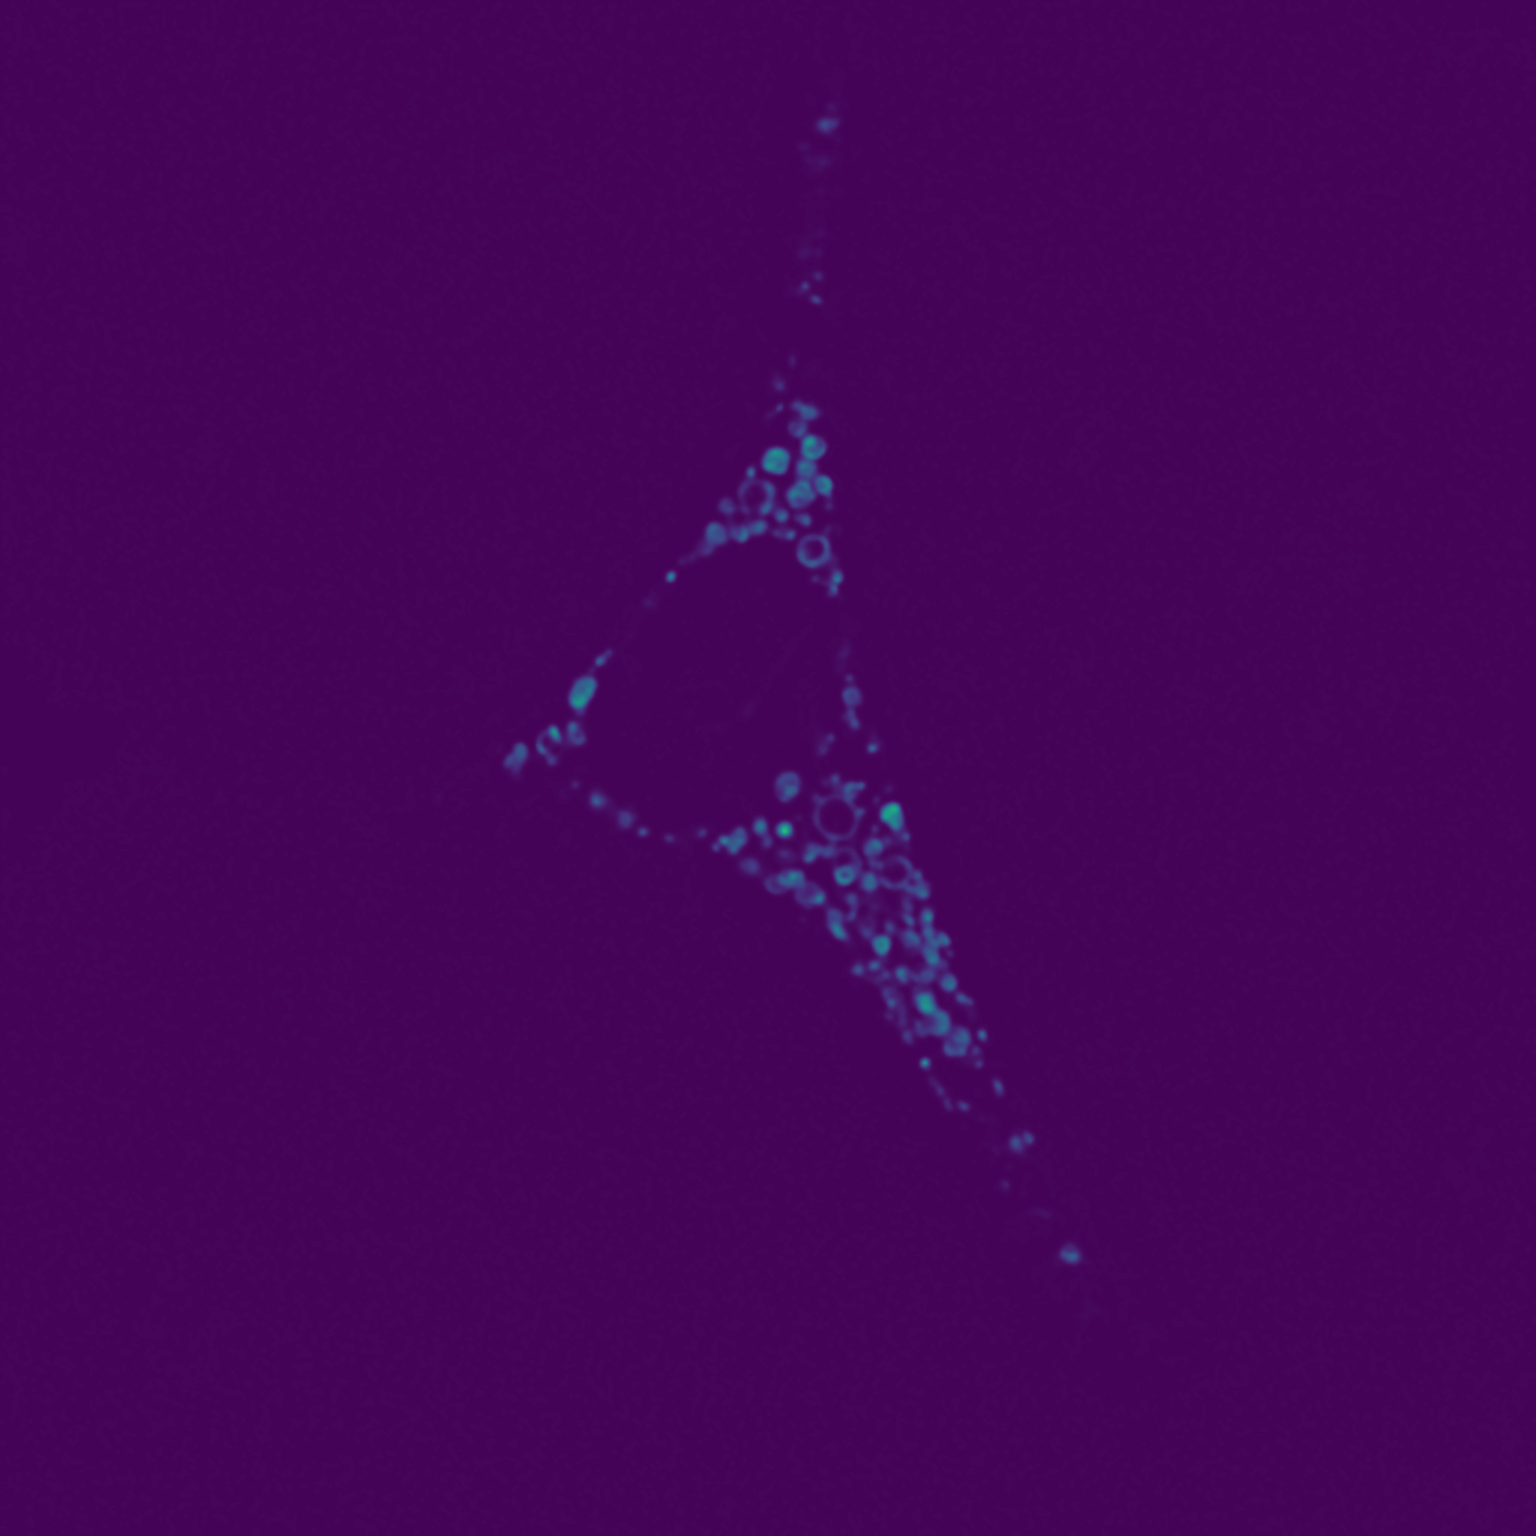
\includegraphics[width=0.49\textwidth]{figs/ch4figs/image_shortlisting/LML_3C=0.png}}
	\subcaptionbox{Sample 4 (Autophagosomes)}{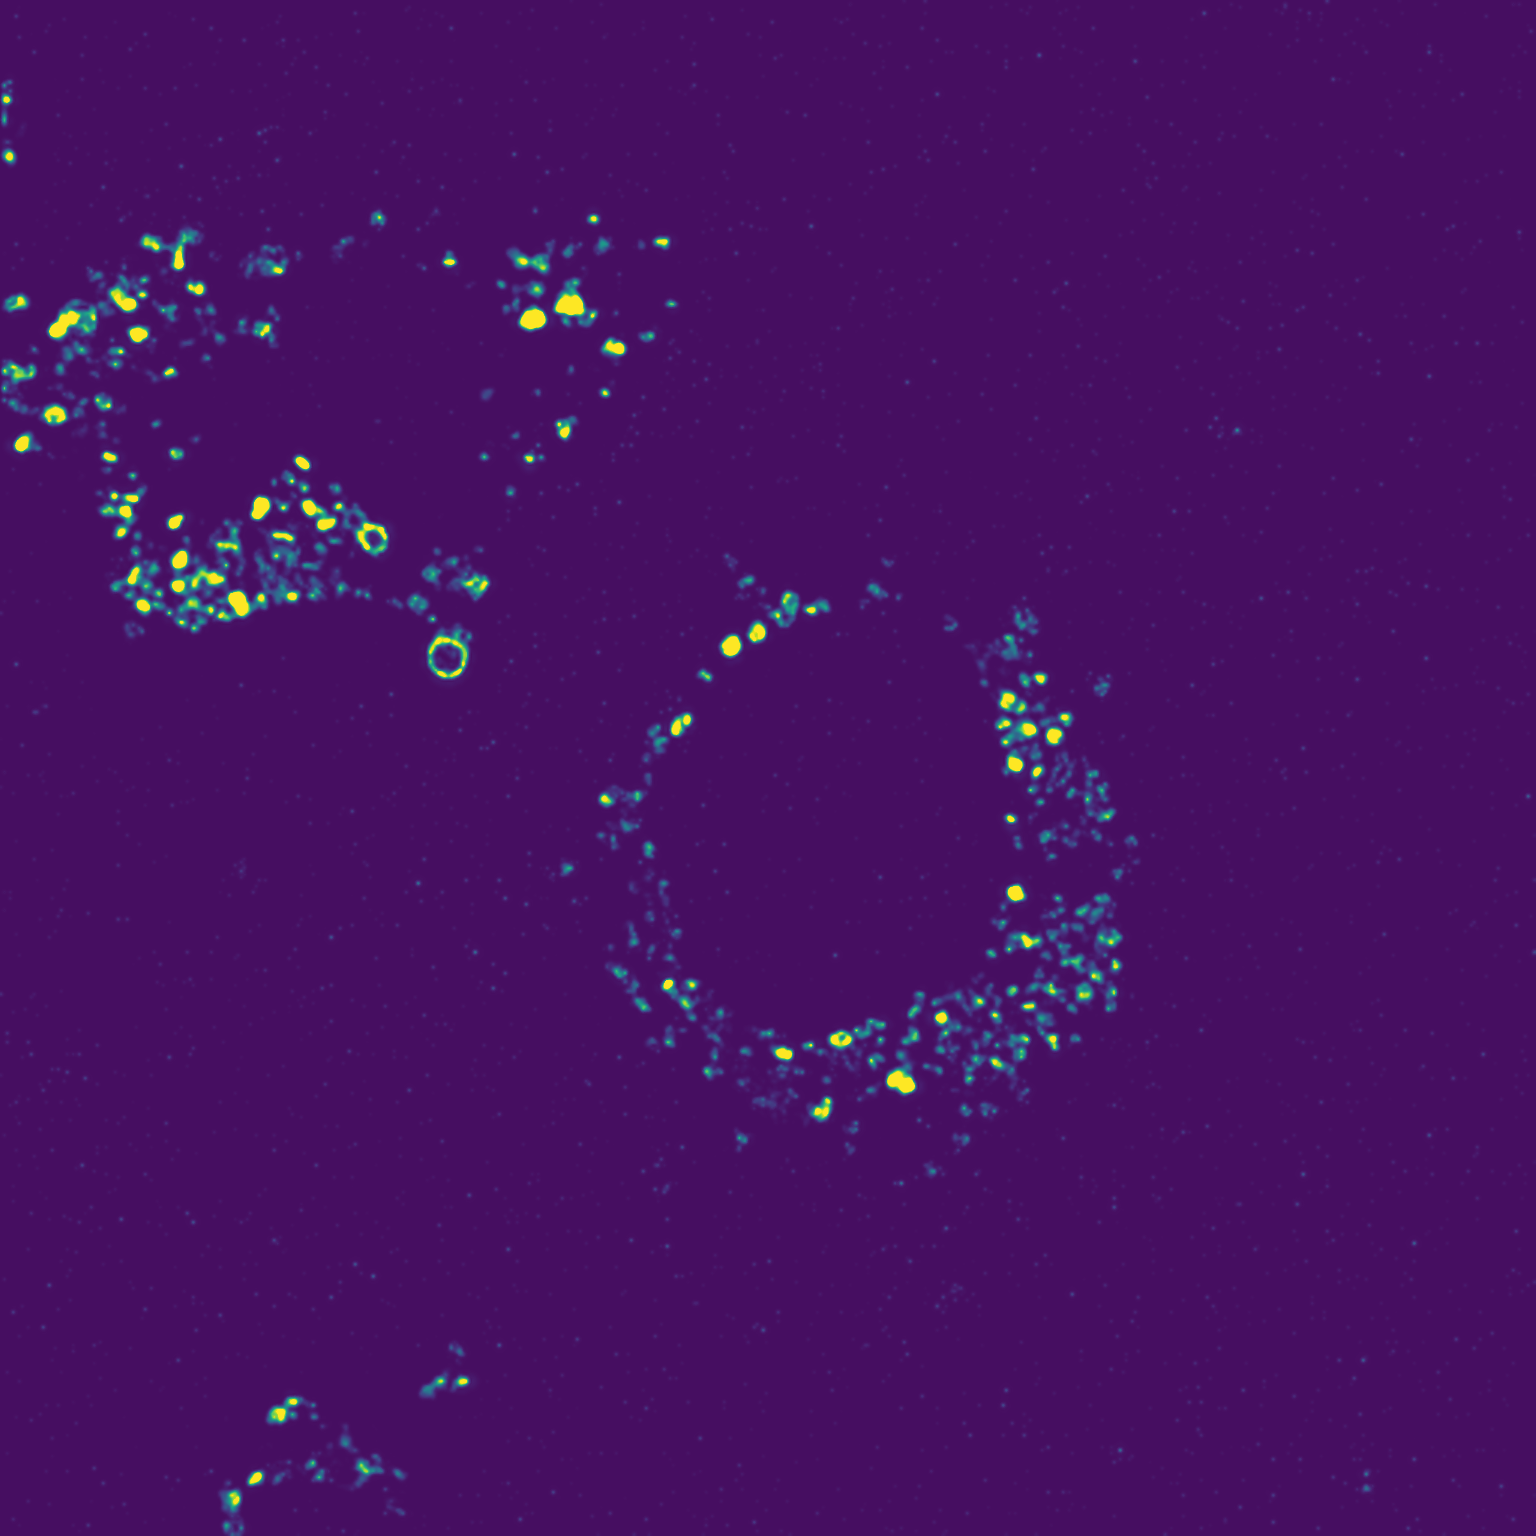
\includegraphics[width=0.49\textwidth]{figs/ch4figs/image_shortlisting/LML_4C=1.png}}
	\caption[Set of samples used to shortlist the threshold methods.]{Set of samples used to shortlist the threshold methods. The centre slice of the images, rounded down where necessary, of the images is shown.}
	\label{fig:shortlist_raw}
\end{figure}

\begin{figure}[ht!]
	\centering
	\subcaptionbox{Original sample image B\label{subfig:og_C_badthresh}}{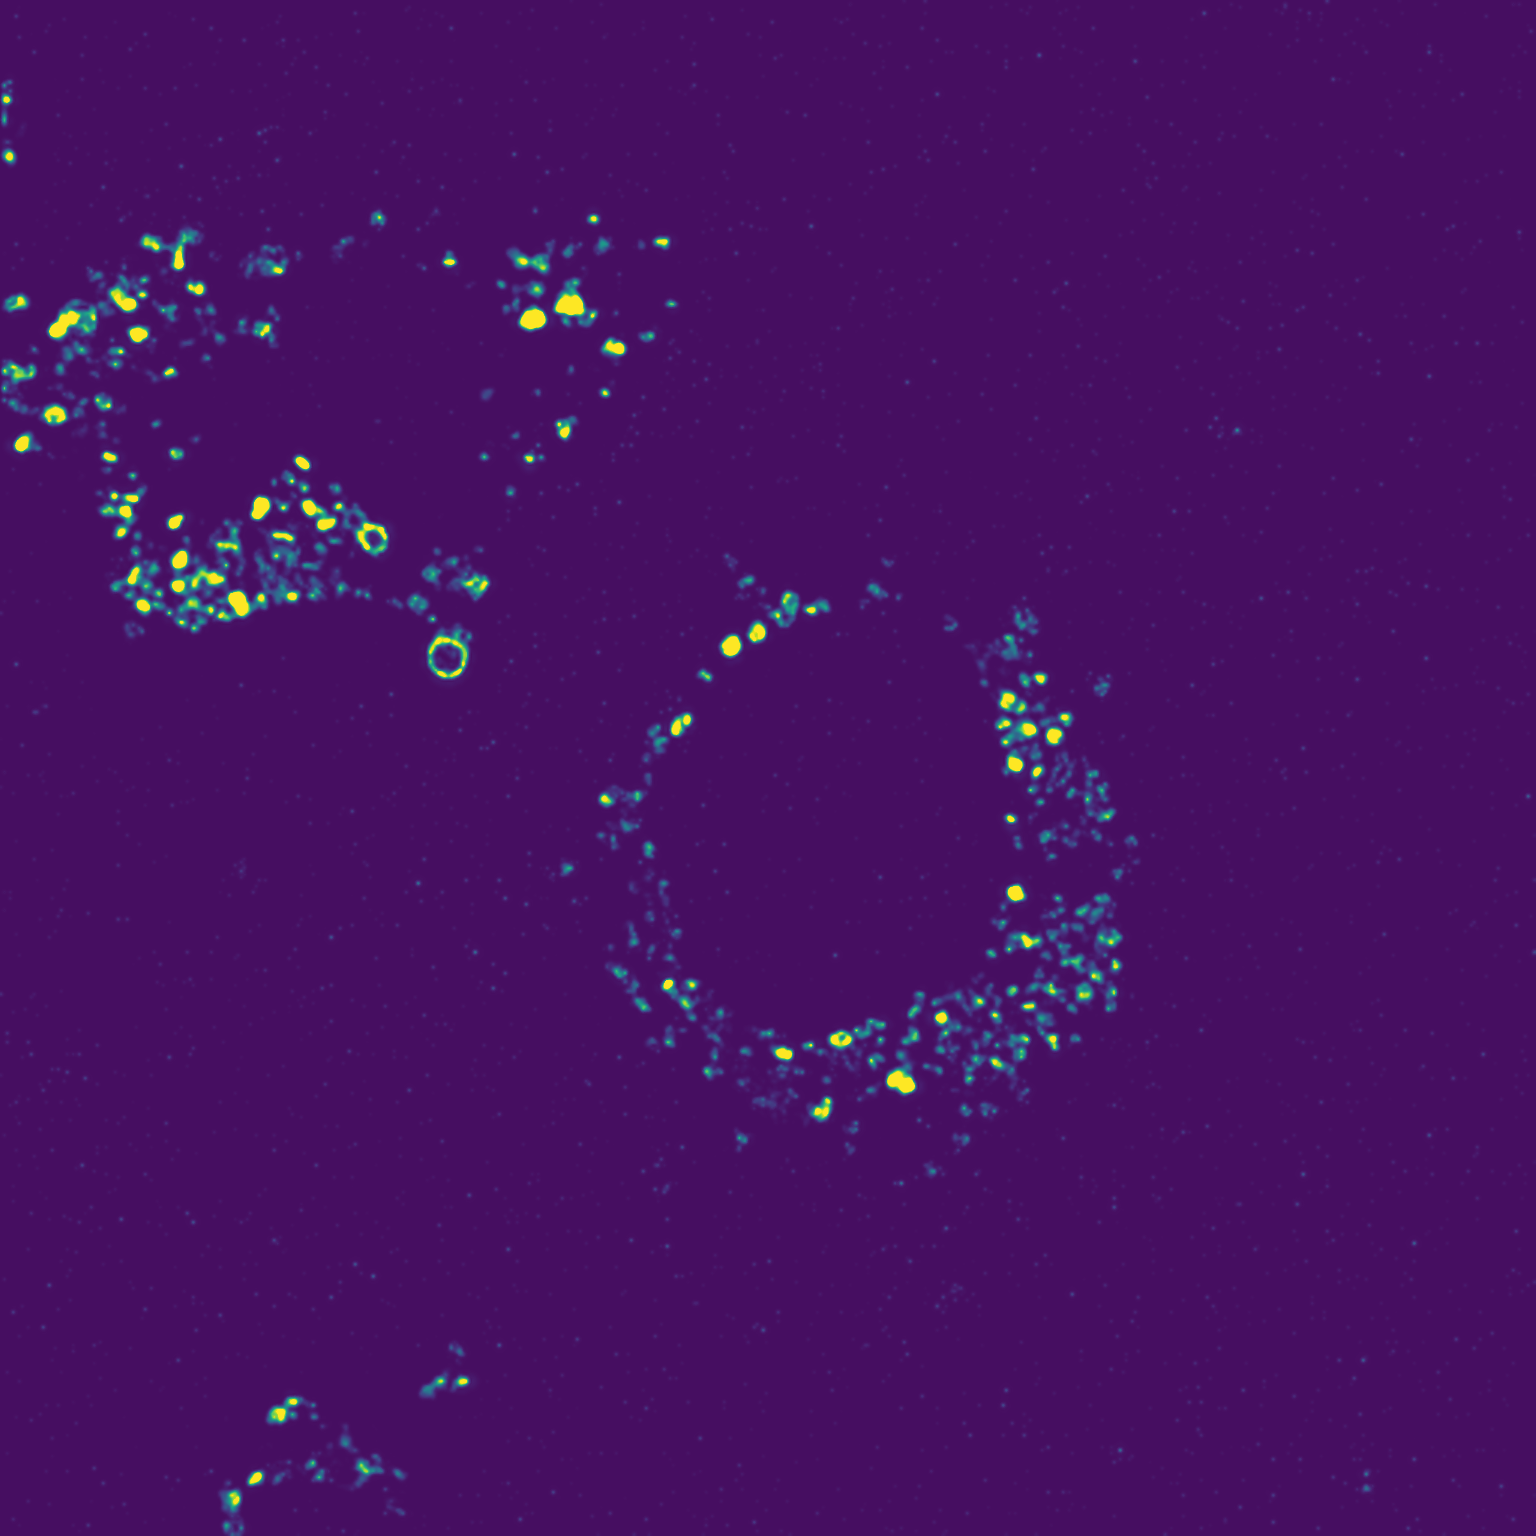
\includegraphics[width=0.45\textwidth]{figs/ch4figs/image_shortlisting/LML_4C=1.png}}
	\subcaptionbox{Original sample image C\label{subfig:og_B_badthresh}}{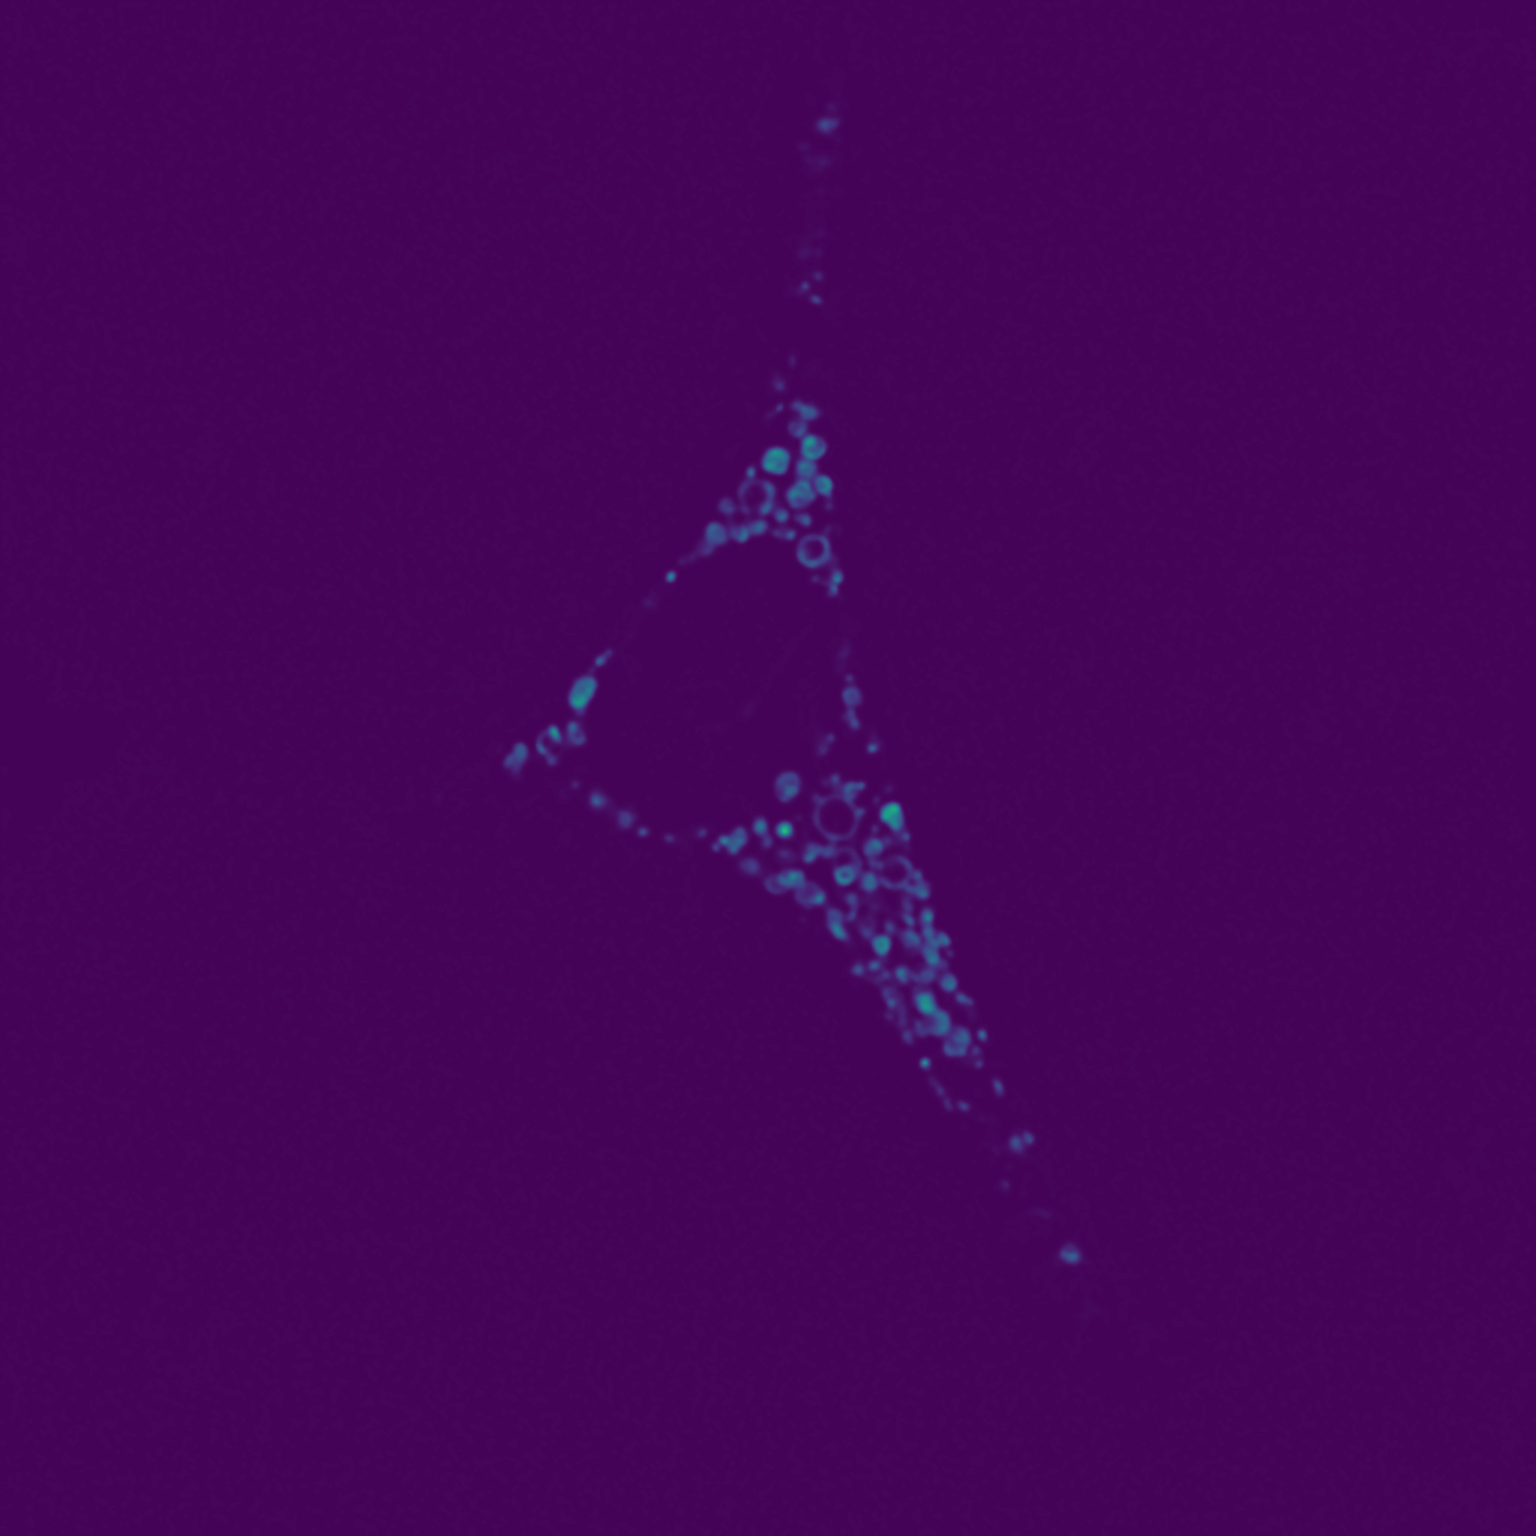
\includegraphics[width=0.45\textwidth]{figs/ch4figs/image_shortlisting/LML_3C=0.png}}
	\subcaptionbox{Mild background inclusion\label{subfig:mild_inclusion_C}}{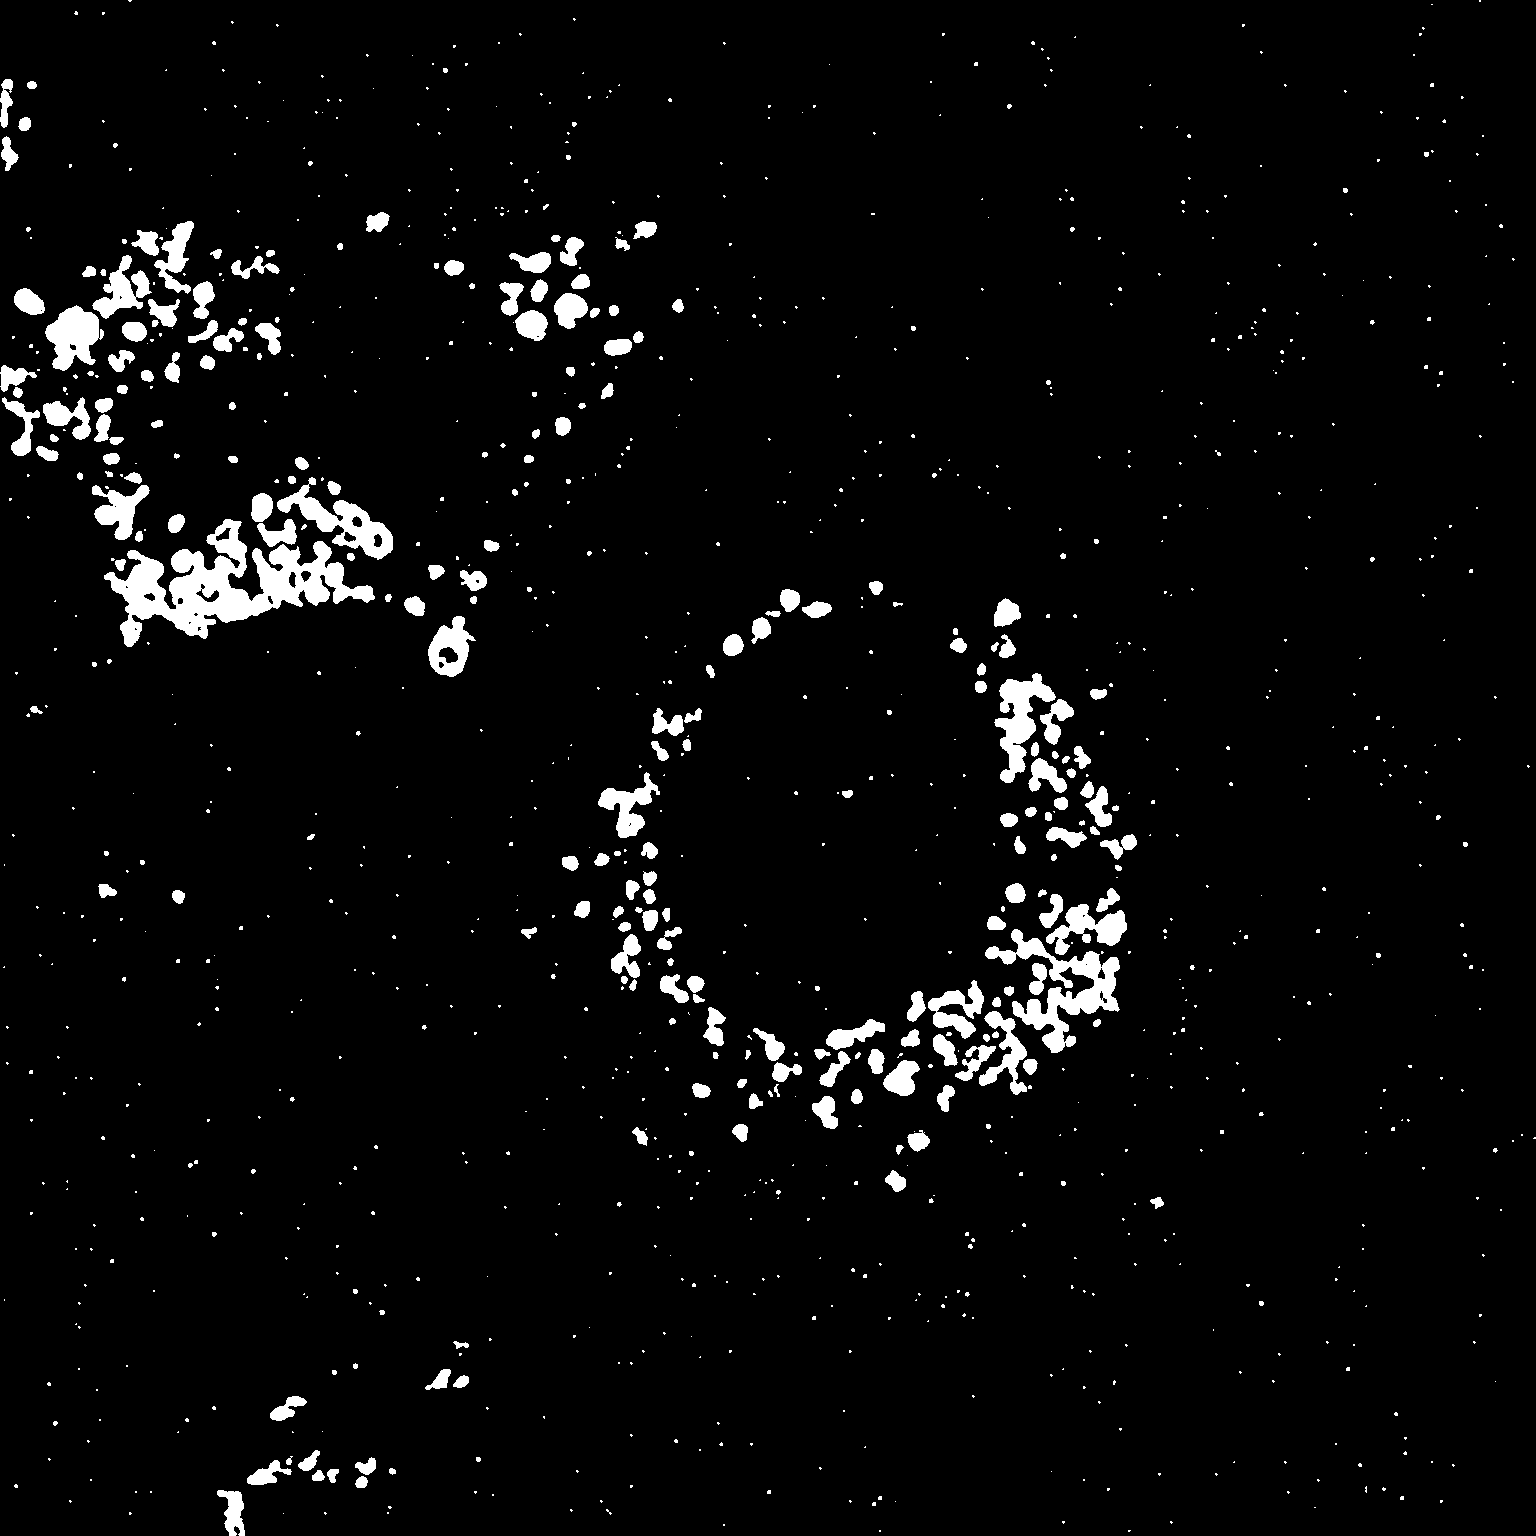
\includegraphics[width=0.45\textwidth]{figs/ch4figs/image_shortlisting/global/Li_LML_4C=1.png}}
	\subcaptionbox{Major background inclusion\label{subfig:major_inclusion_B}}{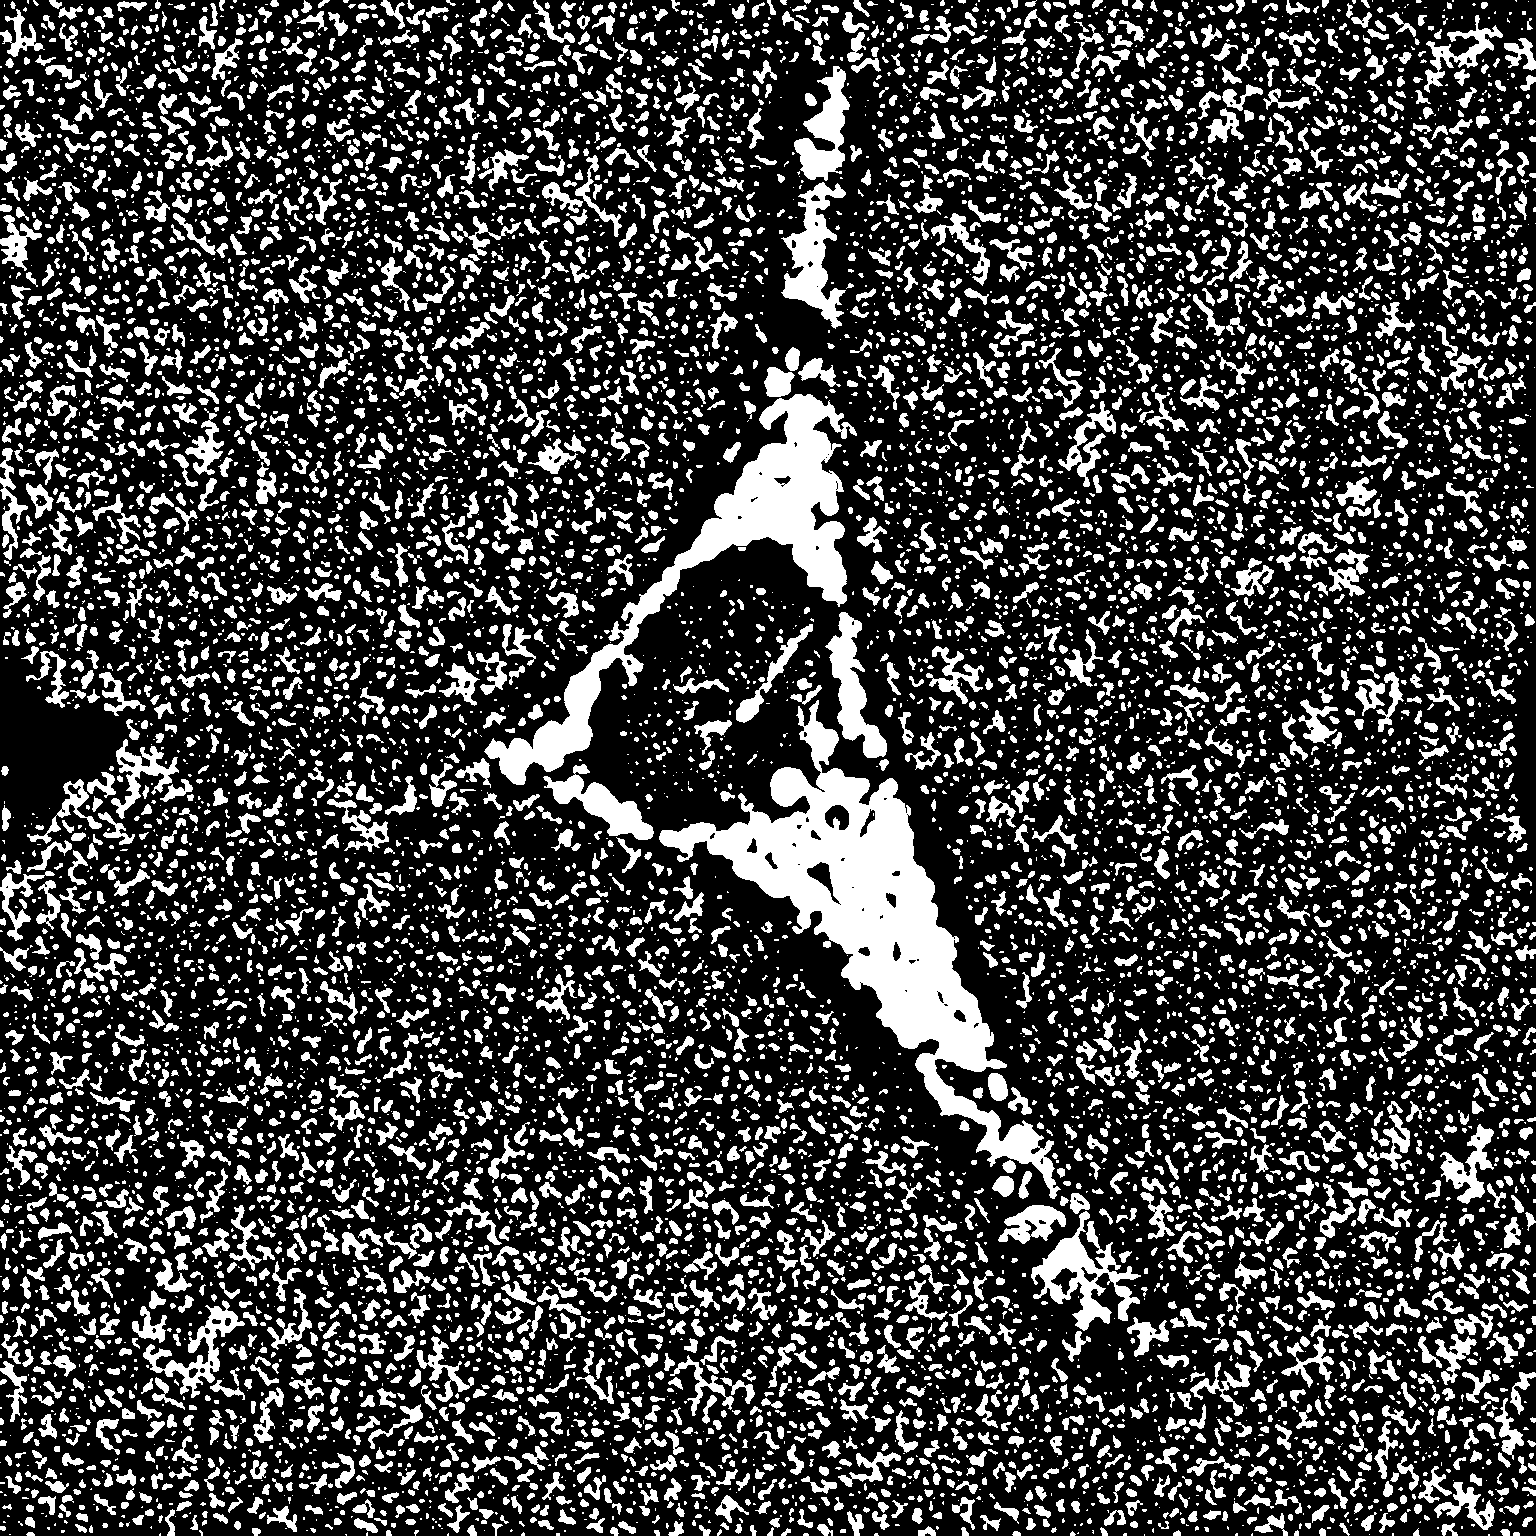
\includegraphics[width=0.45\textwidth]{figs/ch4figs/image_shortlisting/global/Mean_LML_3C=0.png}}
	\subcaptionbox{Mild foreground exclusion\label{subfig:mild_exclusion_C}}{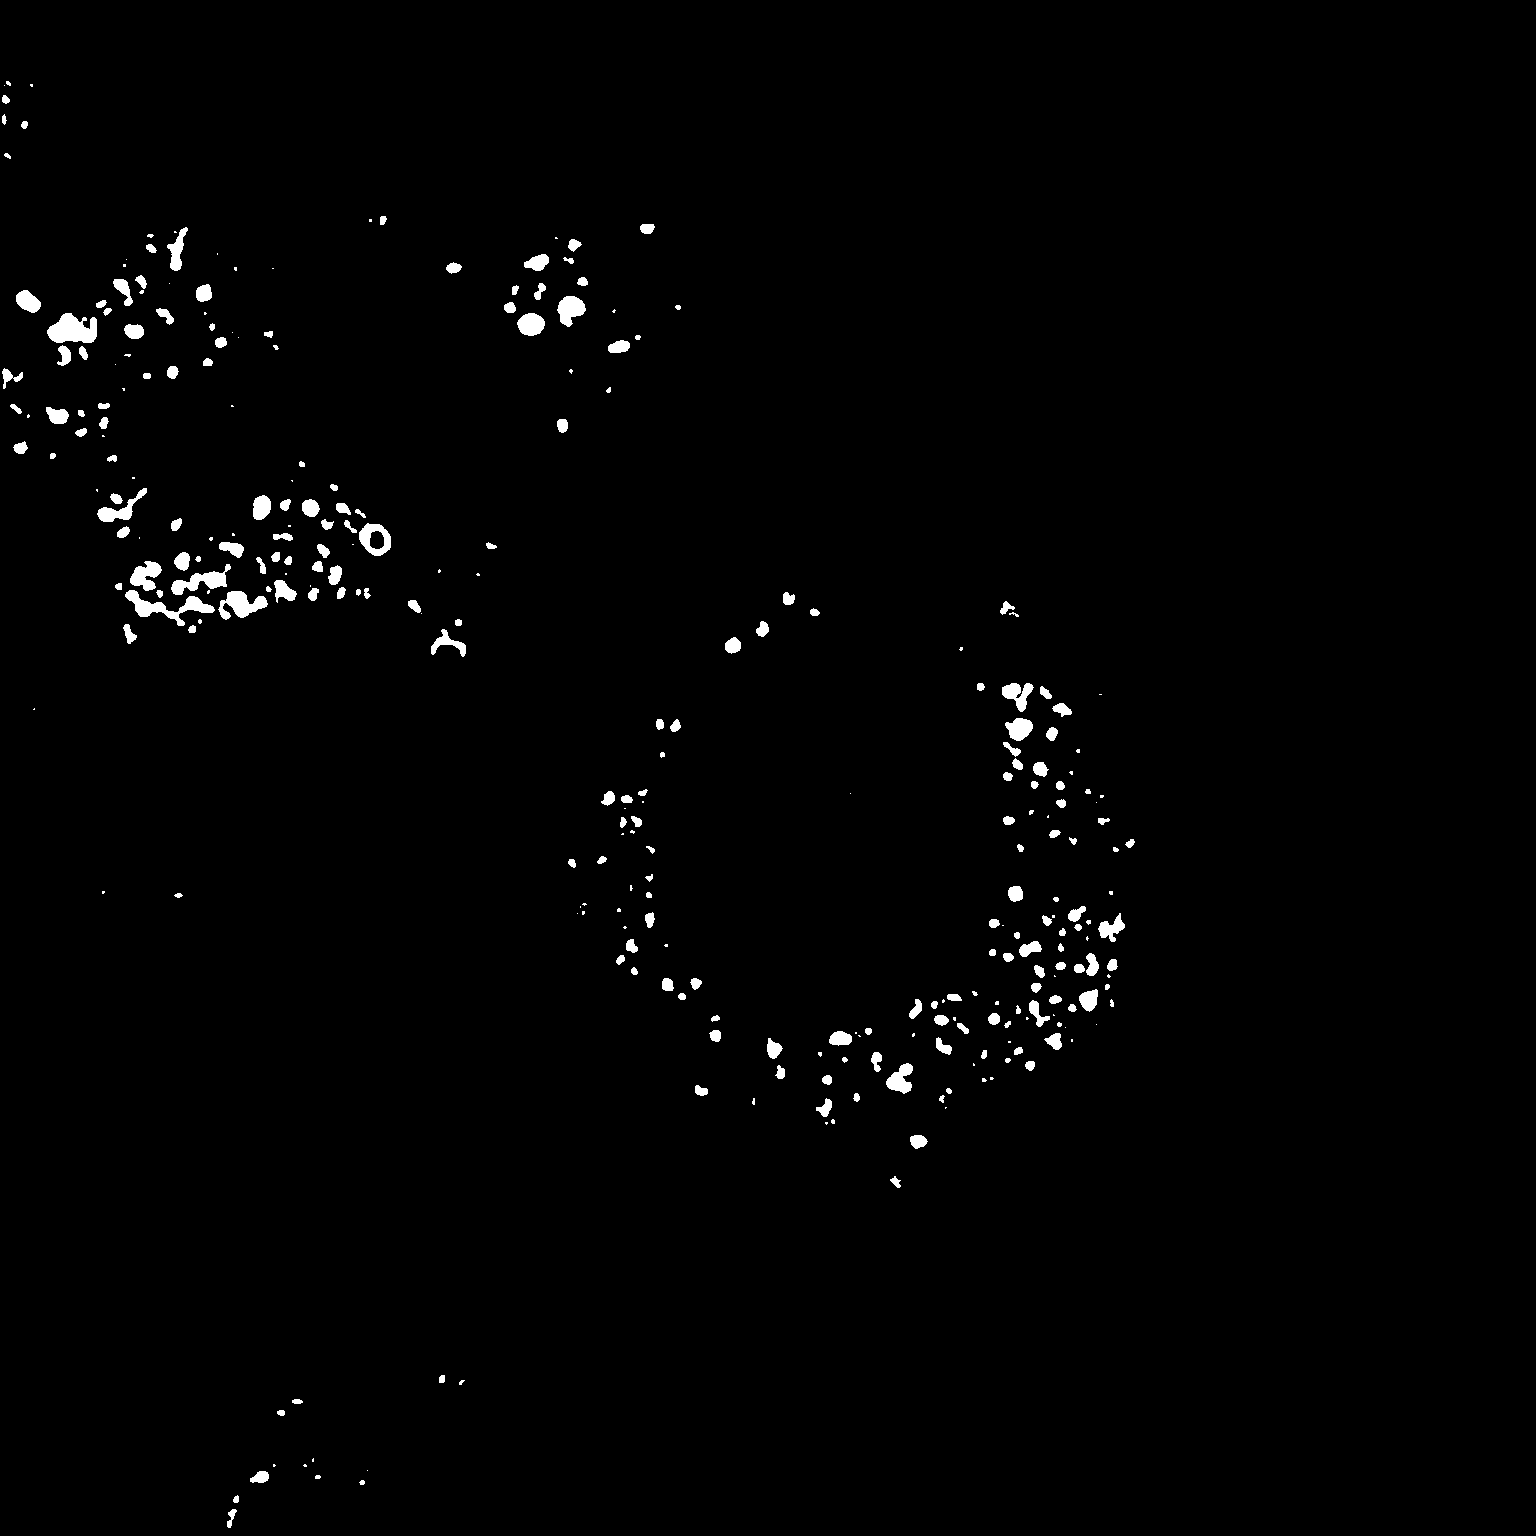
\includegraphics[width=0.45\textwidth]{figs/ch4figs/image_shortlisting/global/Moments_LML_4C=1.png}}
	\subcaptionbox{Major foreground exclusion\label{subfig:major_exclusion_B}}{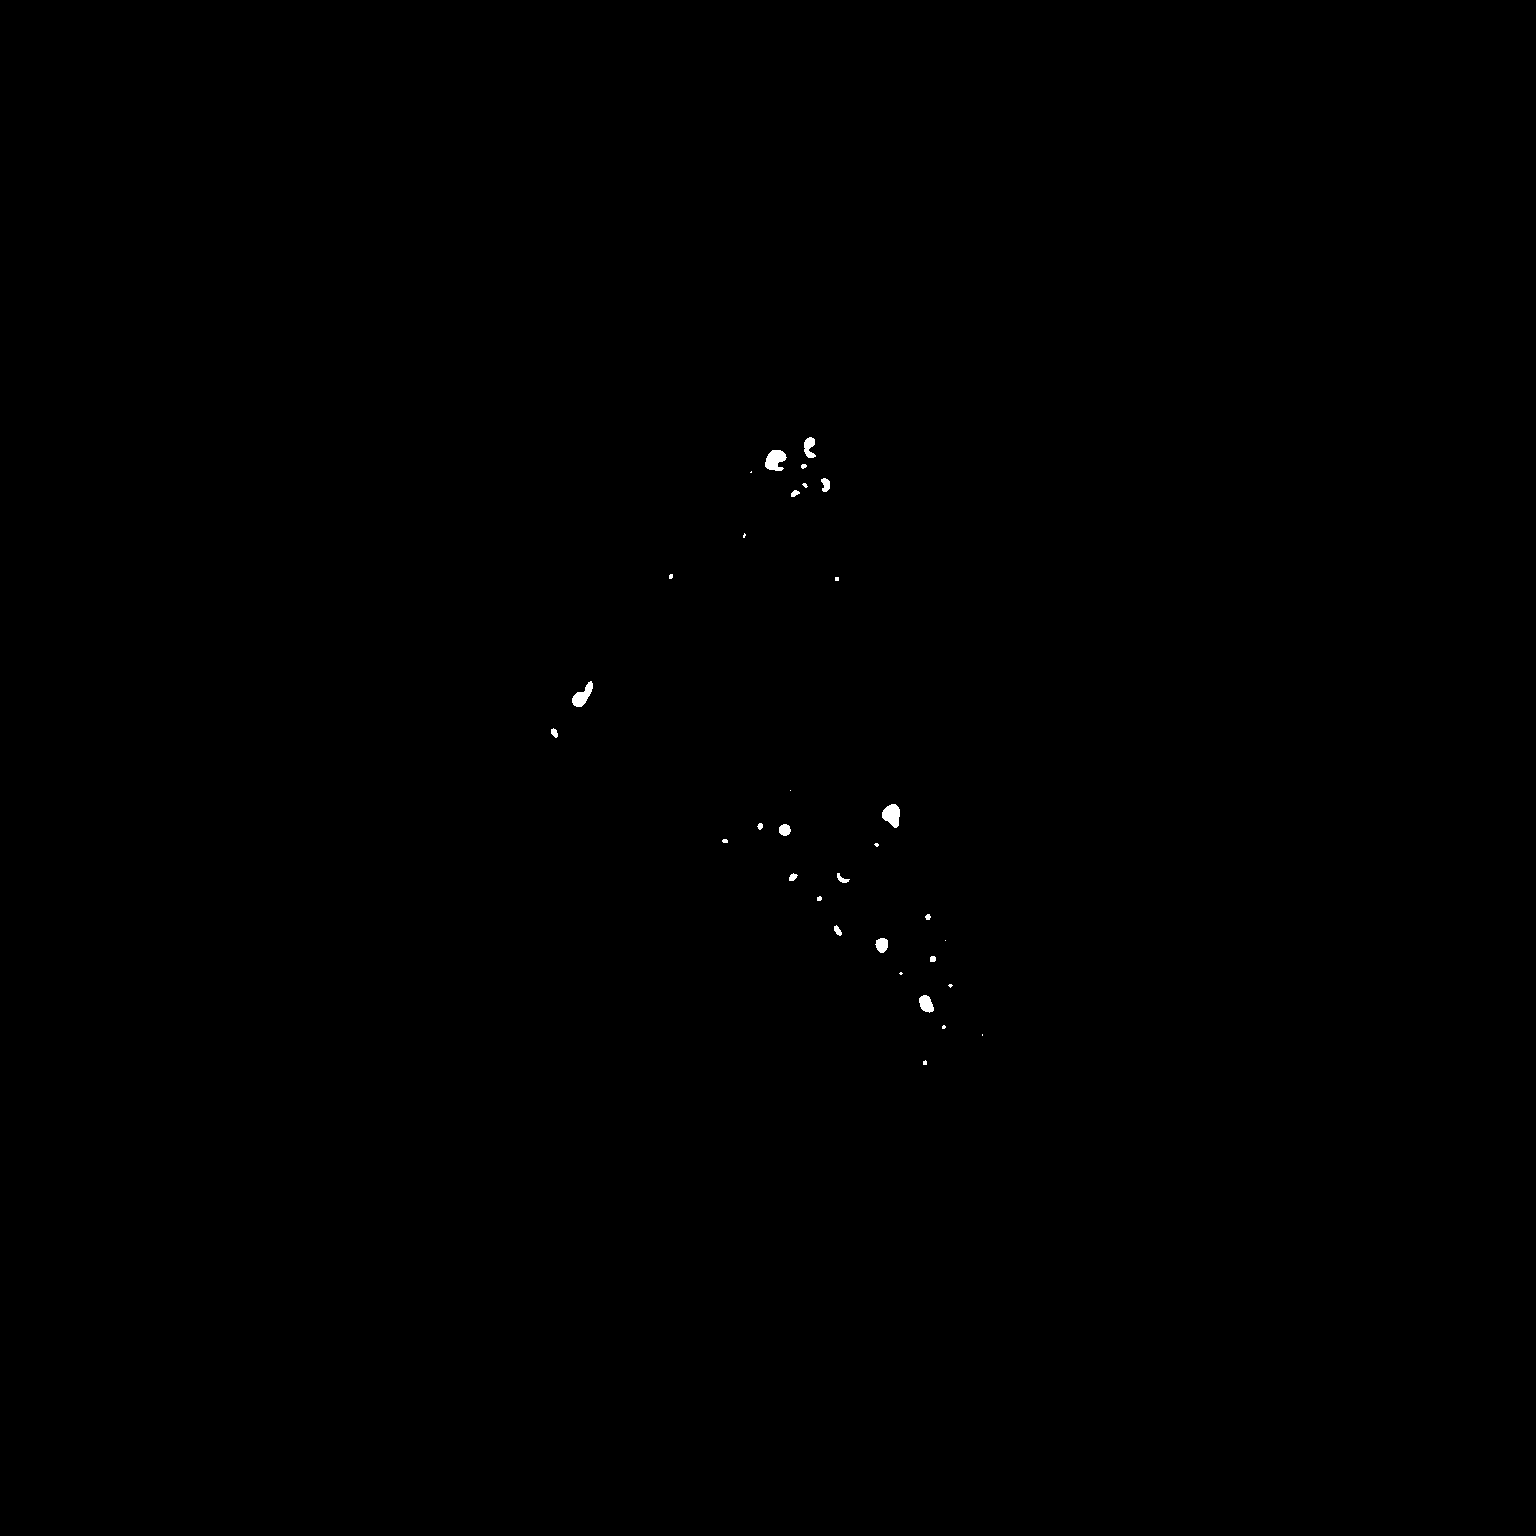
\includegraphics[width=0.45\textwidth]{figs/ch4figs/image_shortlisting/global/Intermodes_LML_3C=0.png}}
	\caption[Examples of both mild and major cases of background inclusion and foreground exclusion.]{Examples of both mild and major cases of background inclusion and of foreground exclusion. The sample images presented are Samples 2 and 3, shown in \ref{fig:shortlist_raw}, with (\subref{subfig:og_B_badthresh}), (\subref{subfig:major_inclusion_B}), and (\subref{subfig:major_exclusion_B}) representing the former and (\subref{subfig:og_C_badthresh}), (\subref{subfig:mild_inclusion_C}), and (\subref{subfig:mild_exclusion_C}) representing the latter.}
	\label{fig:bad_threshes_shortlist}
\end{figure}


\clearpage
\subsection{Global threshold shortlisting} 
A total of 16 global threshold methods, provided by the \textit{Auto Threshold} plugin, were tested across the shortlisting sample set:
\begin{multicols}{4}
	\begin{itemize}
		\setlength\itemsep{1mm}
		\item Huang
		\item Huang2
		\item Intermodes
		\item IsoData
		\item Li
		\item MaxEntropy
		\item Mean
		\item MinError(I)
		\item Minimum
		\item Moments
		\item Otsu
		\item Percentile
		\item RenyiEntropy
		\item Shanbhag
		\item Triangle
		\item Yen
	\end{itemize}
\end{multicols}
\paragraph{Findings:} Of the global thresholding methods explored, the Huang2, IsoData, Li, MaxEntropy, Moments, Otsu, RenyiEntropy, Triangle, and Yen methods were deemed viable for further evaluation due to the presence of mostly mild foreground exclusion and background inclusion and it is nuanced whether mild cases are detrimental and, if so, to what degree. While evaluating the severity of these is subjective, save for the extreme cases, it was observed that the viable methods only present at most two mild cases per method while only the Triangle method presents a singular instance of more severe background inclusion although this is still not comparable to the major case illustrated in Figure \ref{fig:bad_threshes_shortlist} (\subref{subfig:major_inclusion_B}). While this does not imply that the performance of these methods will be the same for evaluations involving different image data sets, it does flag methods expressing major foreground exclusion and background inclusion behaviours. Major occurrences of background inclusion can be seen in methods Huang (Figure \ref{append-fig:huang_short}), Mean (Figure \ref{append-fig:Mean_short}), MinError(I) (Figure \ref{append-fig:MinError_short}), and Percentile (Figure \ref{append-fig:Percentile_short}) while major occurrences of foreground exclusion can be seen in methods Intermodes (Figure \ref{append-fig:Intermodes_short}), Minimum (Figure \ref{append-fig:Minimum_short}), and Shanbhag (Figure \ref{append-fig:Shanbhag_short}). Due to this, these methods have been deemed not worth further exploration in this study due to this poor performance and the showcasing of a singular case of either major foreground exclusion or background inclusion, dependent on the method, is shown in Figure \ref{fig:bad_global_subset} for the methods not deemed worth further exploration. 

\begin{figure}[ht!]
	\centering
	\subcaptionbox{Intermodes applied to Sample 4}{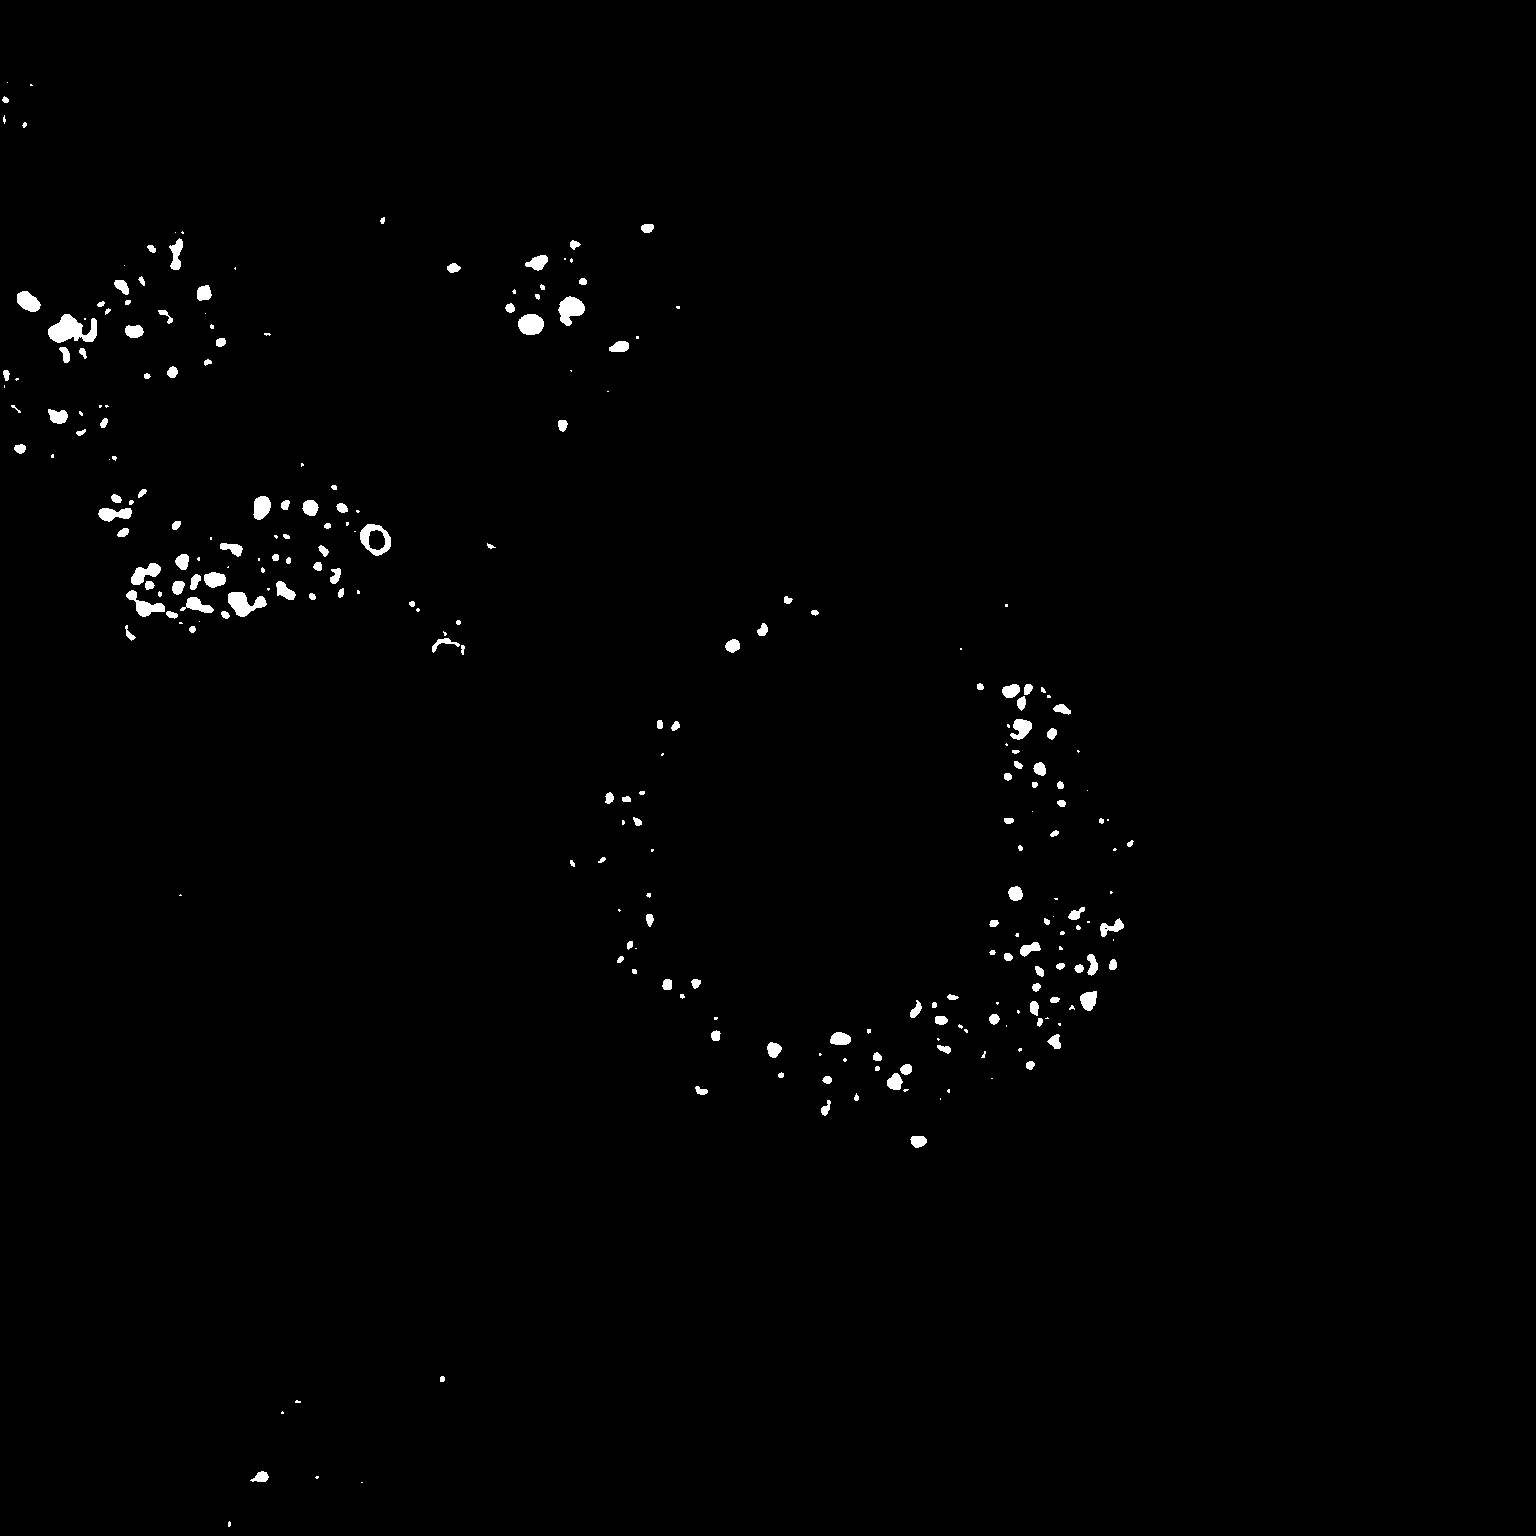
\includegraphics[width=0.24\textwidth]{figs/ch4figs/image_shortlisting/global/Intermodes_LML_4C=1.png}}
	\subcaptionbox{Minimum applied to Sample 1}{
\includegraphics[width=0.24\textwidth]{figs/ch4figs/image_shortlisting/global/Minimum_CCCP_1C=1T=0.png}}
	\subcaptionbox{Shanbhag applied to Sample 4}{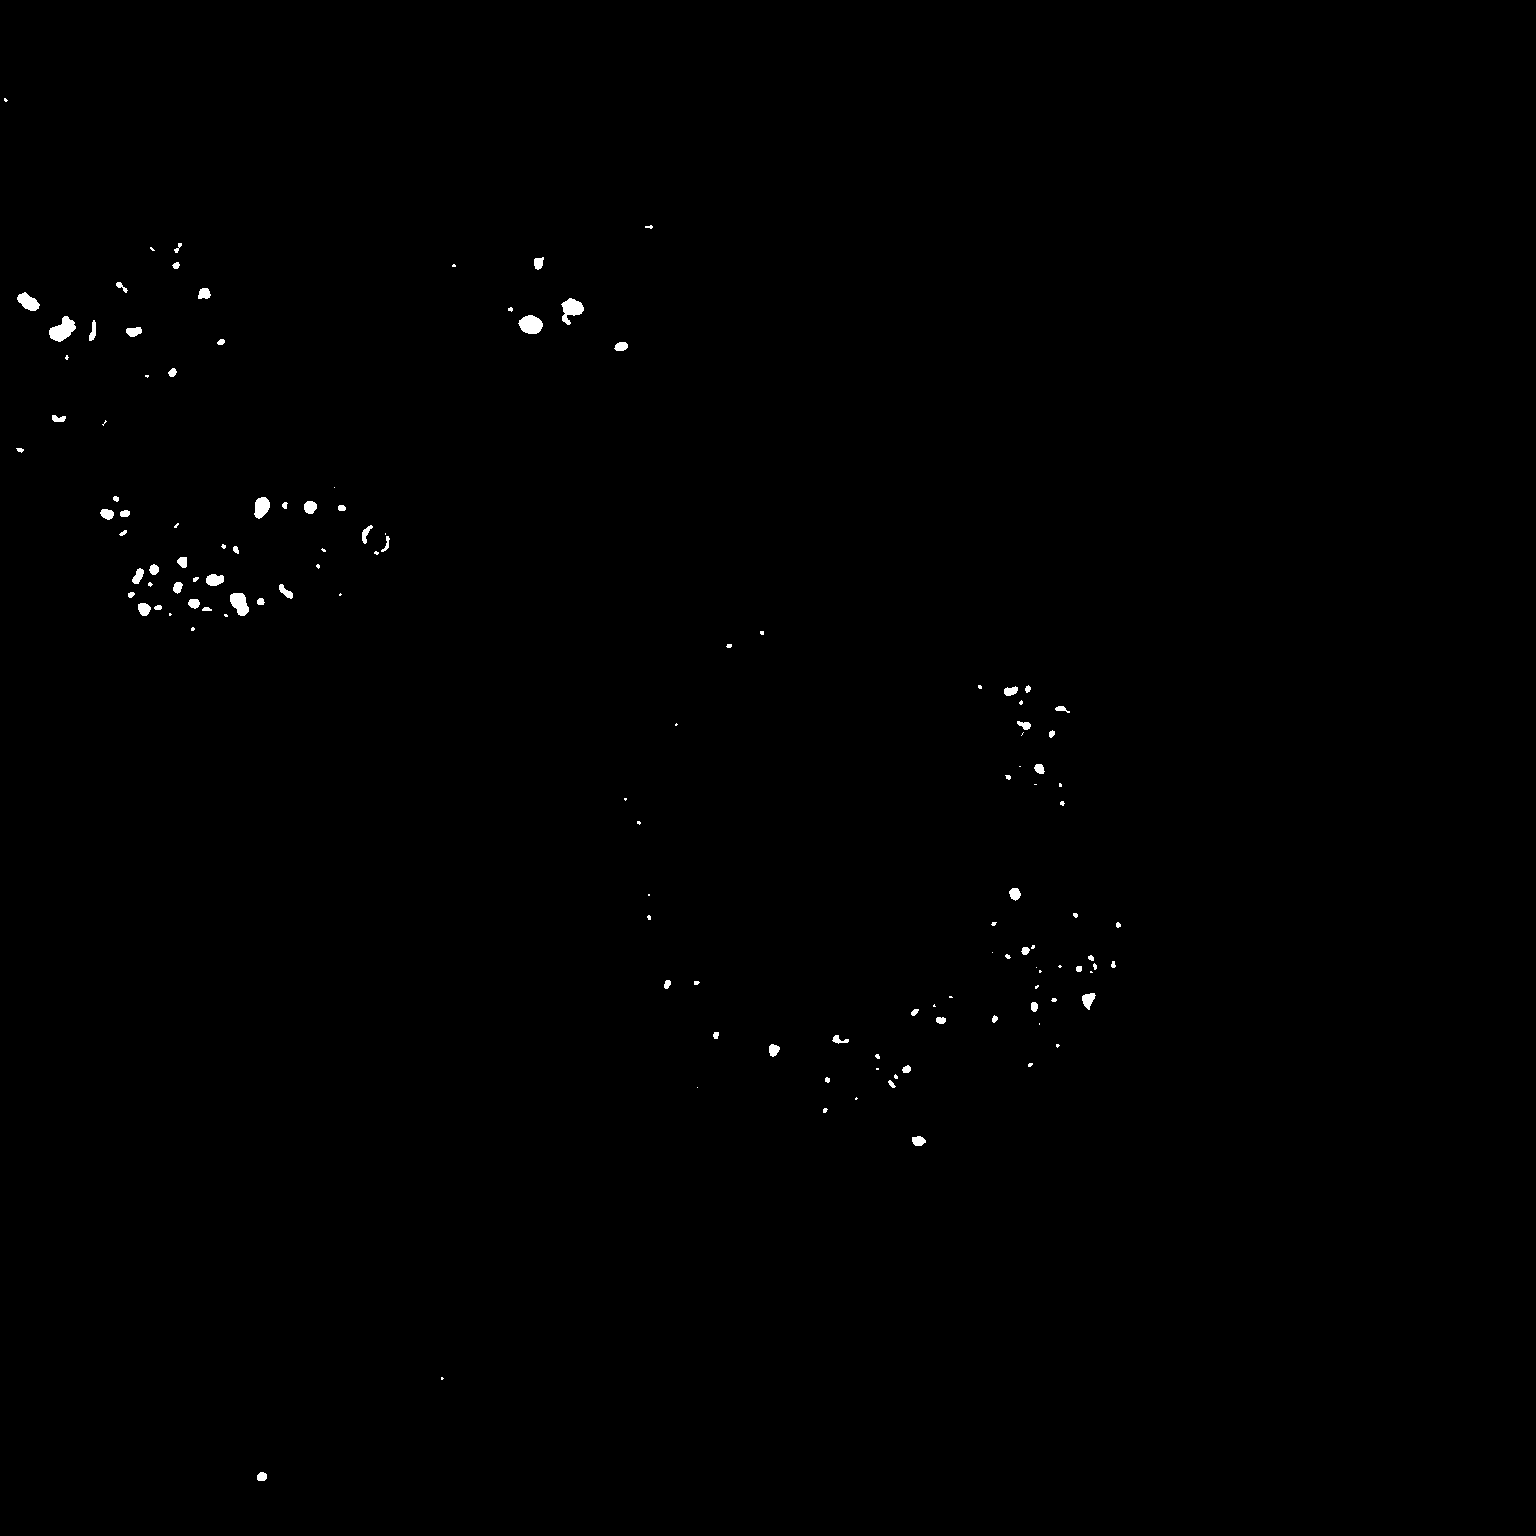
\includegraphics[width=0.24\textwidth]{figs/ch4figs/image_shortlisting/global/Shanbhag_LML_4C=1.png}}
	\subcaptionbox{MinError(I) applied to Sample 3}{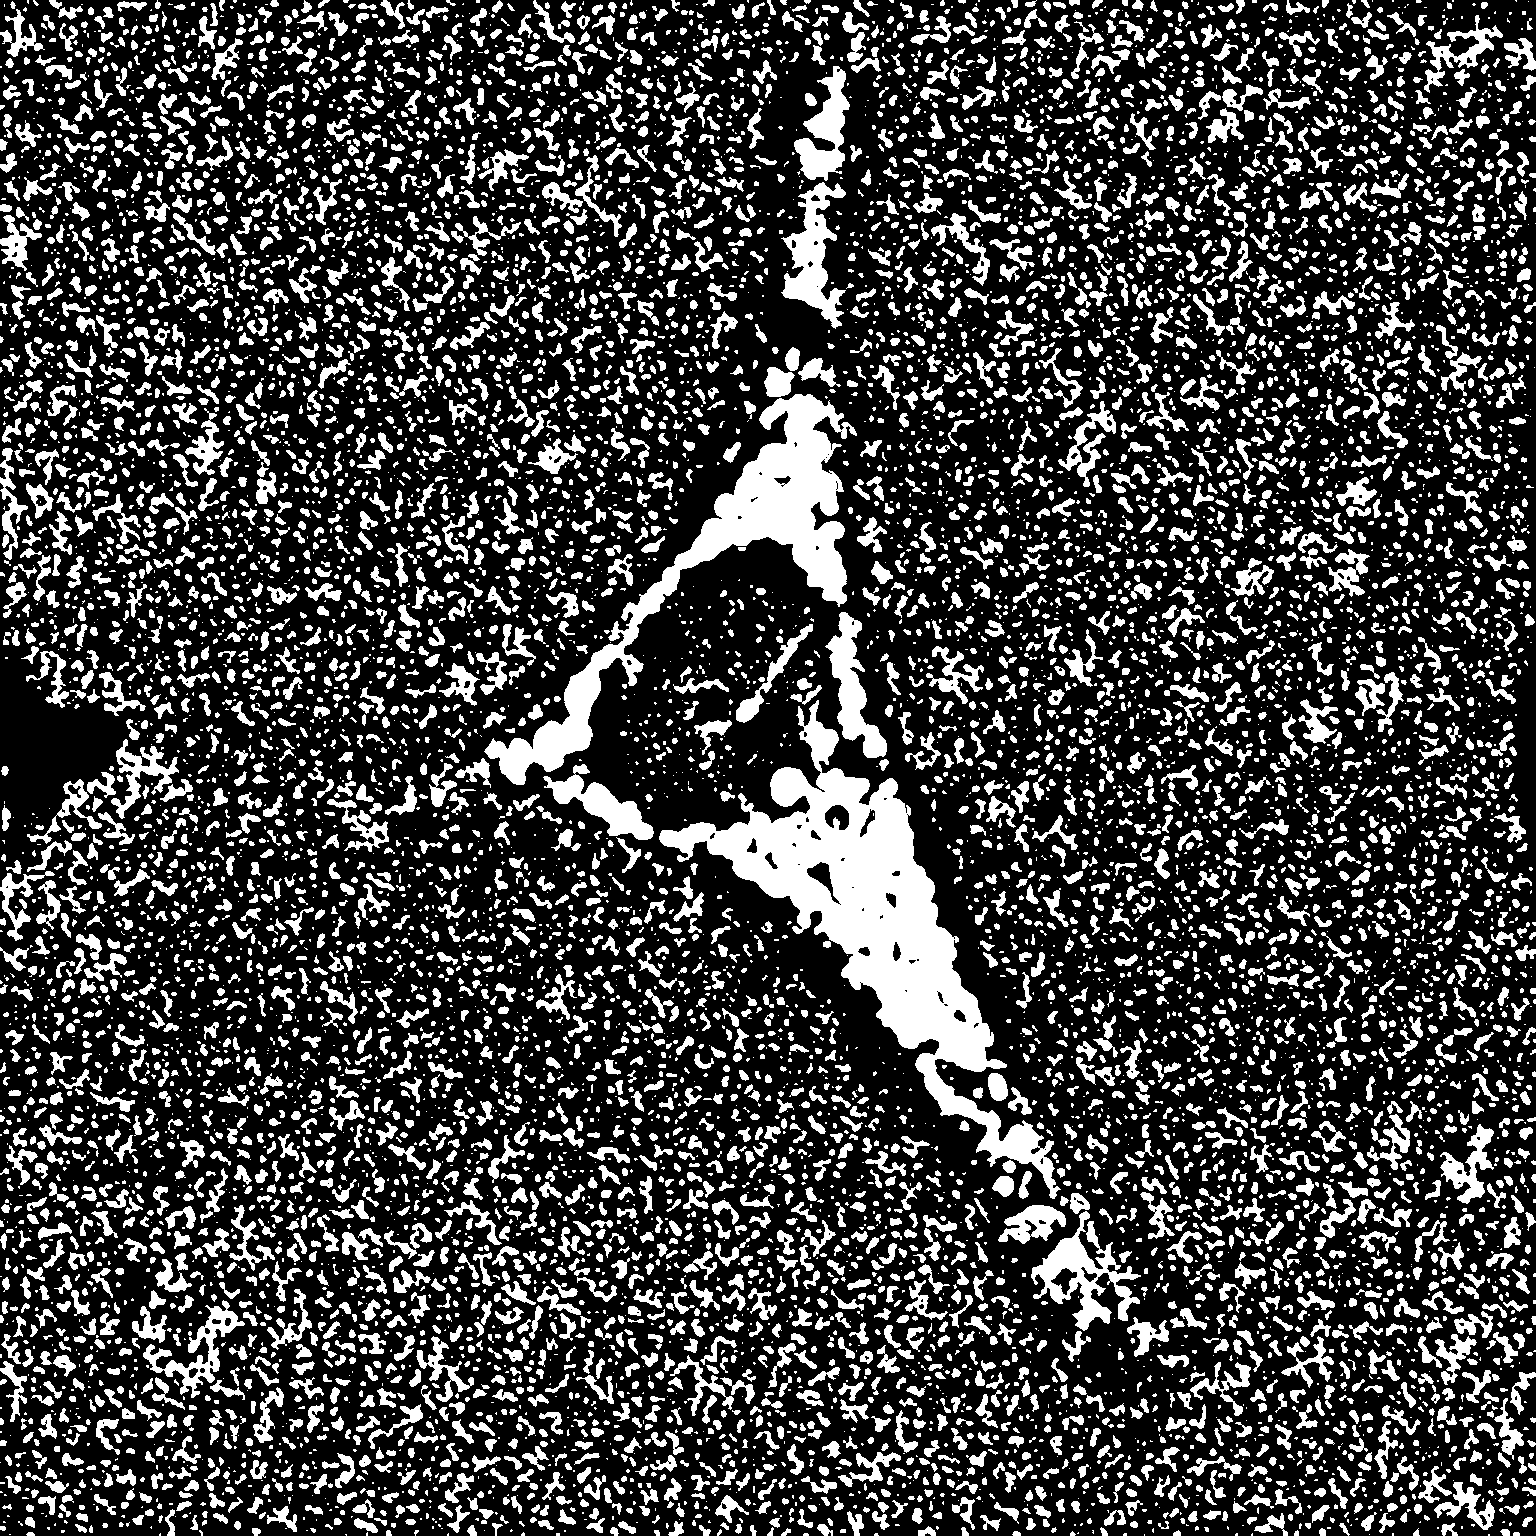
\includegraphics[width=0.24\textwidth]{figs/ch4figs/image_shortlisting/global/MinError(I)_LML_3C=0.png}}
	\subcaptionbox{Percentile applied to Sample 2}{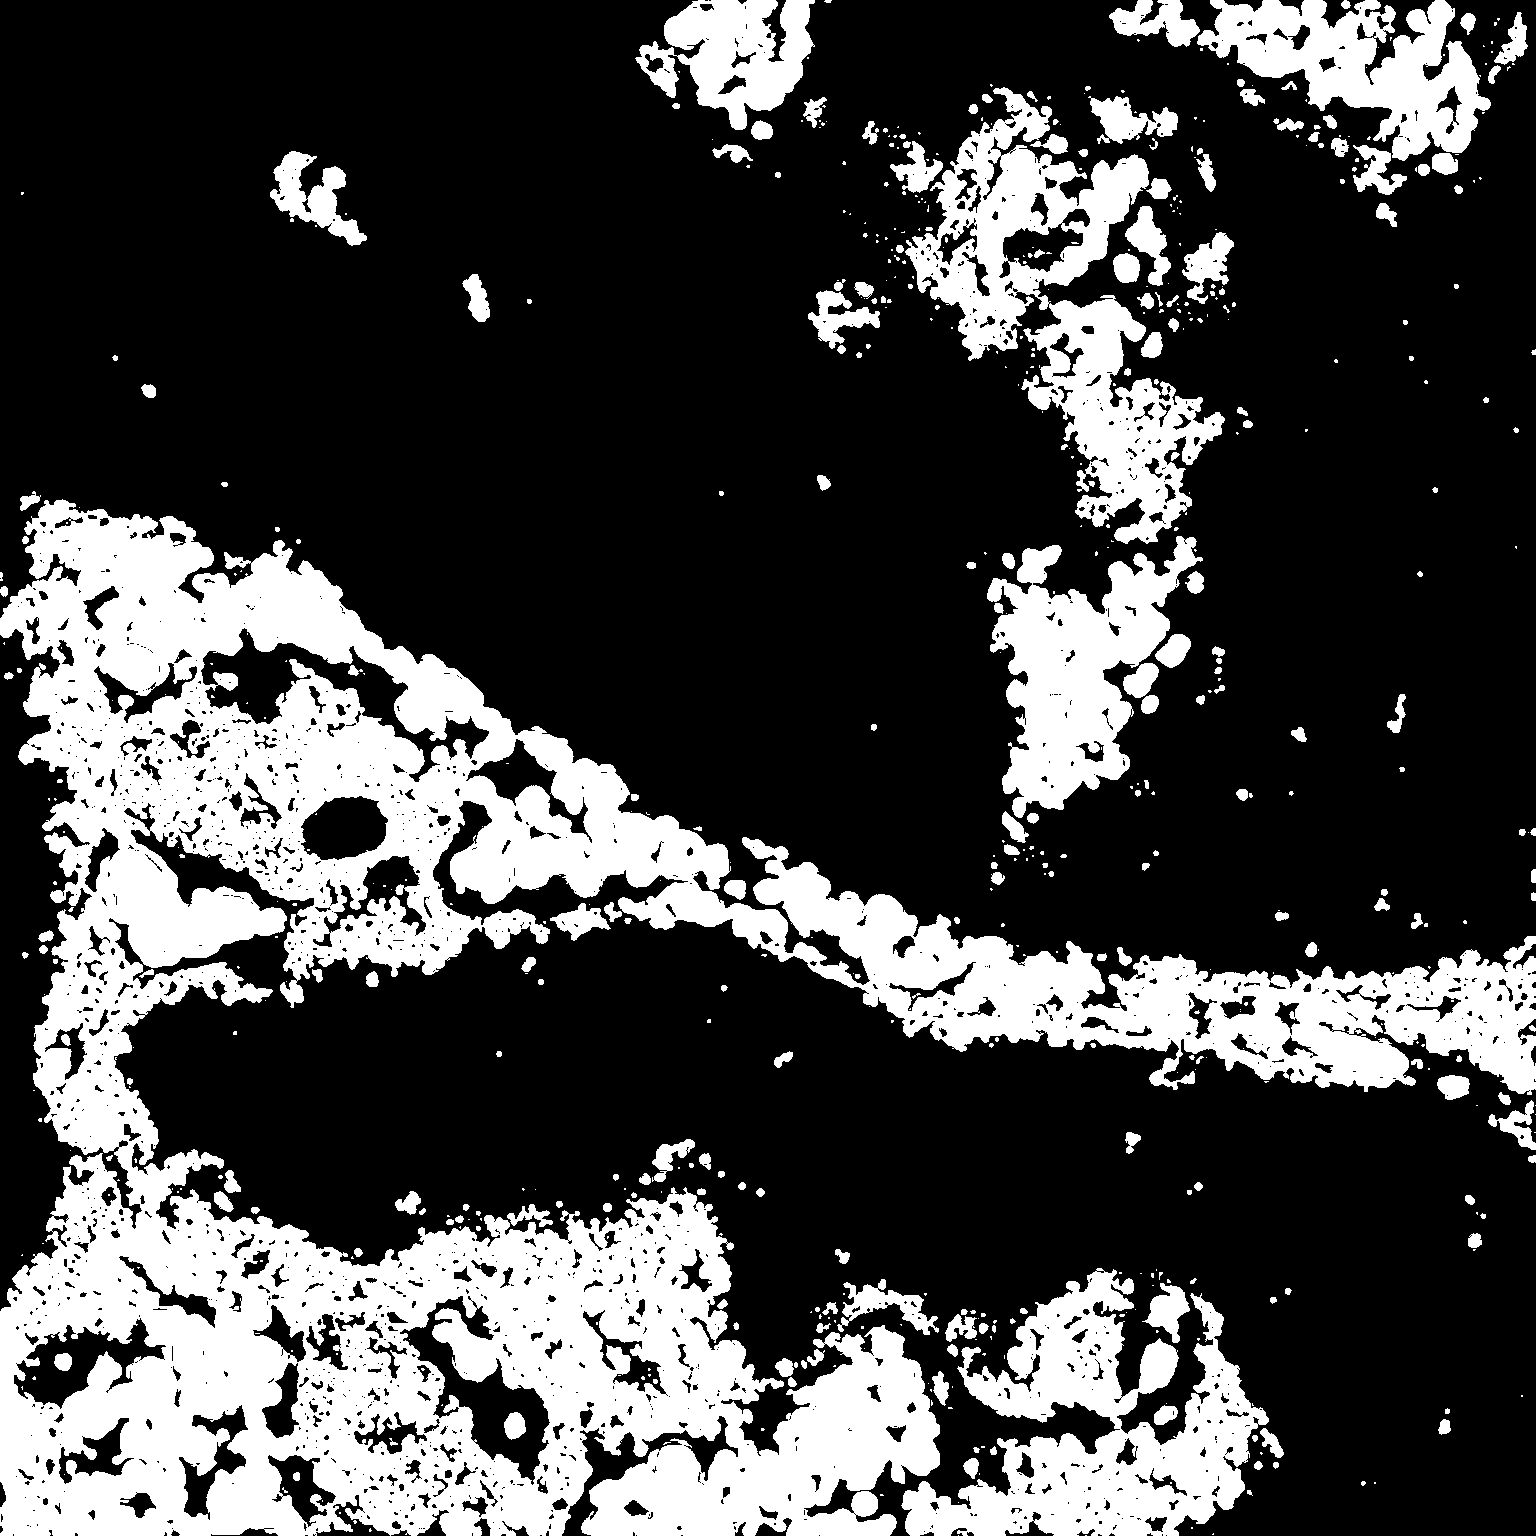
\includegraphics[width=0.24\textwidth]{figs/ch4figs/image_shortlisting/global/Percentile_HML_4C=0.png}}
	\subcaptionbox{Mean applied to \\Sample 1}{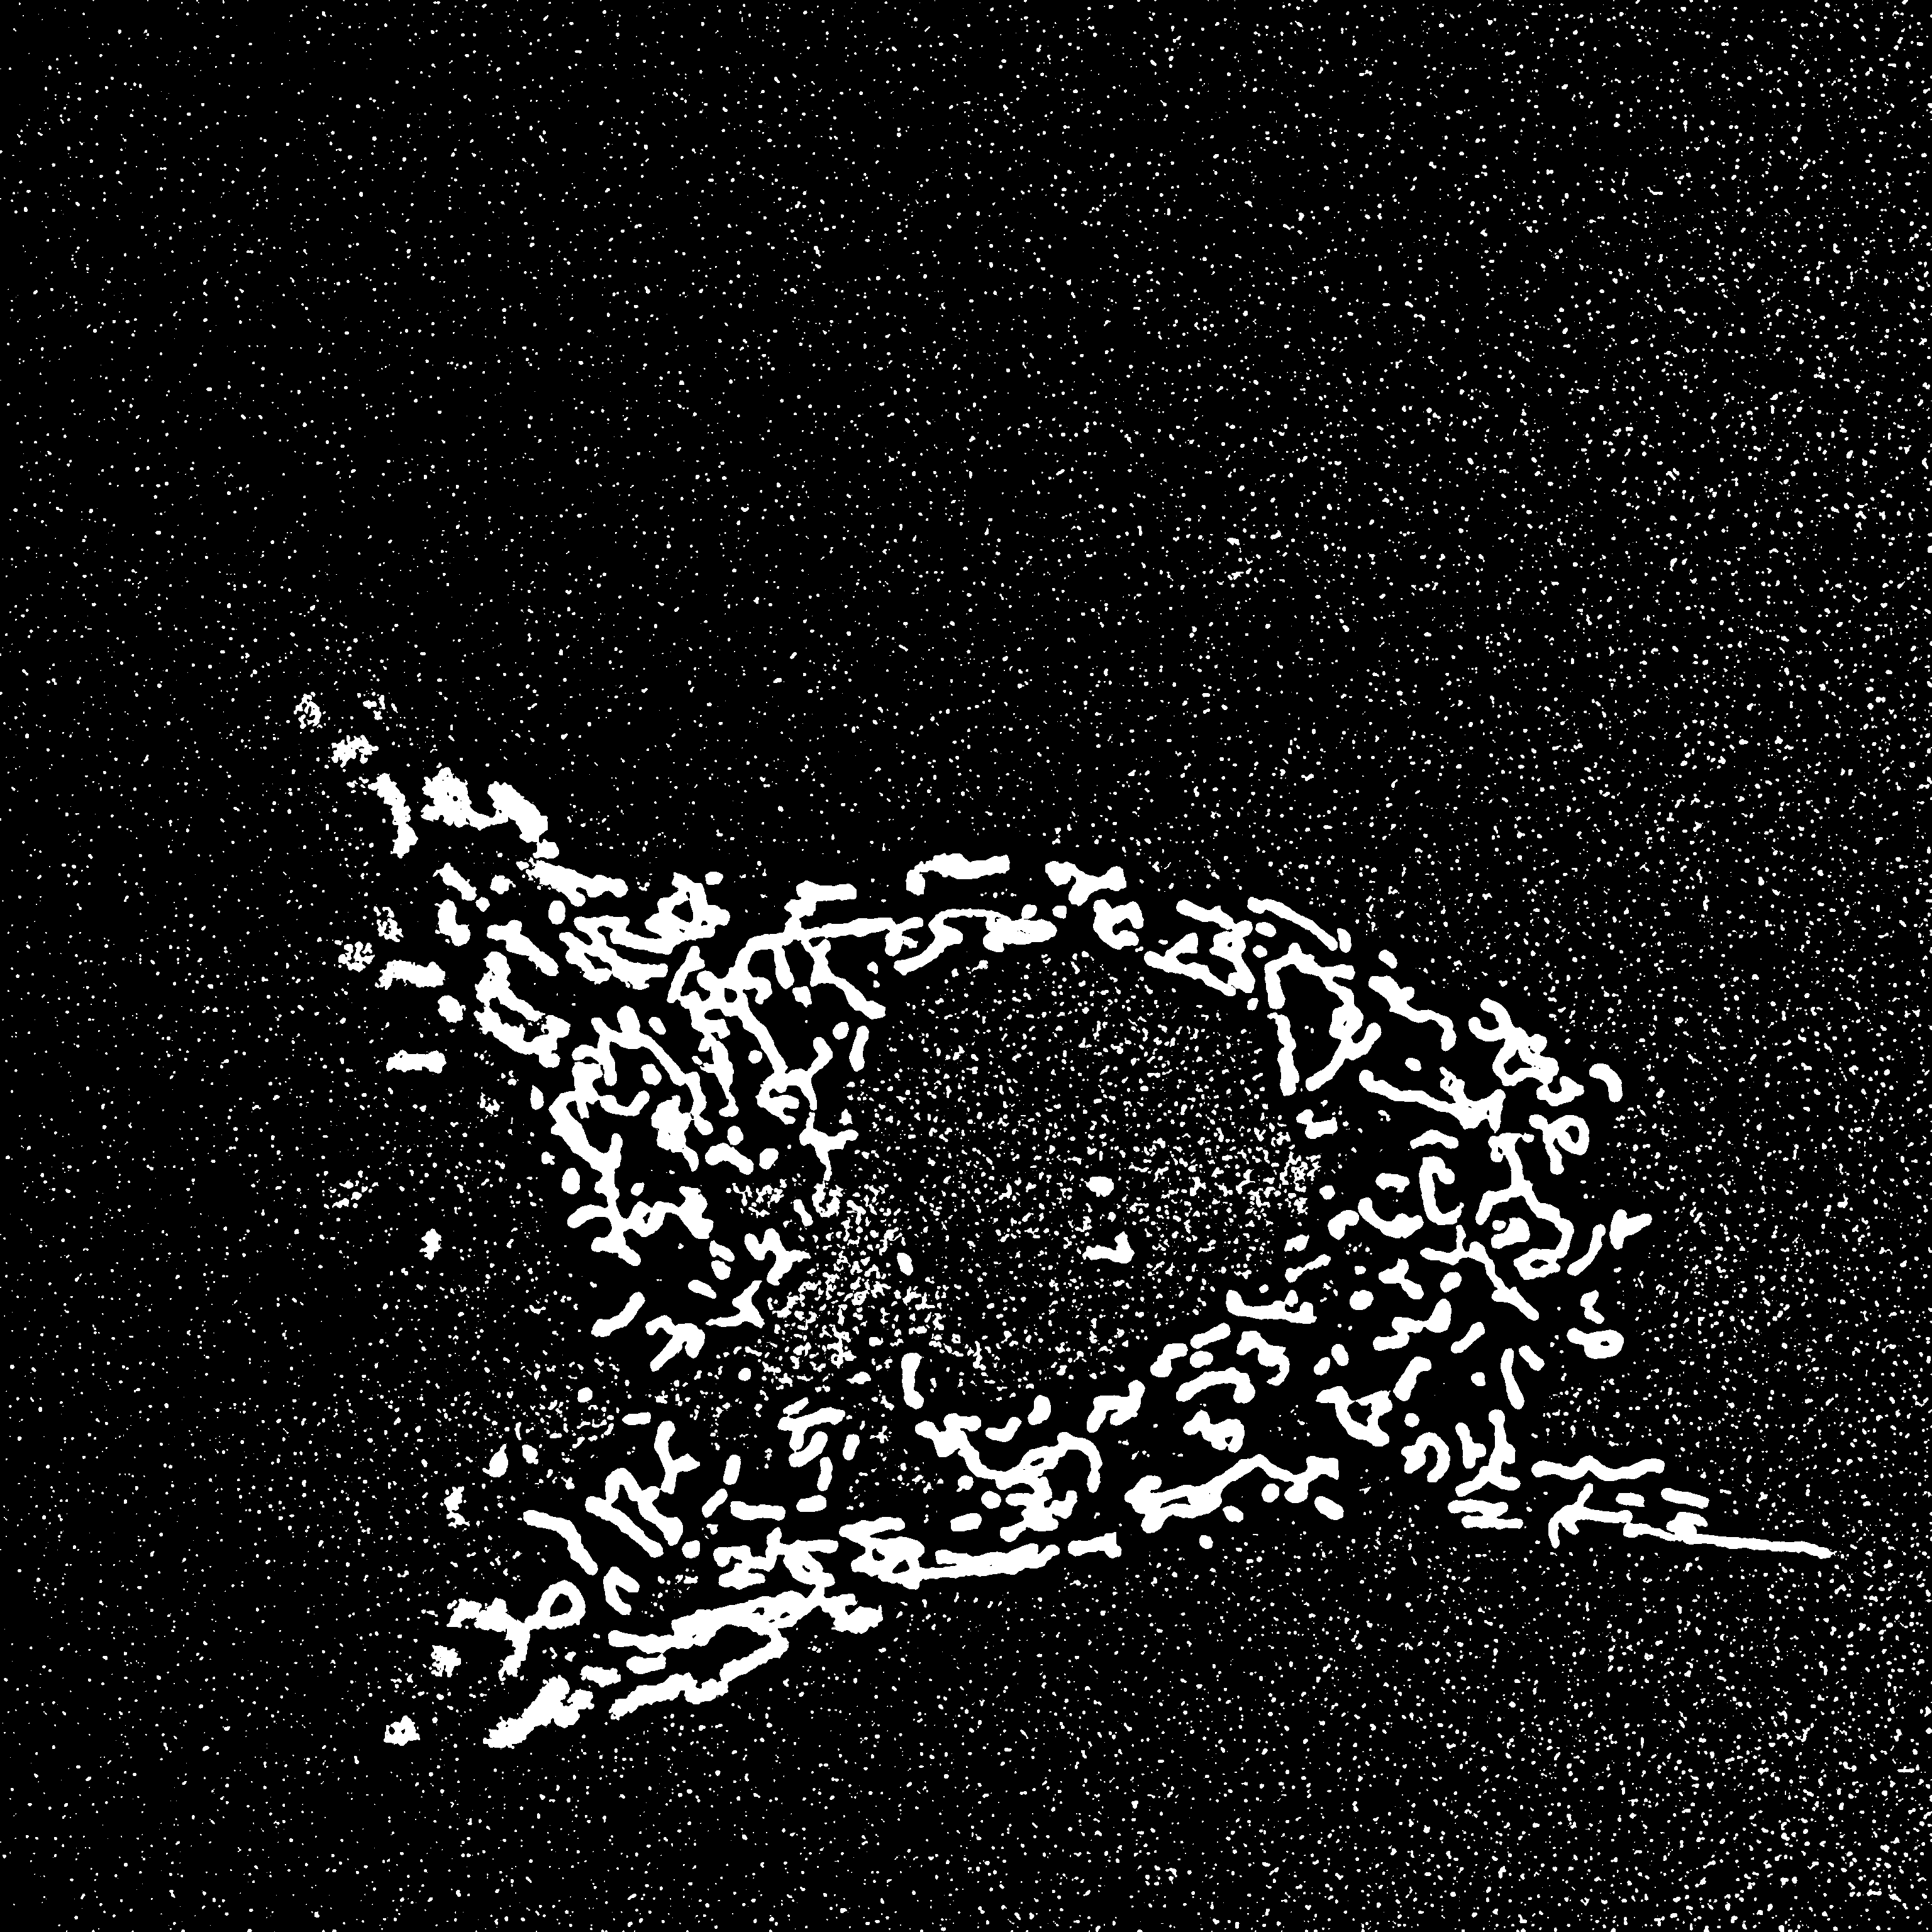
\includegraphics[width=0.24\textwidth]{figs/ch4figs/image_shortlisting/global/Mean_CCCP_1C=1T=0.png}}
	\subcaptionbox{Huang applied to Sample 4}{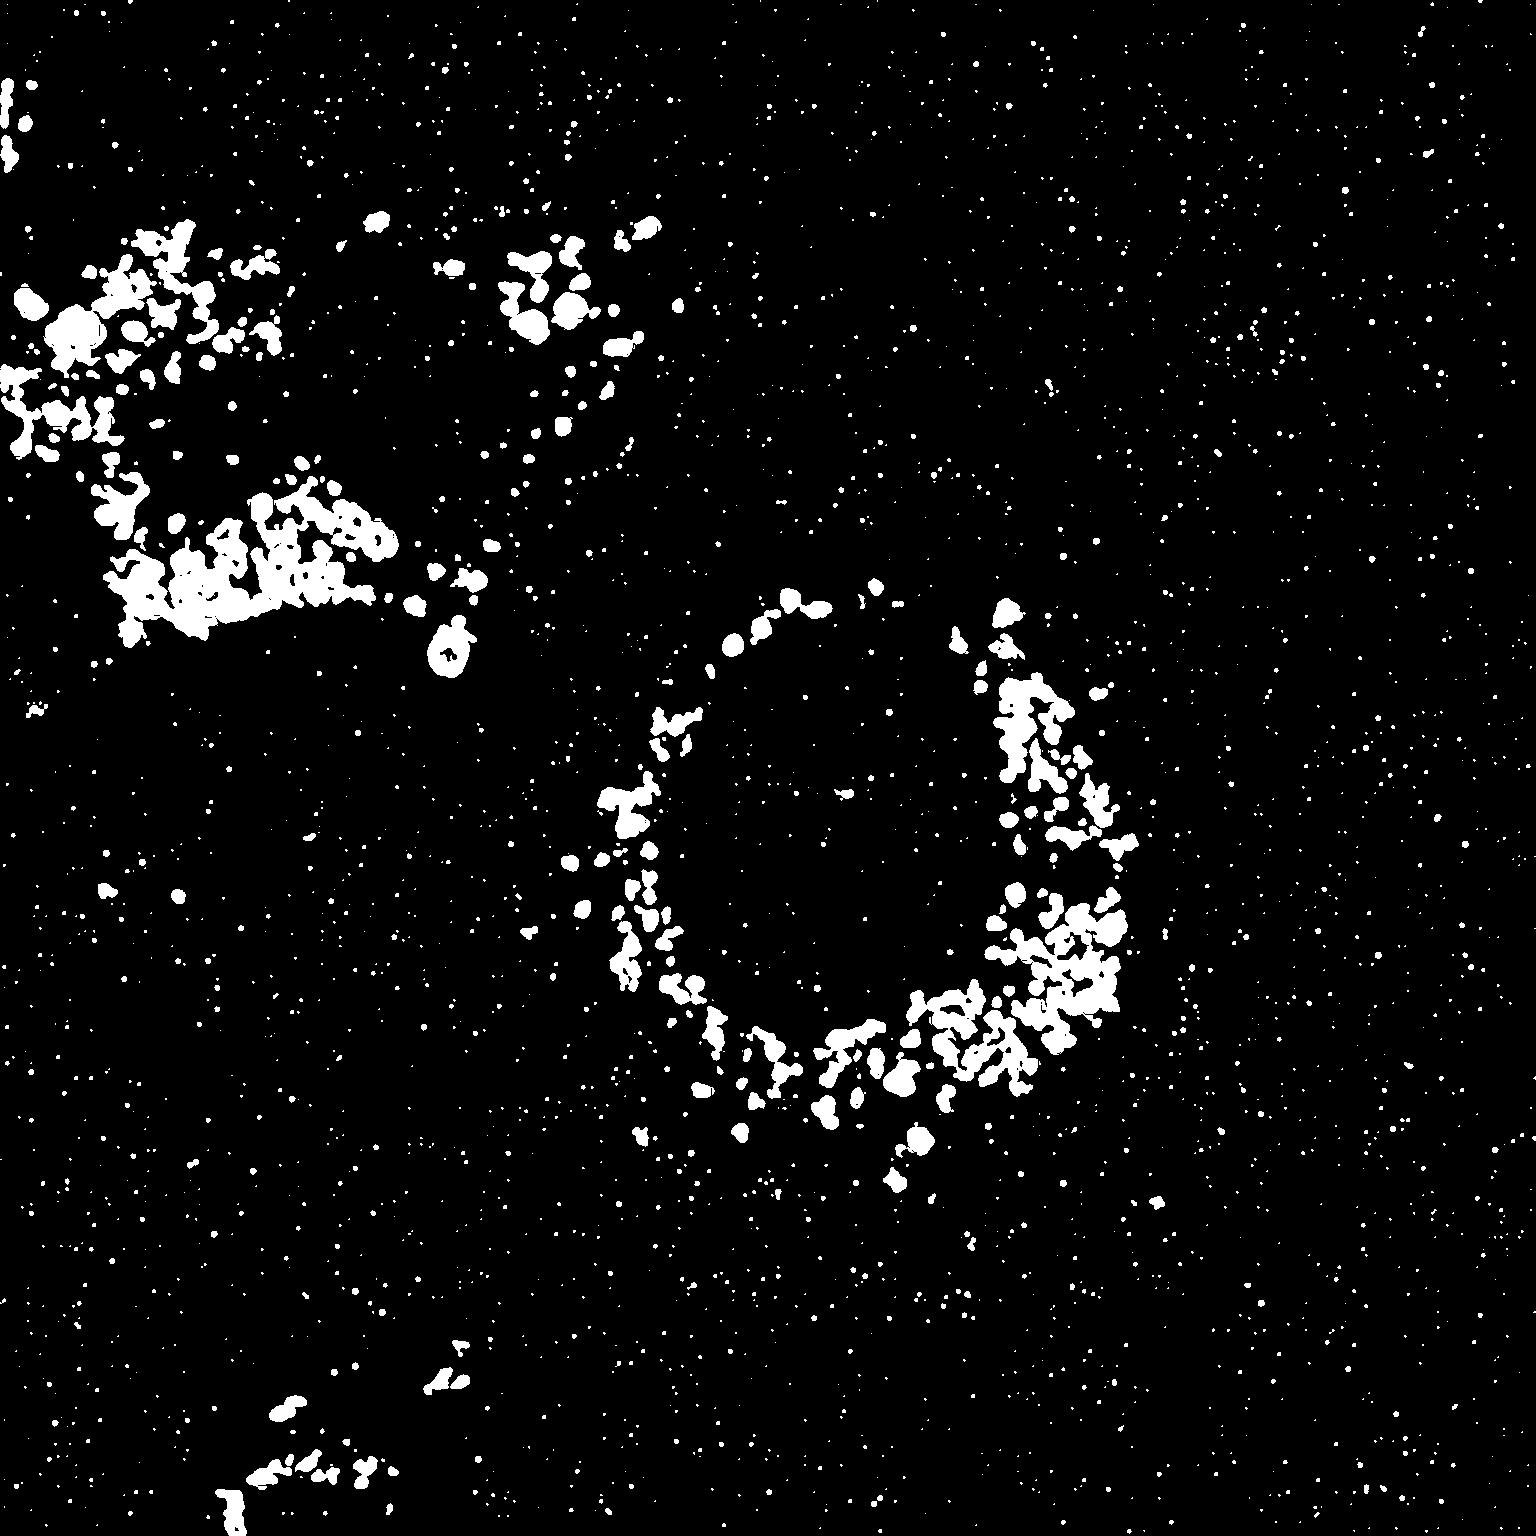
\includegraphics[width=0.24\textwidth]{figs/ch4figs/image_shortlisting/global/Huang_LML_4C=1.png}}
	\caption[Showcase of non-viable global threshold outcomes for the shortlisting data set.]{Showcase of non-viable global threshold outcomes for the shortlisting data set. The samples showcased are chosen to represent the shortcoming of these methods for the real sample images shown in Figure \ref{fig:shortlist_raw}.}
	\label{fig:bad_global_subset}
\end{figure}
\FloatBarrier
\subsection{Local threshold shortlisting}
A total of 9 local thresholding methods, provided by the \textit{Auto Local Threshold} plug-in, were evaluated for viable application to the sample images. These methods are:
\begin{multicols}{3}
	\begin{itemize}
		\setlength\itemsep{1mm}
		\item Bernsen
		\item Contrast
		\item Mean
		\item Median
		\item MidGrey
		\item Niblack
		\item Otsu
		\item Phansalkar
		\item Sauvola
	\end{itemize}
\end{multicols}
Compared to global thresholding methods, the shortlisting of local thresholding methods is a bit more involved due to the tuning of parameters being required for fair evaluation of these methods. All local thresholding methods binarise each pixel based on a pixel-specific threshold where this threshold is determined using a localized region, or window, surrounding said pixel. The size of this neighbourhood can greatly influence the binarisation outcome thus selection of an appropriate window size for each image is crucial for every method. Additionally, all local thresholding methods being assessed, save for Contrast and Otsu, provide additional parameters that can be tuned to further influence the binarisation. For rapid application of these local thresholds it is not uncommon to approximate parameters that best generalize across the sample set based on the binarisation performance for a smaller subset. For this reason, the shortlisting will evaluate the local thresholding methods with performance considered with respect to the parameter selections, per method, that generalize best across all of the shortlisting samples. 
\paragraph{Findings:} From observing the binarisation results of the local thresholding methods it was determined that Bernsen, Mean, Median, and MidGrey will be used for further evaluations as they provide the best balance between consistency and performance compared to the other local thresholding methods. From Figure \ref{fig:local_window_size_showcase}, it is observed that for the MidGrey method that increasing the window size parameter increases the exclusion of foreground voxels, shown in Figure \ref{fig:local_window_size_showcase}(\subref{subfig:mg_w15}-\subref{subfig:mg_w100}), while the opposite occurs for the Median threshold, shown in Figure \ref{fig:local_window_size_showcase}(\subref{subfig:mg_w15}-\subref{subfig:mg_w100}). The behaviour seen in MidGrey is also experienced with Bernsen thresholding while the Mean threshold is similar to that of the Median threshold. While this does not imply either the exclusion of actual foreground structures or inclusion of definite background structures into foreground respectively, but it does imply an increasing risk of either occurring. For this reason a window size of $15$ was selected as it generalized well across the shortlist sample images for all of the local thresholding methods that have been accepted for use in further evaluations. For the secondary parameters, the \textit{contrast threshold} of the Bernsen thresholding was selected as $20$ due to it decreasing the quantity of background inclusion in the image with no noticeable impact on the foreground structures themselves present in Figures \ref{fig:local_param_tuning}~(\subref{subfig:bern_10}-\subref{subfig:bern_20}) although it is noted that Bernsen does not perform very well for this sample, being nigh unusable for certain analysis, due to the heavy fragmentation of the foreground structures. The Mean, Median, and MidGrey method all have an identical \textit{subtraction constant} parameter which performs best for values less than $0$ with values greater than this inducing extreme background inclusion, seen in Figures \ref{fig:local_param_tuning}(\subref{subfig:midG_-5}-\subref{subfig:midG_5}), due to this fixed positive constant reducing the threshold to zero, or below, when the threshold calculated for said window is less than of the constant. This is what induces the large white regions seen in Figure \ref{fig:local_param_tuning}(\subref{subfig:midG_5}) with only the regions along the structure edges, that fall within the window, producing a threshold value exceeding the \textit{subtraction constant}. Using a negative value for this constant results in the increased strictness of the threshold applied to every voxel by these methods. From this it was observed that a value of $-5$ resulted in sufficiently good outcomes with no noticeably detrimental foreground exclusion or background inclusion with this value for all three of the related local thresholding methods. A showcase of the binarisation outcomes for all of the tested local thresholding methods across a range of window parameter sizes is shown in Section \ref{appen_sec:local_shortlist}.

\begin{figure}
	\centering
	\subcaptionbox{Median with a\\Window size of 15\label{subfig:md_w15}}{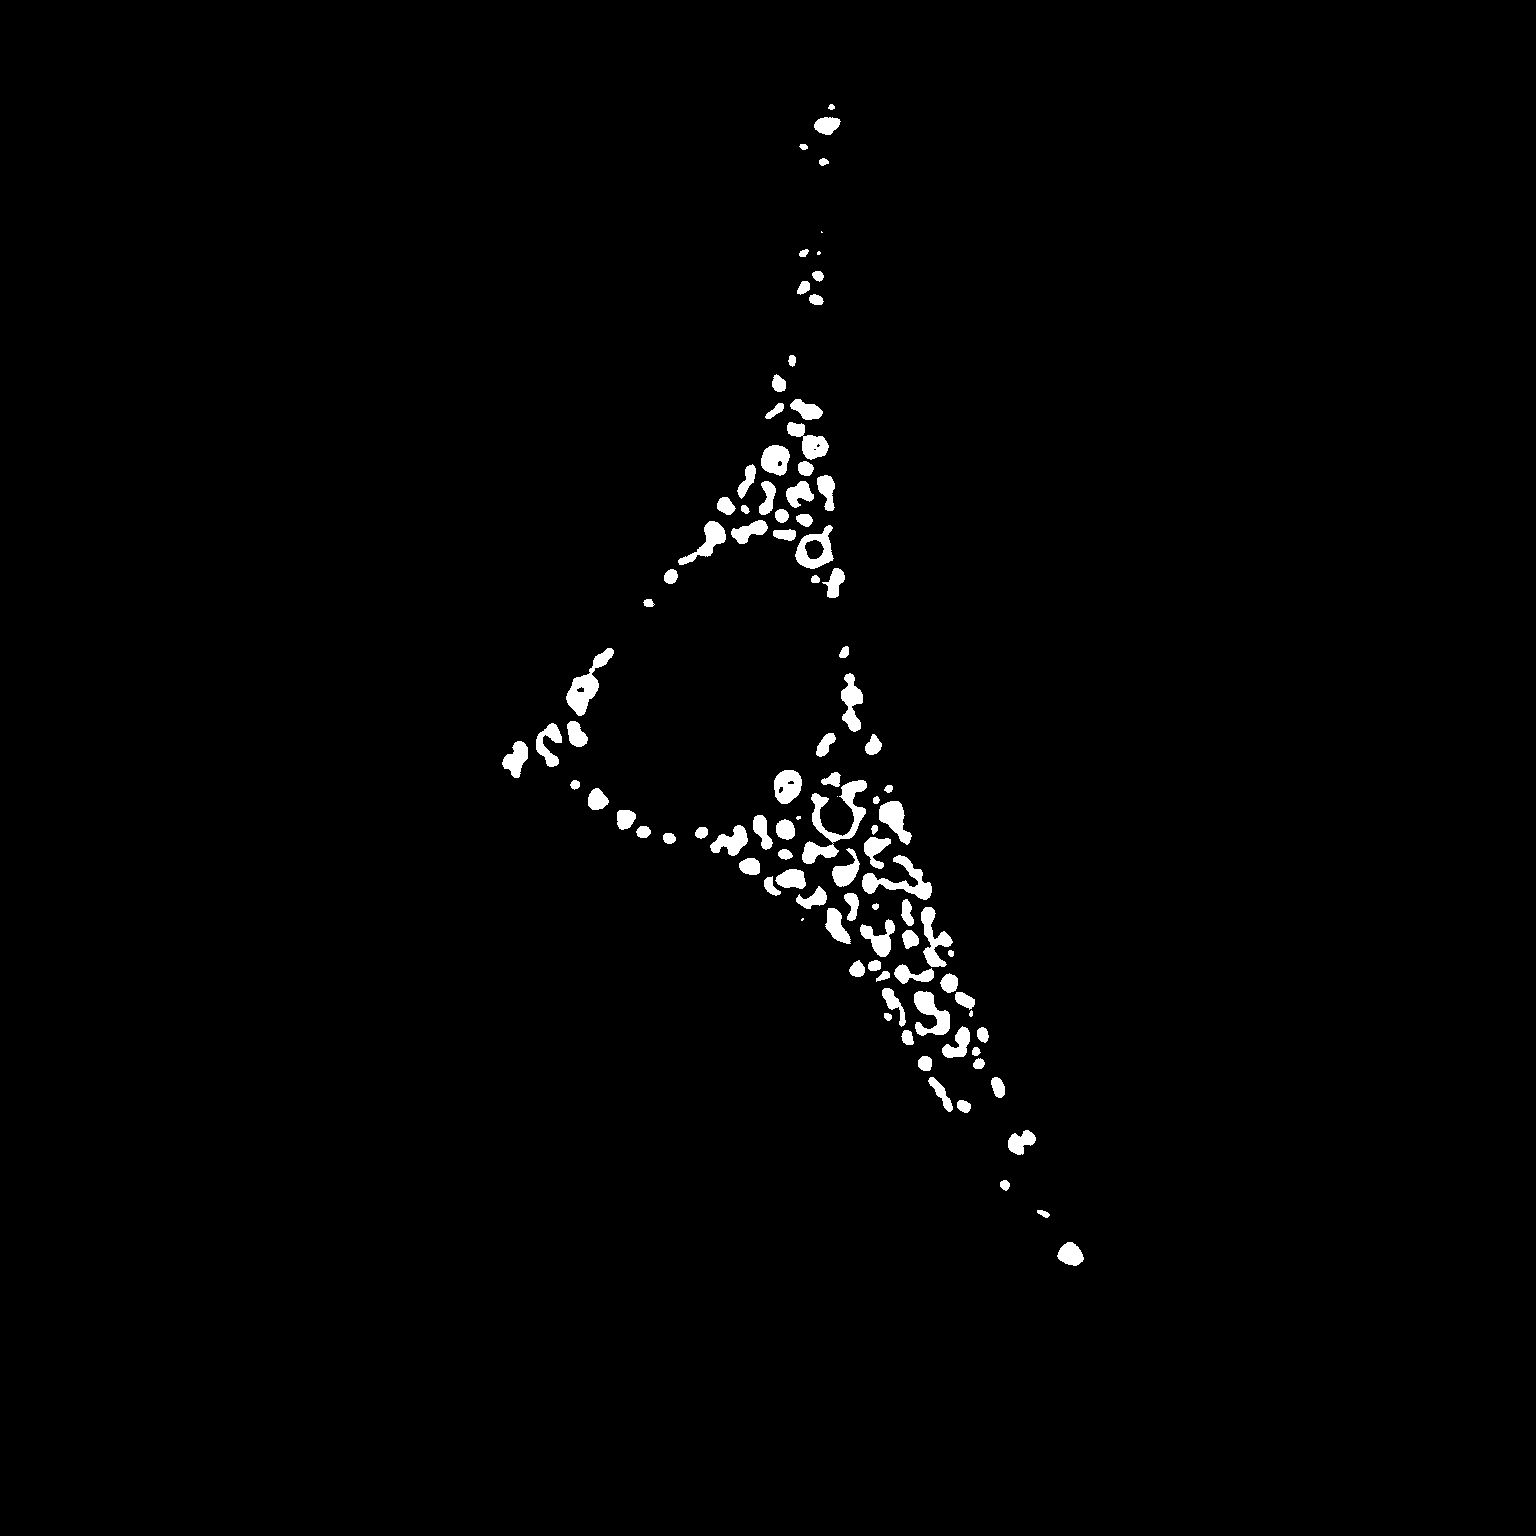
\includegraphics[width=0.3\textwidth]{figs/ch4figs/image_shortlisting/local/Median_p-5_w15_LML_3C=0.png}}
	\subcaptionbox{Median with a\\Window size of 60\label{subfig:md_w60}}{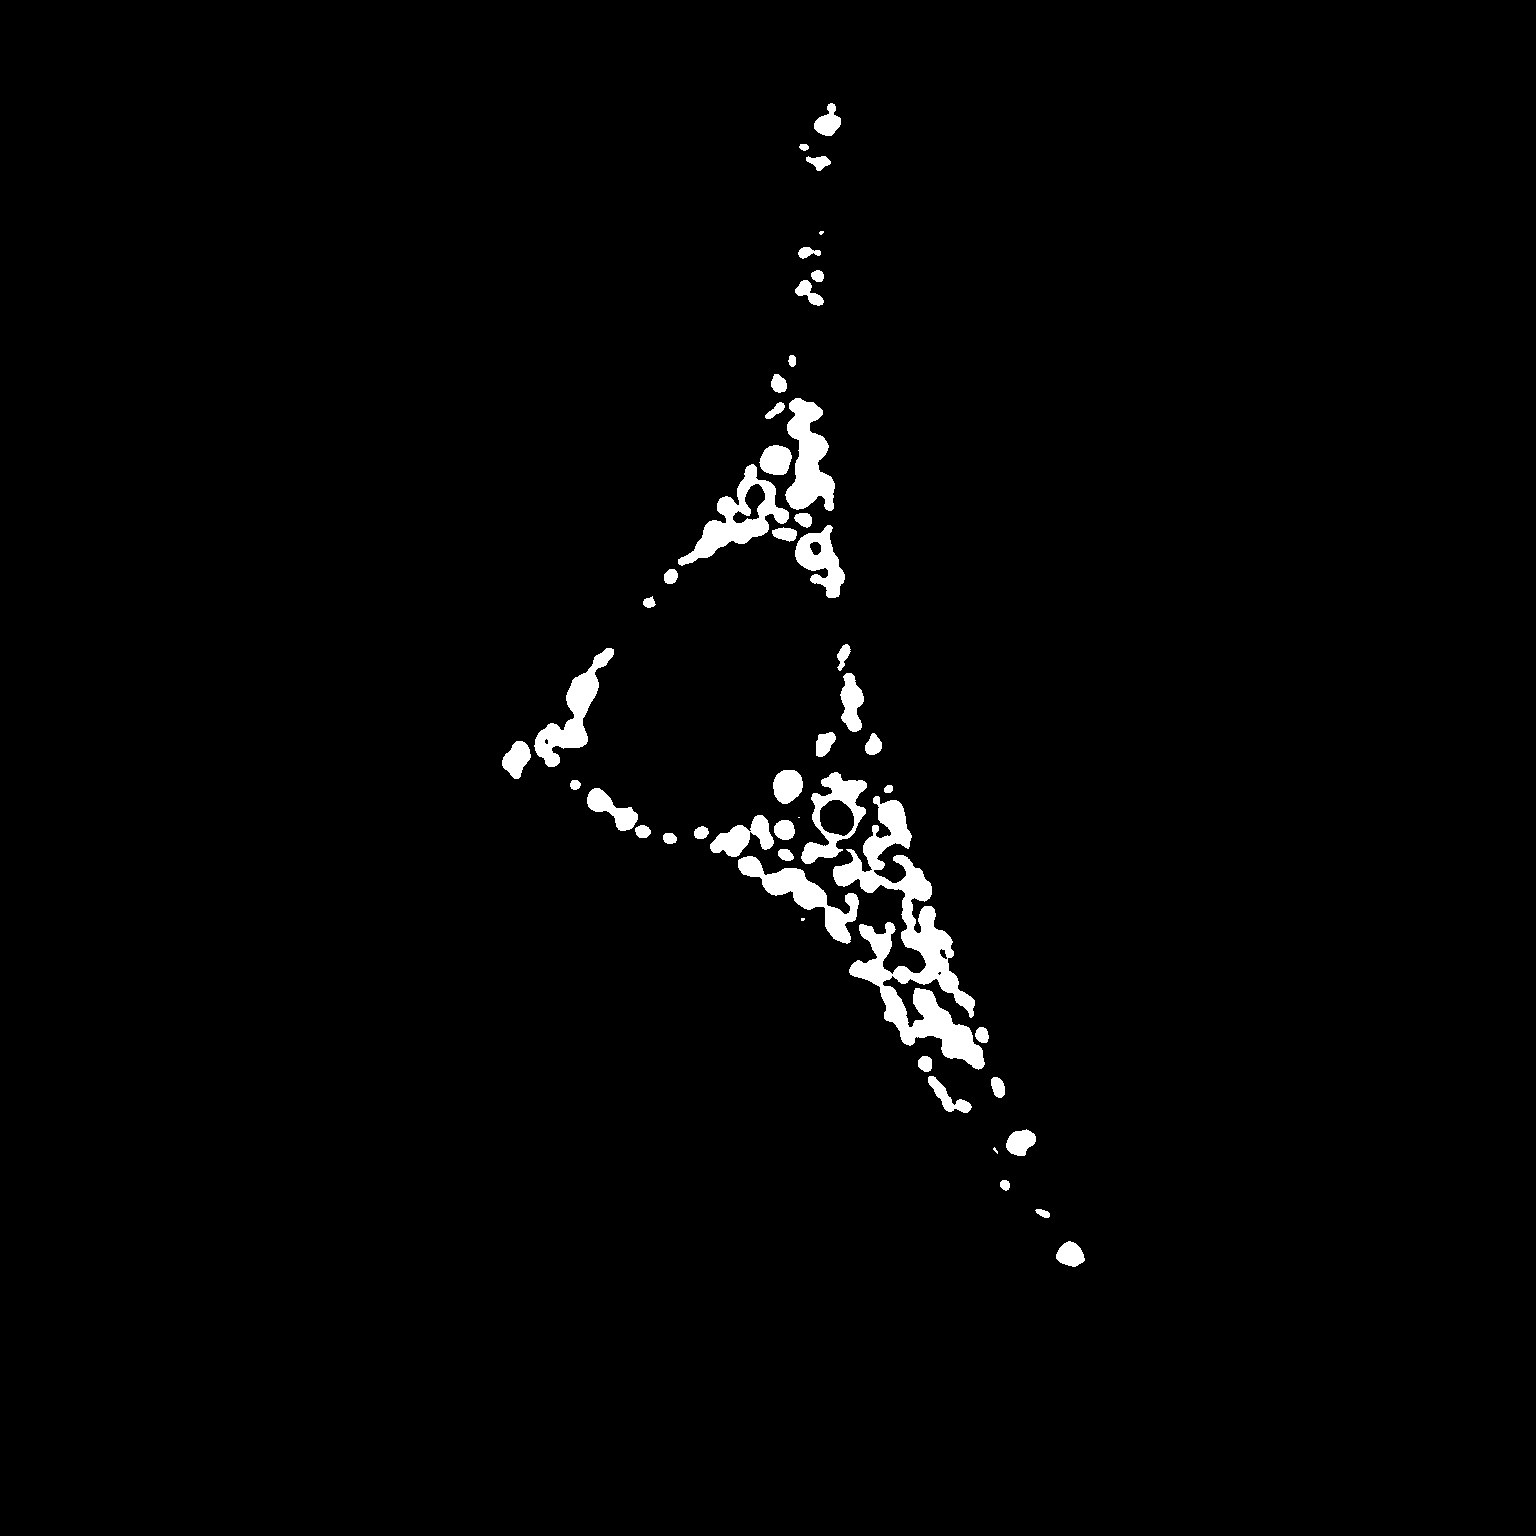
\includegraphics[width=0.3\textwidth]{figs/ch4figs/image_shortlisting/local/Median_p-5_w60_LML_3C=0.png}}
	\subcaptionbox{Median with a\\Window size of 100\label{subfig:md_w100}}{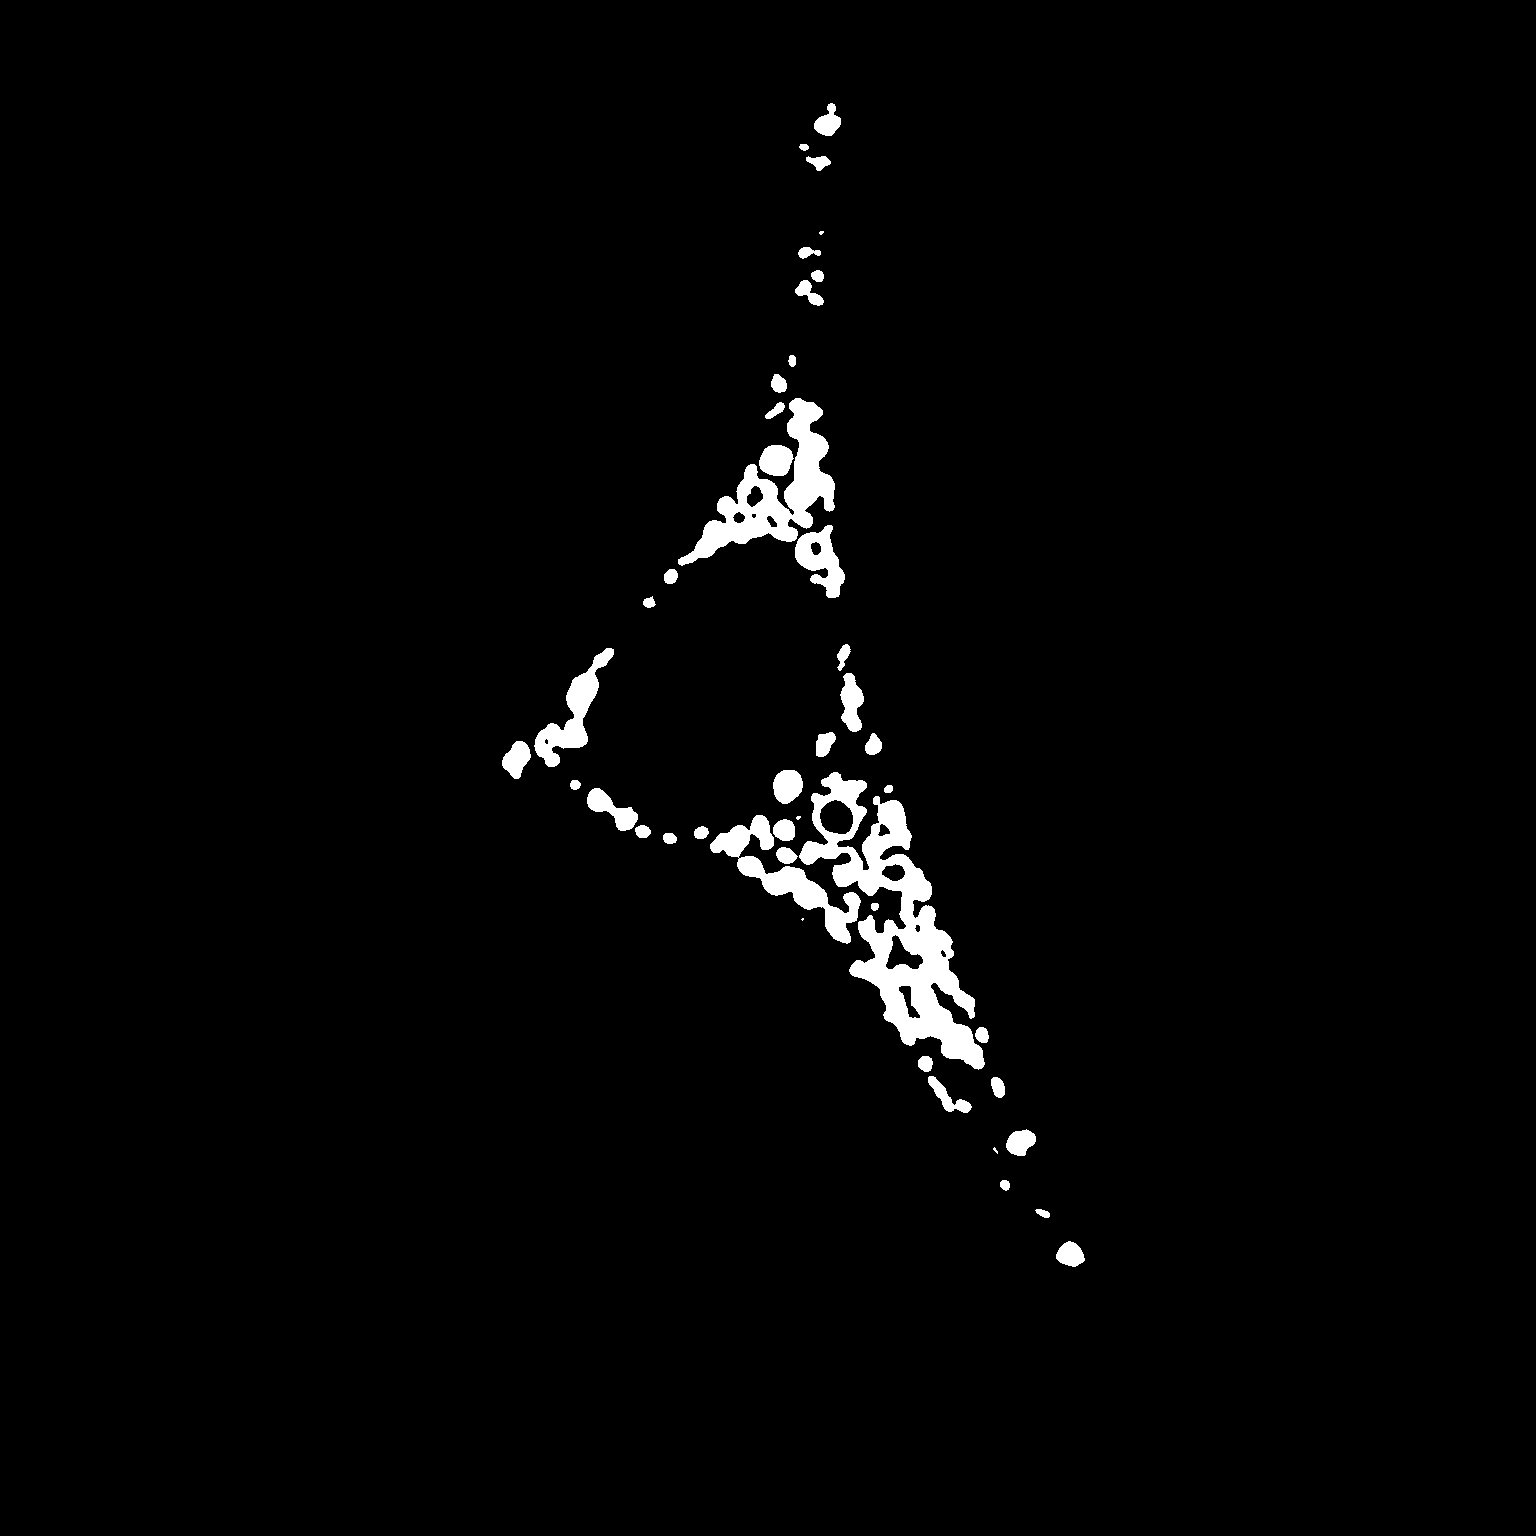
\includegraphics[width=0.3\textwidth]{figs/ch4figs/image_shortlisting/local/Median_p-5_w100_LML_3C=0.png}}
	\subcaptionbox{MidGrey with a\\Window size of 15\label{subfig:mg_w15}}{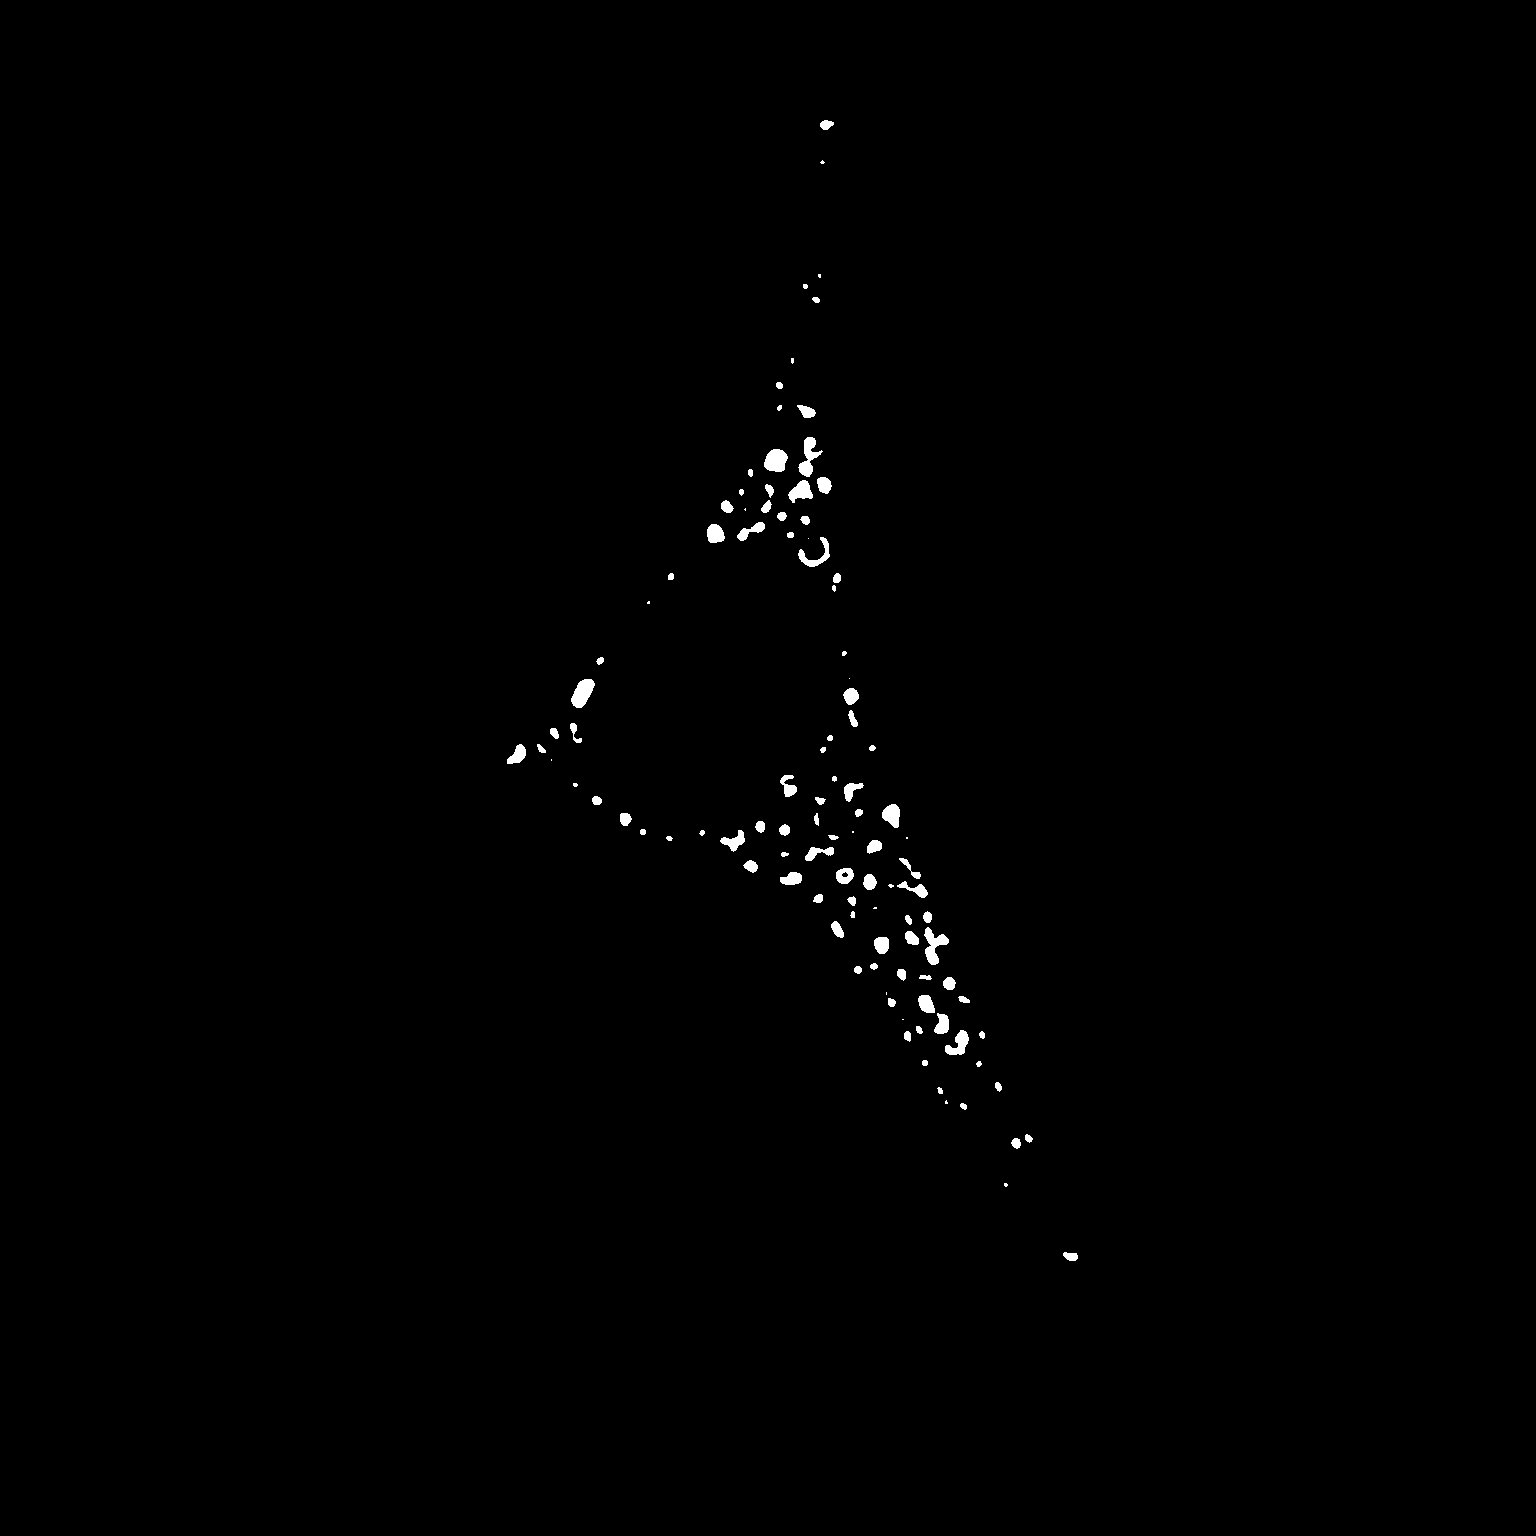
\includegraphics[width=0.3\textwidth]{figs/ch4figs/image_shortlisting/local/MidGrey_p-5_w15_LML_3C=0.png}}
	\subcaptionbox{MidGrey with a\\Window size of 60\label{subfig:mg_w60}}{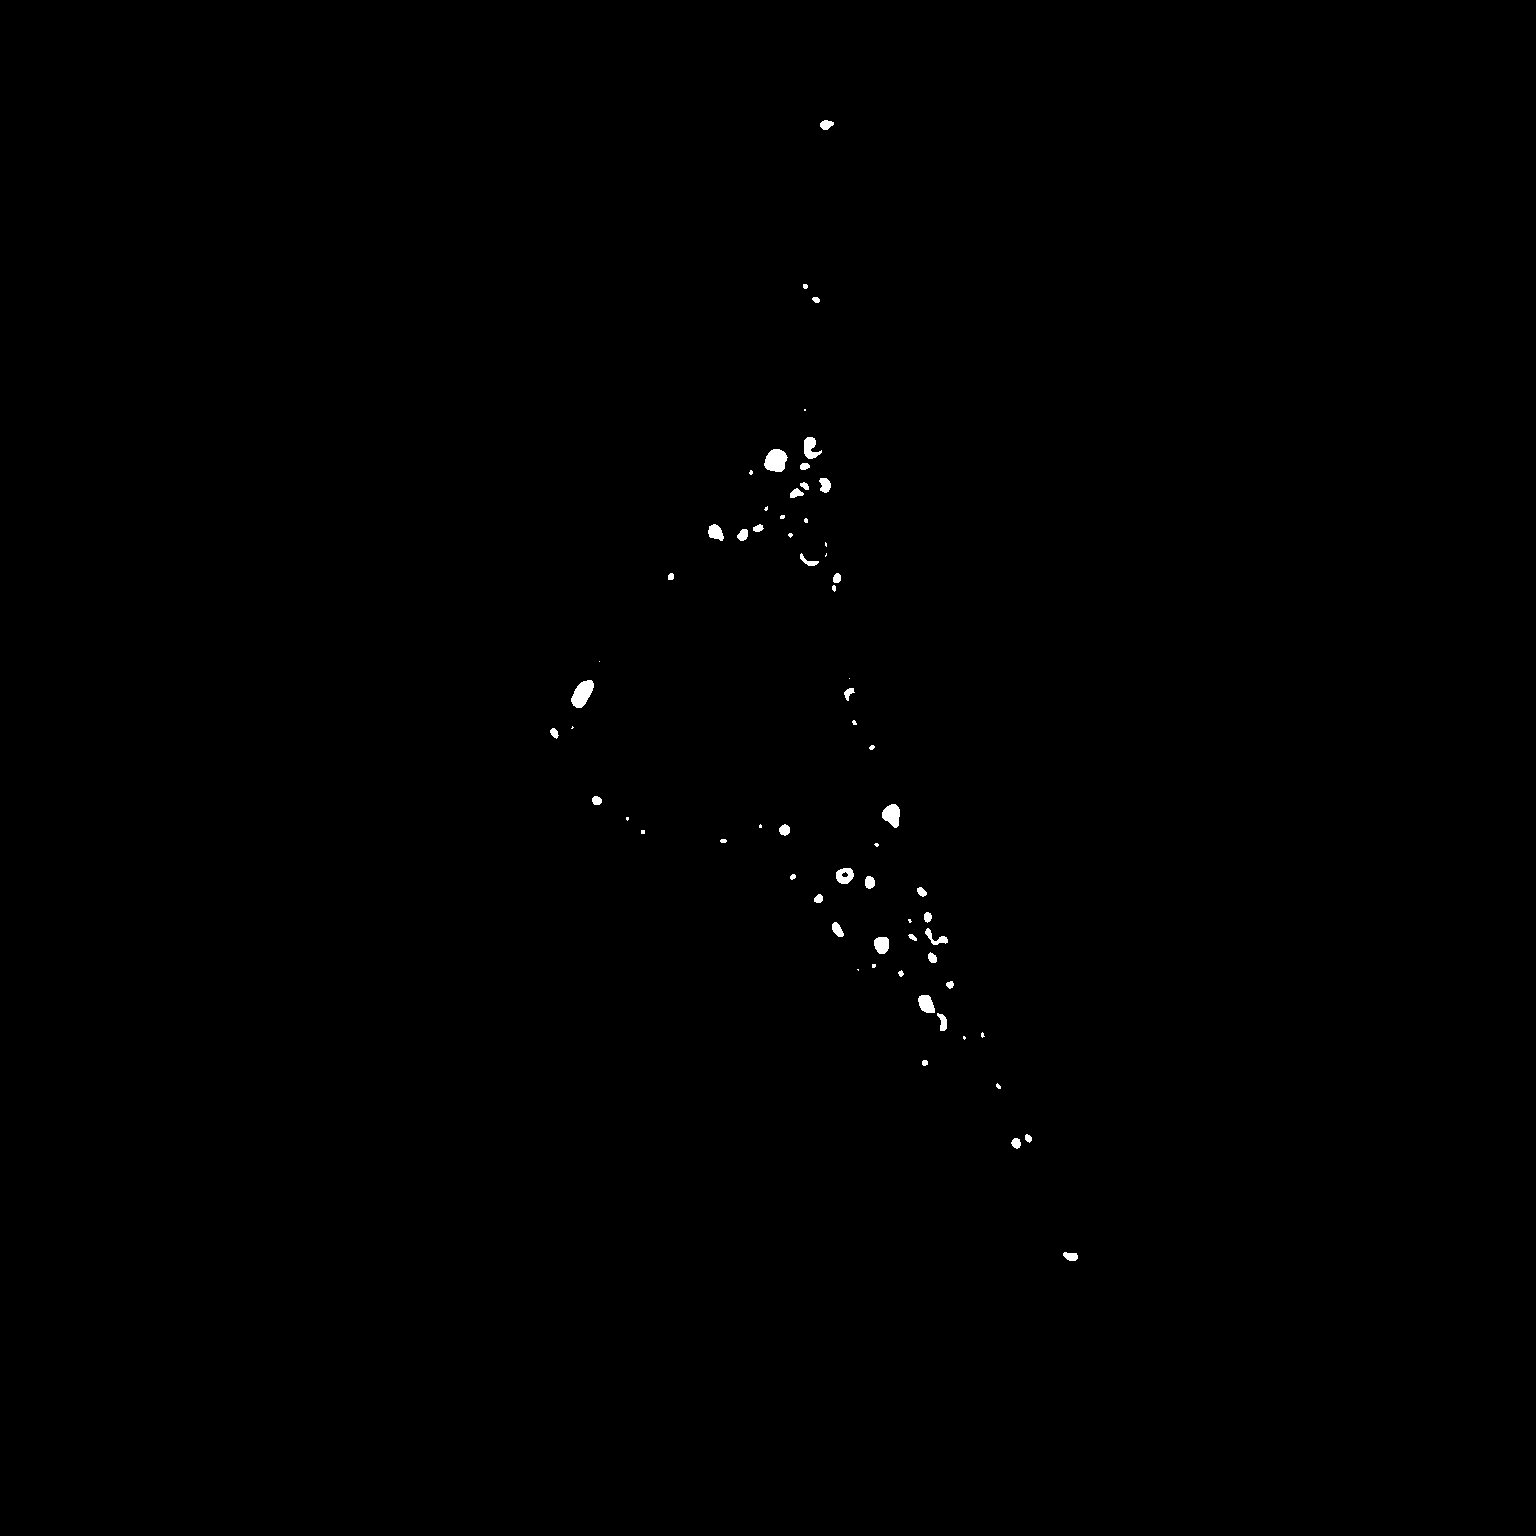
\includegraphics[width=0.3\textwidth]{figs/ch4figs/image_shortlisting/local/MidGrey_p-5_w60_LML_3C=0.png}}
	\subcaptionbox{MidGrey with a\\Window size of 100\label{subfig:mg_w100}}{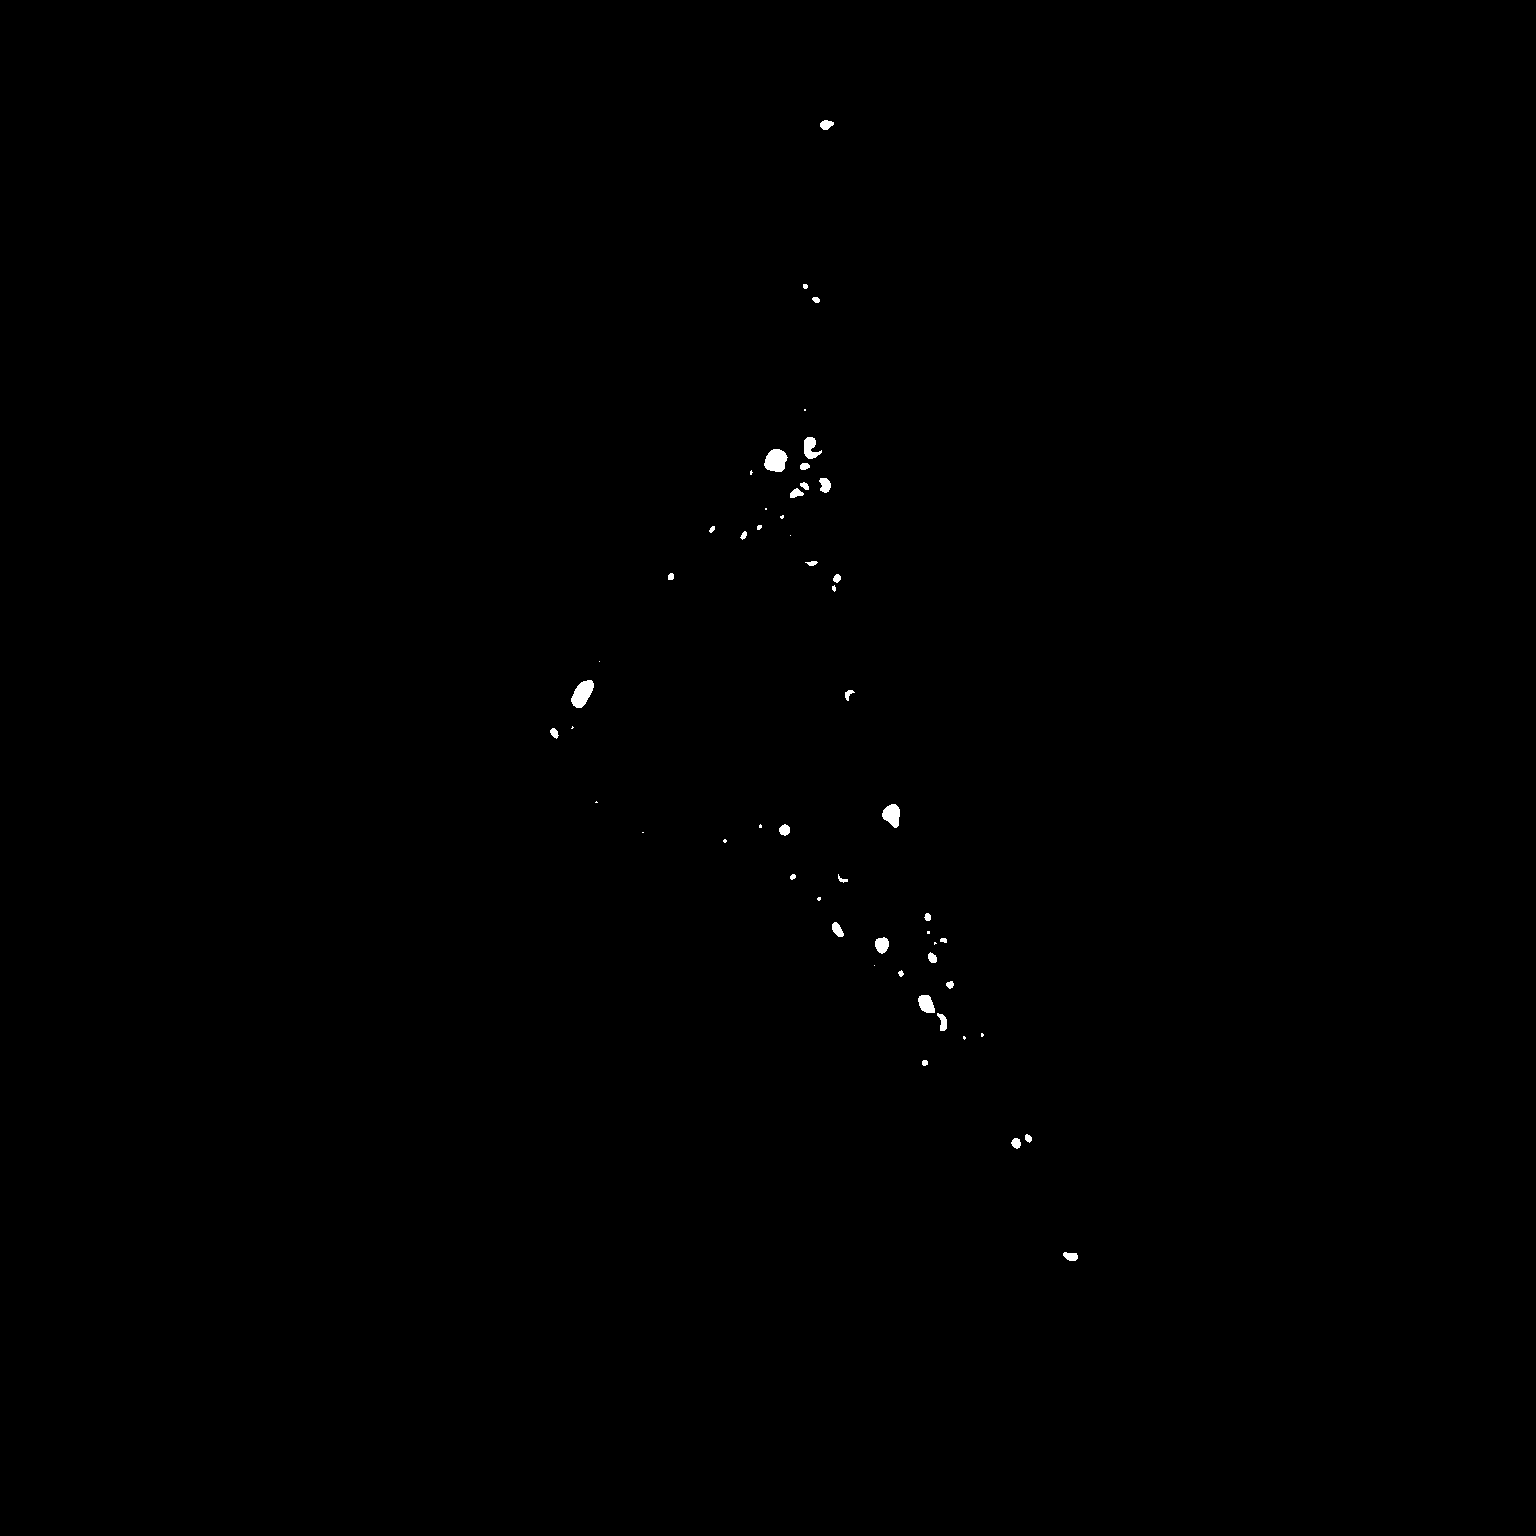
\includegraphics[width=0.3\textwidth]{figs/ch4figs/image_shortlisting/local/MidGrey_p-5_w100_LML_3C=0.png}}
	\caption[Showcasing the impact larger window sizes can have on local thresholding outcomes.]{Showcasing the impact larger window sizes can have on local thresholding outcomes. For this example the Median and MidGrey thresholding methods have been applied to sample $3$ with a subtraction constant of $-5$.}
	\label{fig:local_window_size_showcase}
\end{figure}
 
\begin{figure}
	\centering
	\subcaptionbox{Bernsen thresholding with a contrast threshold of 10\label{subfig:bern_10}}{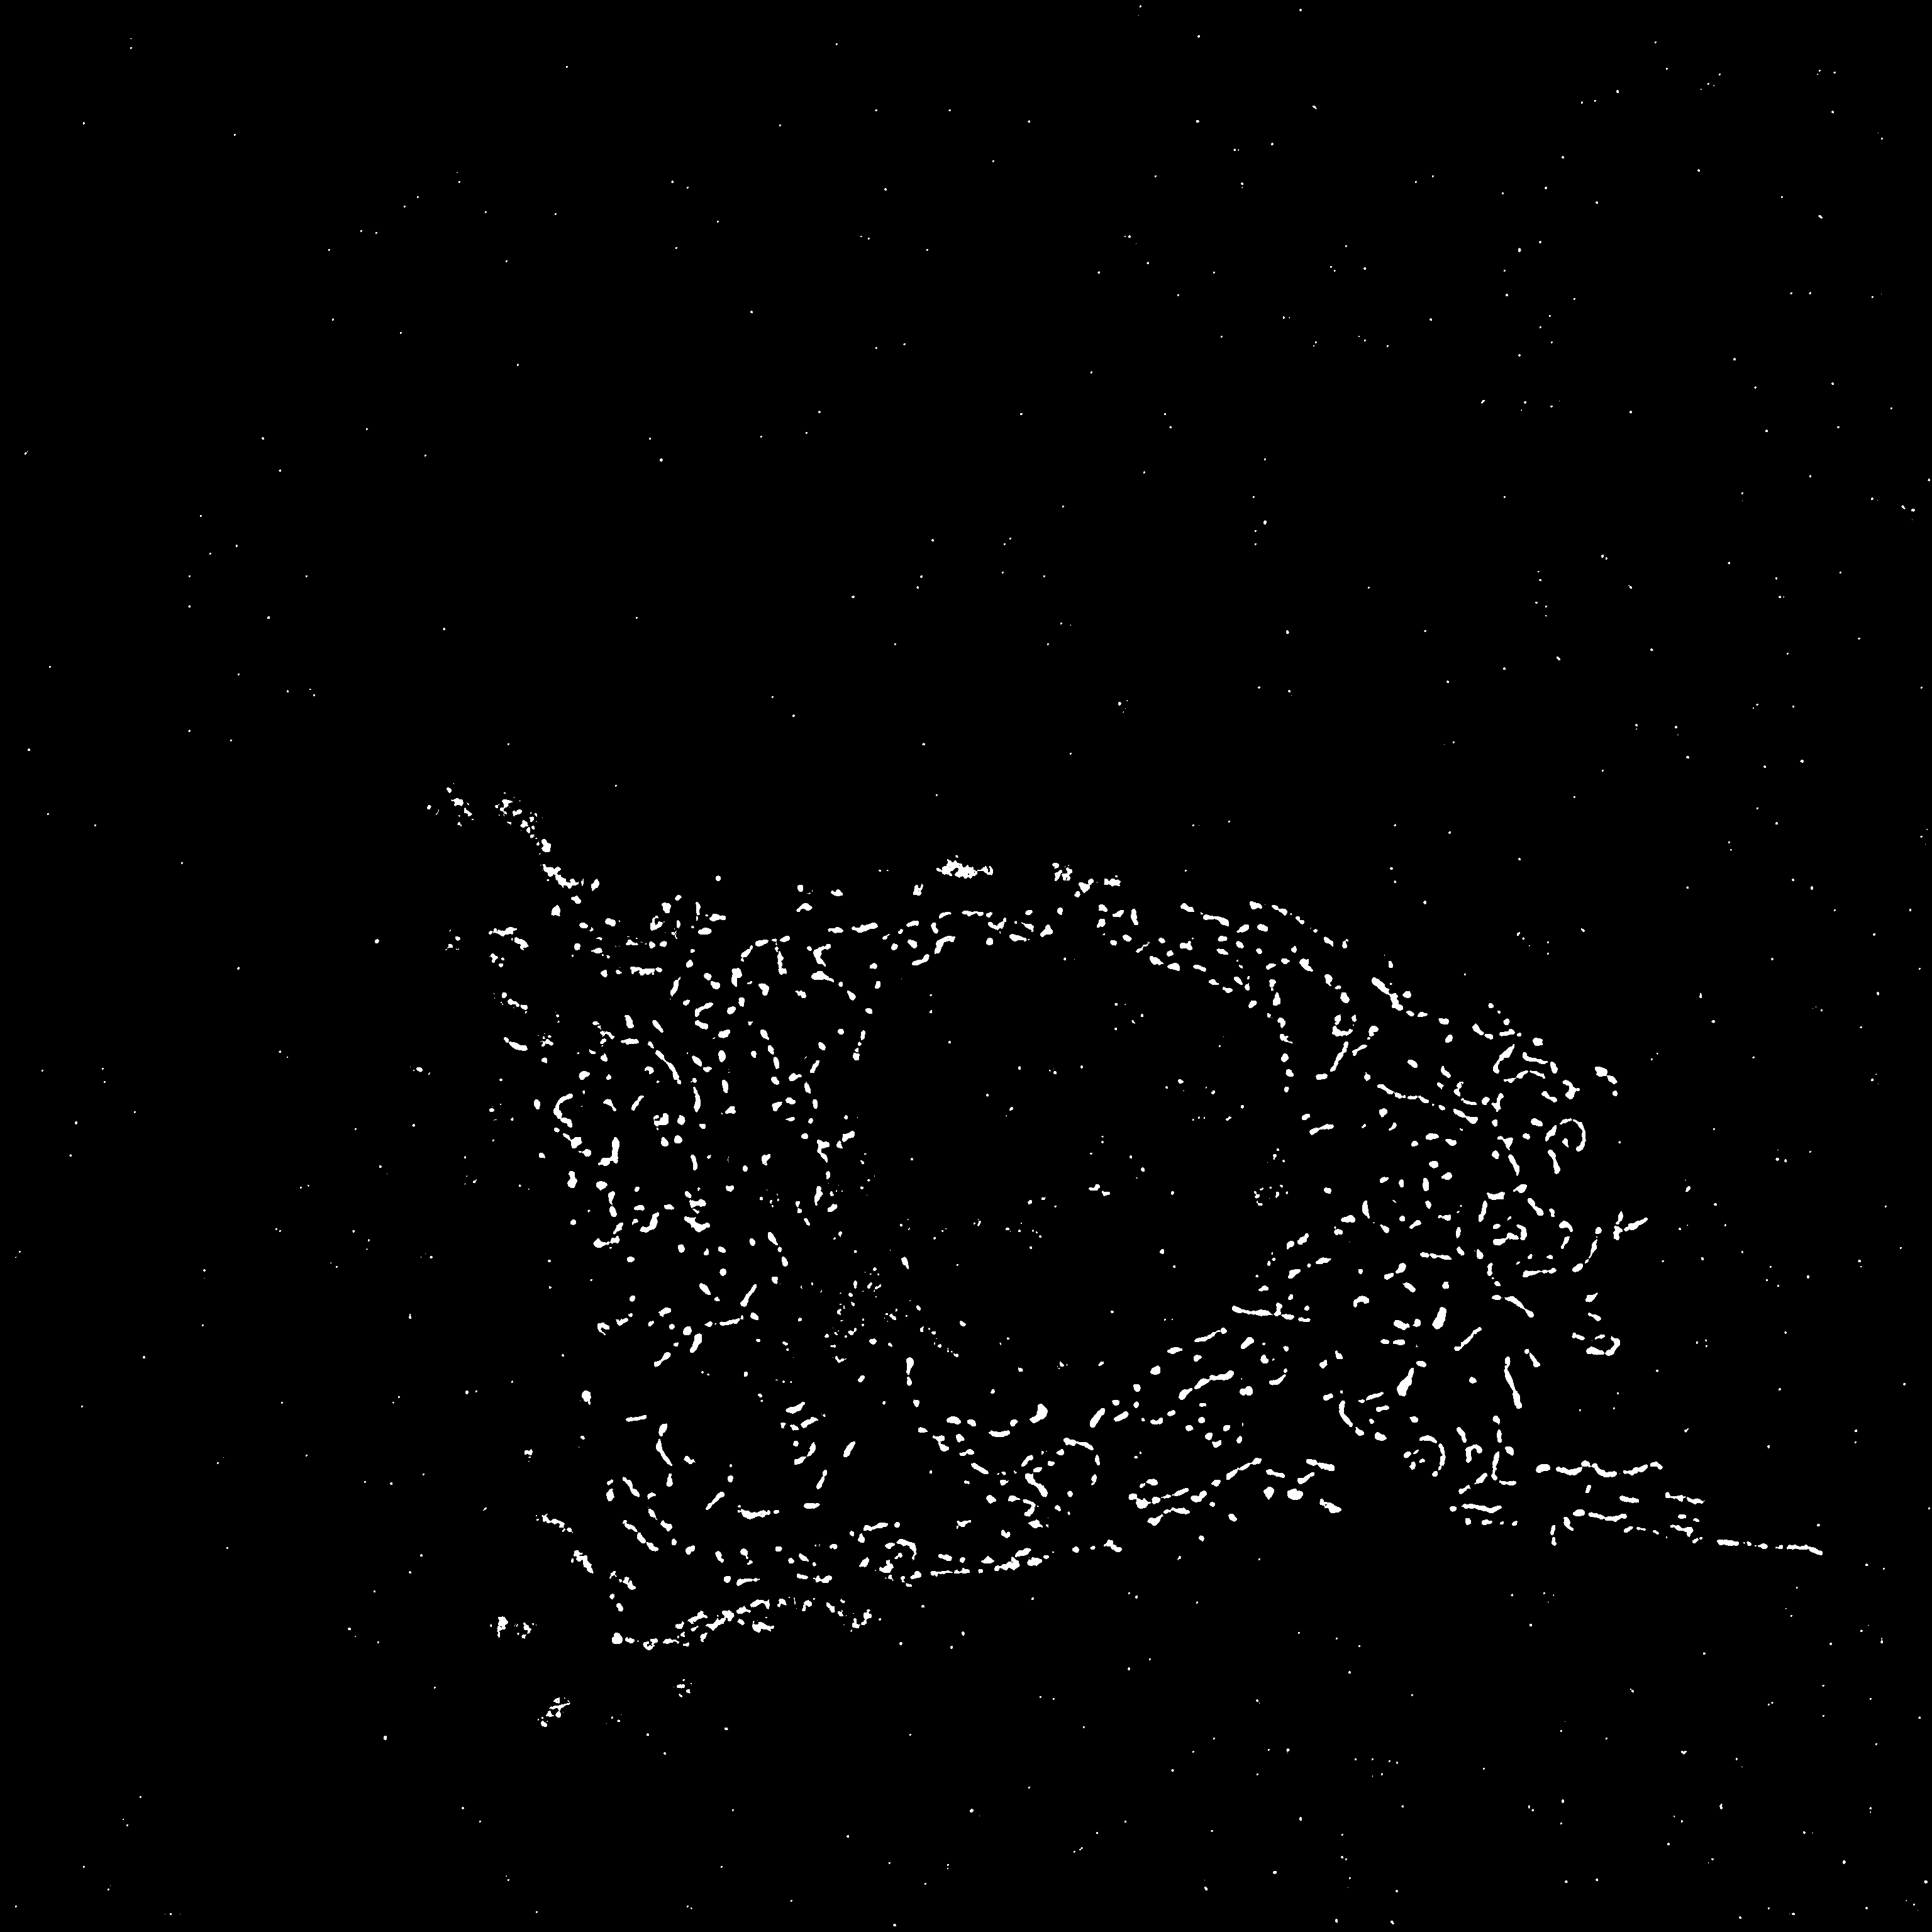
\includegraphics[width=0.3\textwidth]{figs/ch4figs/image_shortlisting/local/Bernsen_p10_w15_CCCP_1C=1T=0.png}}
	\subcaptionbox{Bernsen thresholding with a contrast threshold of 15\label{subfig:bern_15}}{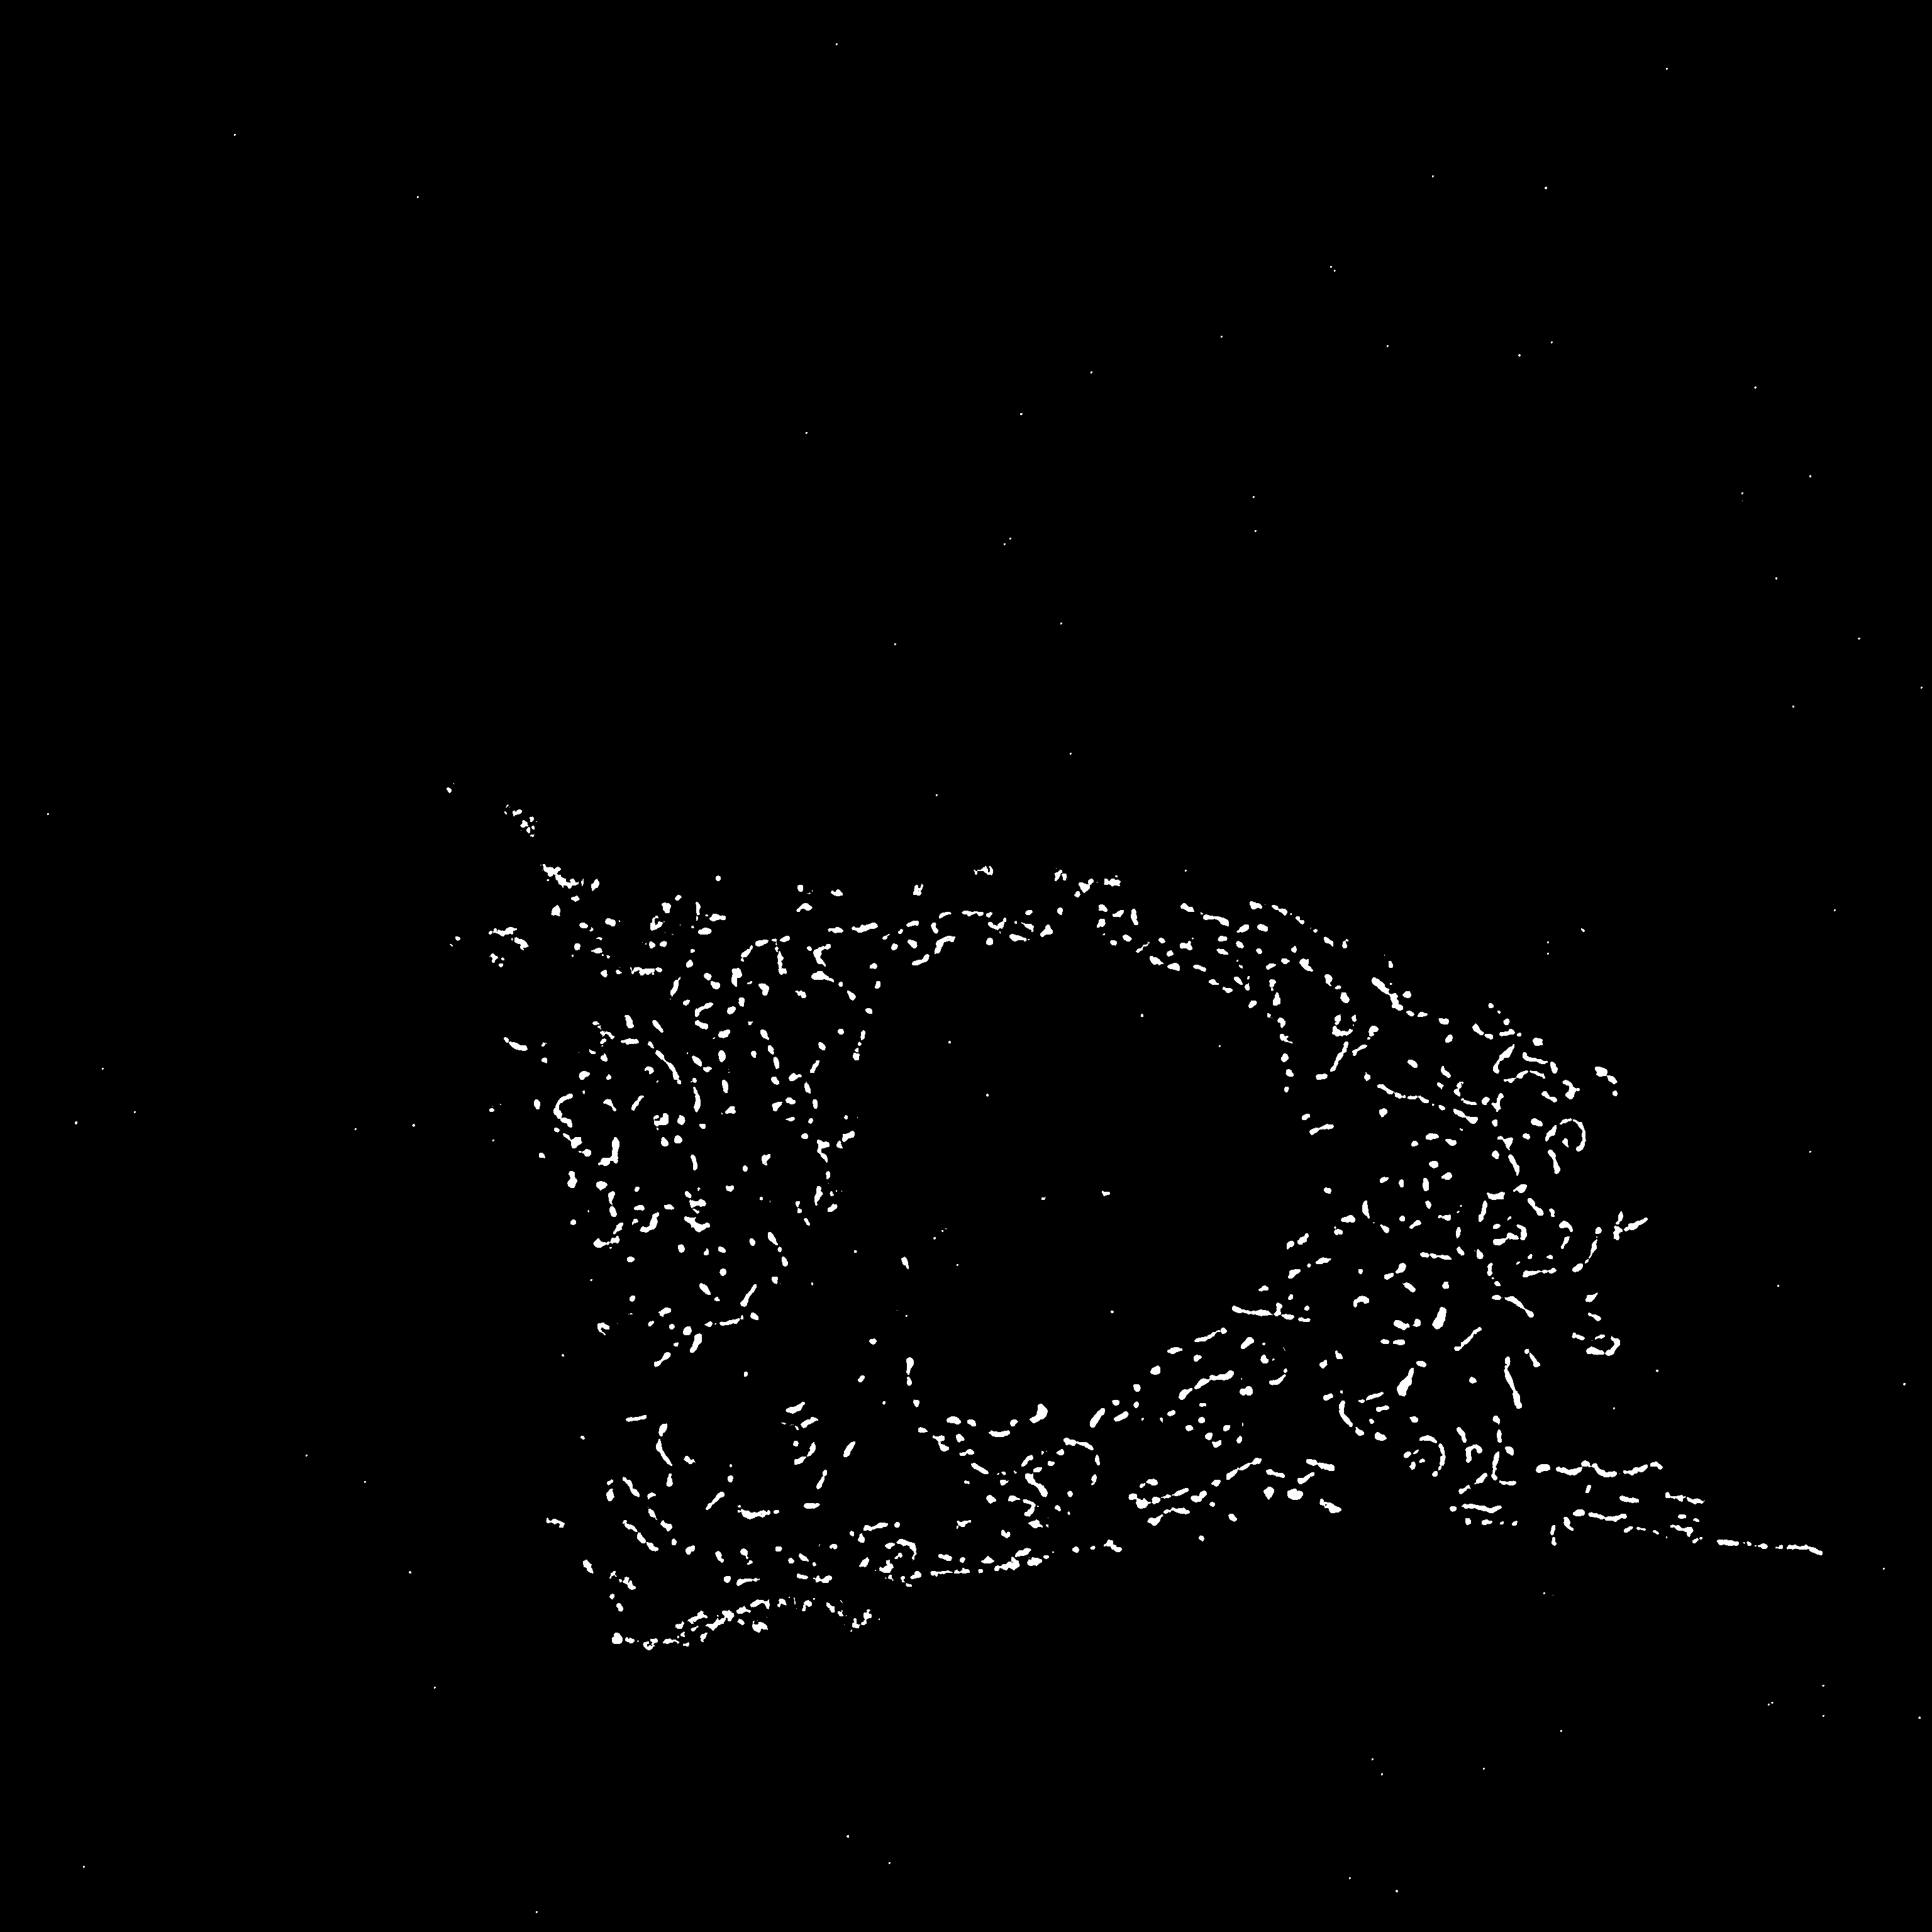
\includegraphics[width=0.3\textwidth]{figs/ch4figs/image_shortlisting/local/Bernsen_p15_w15_CCCP_1C=1T=0.png}}
	\subcaptionbox{Bernsen thresholding with a contrast threshold of 20\label{subfig:bern_20}}{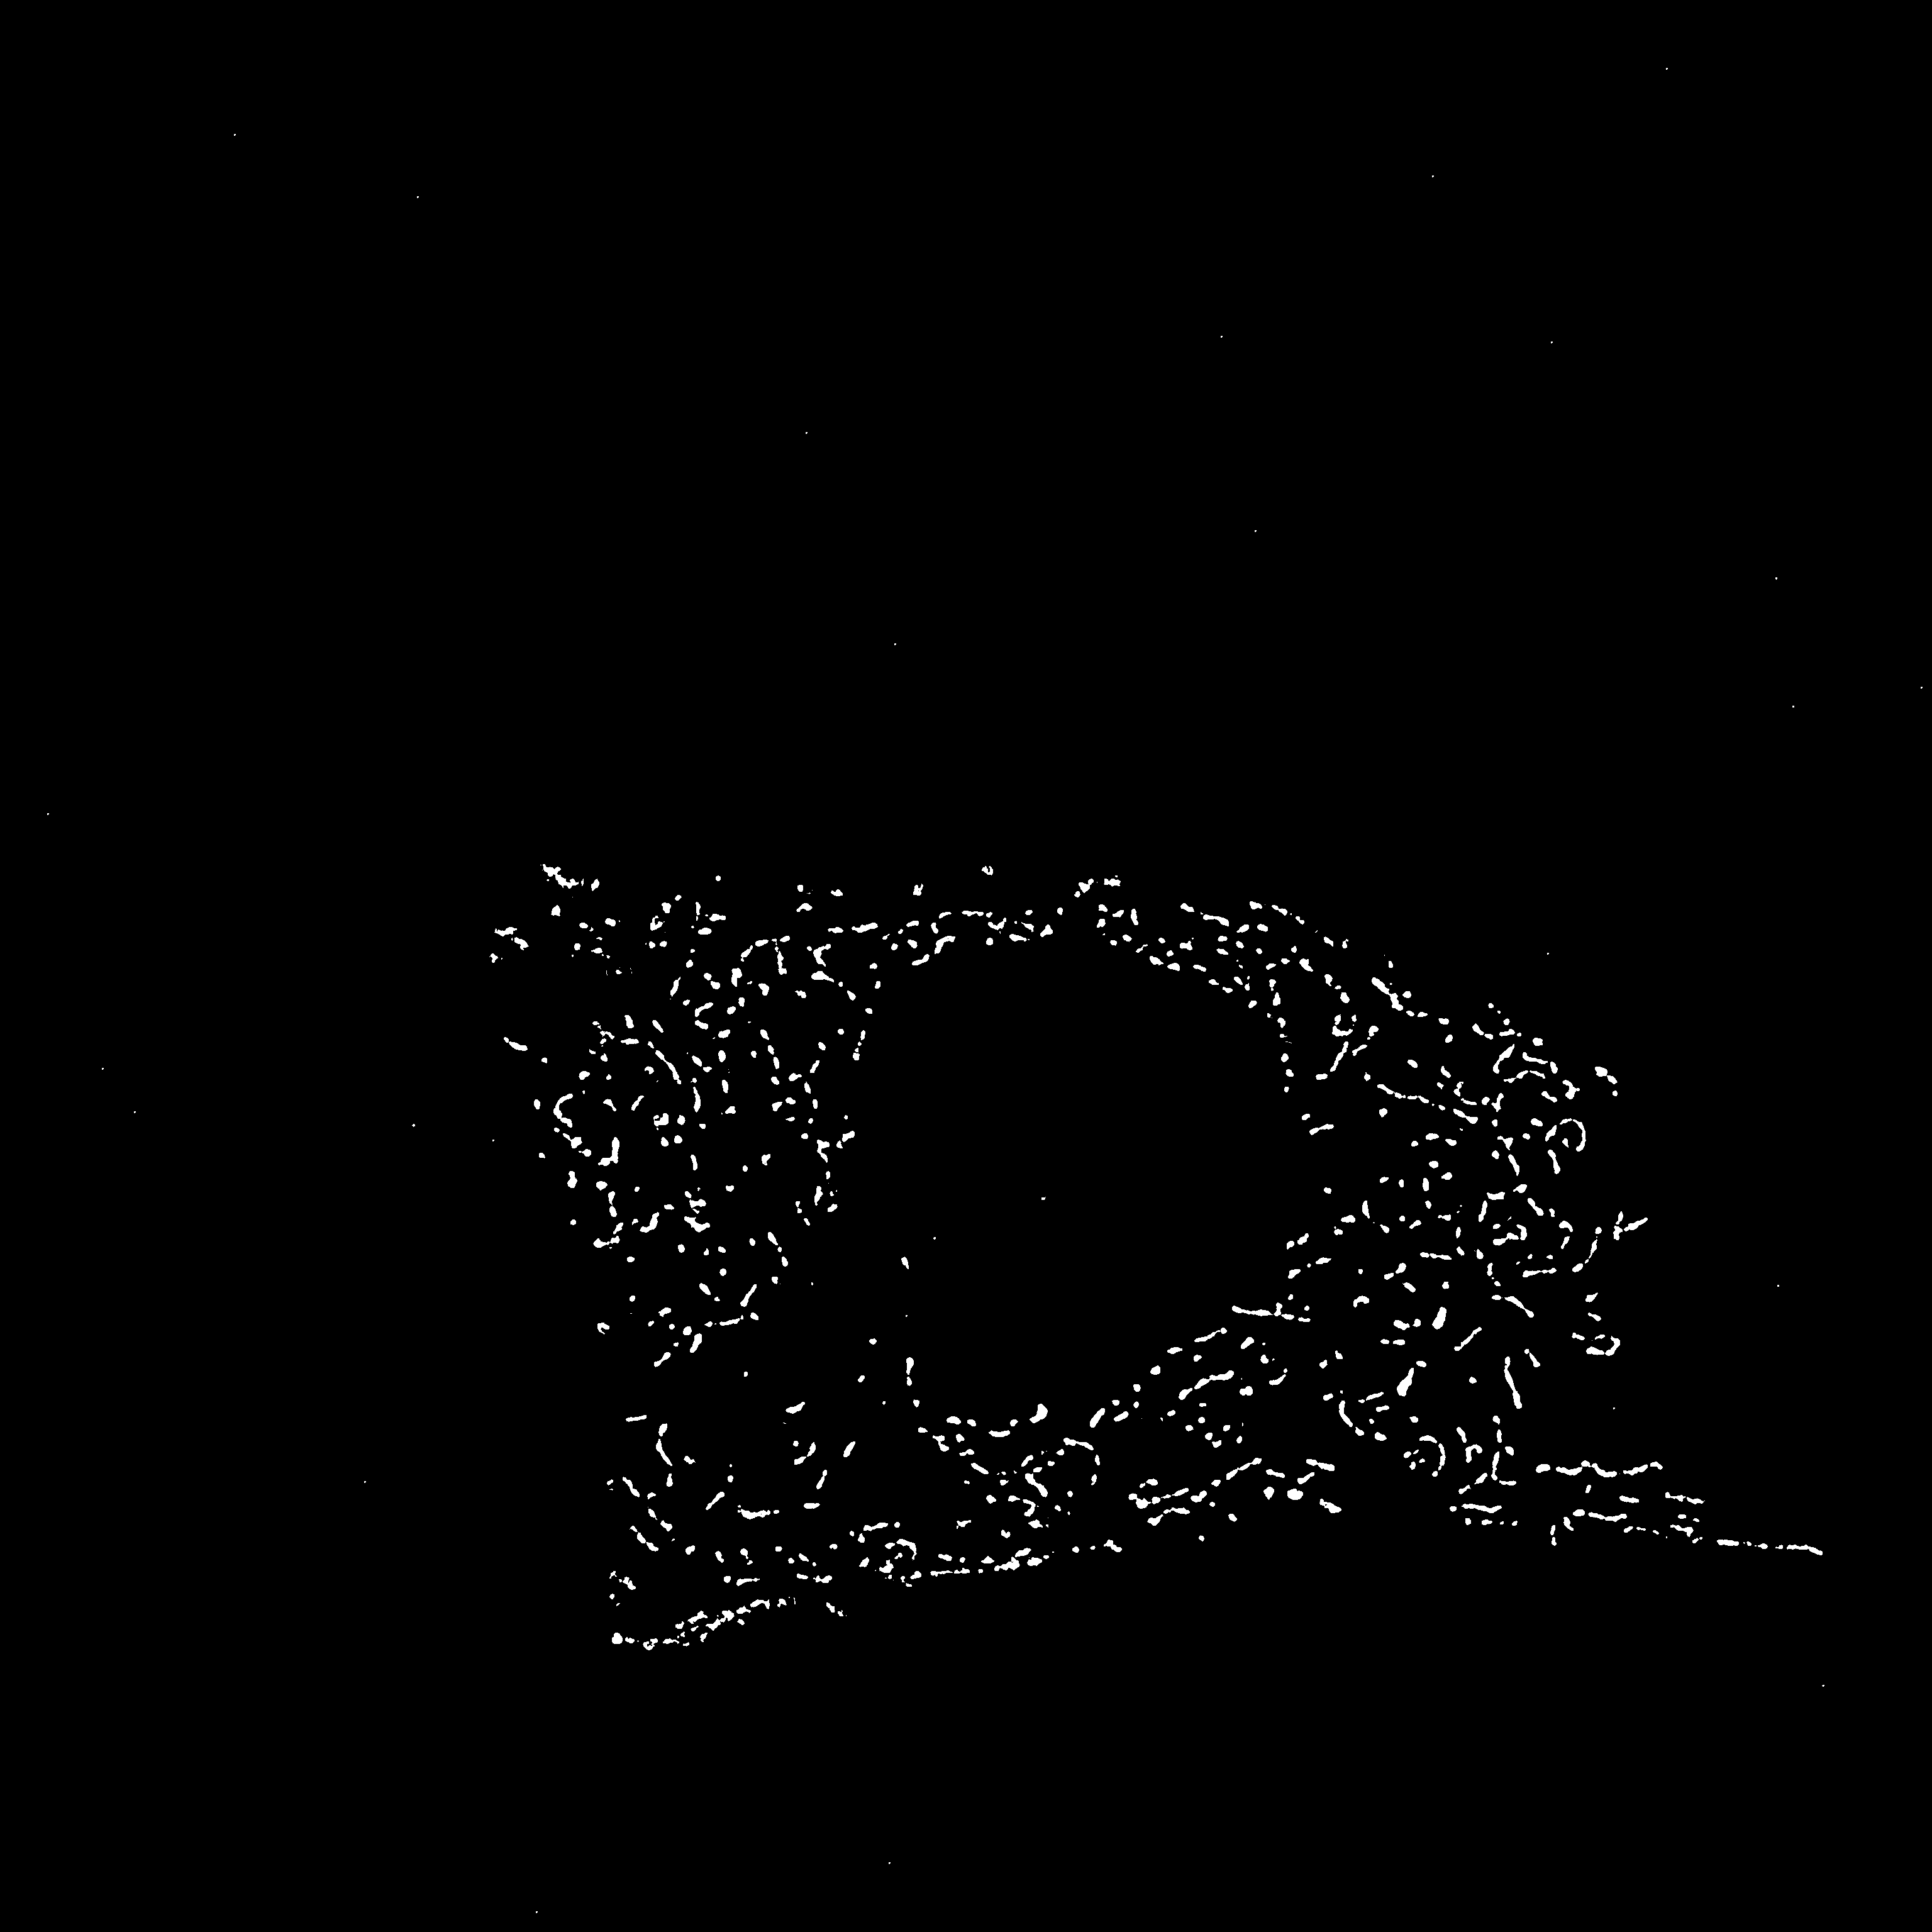
\includegraphics[width=0.3\textwidth]{figs/ch4figs/image_shortlisting/local/Bernsen_p20_w15_CCCP_1C=1T=0.png}}
	\subcaptionbox{MidGrey thresholding with a subtraction constant of -5\label{subfig:midG_-5}}{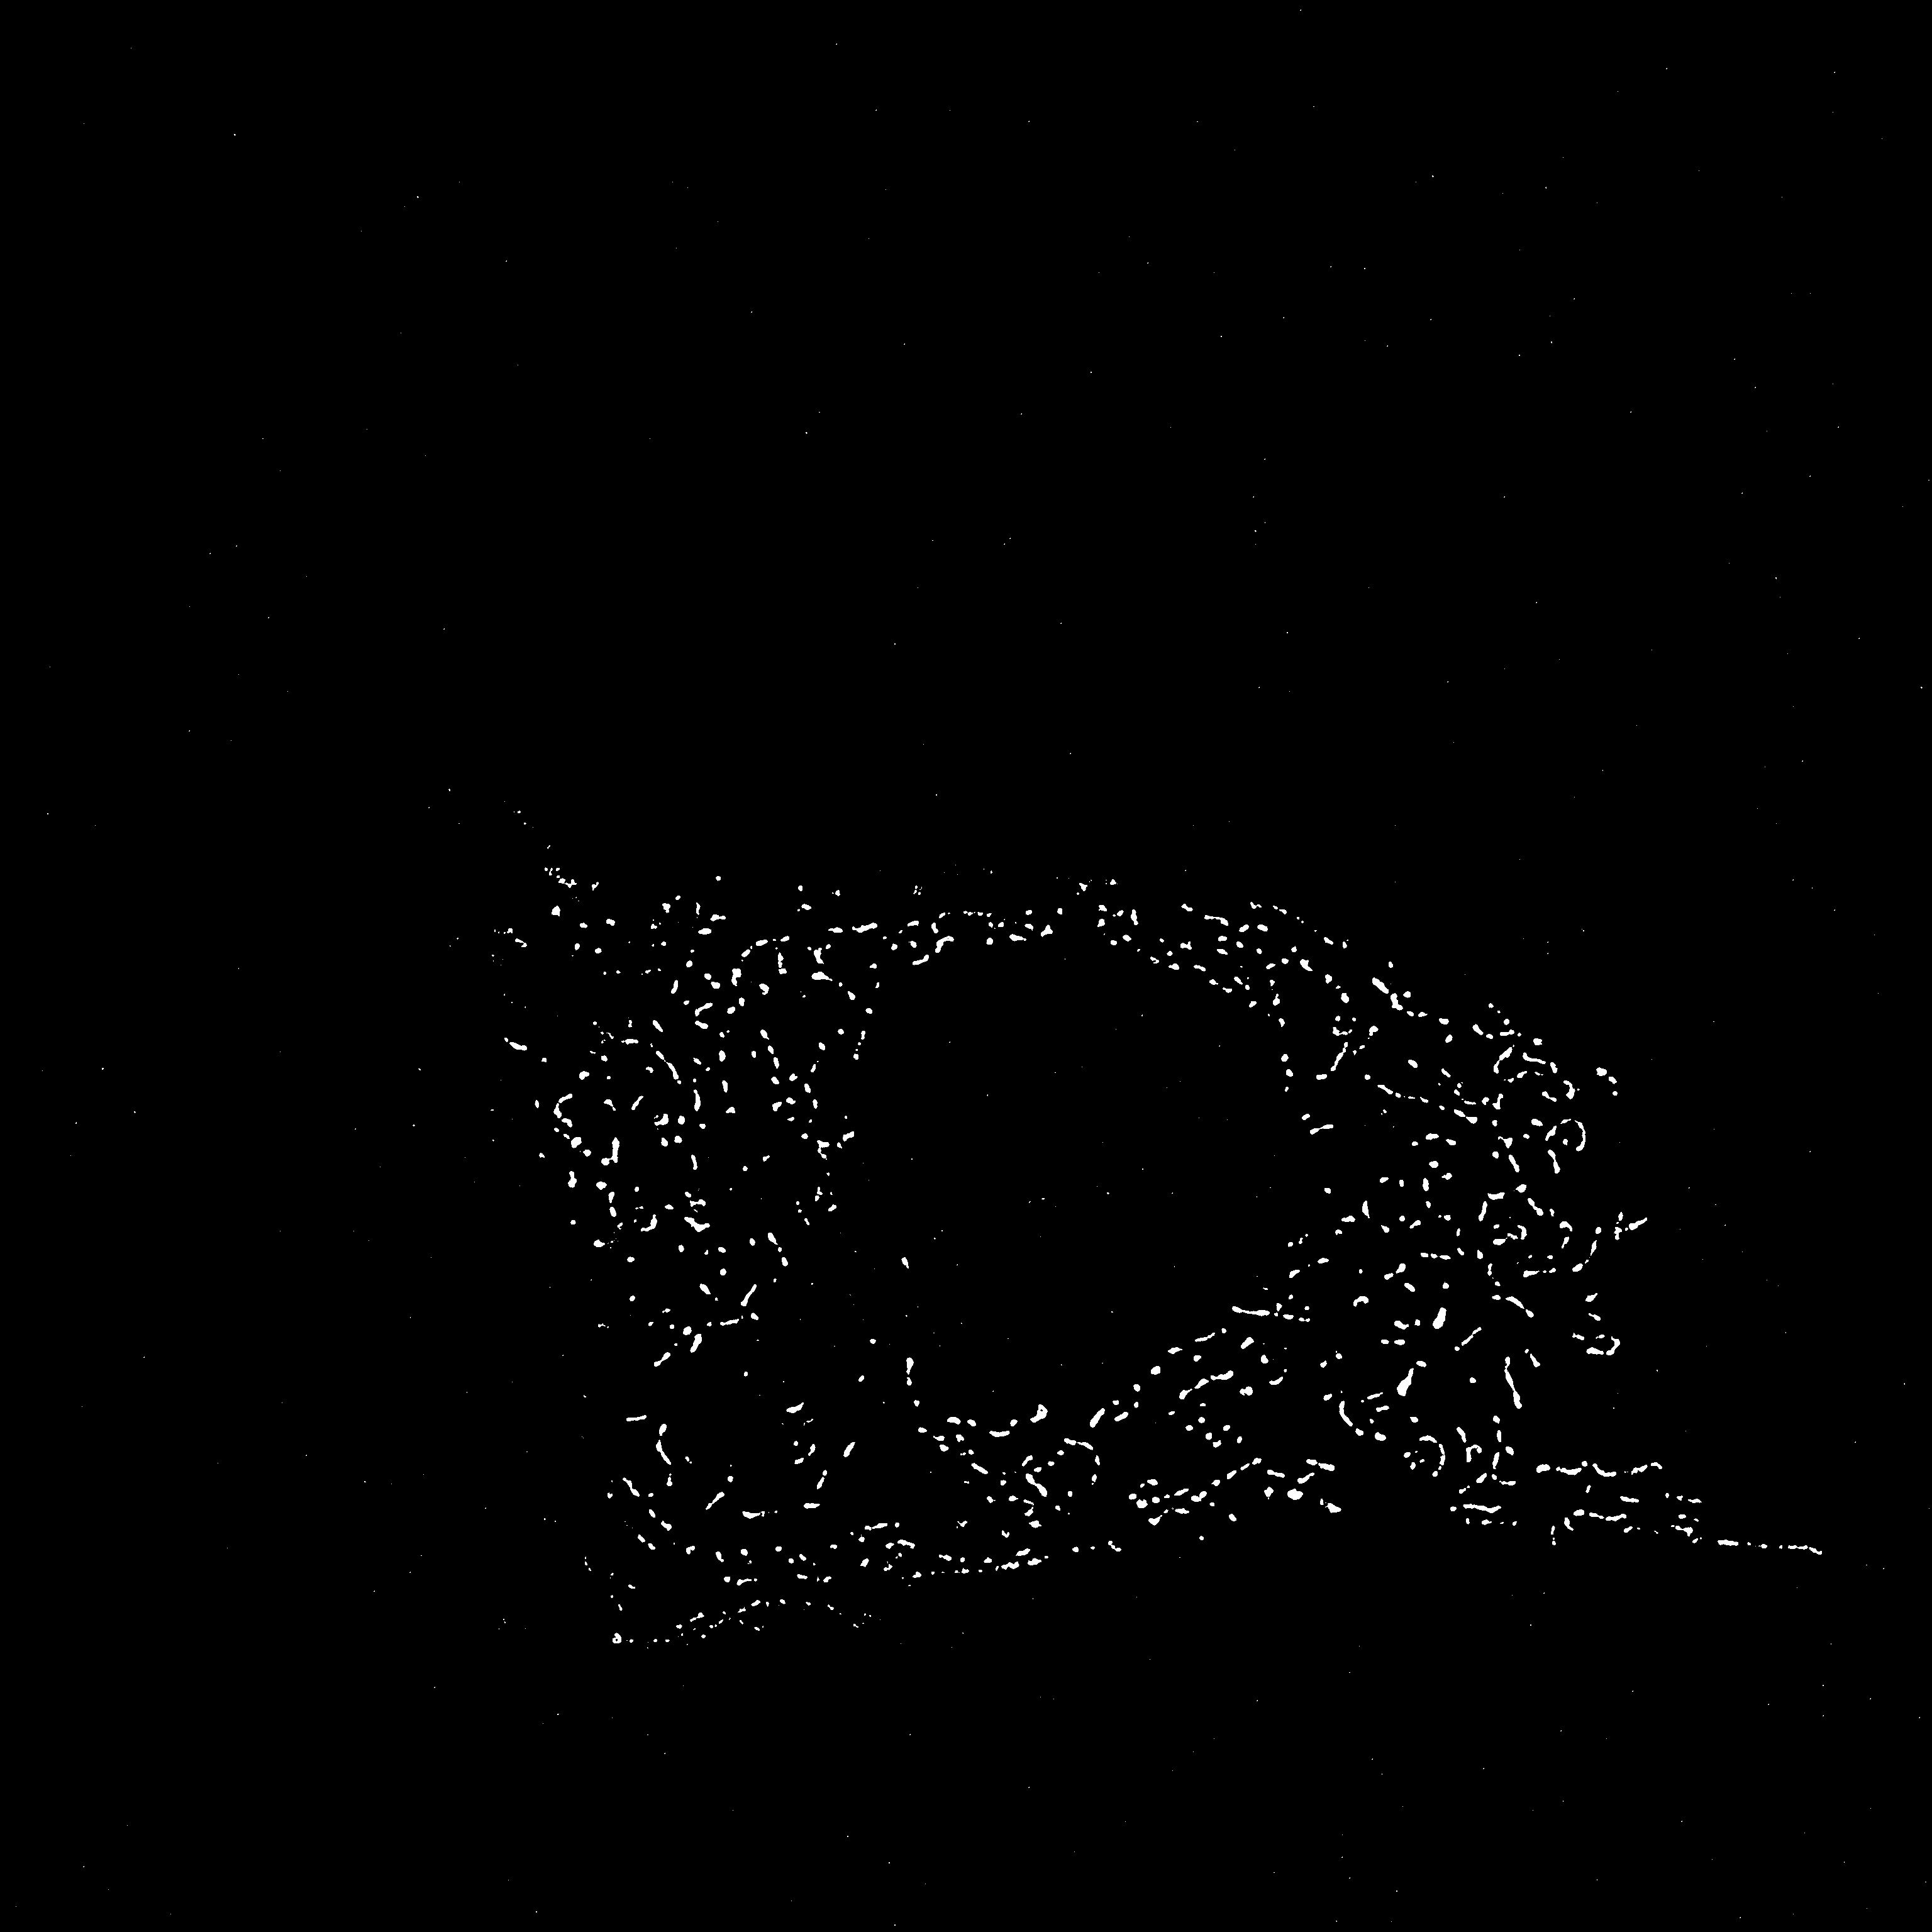
\includegraphics[width=0.3\textwidth]{figs/ch4figs/image_shortlisting/local/MidGrey_p-5_w15_CCCP_1C=1T=0.png}}
	\subcaptionbox{MidGrey thresholding with a subtraction constant of 0\label{subfig:midG_0}}{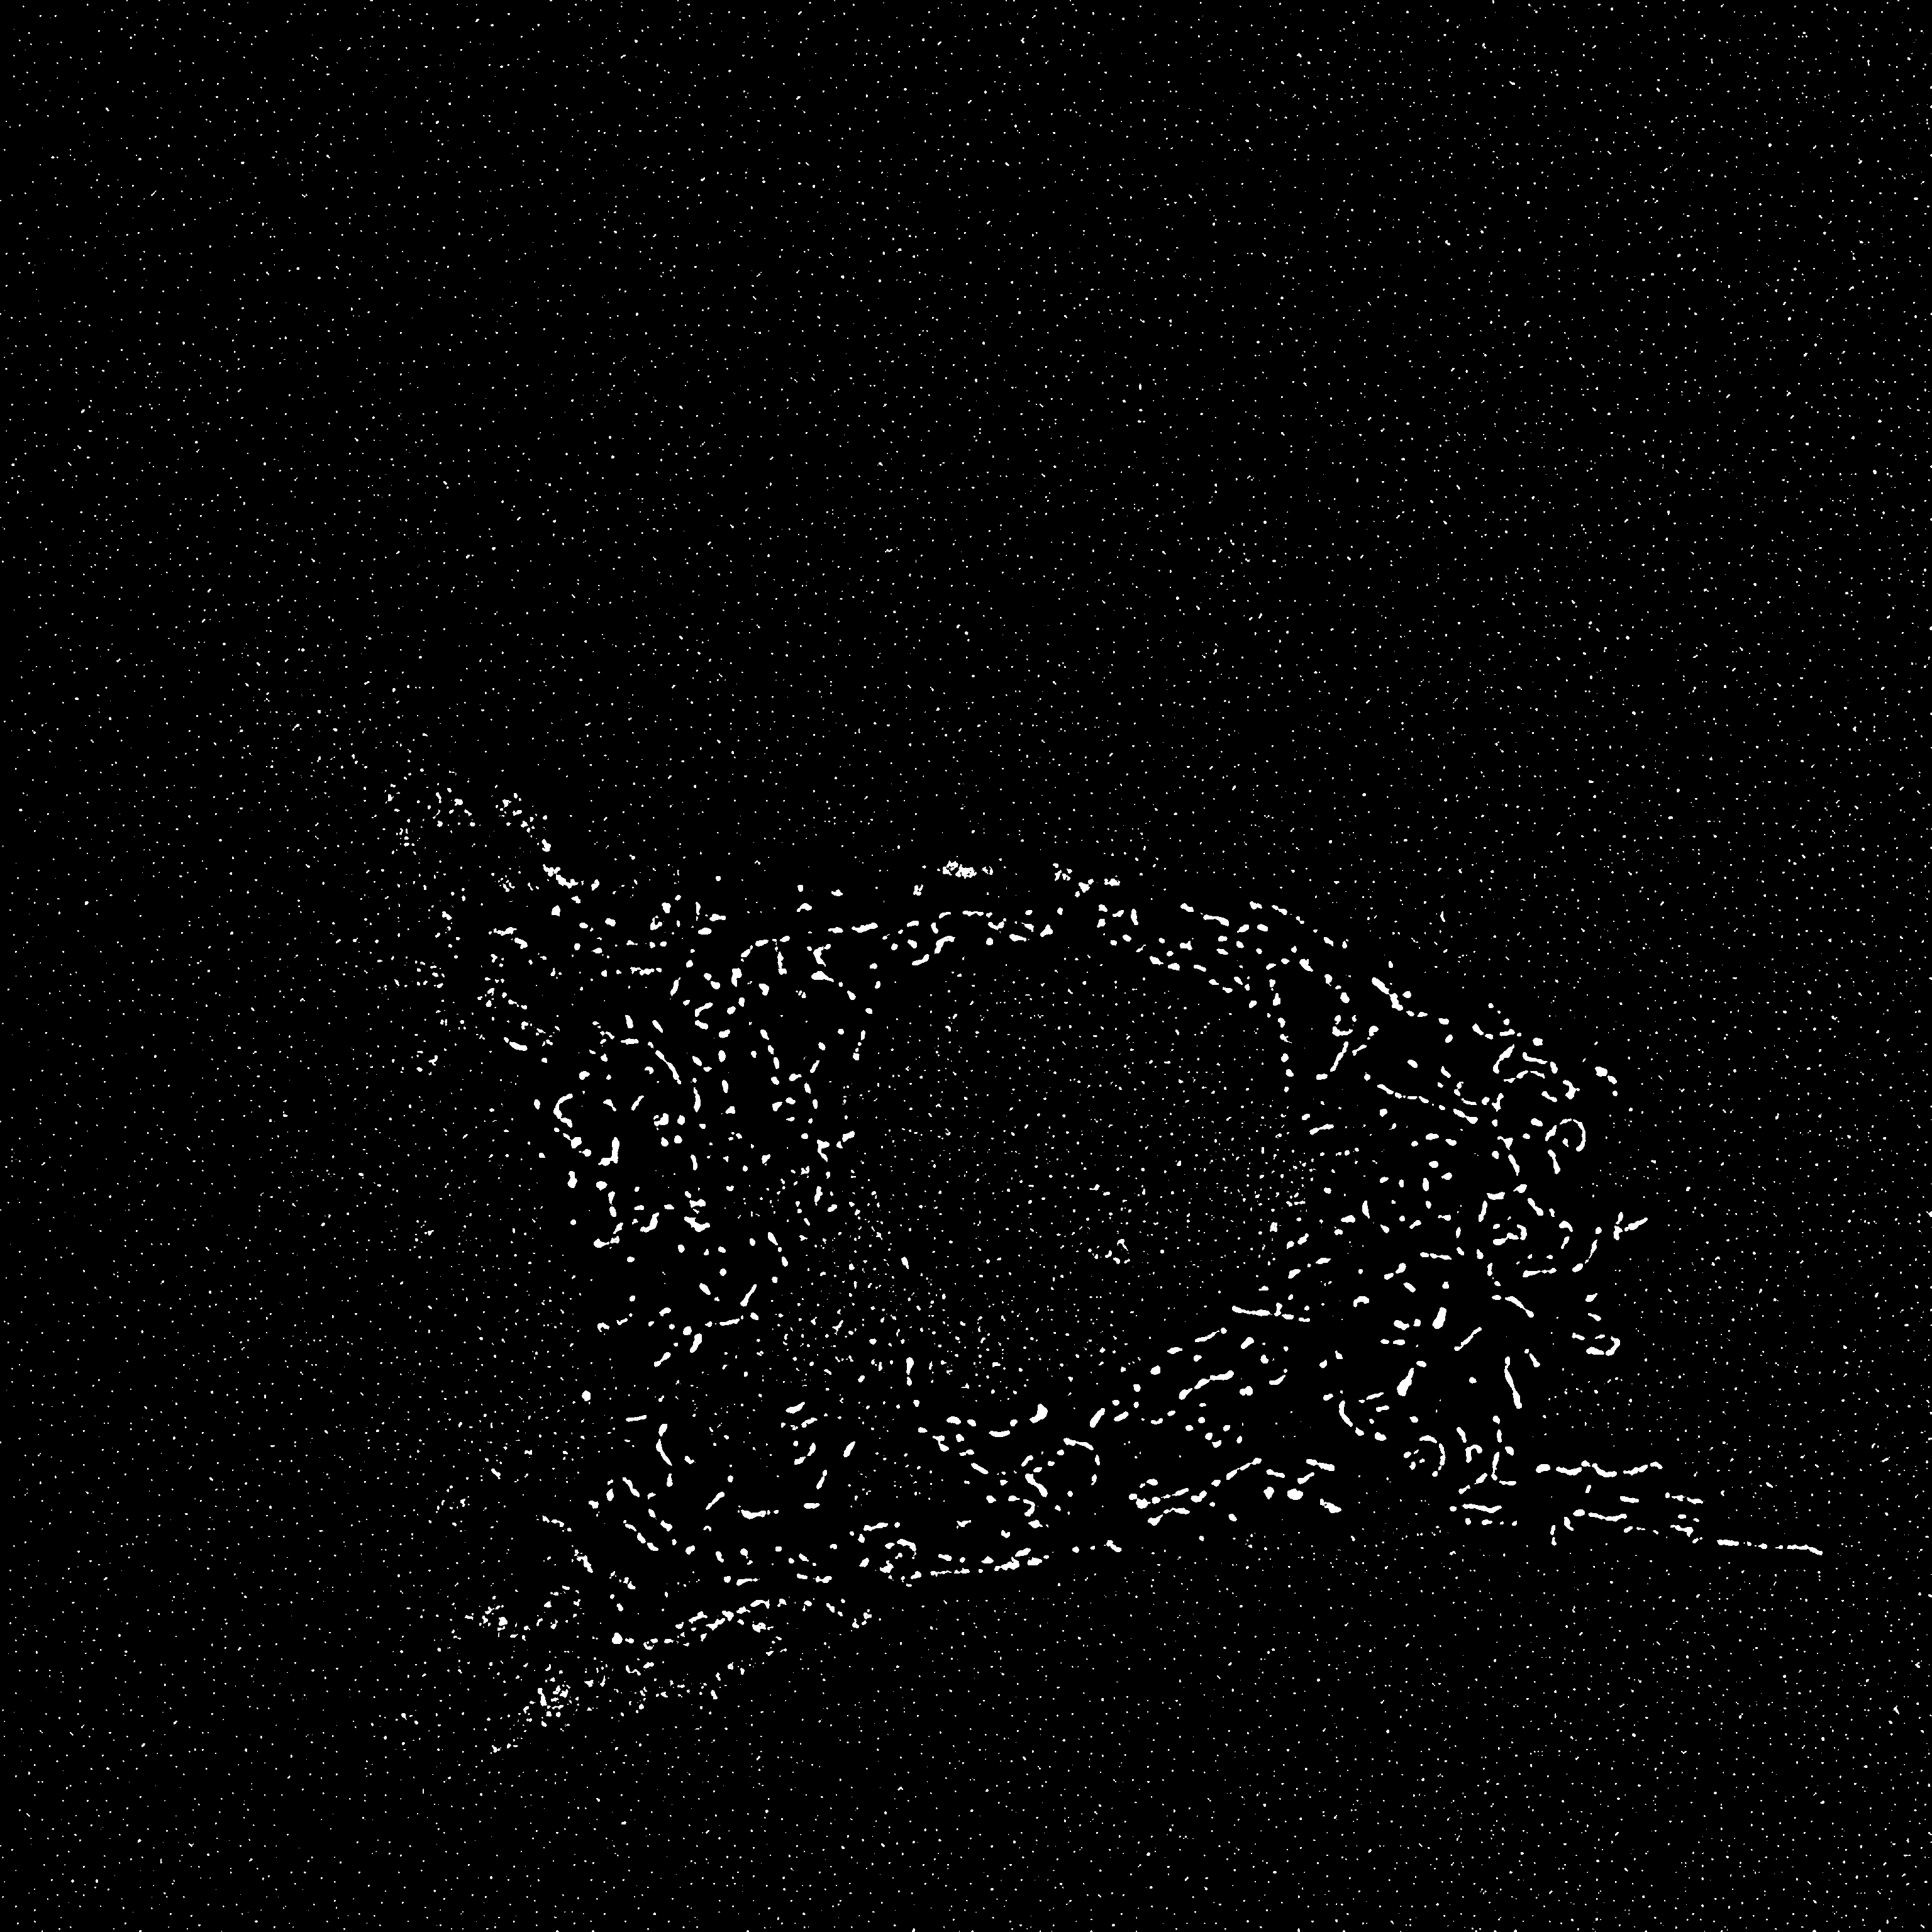
\includegraphics[width=0.3\textwidth]{figs/ch4figs/image_shortlisting/local/MidGrey_p0_w15_CCCP_1C=1T=0.png}}
	\subcaptionbox{MidGrey thresholding with a subtraction constant of 5\label{subfig:midG_5}}{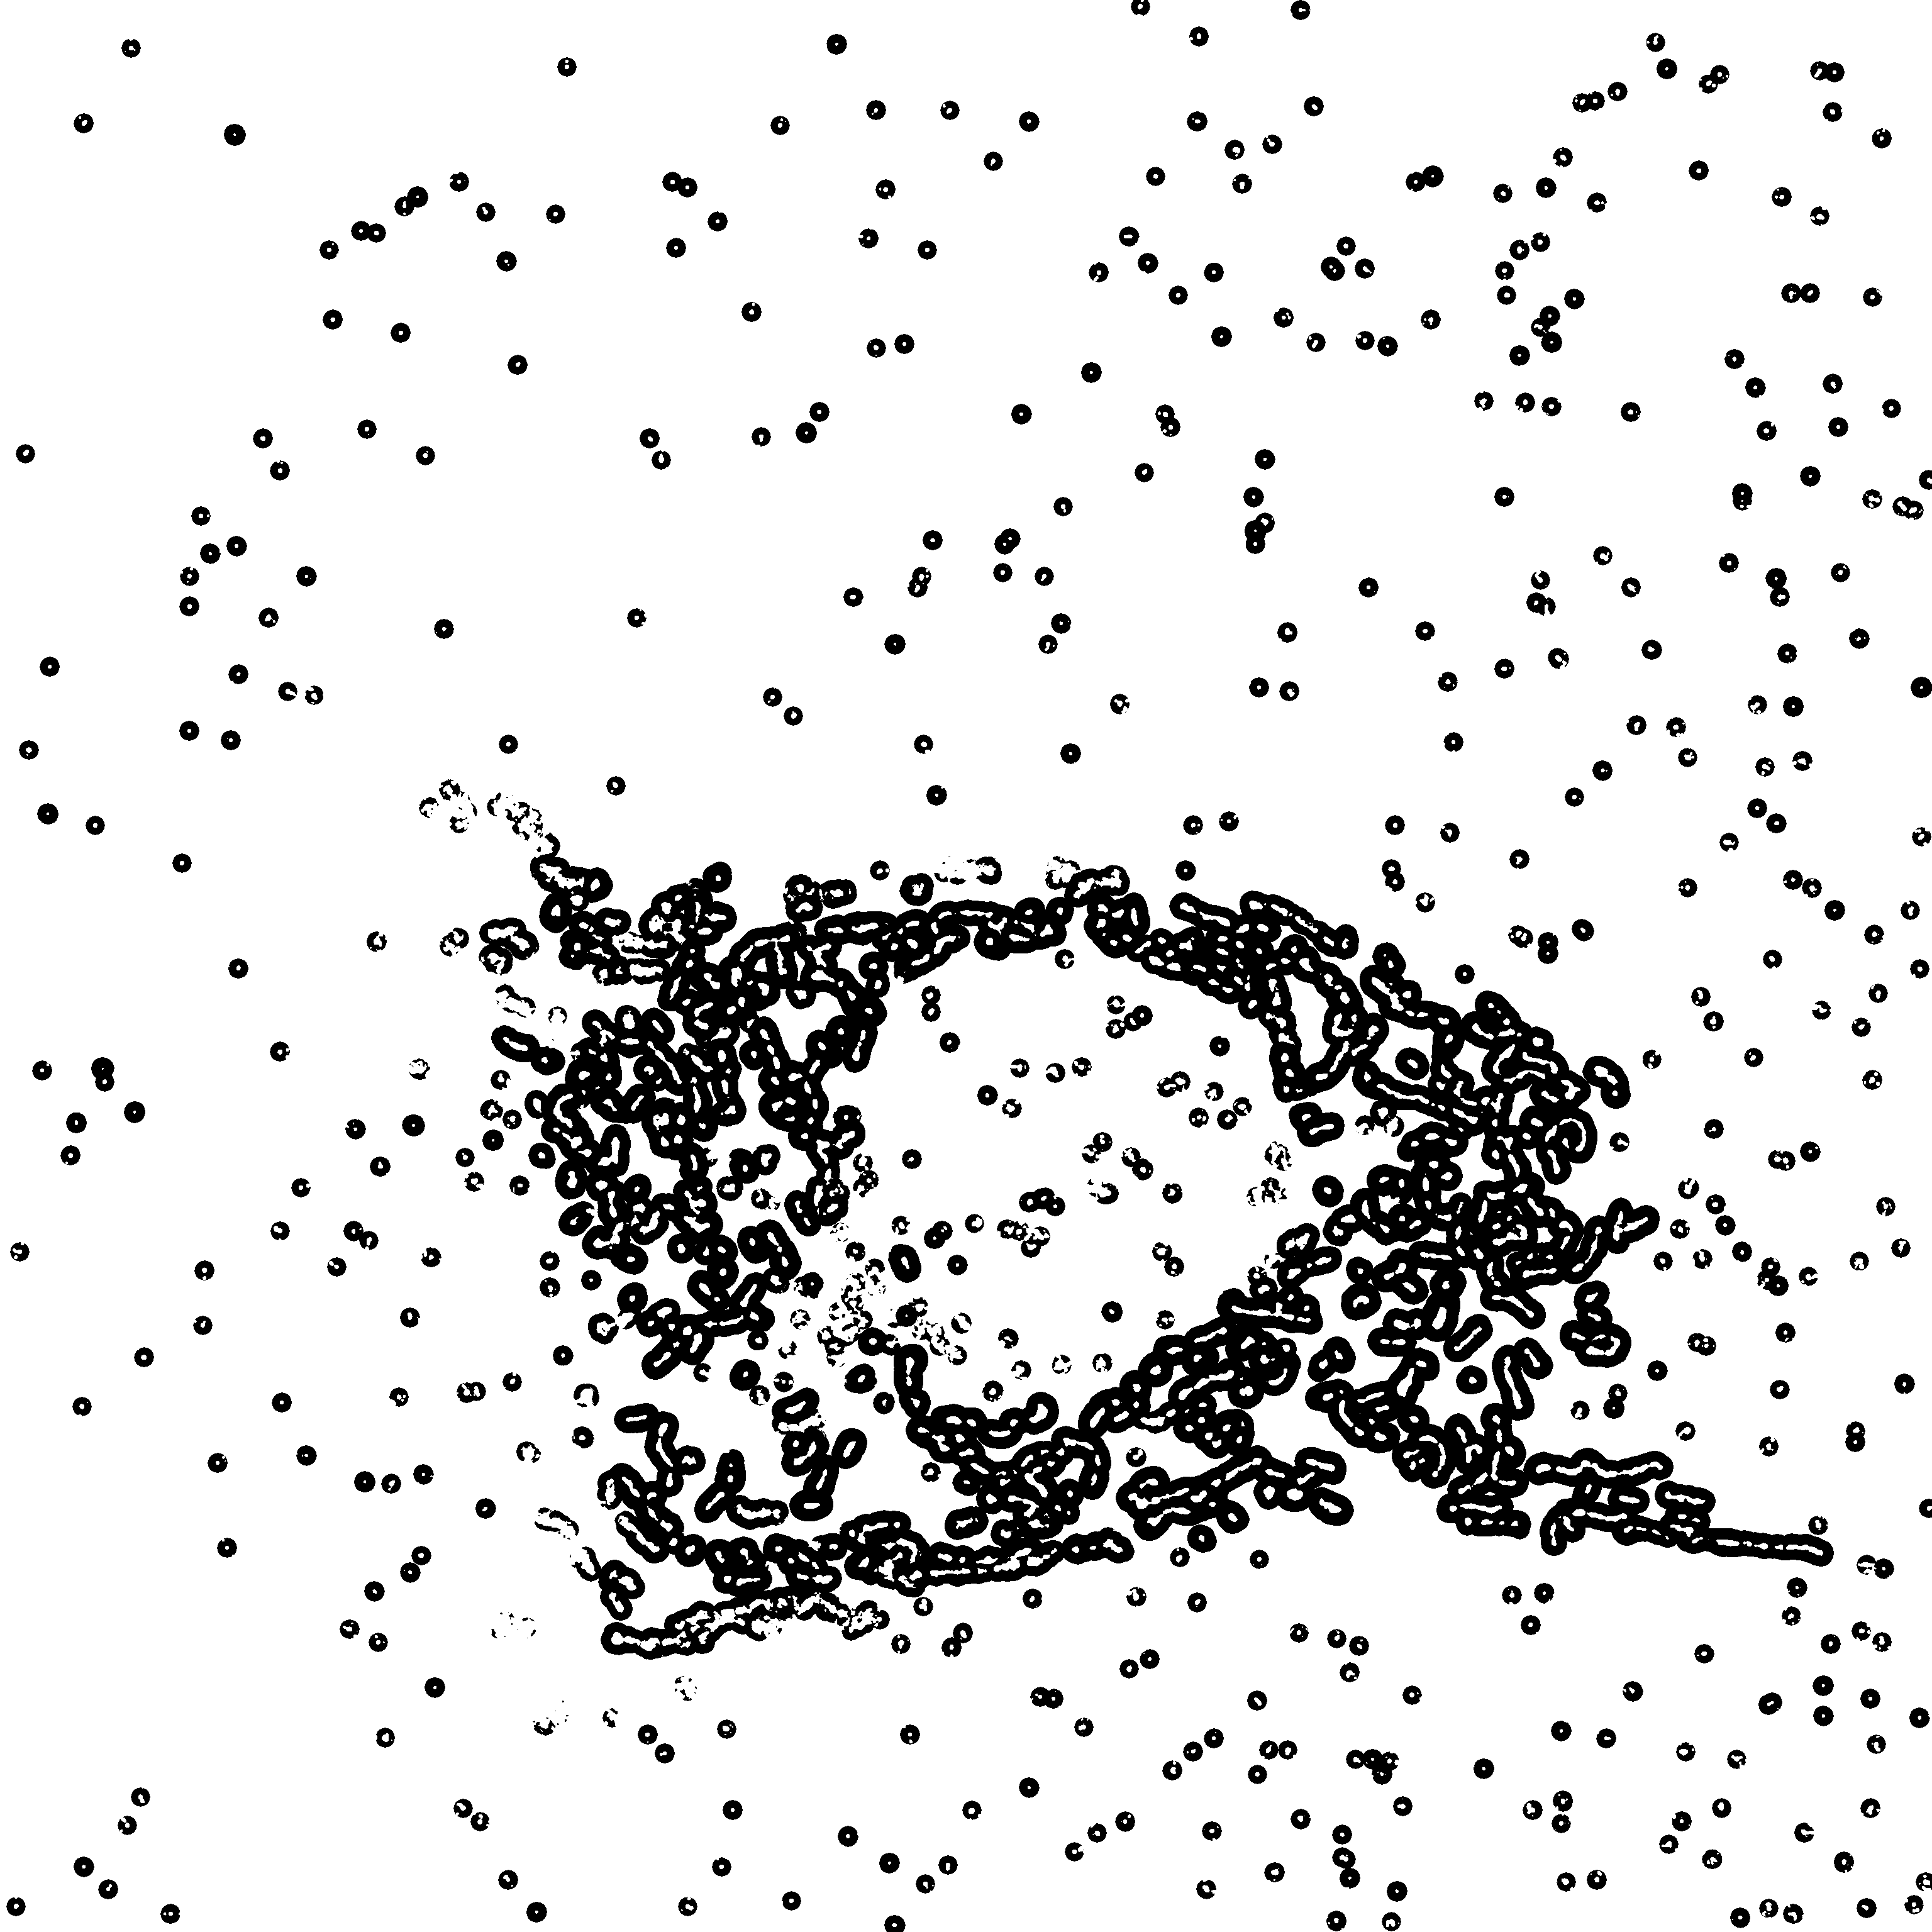
\includegraphics[width=0.3\textwidth]{figs/ch4figs/image_shortlisting/local/MidGrey_p5_w15_CCCP_1C=1T=0.png}}
	\caption[Showcase of the impact secondary parameter tuning can have on local thresholding methods.]{Showcase of the impact secondary parameter tuning can have on local thresholding methods. Bernsen and MidGrey are used in this showcase with both being applied to sample 1.}
	\label{fig:local_param_tuning}
\end{figure}

\clearpage
\section{Visual analysis}\label{sec:visual_analysis}
The visual analysis of the thresholding methods will be performed by comparing the binarised results to the original intensity sample images and a thresholding baseline. The methods that are to be explored are AHT, the method developed throughout this project, and the global and local thresholding methods that have been selected through the previous shortlisting process. The binarisation baselines are produced through Hysteresis thresholding, which involves the manual selection of low and high thresholds, with this method being chosen due to the AHT method, the focus of these evaluations, also implementing Hysteresis thresholding. The manual selection of the high and low thresholds for this Hysteresis threshold baseline is that the involvement of a human allows the resultant binarisation to be optimized to capture the structures of most interest in the foreground. This is achieved through prior knowledge regarding the visual characteristics (e.g. size, shape) of the structures of interest, the ability to identify out-of-focus structures, and the ability to identify degradations such as noise. This is not without detriment, though, as this human-driven optimization of the binarisation will inject bias; thus, the baseline is not a ground truth, at most an approximation, as it is subjective. 

\begin{figure}
	\centering
	\subcaptionbox{Sample A}{\includegraphics[width=0.32\textwidth]{figs/ch4figs/visual_analysis/raw_samples/RGB_Con_2C=0.png}}
	\subcaptionbox{Sample B}{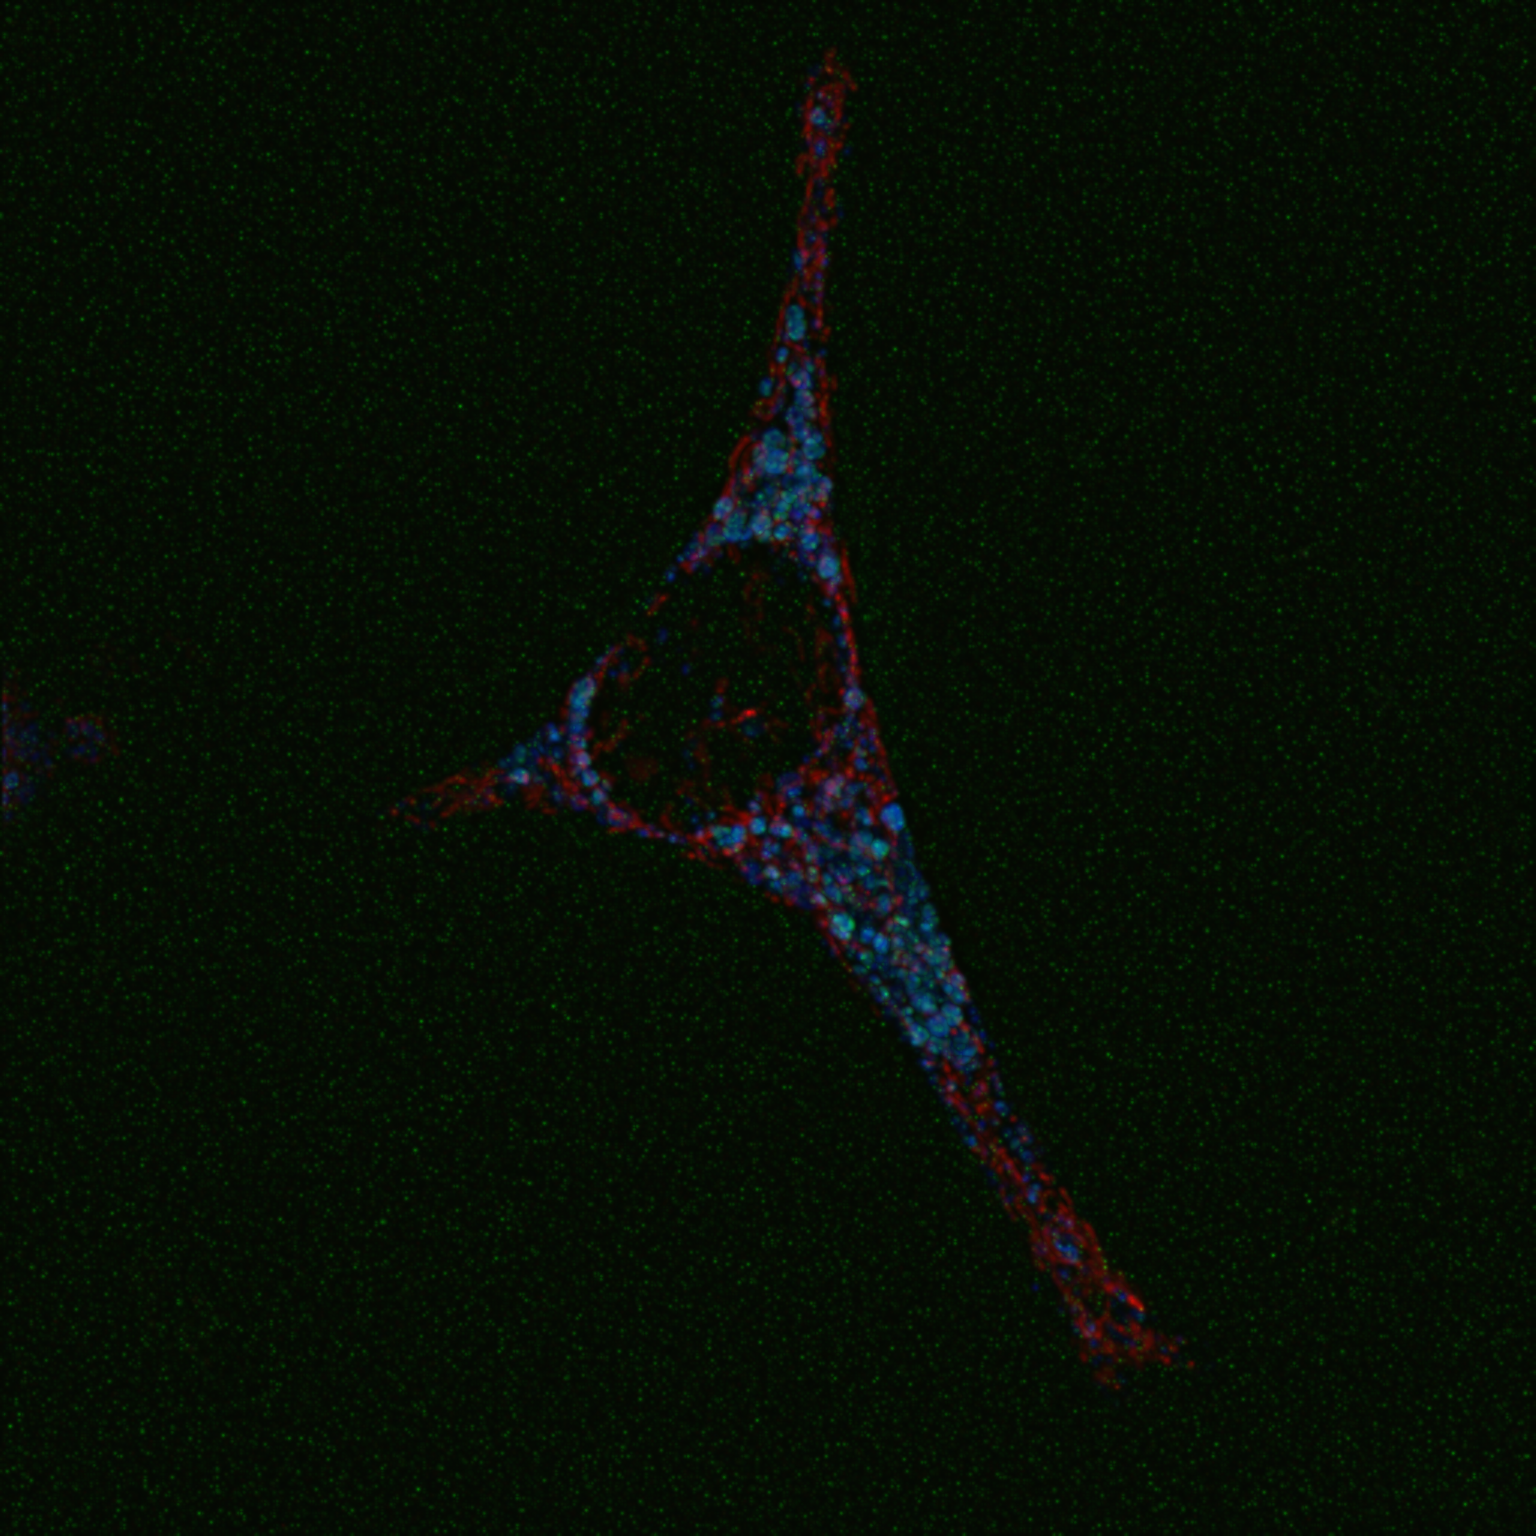
\includegraphics[width=0.32\textwidth]{figs/ch4figs/visual_analysis/raw_samples/RGB_LML_3C=0.png}}
	\subcaptionbox{Sample C}{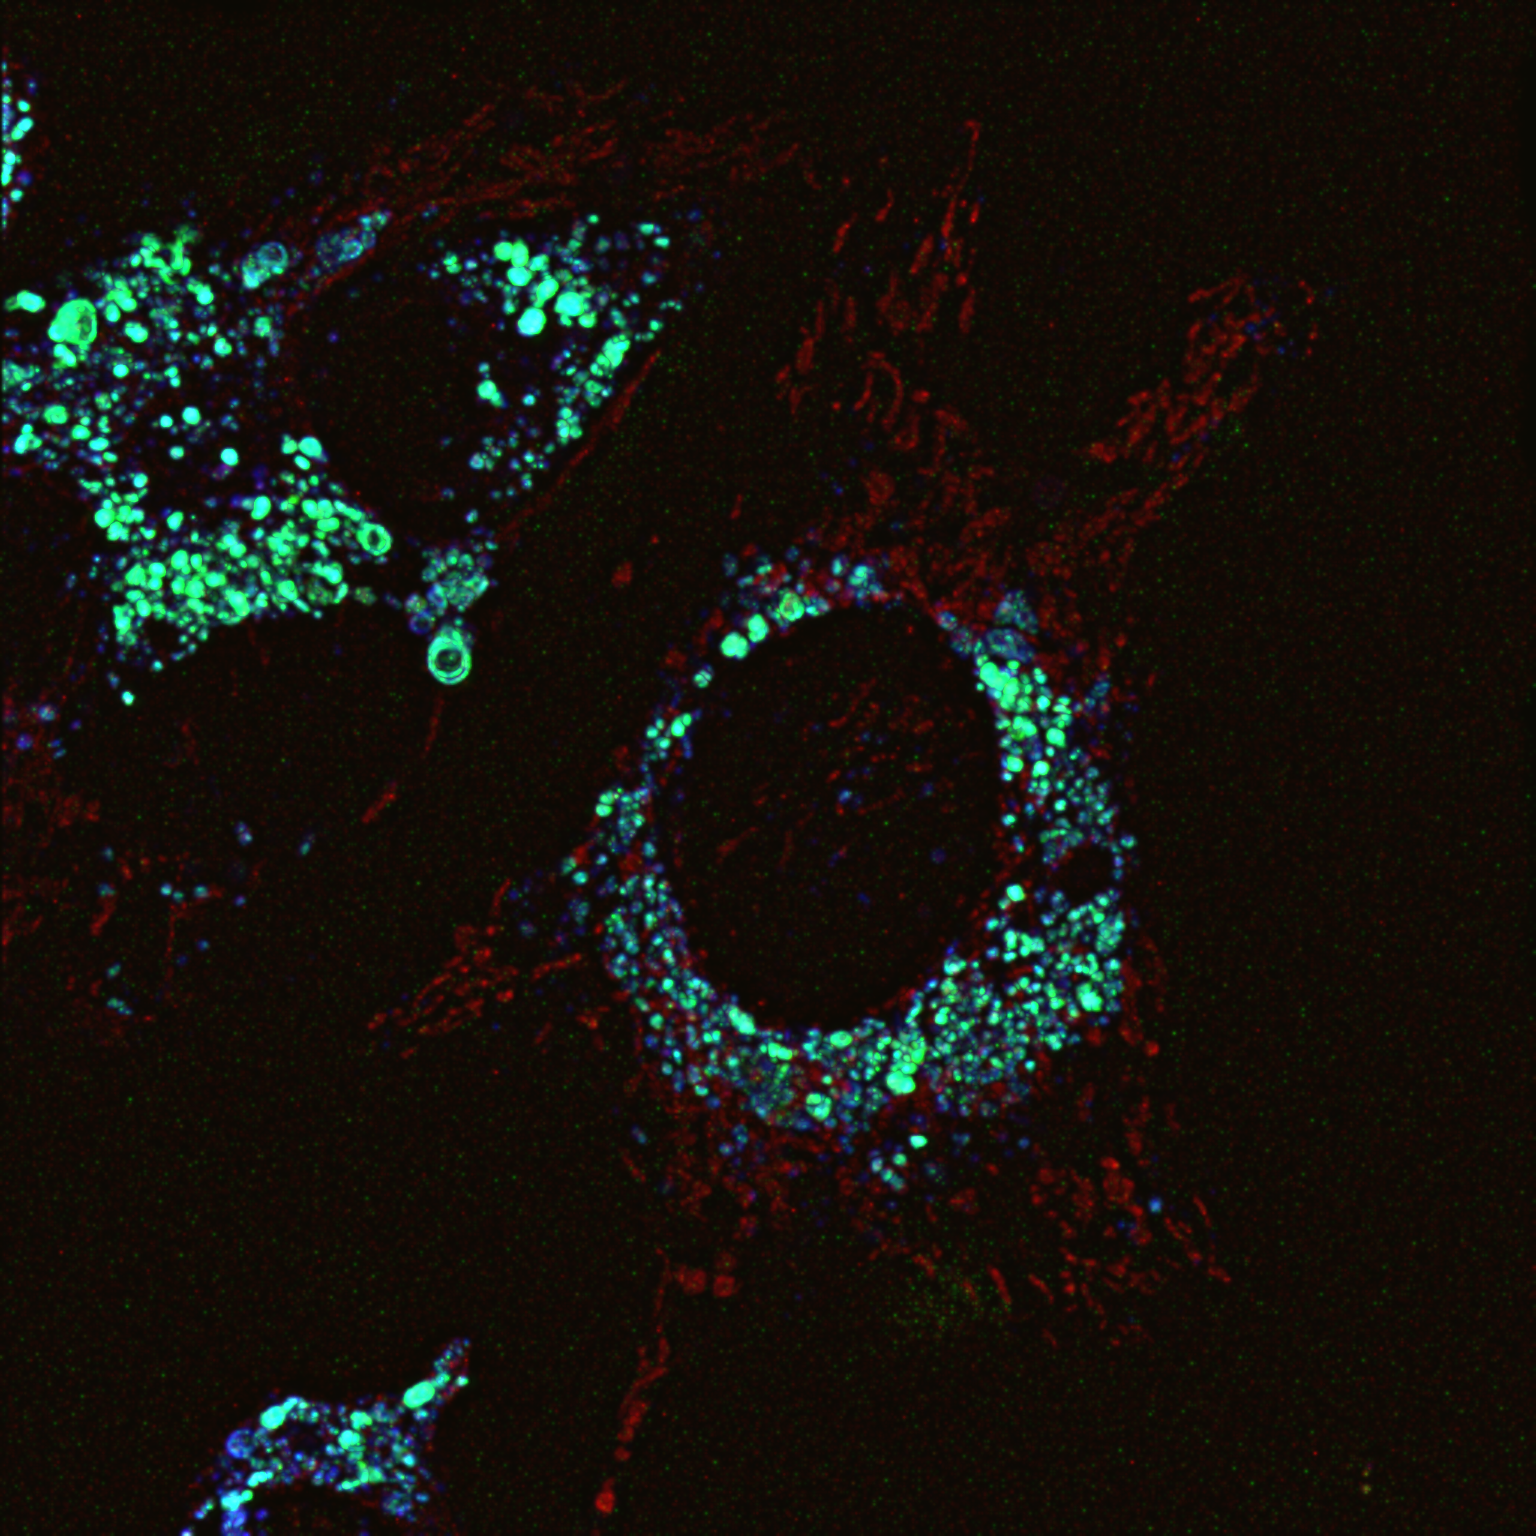
\includegraphics[width=0.32\textwidth]{figs/ch4figs/visual_analysis/raw_samples/RGB_LML_4C=1.png}}
	\caption[MIP sample images for the samples A-C where the organelle colour channels have been overlaid.]{MIP sample images for the samples A-C where the organelle colour channels have been overlaid. The lysosomes are represented by the blue channel, the autophagosomes are represented by the green channel, and the mitochondria are represented by the red channel.}
	\label{fig:raw_samples_rgb}
\end{figure}

\paragraph{Sample images:} There are, in total, three sample images being used for this analysis, captured through confocal fluorescence microscopy, with the 2D flattened images presented in Figure \ref{fig:raw_samples_rgb} in RGB. In these images, each colour channel corresponds to a type of organelle, with blue representing lysosomes, green representing autophagosomes, and red representing mitochondria. For this analysis, the sample colour channels will be analysed separately as each represents different captured organelles and different conditions under which the thresholding methods will be performed. These conditions range from organelle types varying in size and shape from each other, the presence of noise or other degradations in the organelle colour channel, variations in contrast, and other visual features related to either the structures themselves or the condition of the captured image.\par For each of these separate organelle-type explorations, the 3D sample intensity images will have two 2D representations which are the application of the MIP, and a singular centre slice of the 3D specimen along its depth. The MIP representation flattens the 3D image to 2D providing a view of the entire specimen but this transformation is reductive with visually overlapping structures in the MIP not representative of actual overlaps of structures at the appropriate depths. A centre slice through the 3D sample image will be provided to compensate for this as certain observations regarding structure size, shape, joins, and fragmentations are more honest but with the limitation of this being a singular slice at a specific depth in the image.\par Contrast enhancement will be applied to the centre slice representation when it can better visualise noise in an organelle sample image. This is only for visualisation purposes, without affecting the thresholded images, as sufficient noise can prove highly unfavourable for many thresholding methods. This is desired as real samples can have unexpected aberrations that can be challenging to simulate effectively, and the robustness of these methods against these conditions is another component of this analysis, as robust methods can be better generalised for a set of images.
\paragraph{The thresholding methods:} The thresholding methods being evaluated can be placed in three groups: the global threshold methods, the local threshold methods, and the AHT method. The global threshold methods are Huang2, IsoData, Li, MaxEntropy, Moments, Otsu, RenyiEntropy, Triangle, and Yen. The local thresholding methods are Bernsen, Mean, Median, and MidGrey, with the window size selected as $15$, the \textit{contrast threshold} for Bernsen at $20$, and $-5$ selected as the \textit{subtraction constant} for Mean, Median, and MidGrey. The AHT method will be evaluated by the different application combinations between the IHH bias and Window weighting biases, with there being two IHH bias options (either it is applied or not applied) and three Window weighting biases (either being no applied Window bias, the Window Width bias, and the Window Mass bias). These biases were discussed in Section \ref{sec:system_biases}, where the influence that each has on the high threshold approximation was presented. That merely outlined the function and motivation behind the development of these biases but did not motivate the optimal applications of each, which this analysis will begin to explore.
\paragraph{Process of evaluation:} As mentioned, this analysis will be separated by organelle type, where the binarisation outcomes of these thresholding methods will be evaluated against the original intensity image for said organelle. For each method group under the organelle-type structure analyses, the binarisations of each method within the said group will be scored for each sample, with the baseline included for reference. These scores range from $1$ to $5$ based on evaluating the method's binarisation of the sample with the score criteria stated in Table \ref{tab:rank_table}. The score table rows for each method group's respective score table will be in descending order based on the mean score of each method, with the top two methods explored further (the baseline is excluded from these further explored top two methods). All binarised images in this analysis will be represented with depth projection images, which represent the 3D binarised image in 2D, similar to the MIP, but include the highest depth of any foreground voxel for each point. This is performed by taking the foreground voxel for each lateral point ($x$- and $y$-axis) in the 3D image before flattening and assigning an integer value corresponding to its depth ($z$-axis). The depth values increment from $1$ to represent the lowest depth, with $0$ reserved for all background regions, after which the image is flattened through MIP. The set of all binarisation outcomes is presented in Appendix \ref{appen:visual_full_set} for the remaining methods not explored further.

\begin{table}
	\centering
	\begin{tabularx}{\linewidth}{|l|X|}
		\hline
		\textbf{Score}& \textbf{Expectation}\\
		\hline
		1 & The binarisation is completely unusable due to extreme background inclusion or foreground exclusion the structures can barely be identified.\\
		\hline
		2 & The binarisation presents visually identifiable structures but the structures captured are either heavily fragmented, excessively joined, or there is a large quantity of noise present rendering it irrecoverably unfit for any analysis.\\
		\hline
		3 & The binarisation captures the structures with only minor fragmentation or joining although any noise present should be weak enough to resolve with further processing.\\
		\hline
		4 & The binarisation perfectly captures the structures with no noticeable structure fragmentation or false joins while only minor foreground exclusion or background inclusion.\\
		\hline
		5 & The binarisation is nearly perfect for any succeeding analysis with no further processing required.\\
		\hline
	\end{tabularx}
	\caption[Table of the different scores]{Table of the different scores with associated expectation of the binarised image to be awarded said score}
	\label{tab:rank_table}
\end{table}

\FloatBarrier
\subsection{Lysosome structures}
The lysosome structures captured in the lysosome channel of the sample intensity images, shown in Figure \ref{fig:raw_samples_rgb}, are depicted in Figure \ref{fig:lysosome_raw} where the lysosome sample images depict an MIP and a centre slice representation. Contrast enhancement has not been applied to any of the centre slices for visualisation purposes only, as it did not improve the visibility of any noise present. \paragraph{Specific lysosome sample observations:} In sample A, it is noted that there is a relative presence of visually perceptible background noise, which could be unfavourable for some thresholding methods but is of a low enough intensity that it strongly contrasts from the most likely foreground structures visualised as the brightest regions in Figure \ref{subfig:lyso_sampl_orig_a}. In sample B, the maximum structure intensities are relatively low, thus limiting the potential contrast between the foreground and background in the image. Due to this weaker contrast, variations in the number of captured foreground structures are expected. However, capturing all potential structures in the foreground, even the out-of-focus ones, shows an overly lenient threshold. In sample C, the structures shown are densely clustered together, with the edges of these structures extending to very low intensities. The low intensity, or dim, extremities of these structure edges are believed to be part of these structures that have fallen out-of-focus and belong to transitory lysosome structures with less regular shapes such as autolysosomes (the fusion of lysosomes and autophagosomes might change the optimal binding conditions for the lysosome fluorophores), or some other aberrant behaviour such as the shedding of fluorophores into the cytoplasm around said structures. Considering this, a certain quantity of structure joining is expected to occur as, even visually, the likely foreground structures cannot always be separated if they are separate.
\begin{figure}[ht!]
	\centering
	\subcaptionbox{Sample A intensity MIP image\label{subfig:lyso_sampl_orig_a}}{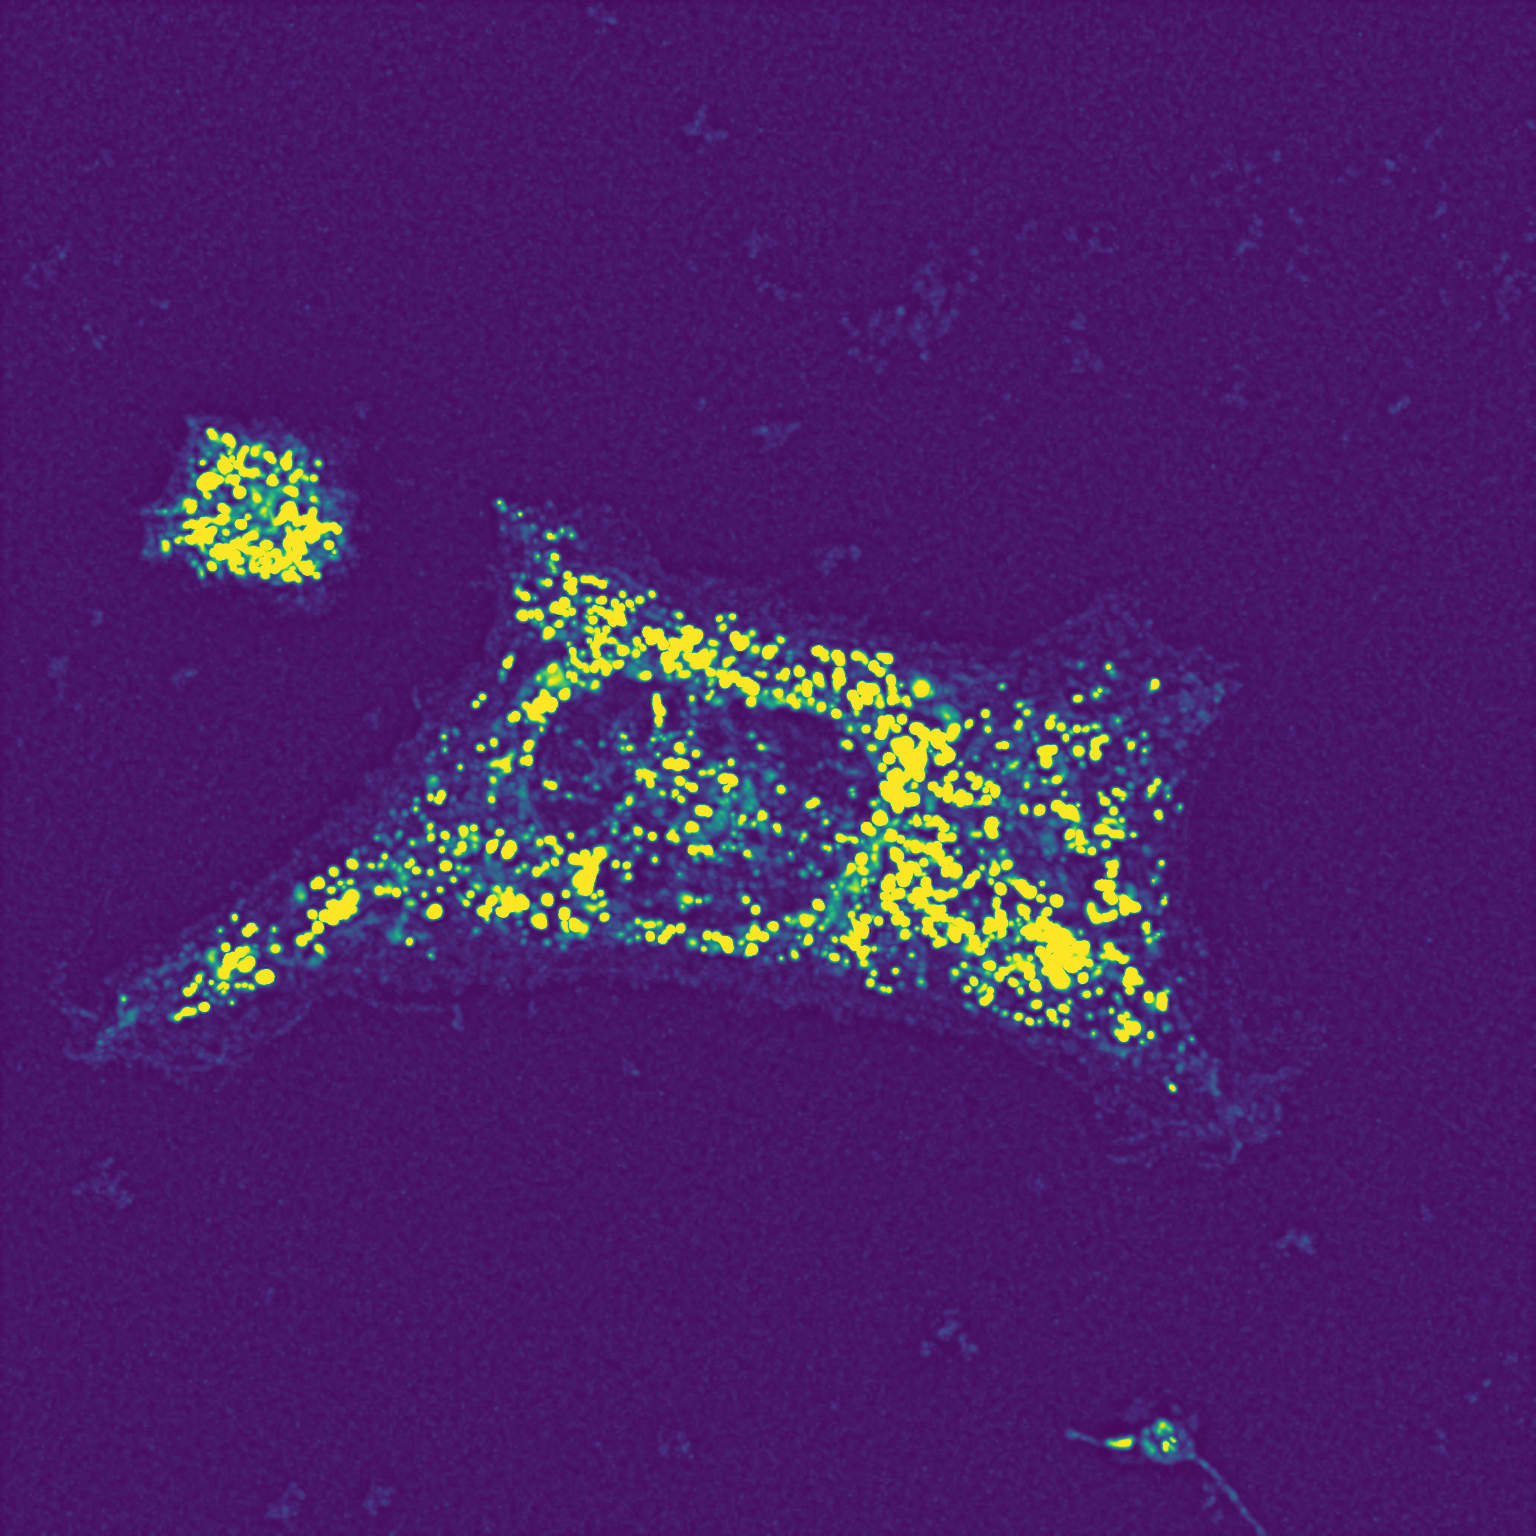
\includegraphics[width=0.3\textwidth]{figs/ch4figs/visual_analysis/raw_samples/MAX_Con_2C=0.png}}
	\subcaptionbox{Sample B intensity MIP image\label{subfig:lyso_sampl_orig_b}}{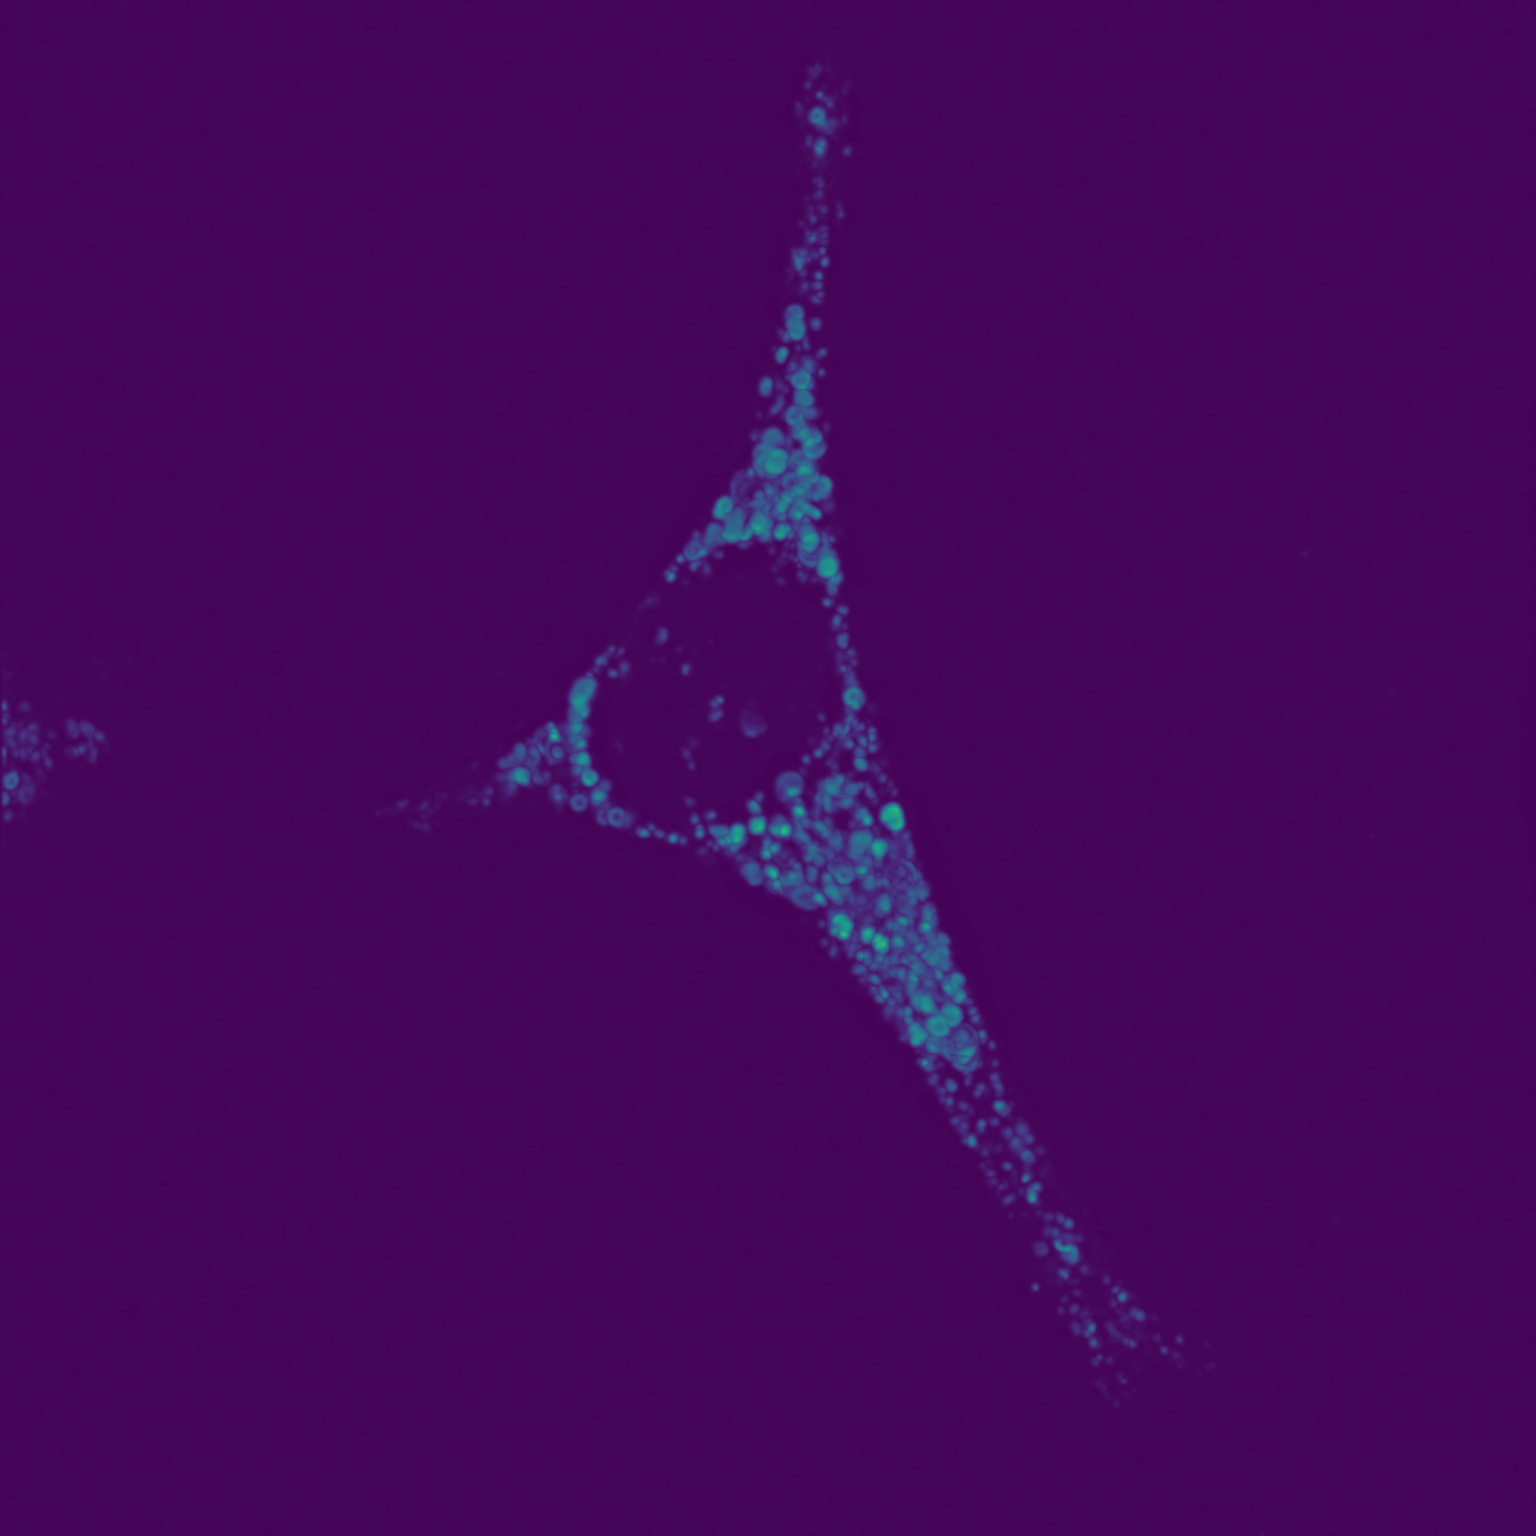
\includegraphics[width=0.3\textwidth]{figs/ch4figs/visual_analysis/raw_samples/MAX_LML_3C=0.png}}
	\subcaptionbox{Sample C intensity MIP image\label{subfig:lyso_sampl_orig_c}}{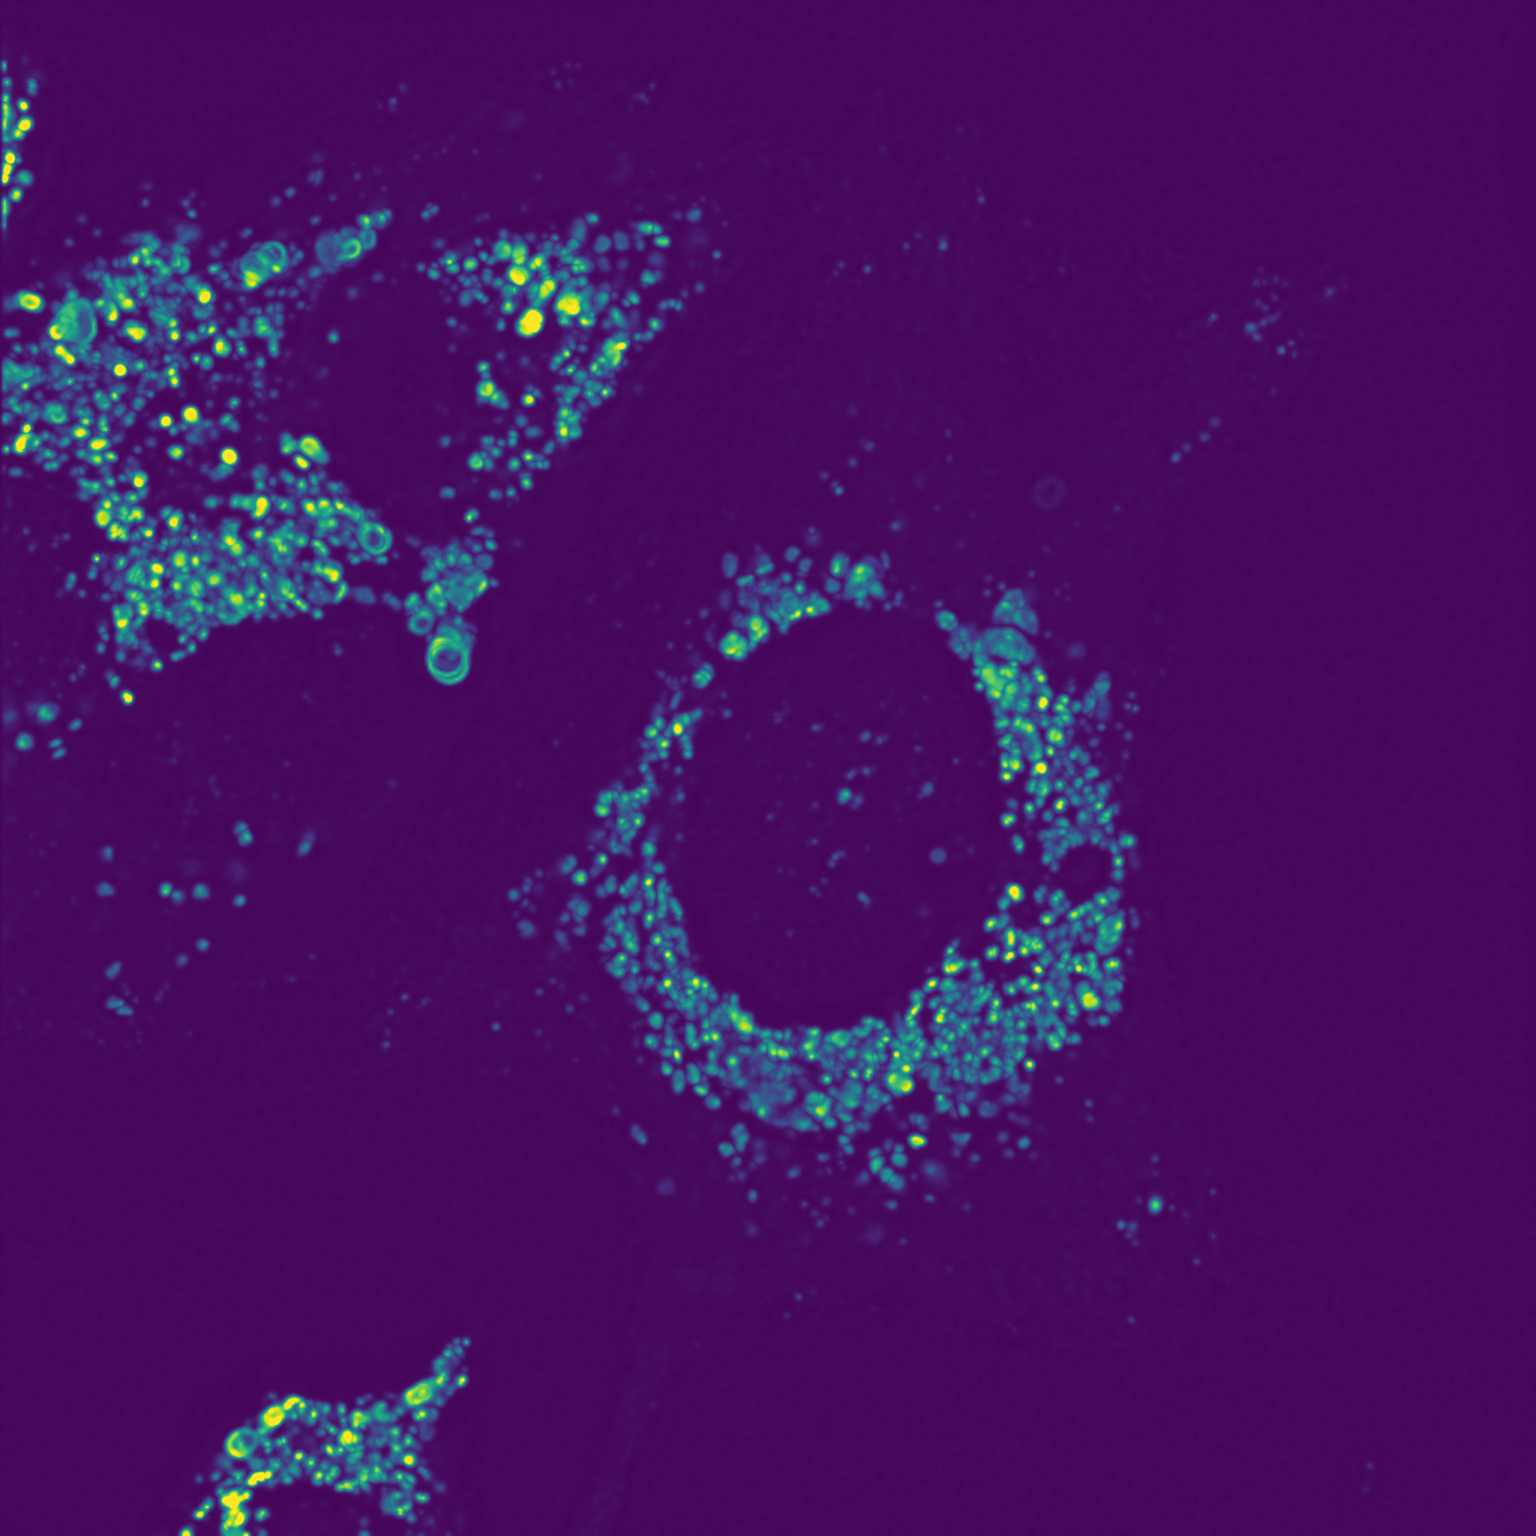
\includegraphics[width=0.3\textwidth]{figs/ch4figs/visual_analysis/raw_samples/MAX_LML_4C=0.png}}
	\subcaptionbox{Sample A centre slice\label{subfig:lyso_sampl_ec_a}}{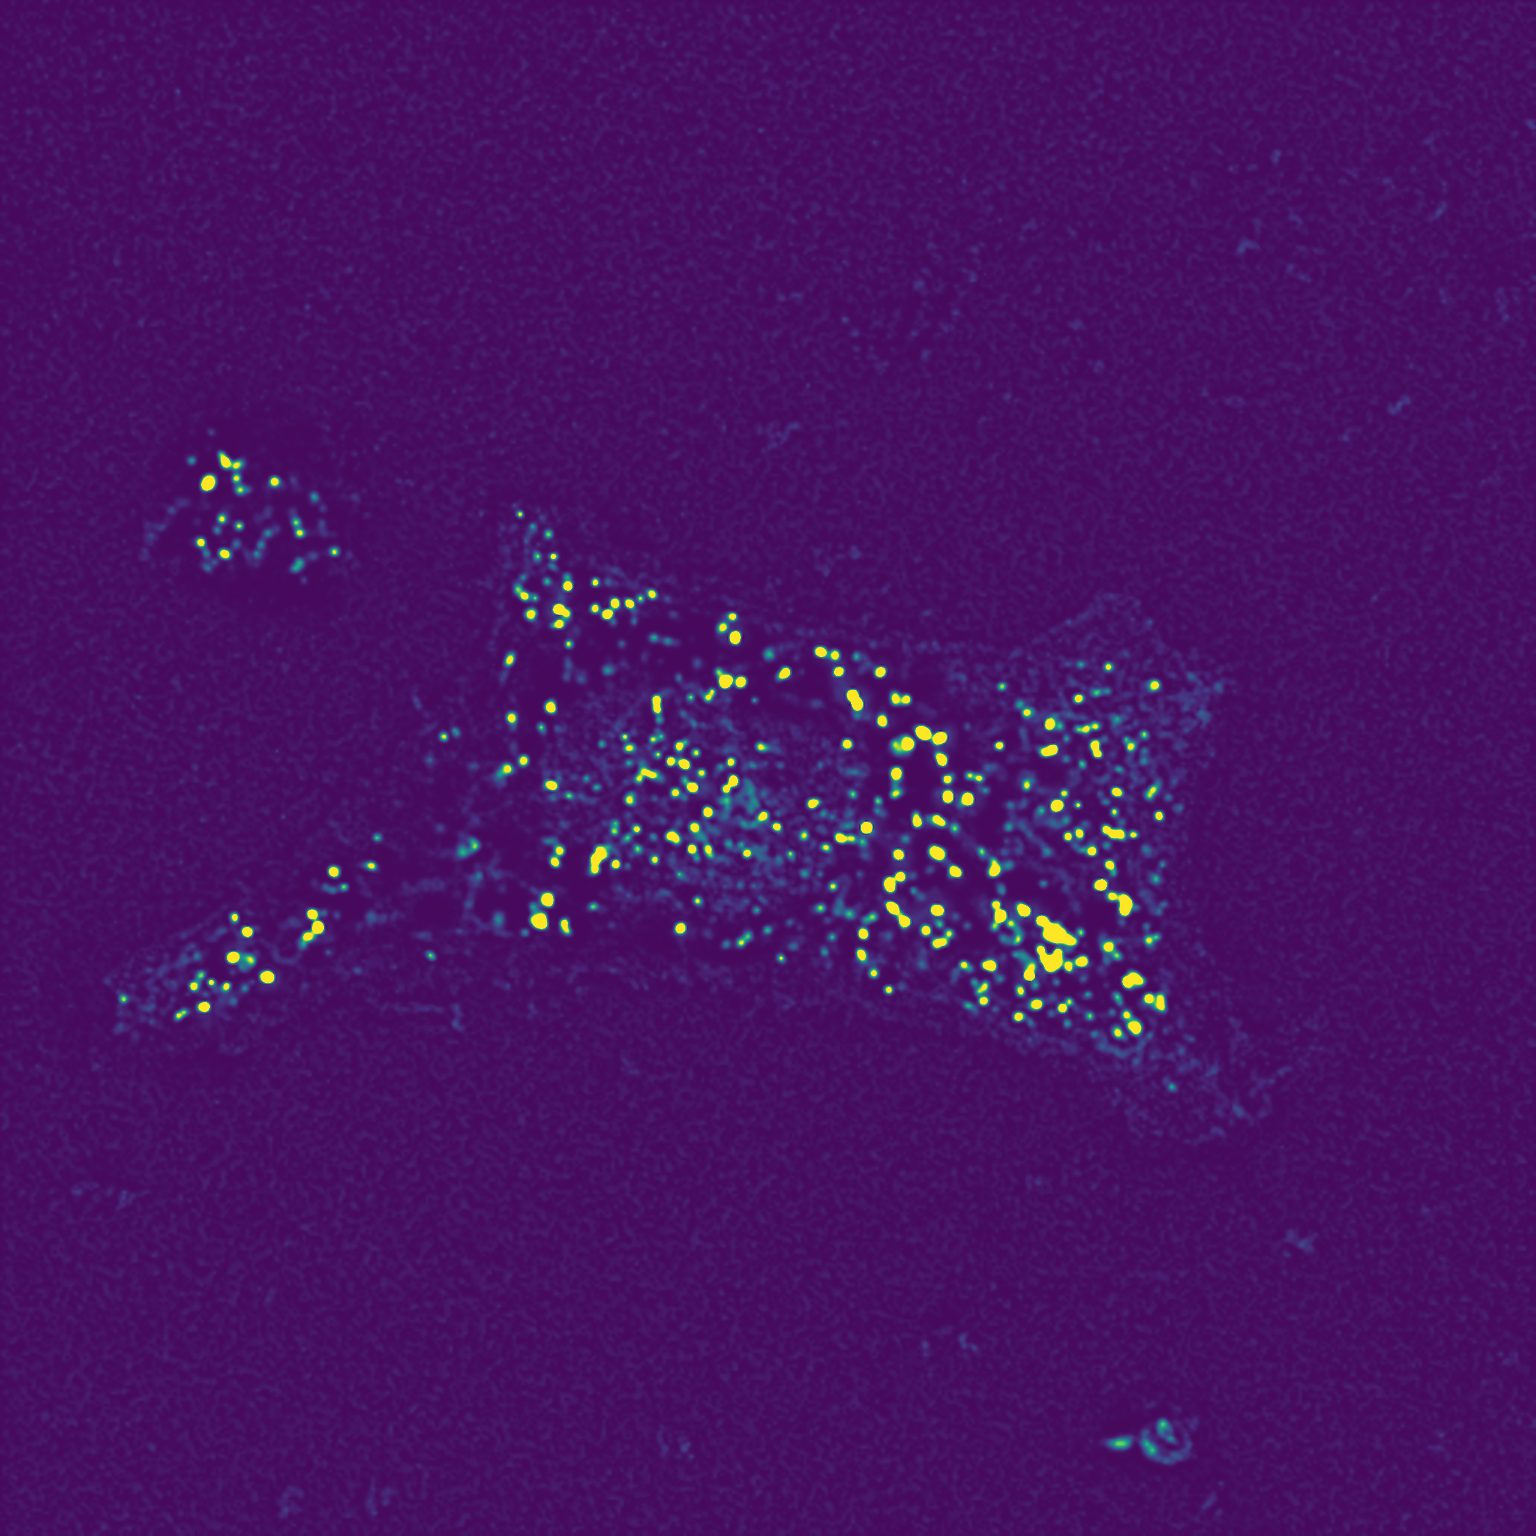
\includegraphics[width=0.3\textwidth]{figs/ch4figs/visual_analysis/raw_samples/Centre_Con_2C=0.png}}
	\subcaptionbox{Sample B centre slice\label{subfig:lyso_sampl_ec_b}}{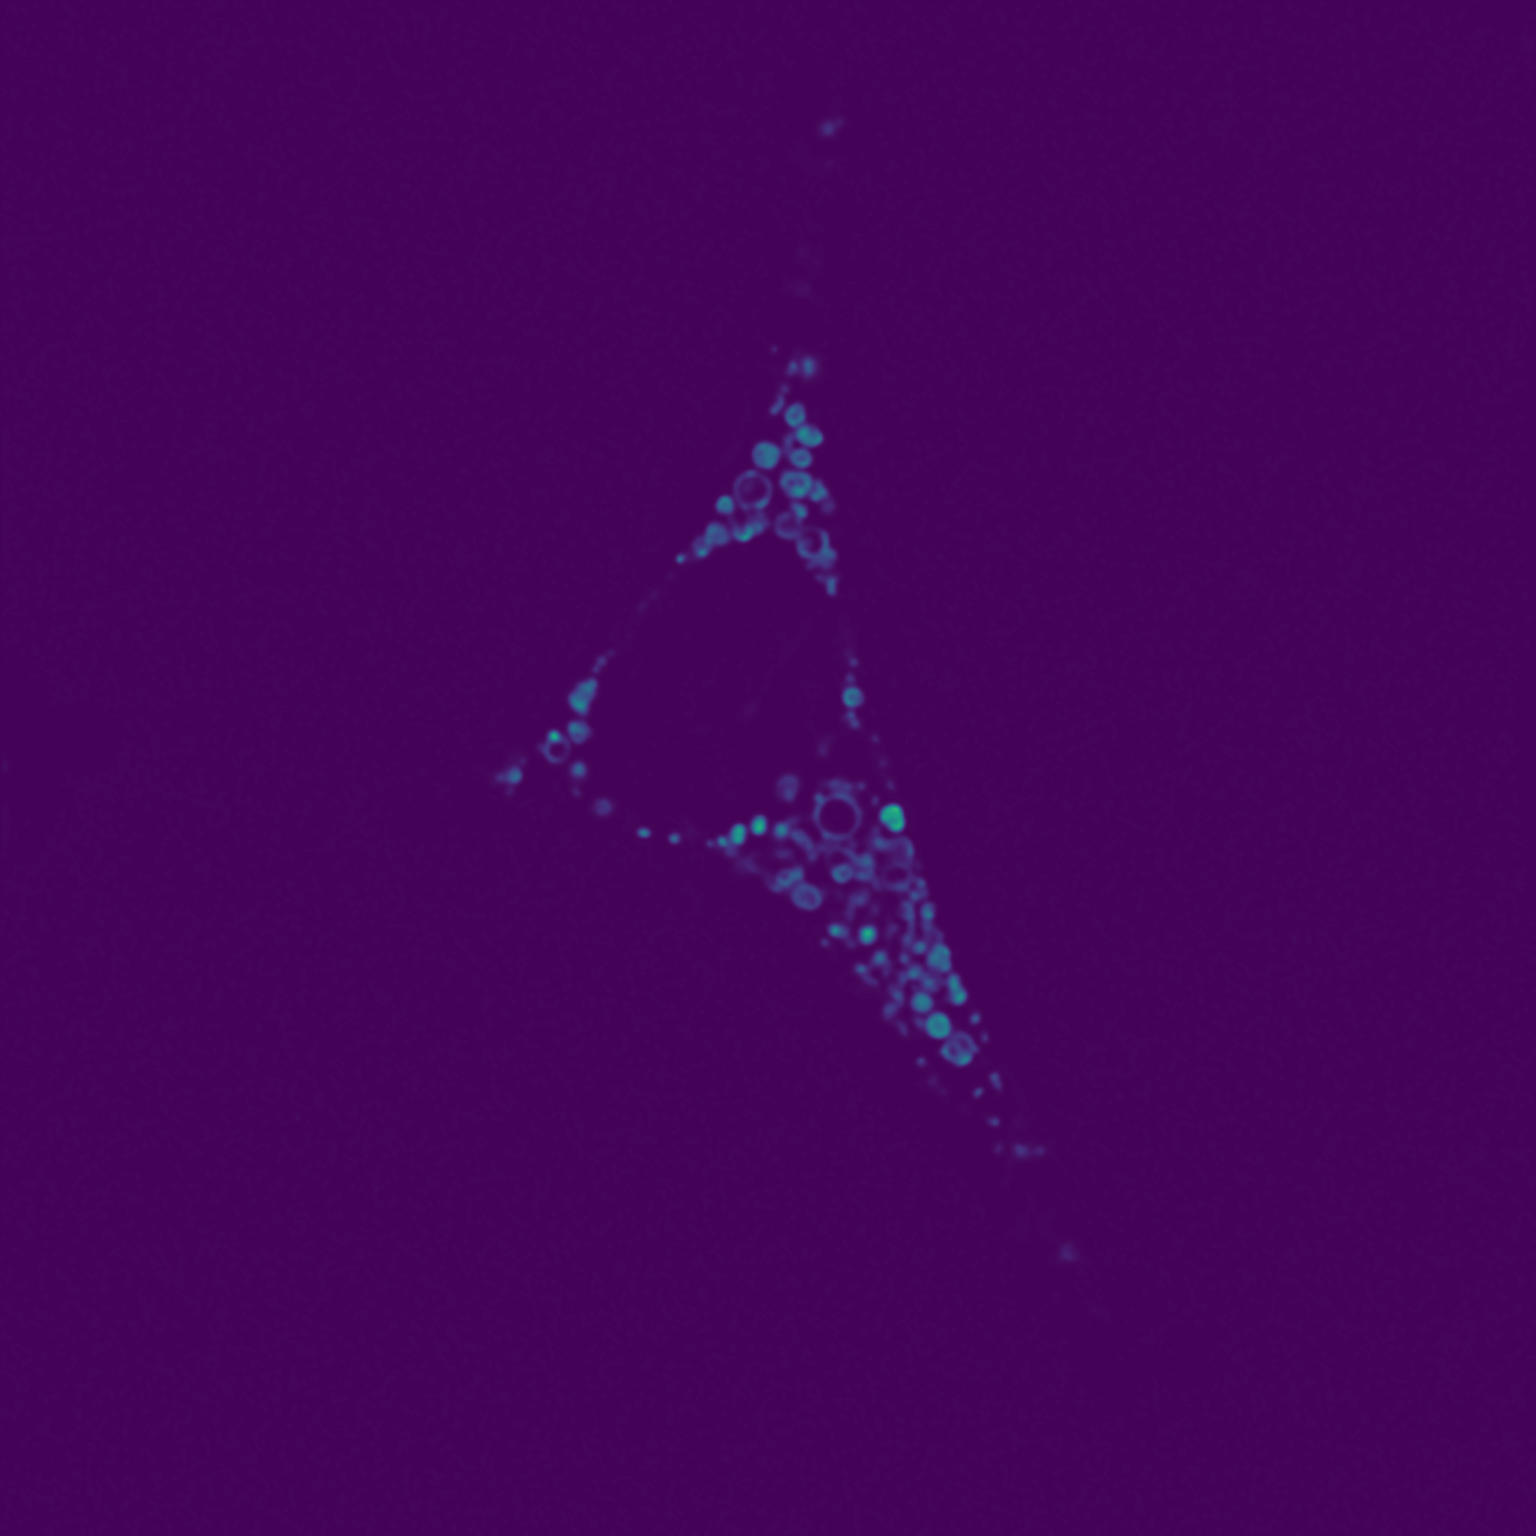
\includegraphics[width=0.3\textwidth]{figs/ch4figs/visual_analysis/raw_samples/Centre_LML_3C=0.png}}
	\subcaptionbox{Sample C centre slice\label{subfig:lyso_sampl_ec_c}}{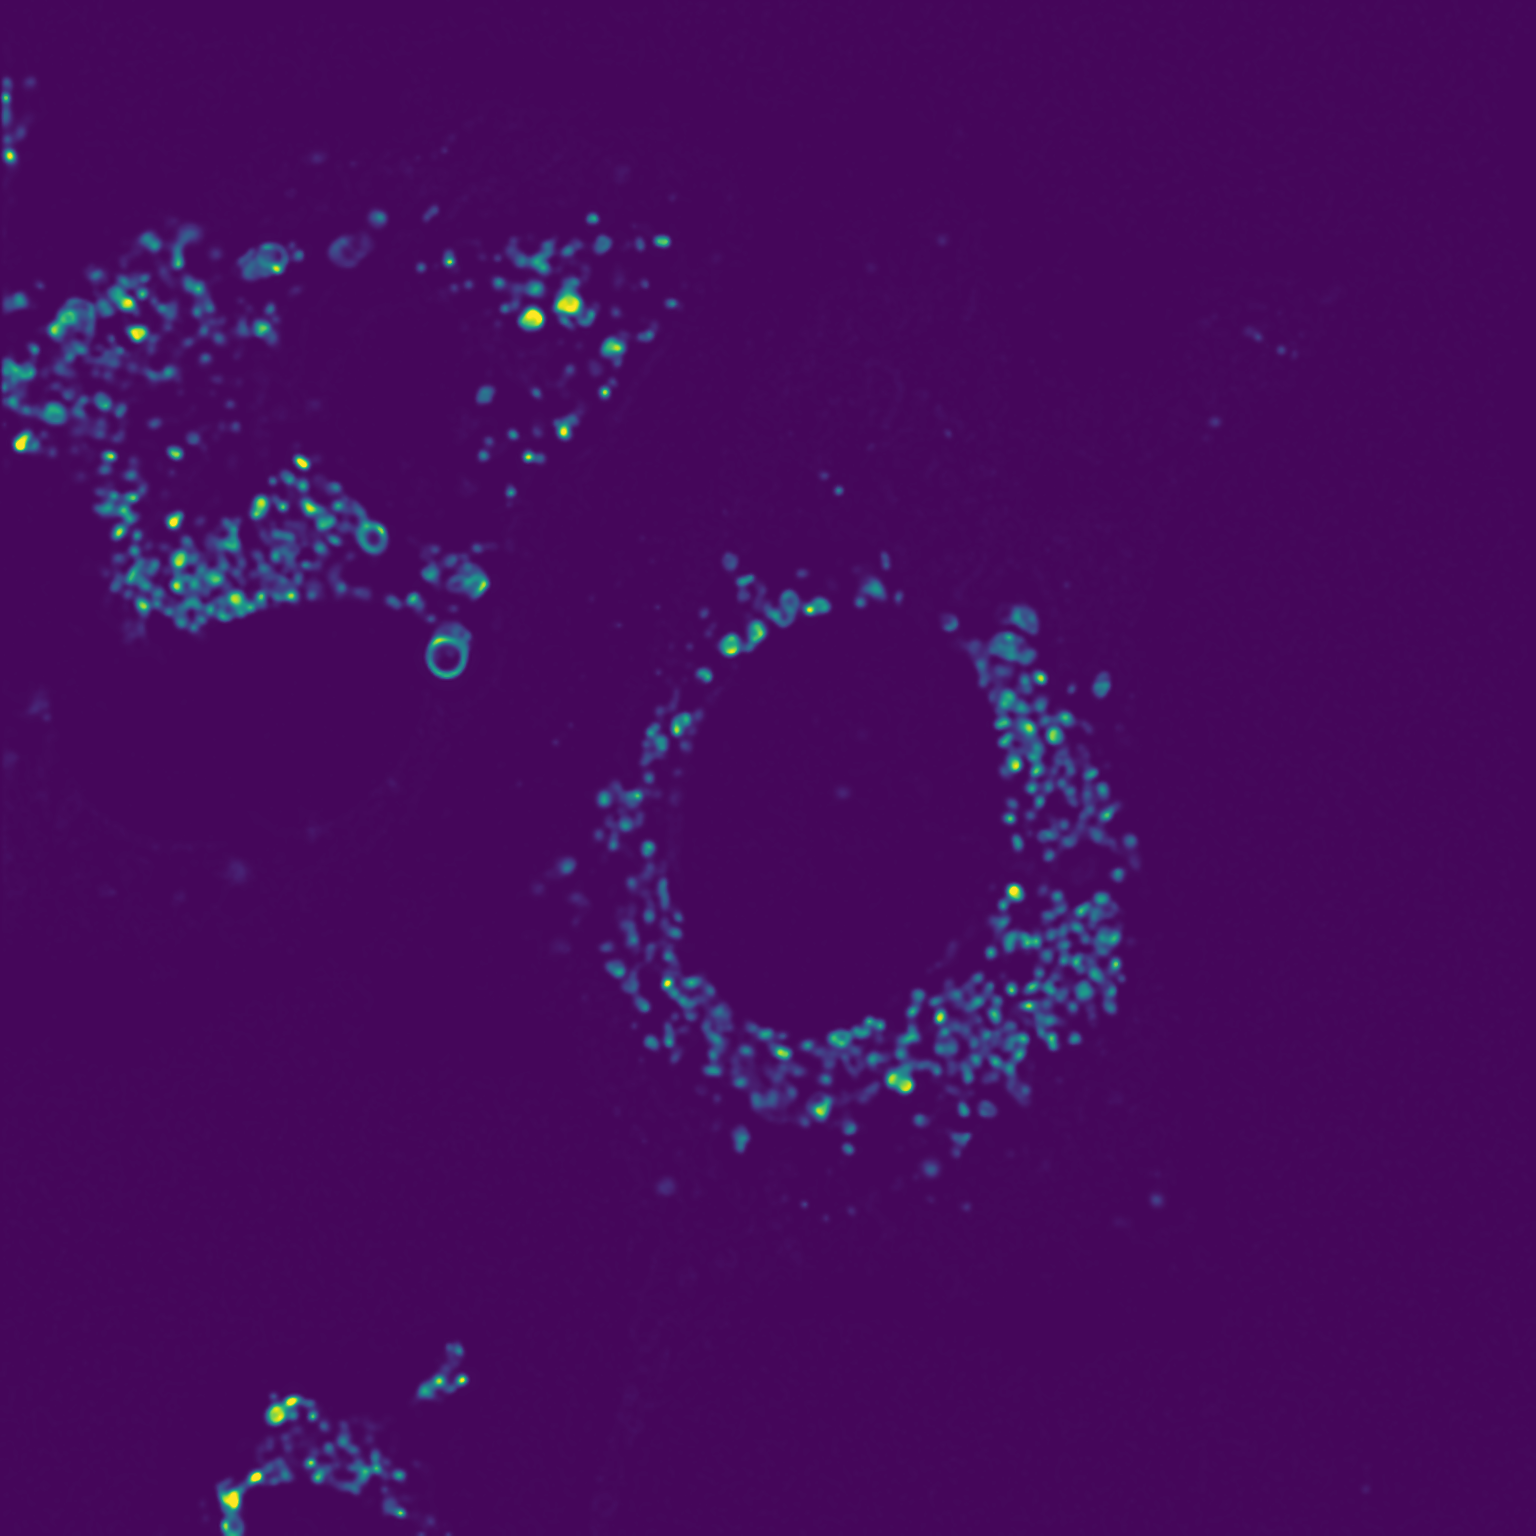
\includegraphics[width=0.3\textwidth]{figs/ch4figs/visual_analysis/raw_samples/Centre_LML_4C=0.png}}
	\caption[Image panel of the lysosome sample intensity images used in binarisation.]{Image panel for the lysosome channel of the sample images. The first row is the MIP representations and the second row is a centre slice of the intensity images prior to binarisation.}
	\label{fig:lysosome_raw}
\end{figure}
\FloatBarrier
\paragraph{Lysosome baseline:} The lysosome baseline images are presented in Figure \ref{fig:lyso_baseline} with depth projected and binarised centre slice representations in the top and bottom rows, respectively. These baseline images are produced through manually tuned Hysteresis thresholding used of the lysosome sample intensity images shown in Figure \ref{fig:lysosome_raw}. Given the previously mentioned conditions perceived for the lysosome sample intensity images, the binarisation achieved for these baselines is deemed satisfactory at worst. For sample A, the binarisation only captures the most prominent structures, based on their contrast relative to the surrounding structures and background, without any noticeable unnatural joins between them. For sample B, the structures captured in the baseline centre slice (Figure \ref{fig:lyso_baseline} \subref{subfig:lyso_centre_base}) are reflected in the respective centre slice of the sample intensity image (Figure \ref{fig:lysosome_raw} \subref{subfig:lyso_sampl_ec_b}) with the brightest structures being captured in the foreground while excluding a number of the dim out-of-focus structures seen. For sample C, it is believed that the brightest structures have been captured without excessive fragmentation, but there may be a few cases of falsely joined structures. Due to the conditions of this sample, as mentioned previously, this was not unexpected, and the degree of joining presented is not to a concerning degree, especially since false joining could be remedied with further image processing while fragmentation cannot be restored. Overall, it is believed that the baseline binarisation achieved is adequate for any succeeding analysis, with only samples B and C providing some minor uncertainty but not to the extent it will jeopardise any analysis.

\begin{figure}[ht!]
	\centering
	\subcaptionbox{Sample A}{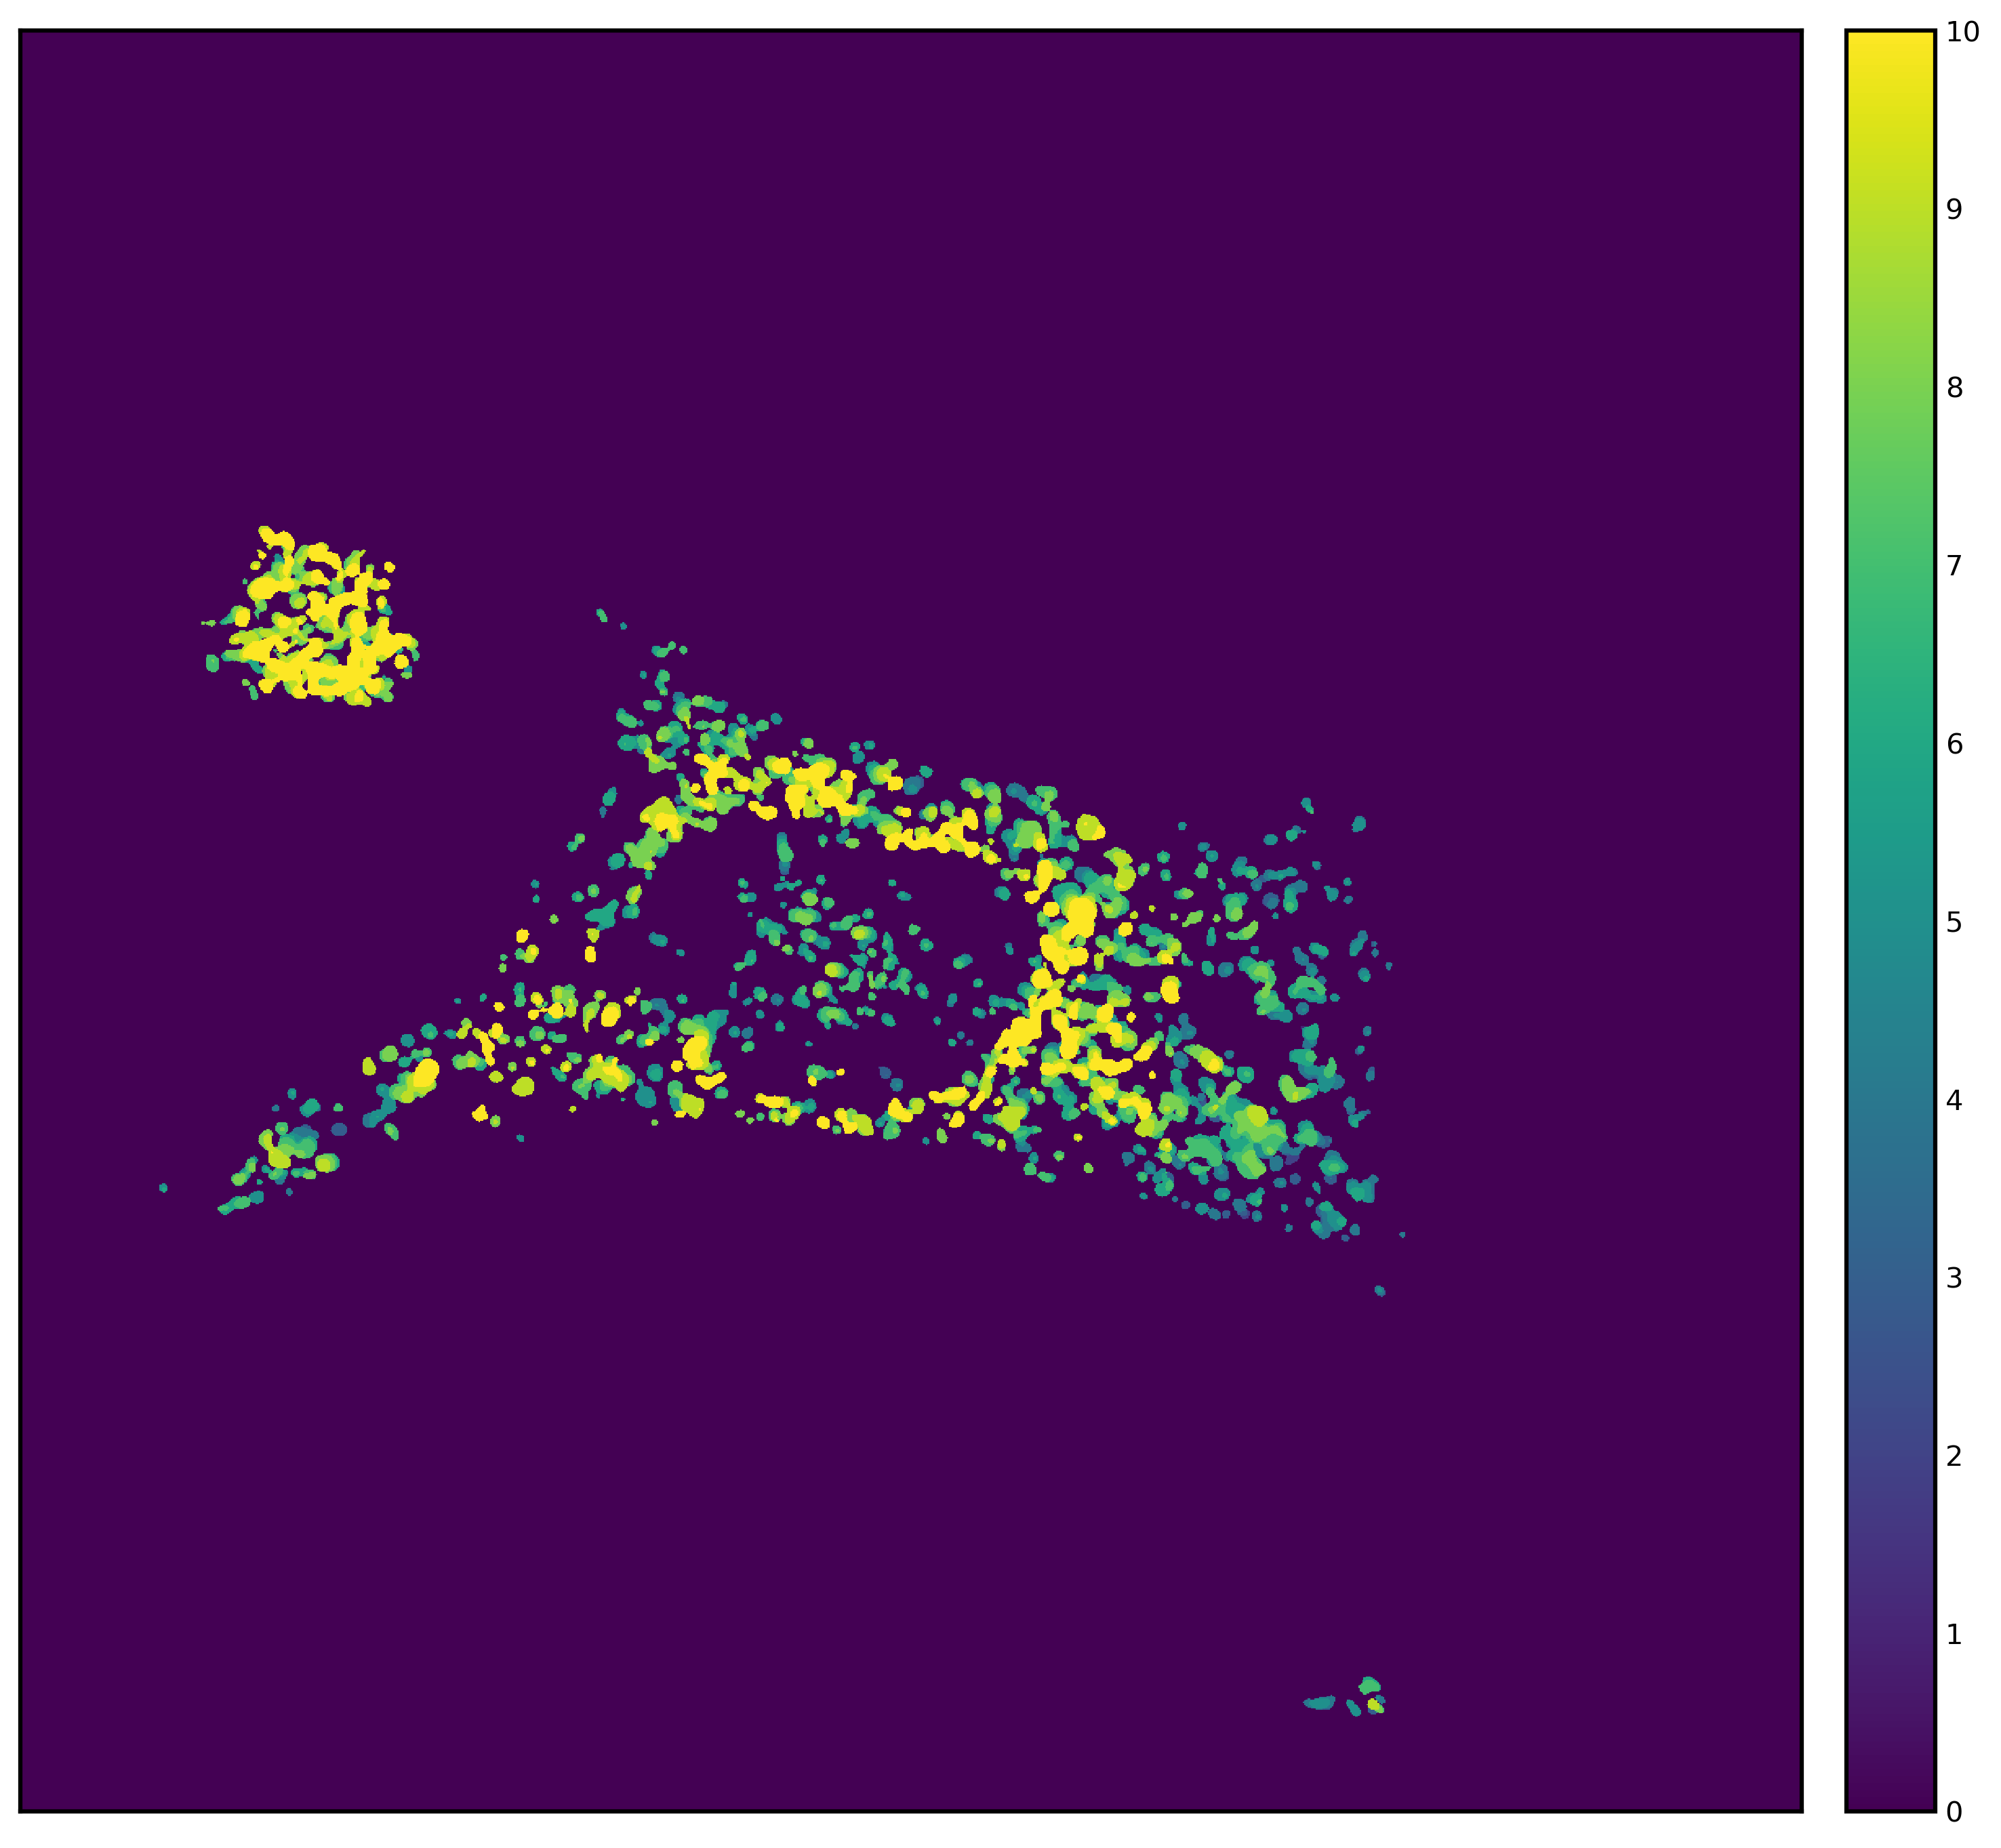
\includegraphics[width=0.28\textwidth]{figs/ch4figs/visual_analysis/raw_samples/Flat_Con_2C=0_Hyst.png}}
	\subcaptionbox{Sample B}{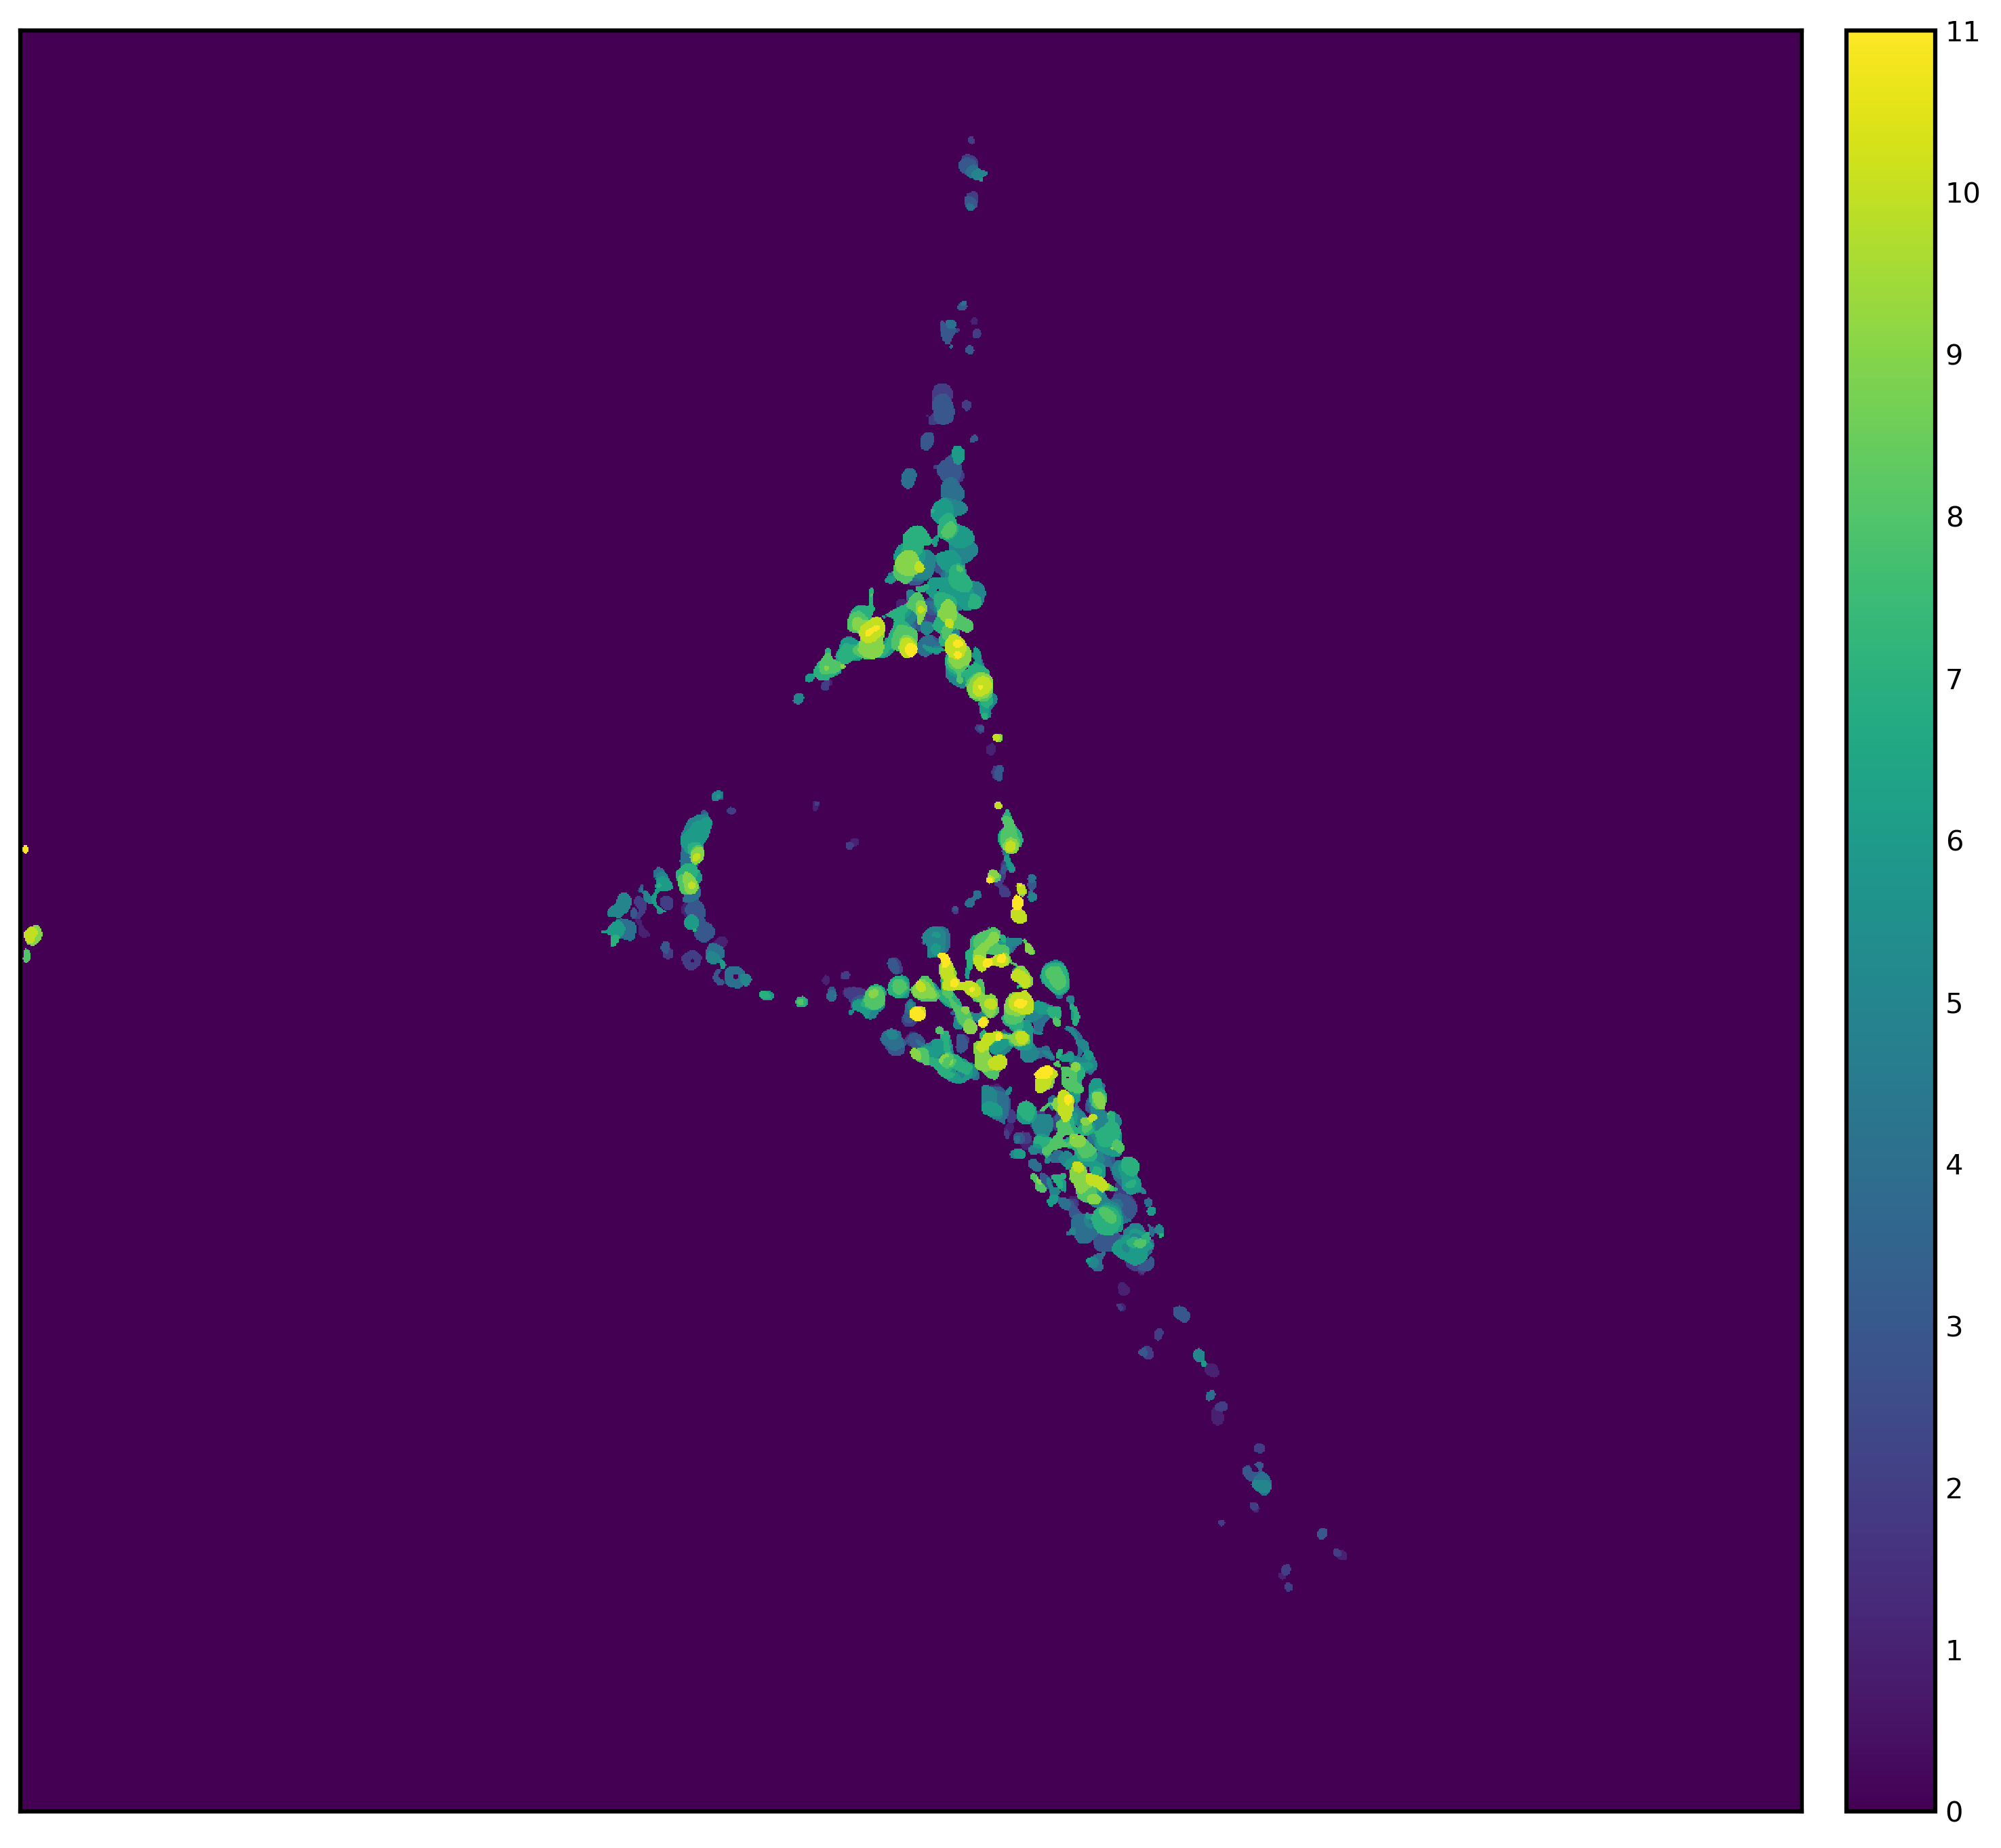
\includegraphics[width=0.28\textwidth]{figs/ch4figs/visual_analysis/raw_samples/Flat_LML_3C=0_Hyst.png}}
	\subcaptionbox{Sample C}{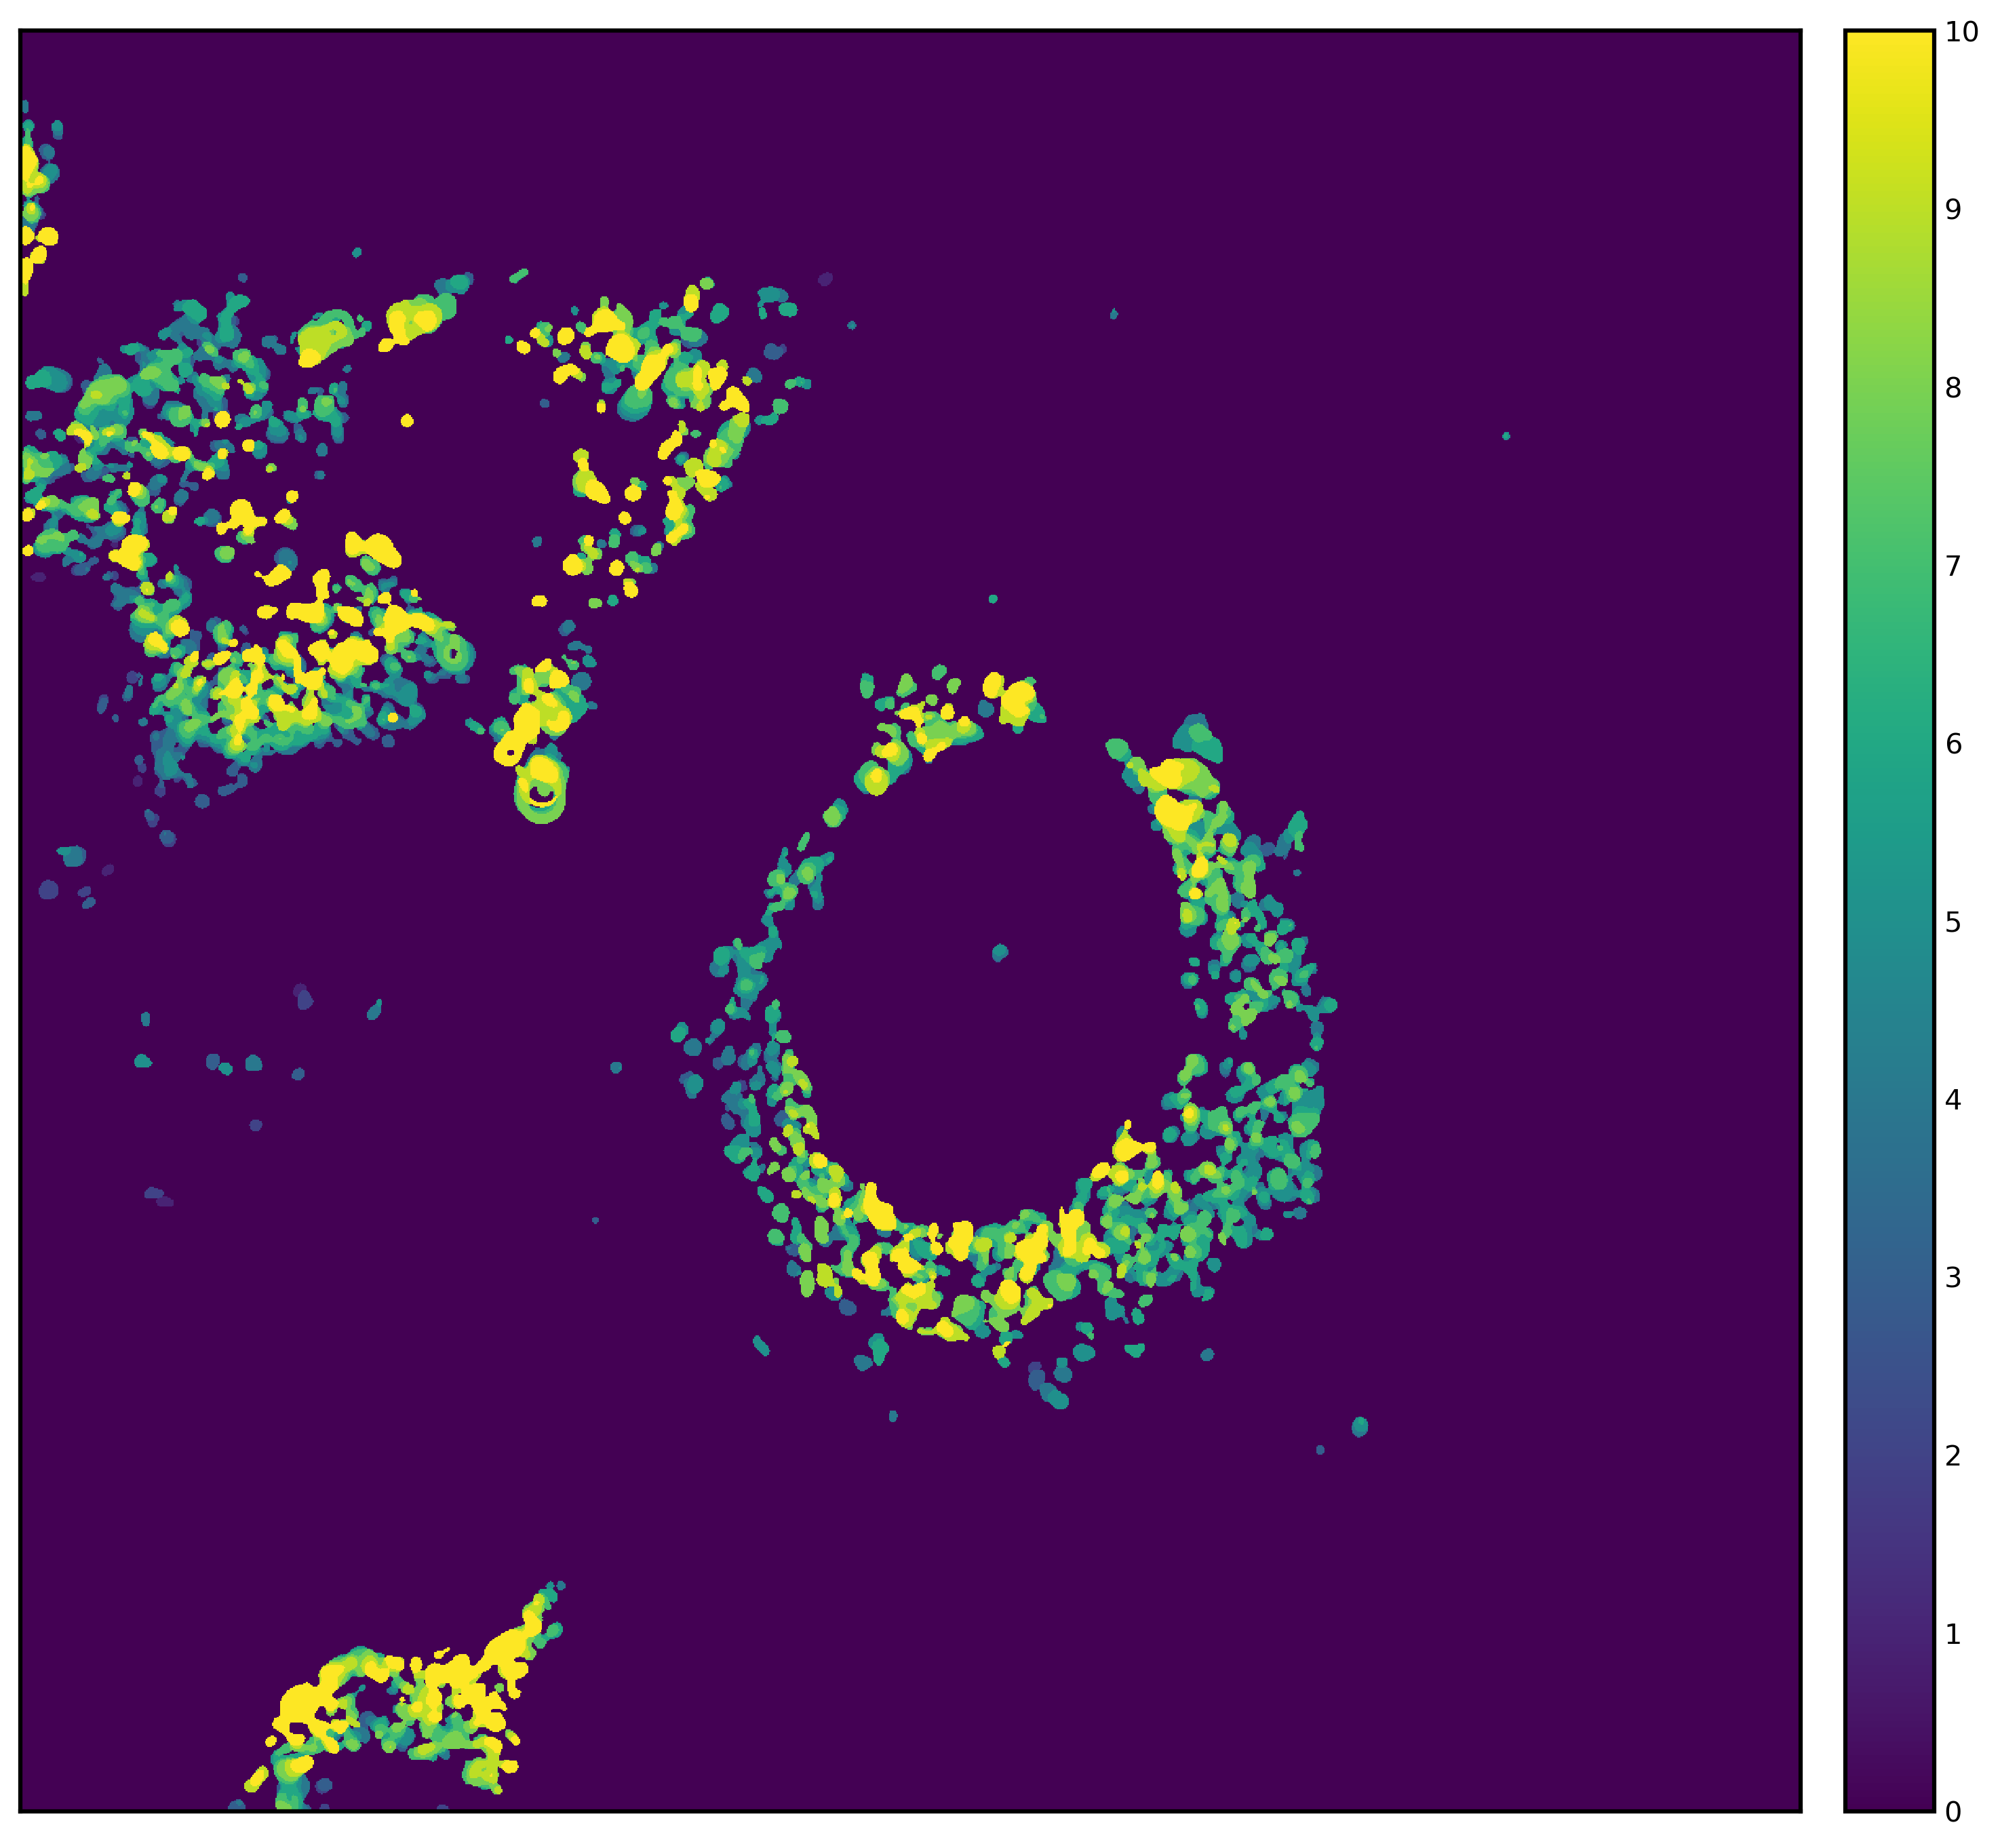
\includegraphics[width=0.28\textwidth]{figs/ch4figs/visual_analysis/raw_samples/Flat_LML_4C=0_Hyst.png}}
	\subcaptionbox{Sample A centre slice}{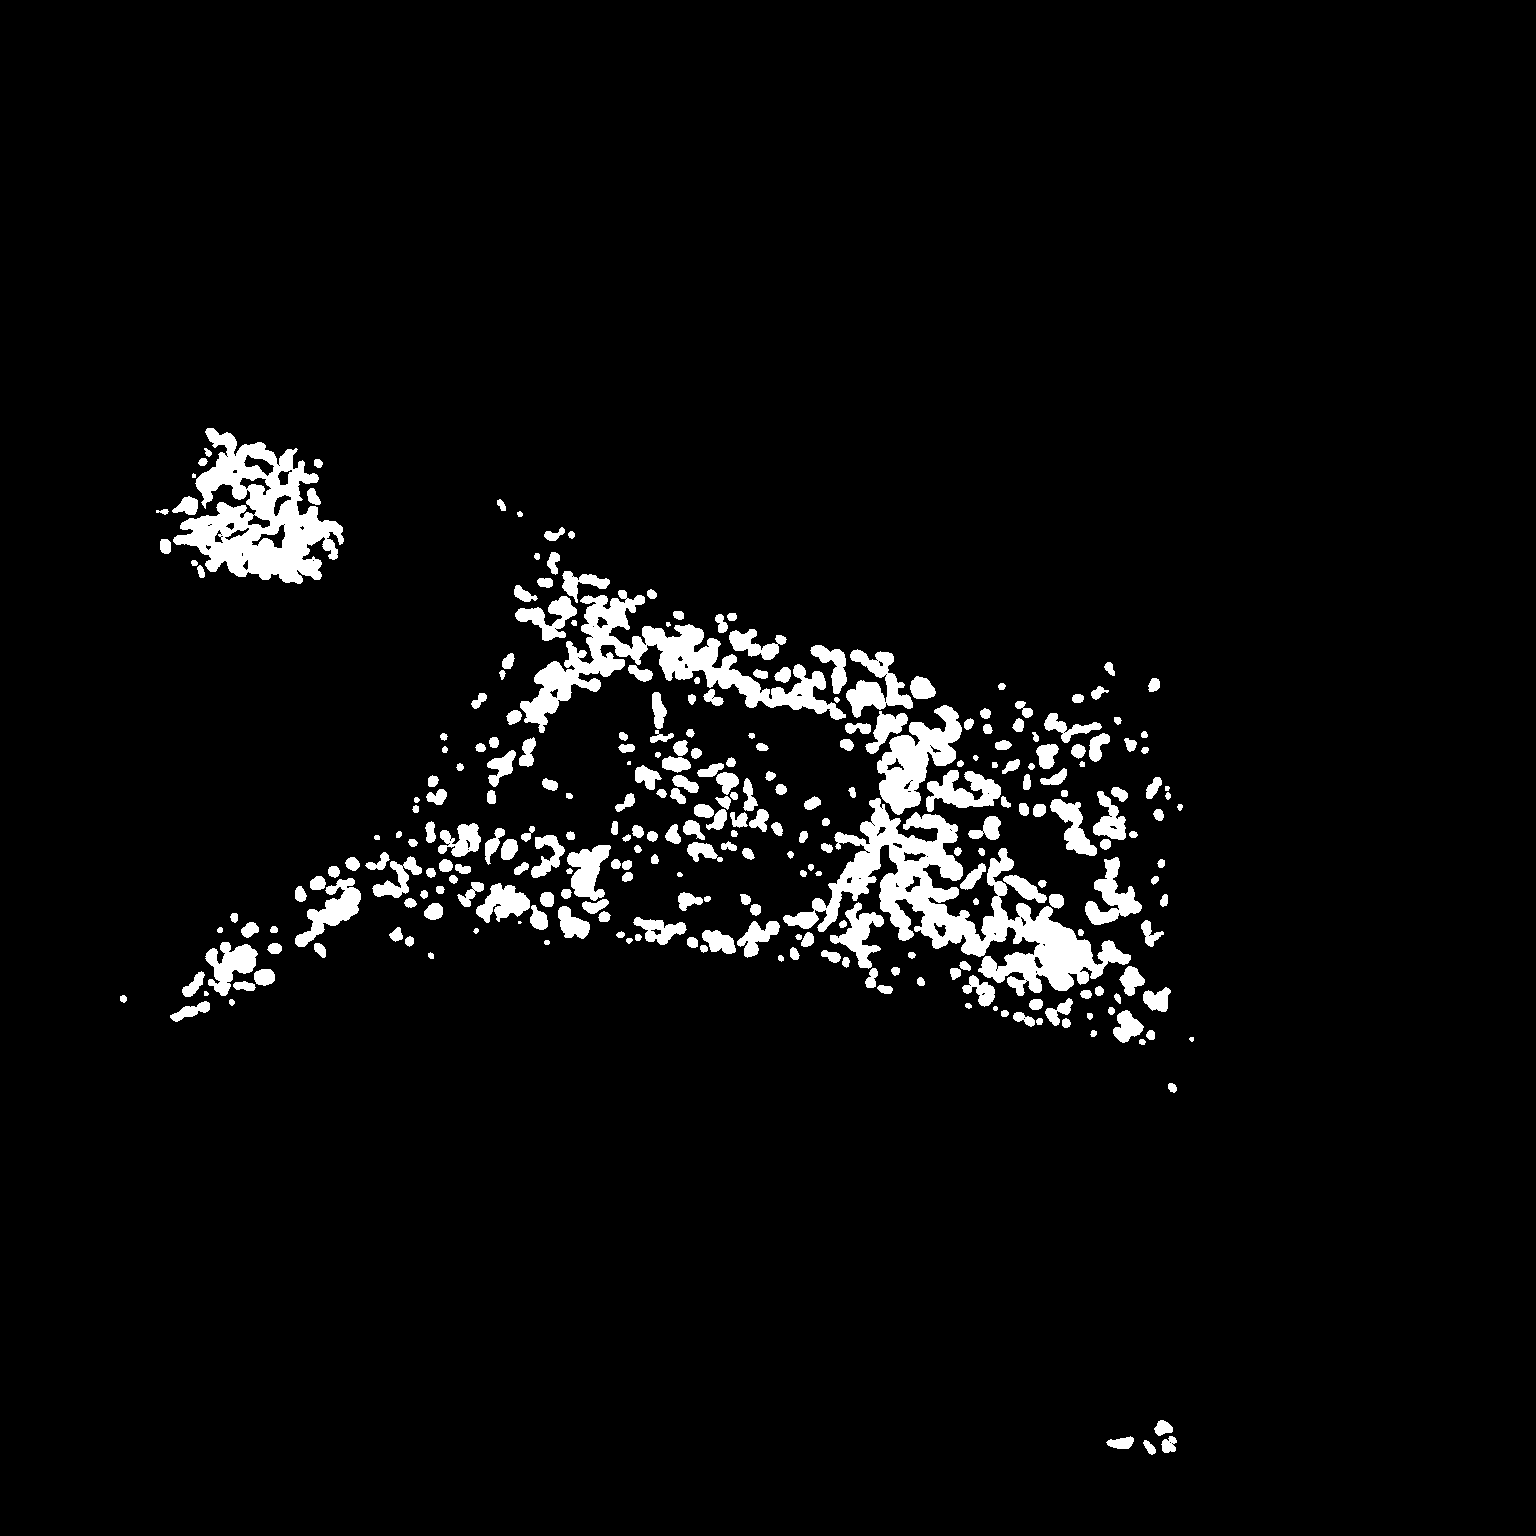
\includegraphics[width=0.28\textwidth]{figs/ch4figs/visual_analysis/raw_samples/Hyst_Con_2C=0.png}}
	\subcaptionbox{Sample B centre slice\label{subfig:lyso_centre_base}}{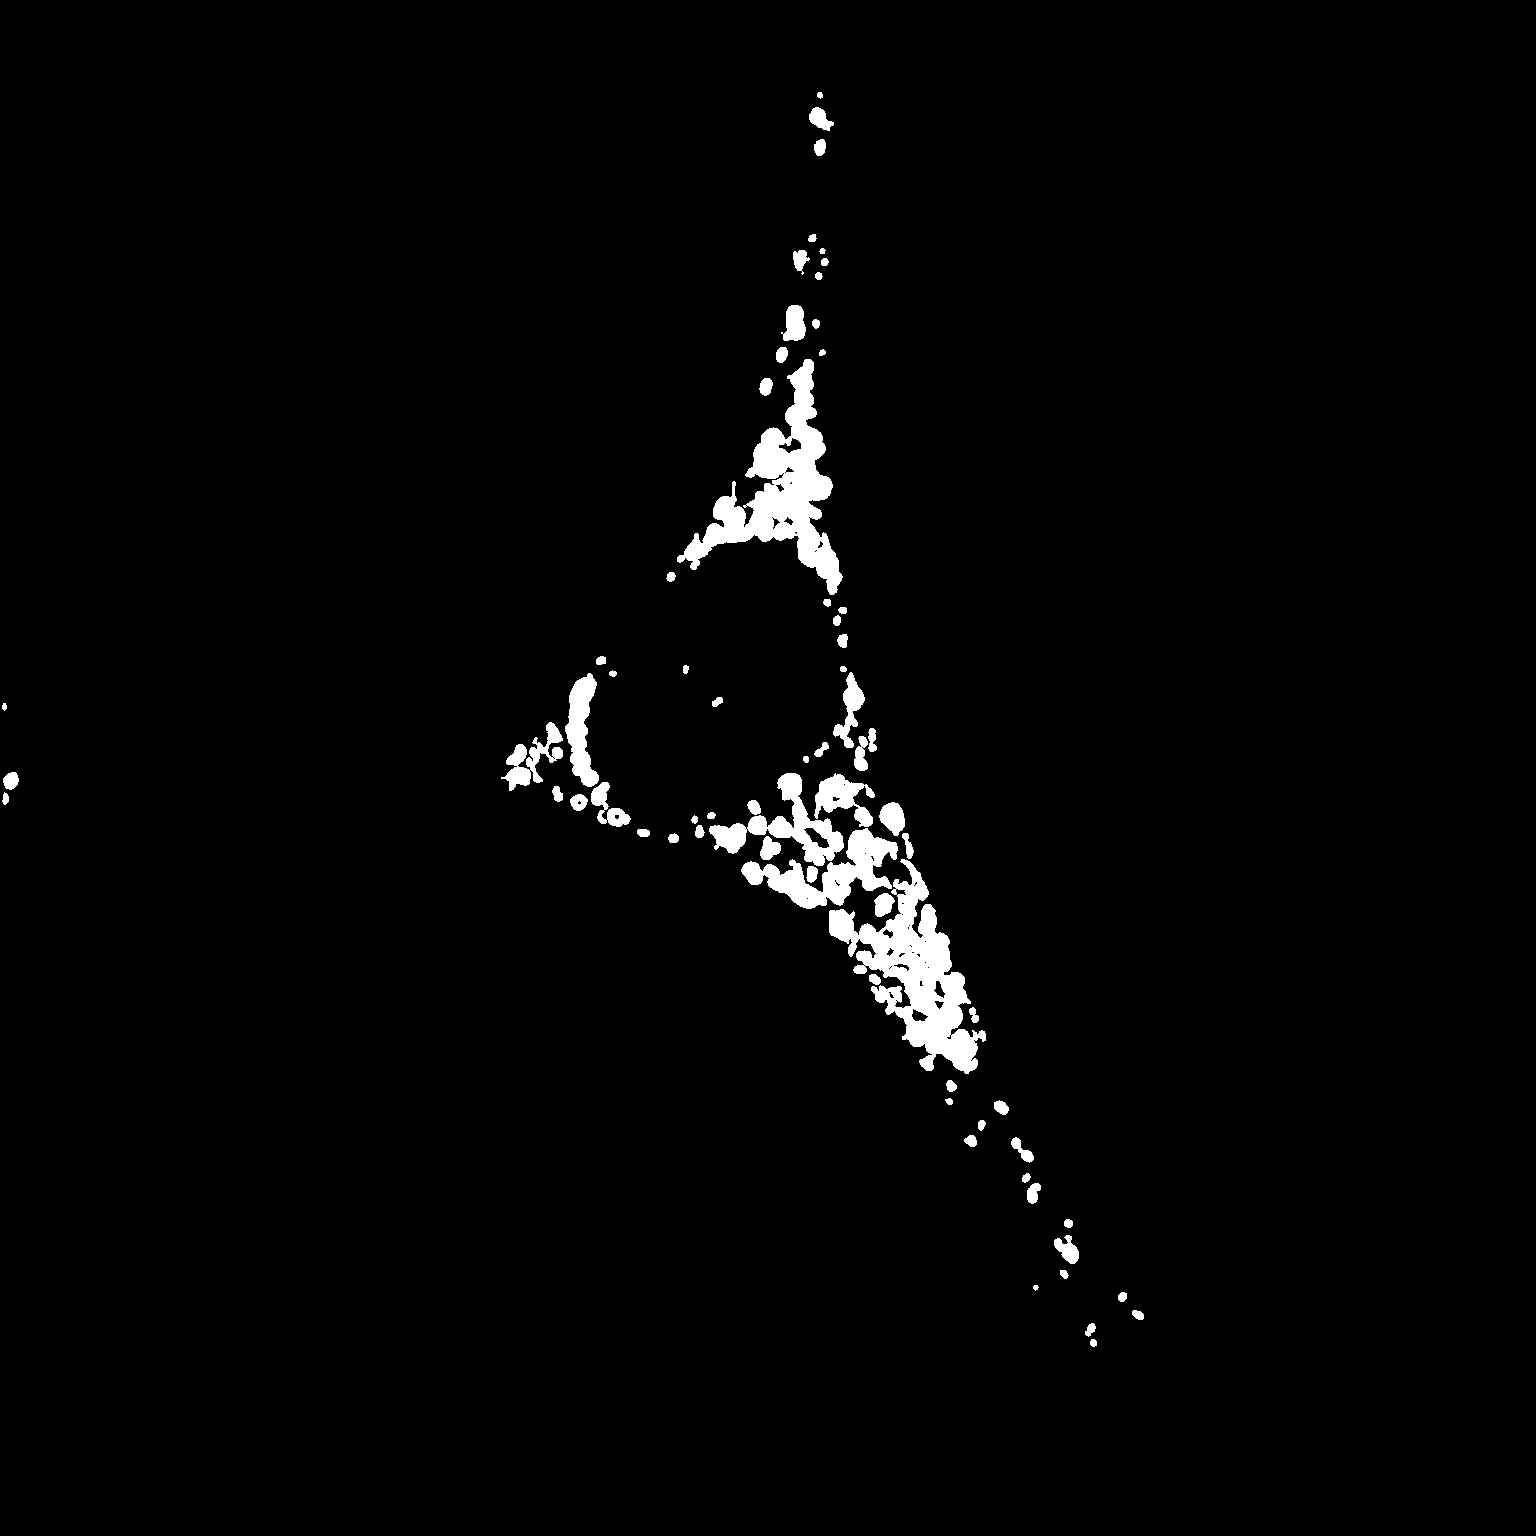
\includegraphics[width=0.28\textwidth]{figs/ch4figs/visual_analysis/raw_samples/Hyst_LML_3C=0.png}}
	\subcaptionbox{Sample C centre slice}{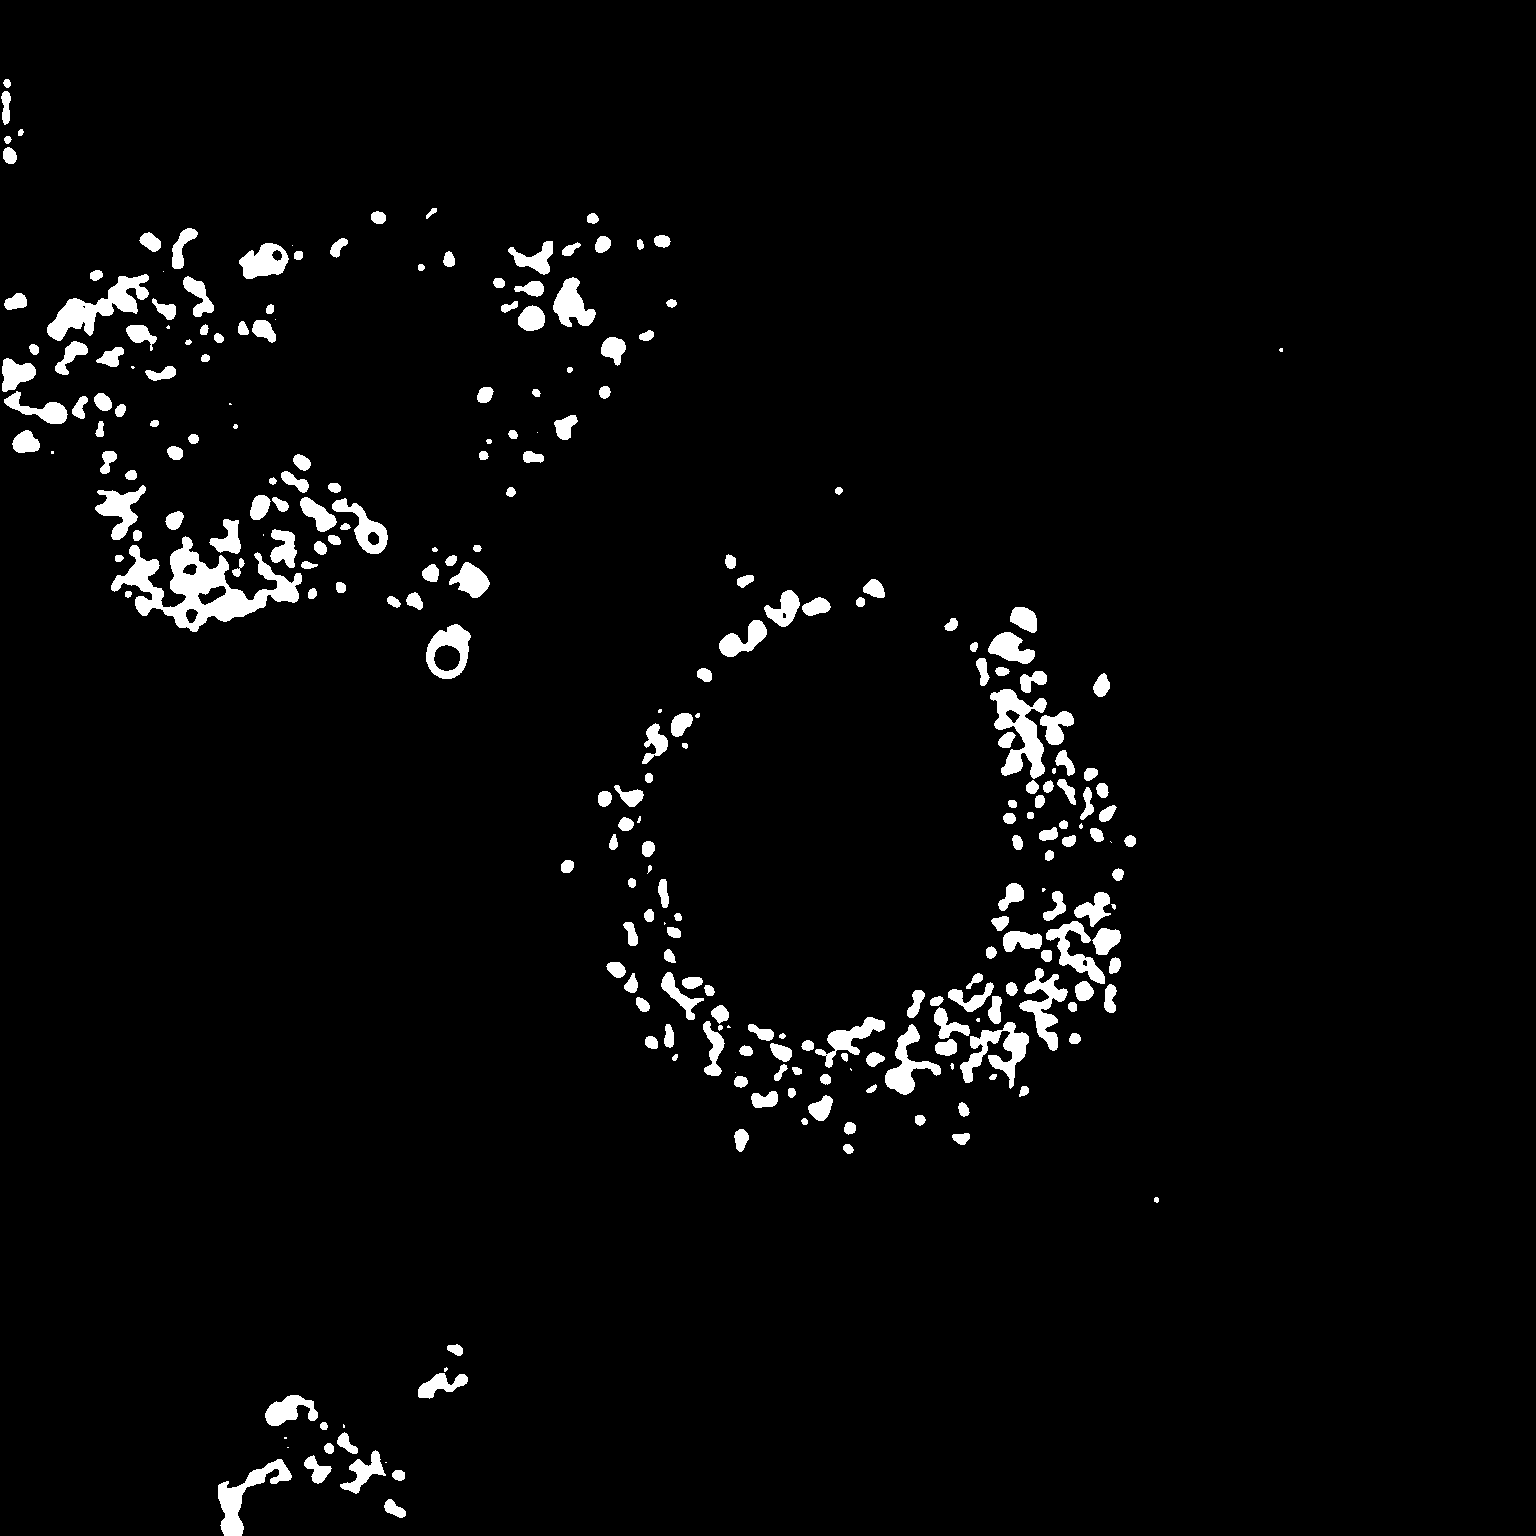
\includegraphics[width=0.28\textwidth]{figs/ch4figs/visual_analysis/raw_samples/Hyst_LML_4C=0.png}}
	\caption[Showcase of the baseline binarisations for each lysosome sample image.]{Showcase of the baseline binarisations for each lysosome sample image, generated through manually tuned Hysteresis thresholding, and depicted using both depth projection and binary centre slice images with the former in the top row and the latter in the bottom row. The respective lysosome sample intensity images used are shown in Figure \ref{fig:lysosome_raw}.}
	\label{fig:lyso_baseline}
\end{figure}

\subsubsection{Global thresholding methods}
For the lysosome structures the top two global thresholding methods are IsoData and Otsu based on the total scores in Table \ref{tab:lyso_global_ranks}.
\begin{table}[hb!]
	\centering
	\begin{tabular}{|c|c|c|c|c|}
		\hline
		\textbf{Method} & \textbf{Sample A} & \textbf{Sample B} & \textbf{Sample C} & \textbf{Mean score}\\
		\hline
		Otsu & 5 & 4 & 5 & 4.6 \\
		\hline
		IsoData & 5 & 4 & 5 & 4.6 \\
		\hline
		\textit{Baseline} & 5 & 4 & 4 & 4.3\\
		\hline
		Moments & 4 & 4 & 4 & 4 \\
		\hline
		MaxEntropy & 2 & 4 & 3 & 3 \\
		\hline
		RenyiEntropy & 1 & 4 & 3 & 2.6 \\
		\hline
		Yen & 1 & 4 & 3 & 2.6 \\
		\hline
		Huang2 & 1 & 3 & 2 & 2 \\
		\hline
		Li & 2 & 2 & 2 & 2 \\
		\hline
		Triangle & 1 & 2 & 1 & 1.3 \\
		\hline
		
	\end{tabular}
	\caption[A score for each method's binarisation of the lysosome sample images with an overall mean score provided.]{A score for each method's binarisation of the lysosome sample images with an overall mean score provided. The methods are ranked in descending order based on their mean score.}
	\label{tab:lyso_global_ranks}
\end{table}
%Note for sample B that methods such as Huang2 and Li express excessive joining but the intensity range of the image is abnormally low
\FloatBarrier
\paragraph{IsoData} The IsoData binarisations of the lysosome sample images are showcased in Figure \ref{fig:lyso_isodata}, which are represented by both depth projections and a red-green (RG) overlay of the IsoData and baseline binarisations for each sample's centre slice. The results across all images are similar for the IsoData and the baseline, observed in Figure \ref{fig:lyso_isodata} (\subref{subfig:lyso_rg_isodata_a}-\subref{subfig:lyso_rg_isodata_c}), with the primary difference being a small increase in foreground structures for all lysosome samples. Sample-specific differences, against the baseline, are that the volumes of structures are slightly increased for sample B, and there is a decrease in joined structures but not to the extent that it would be perceived as structure fragmentation.

\begin{figure}[h!]
	\centering
	\subcaptionbox{Sample A depth project}{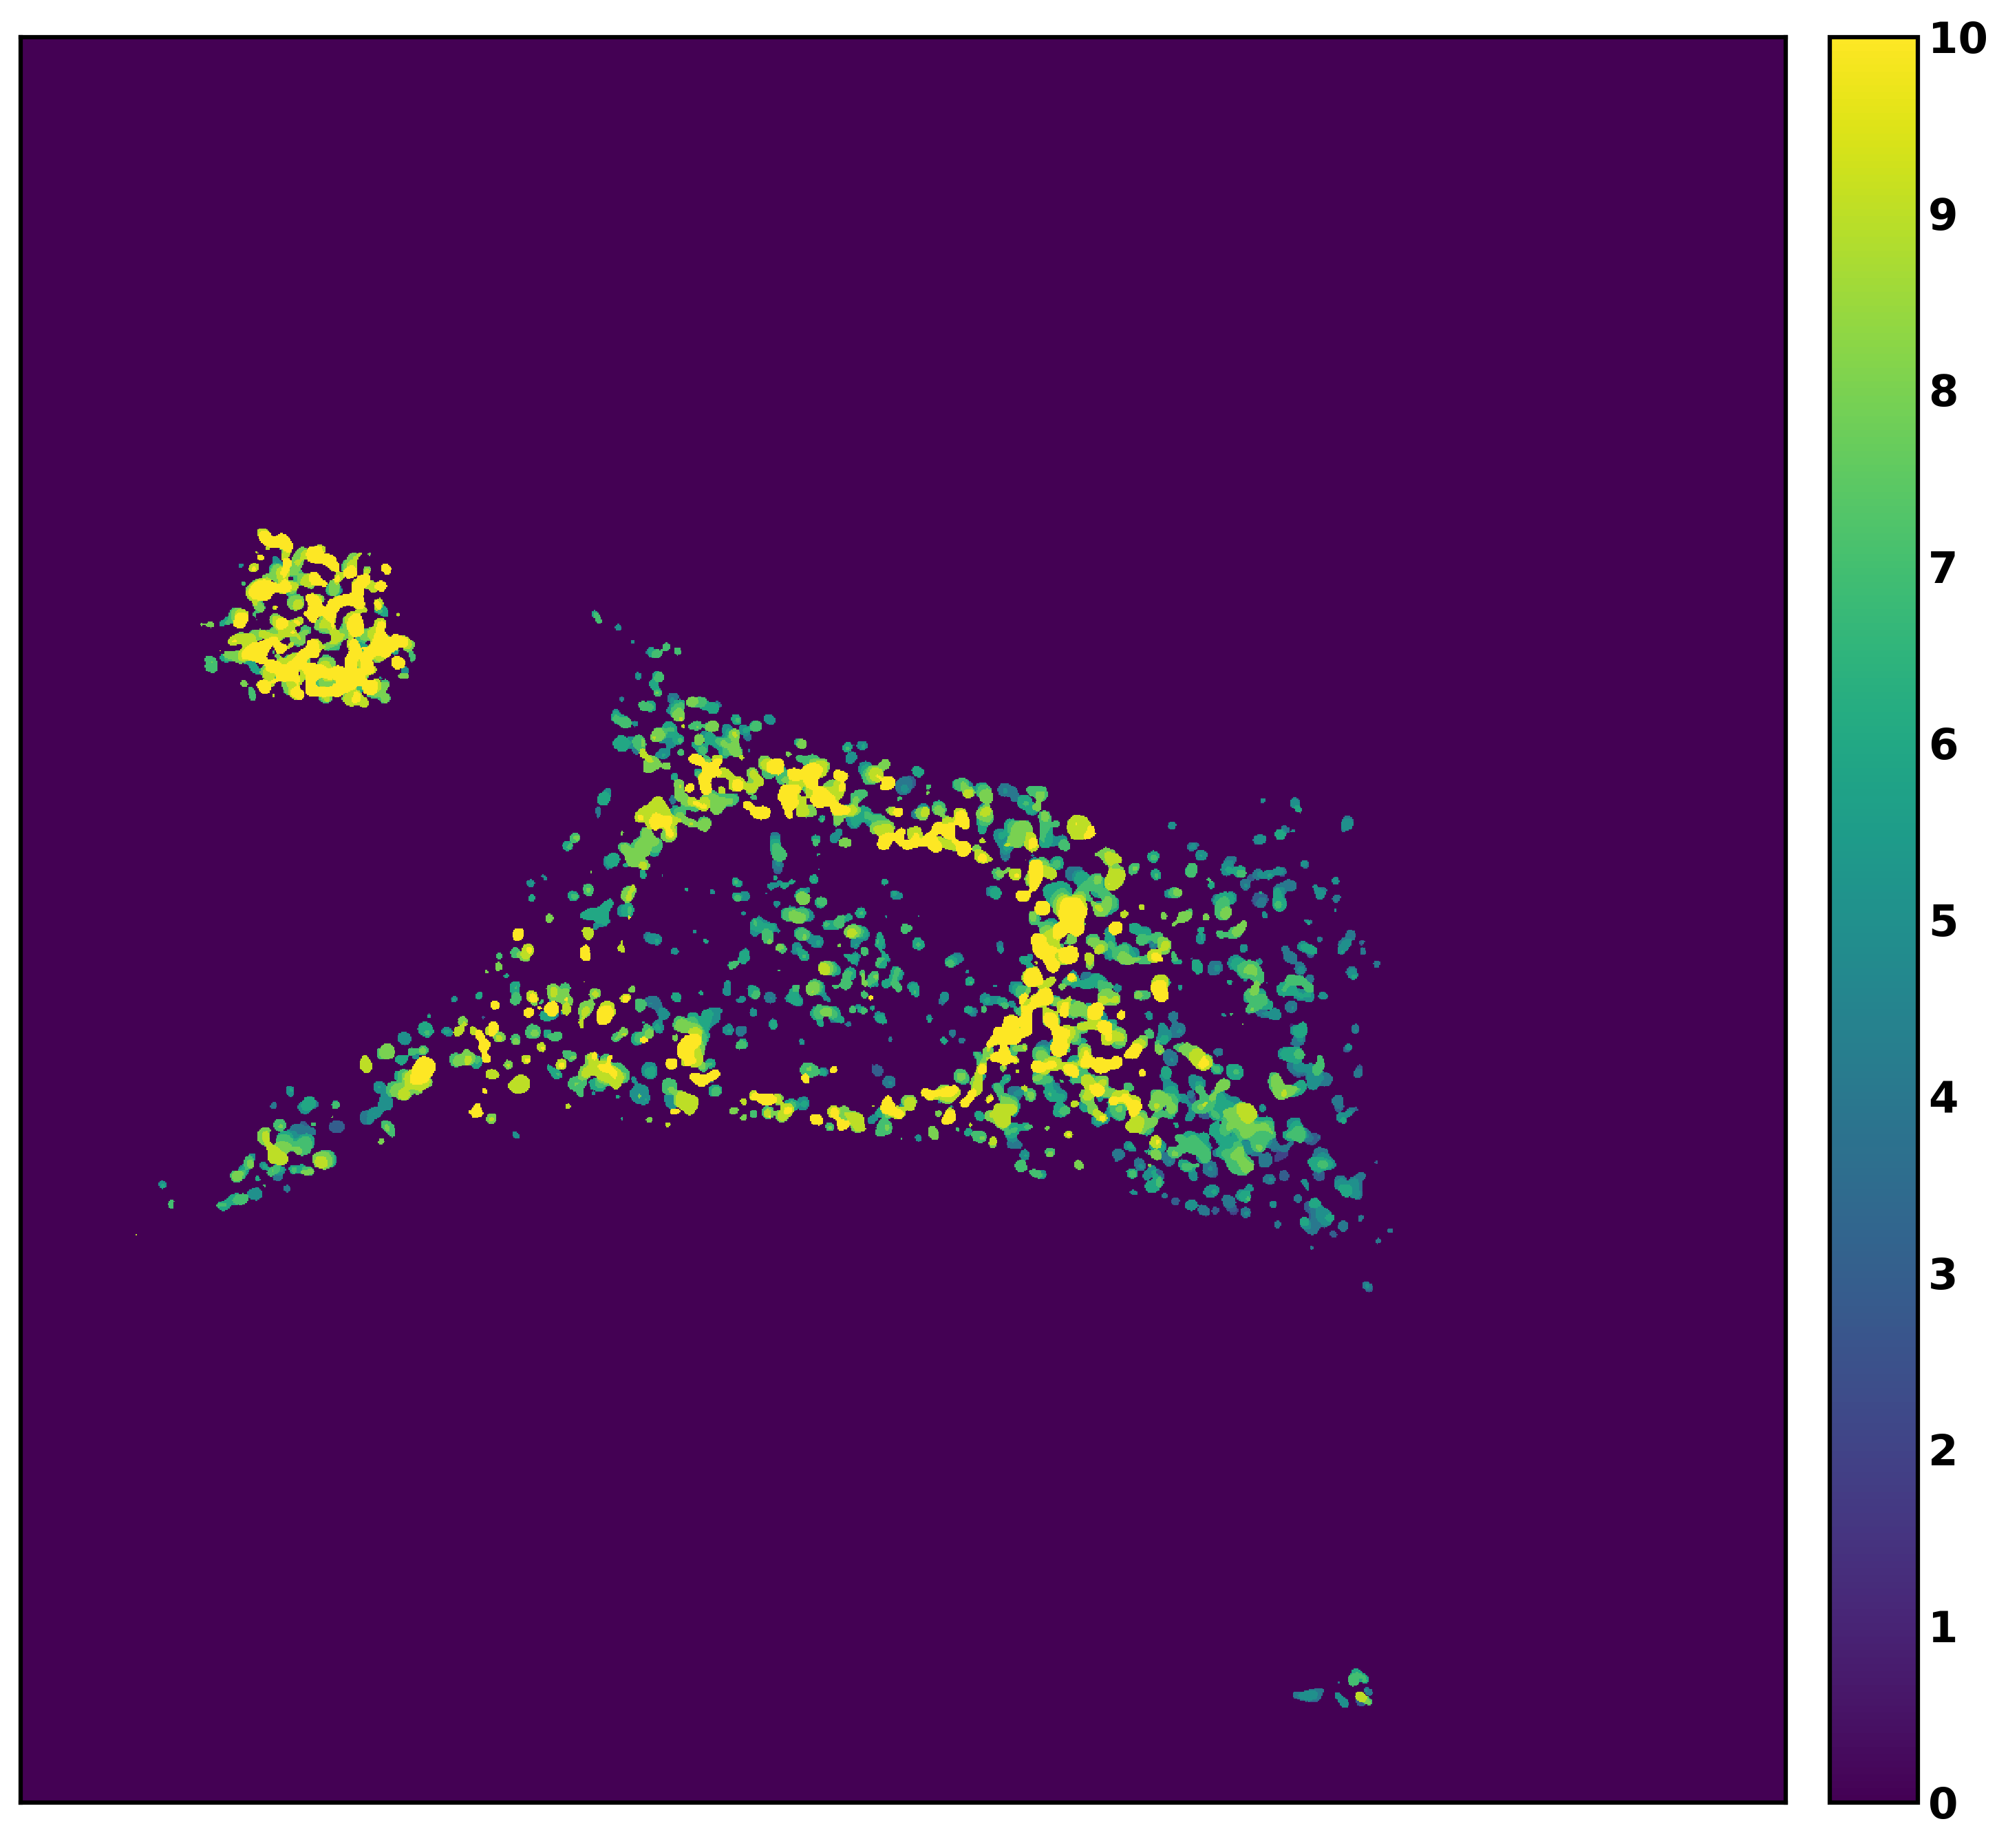
\includegraphics[width=0.32\textwidth]{figs/ch4figs/visual_analysis/global_outcomes/lyso/Flat_Con_2C=0_IsoData.png}}
	\subcaptionbox{Sample B depth project}{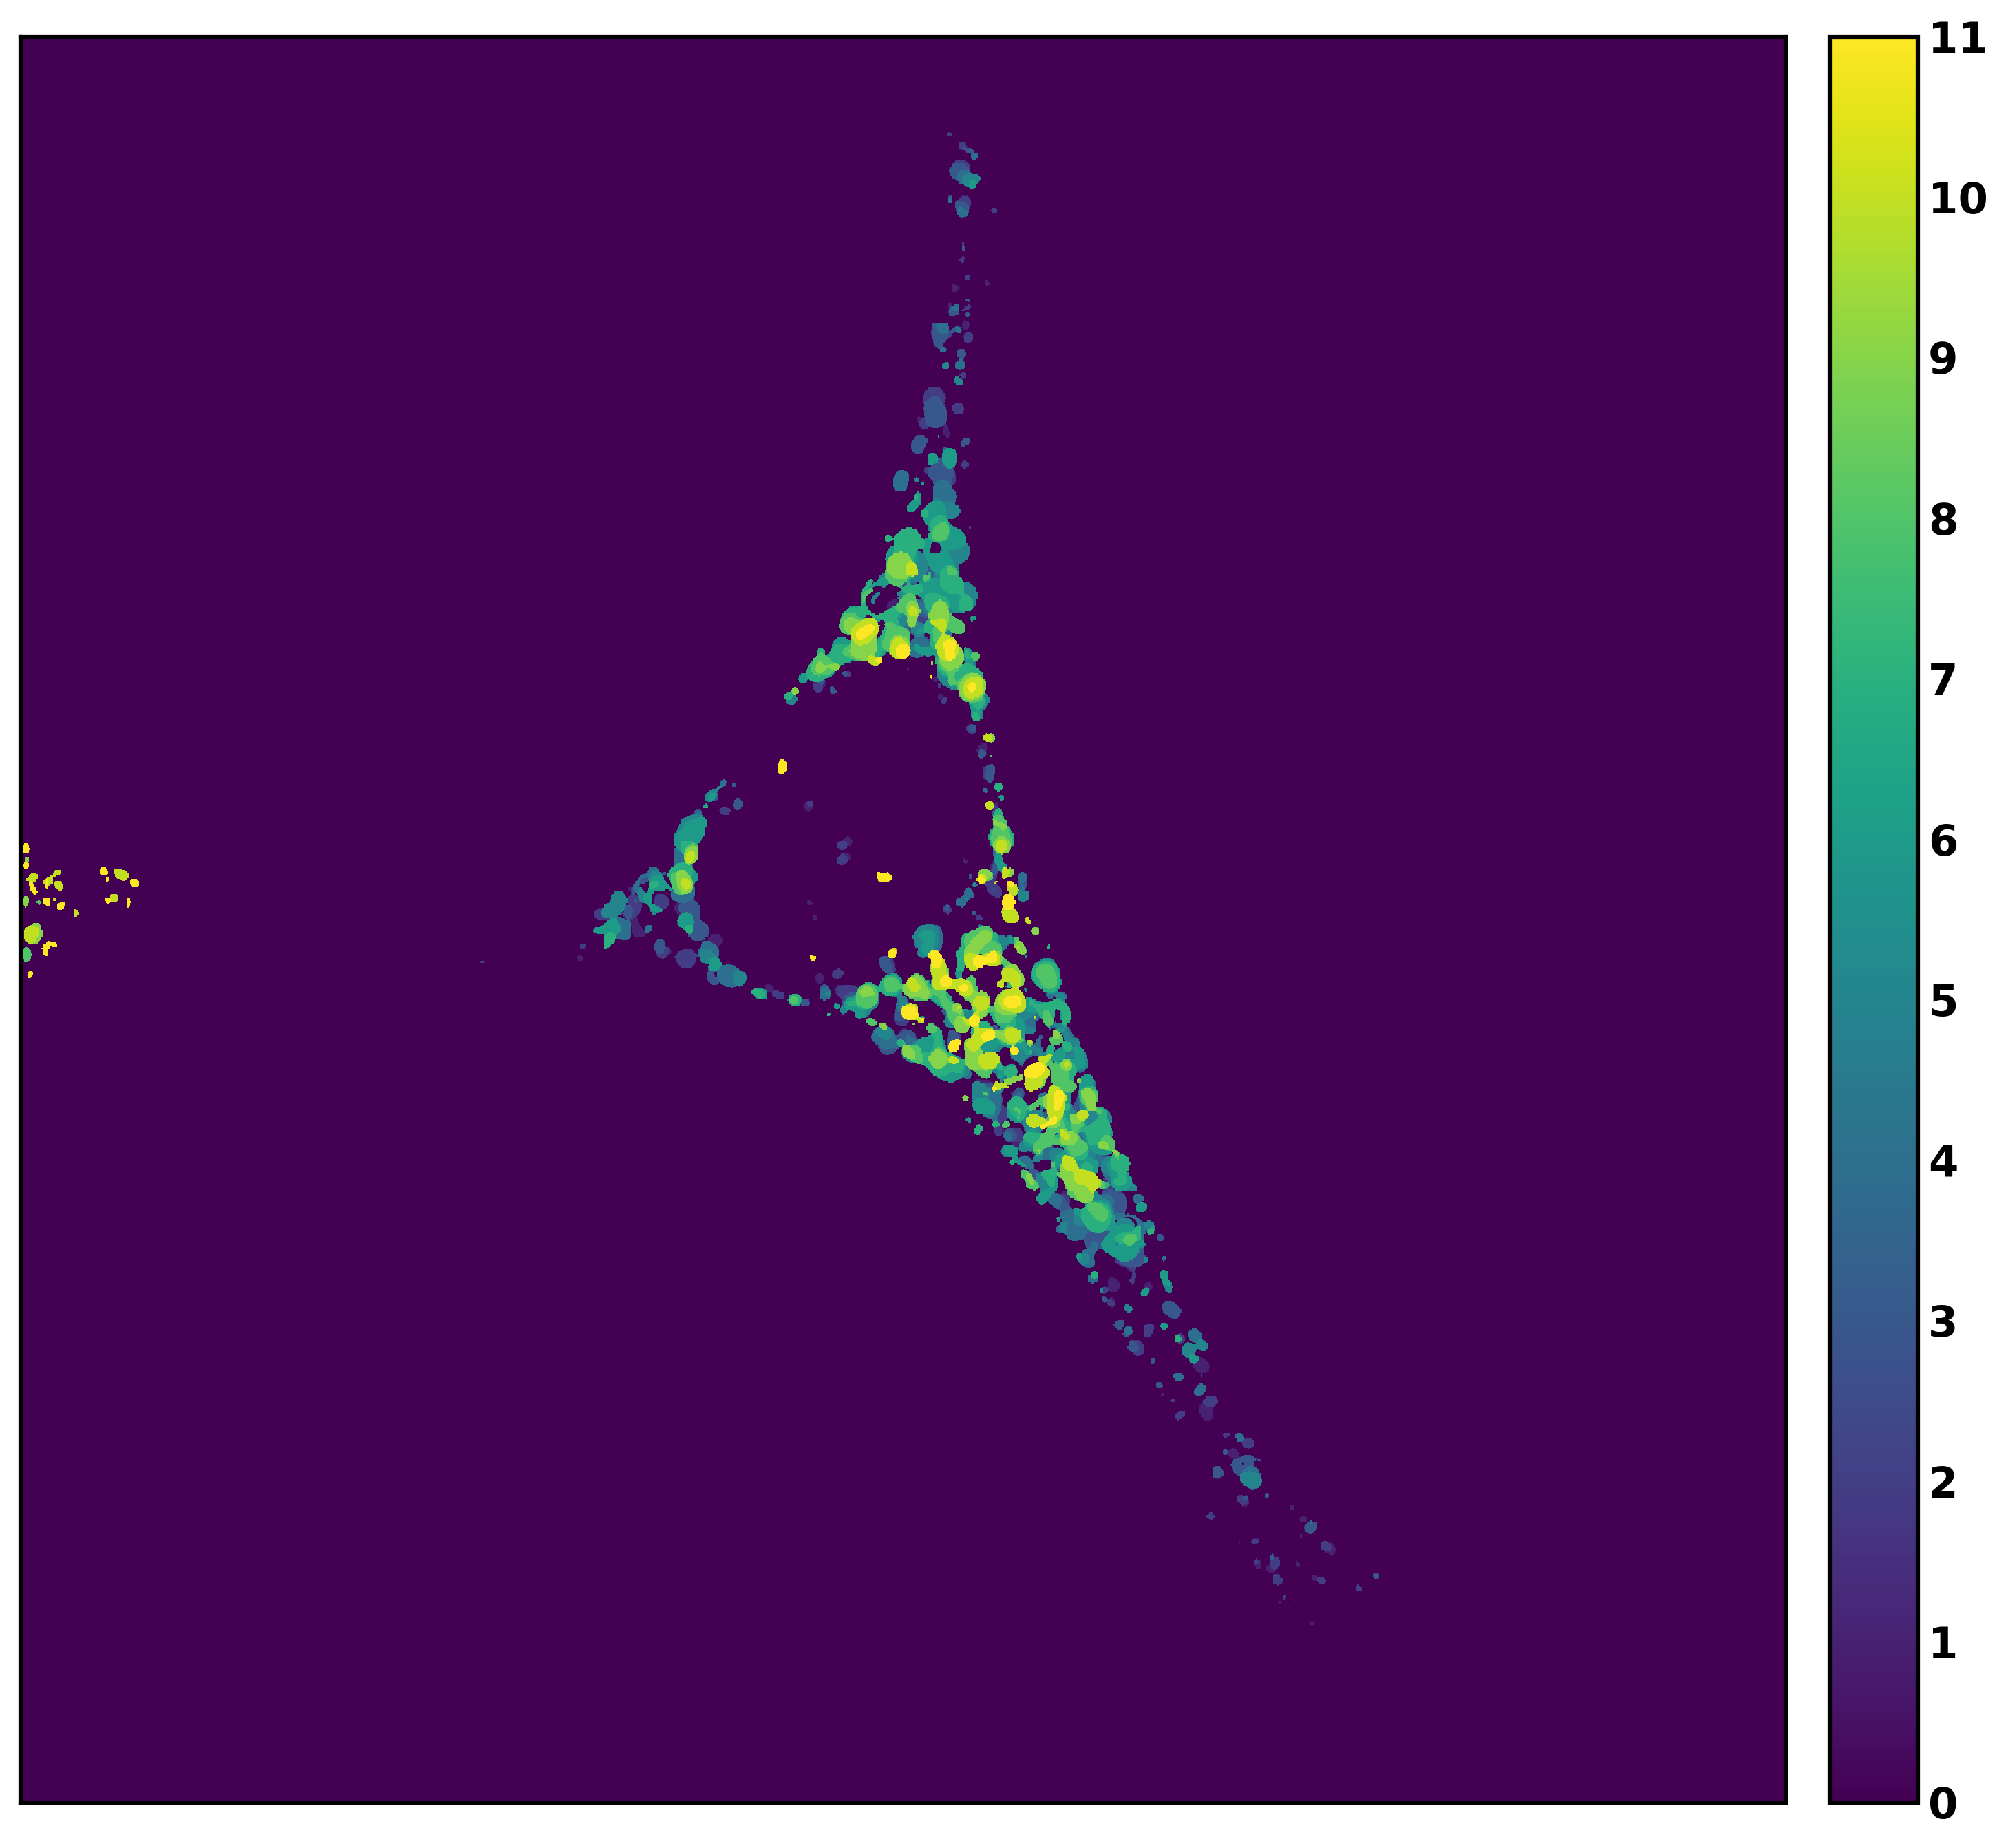
\includegraphics[width=0.32\textwidth]{figs/ch4figs/visual_analysis/global_outcomes/lyso/Flat_LML_3C=0_IsoData.png}}
	\subcaptionbox{Sample C depth project}{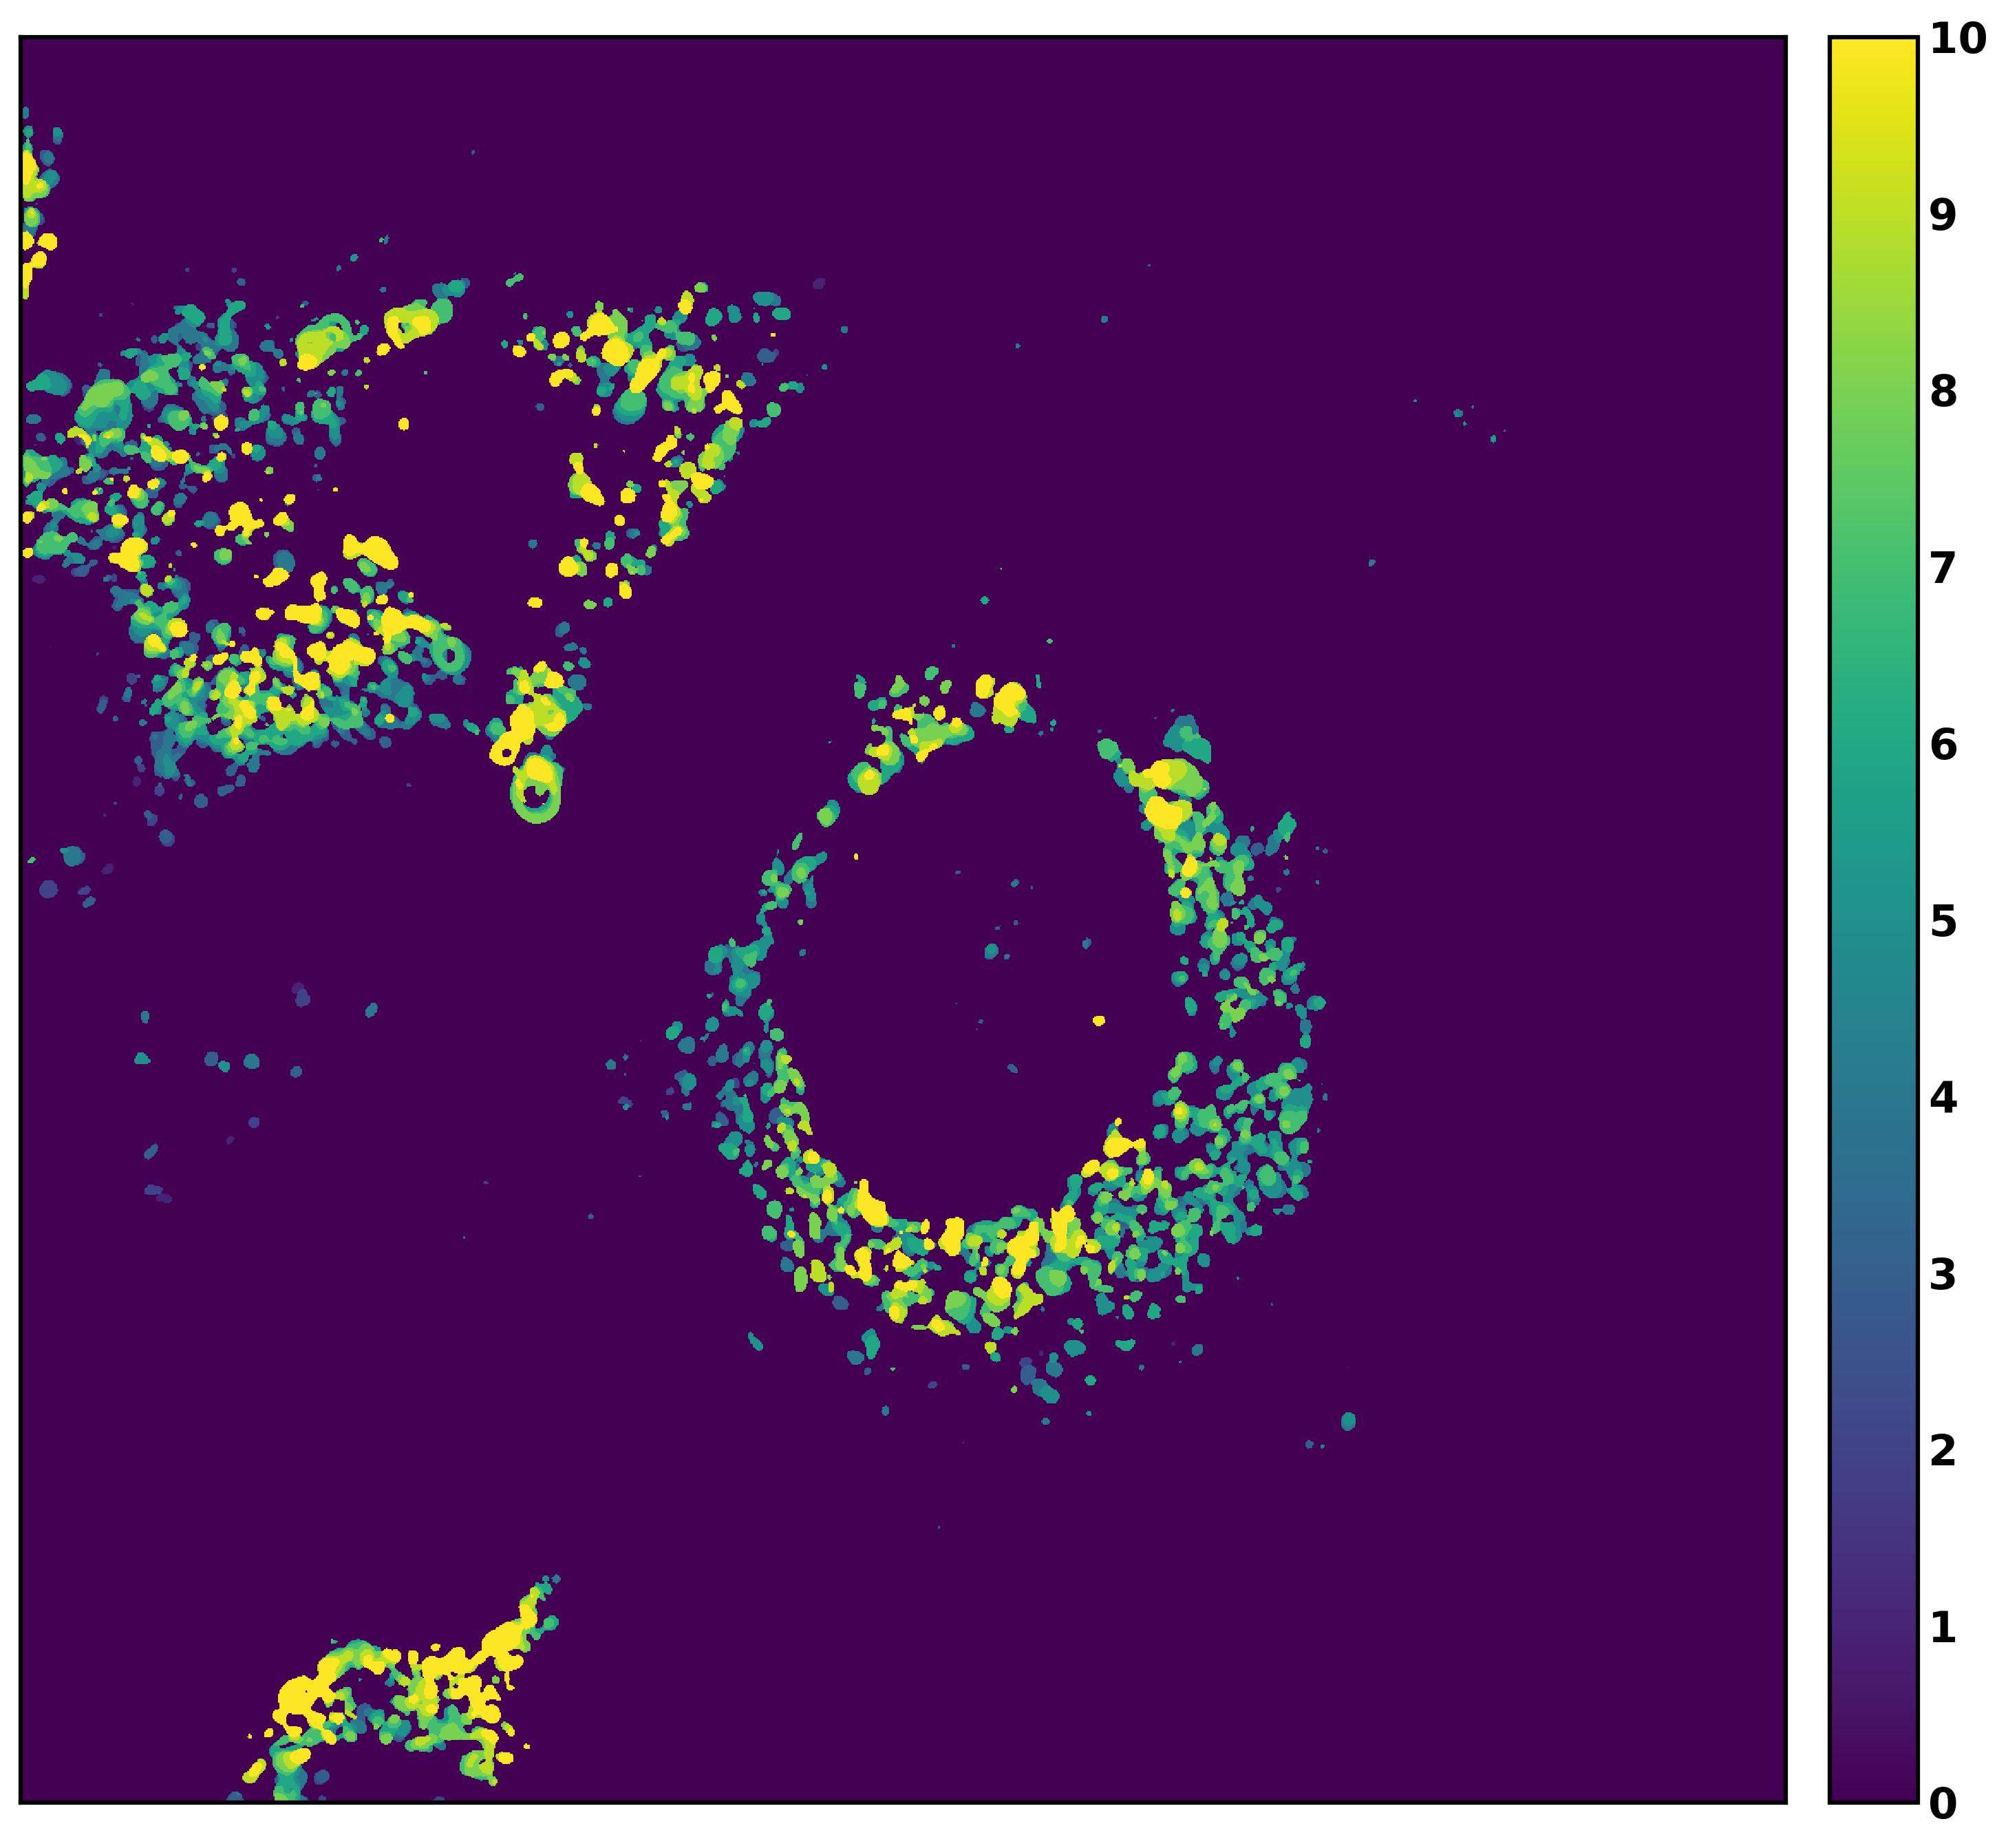
\includegraphics[width=0.32\textwidth]{figs/ch4figs/visual_analysis/global_outcomes/lyso/Flat_LML_4C=0_IsoData.png}}
	
	\subcaptionbox{Sample A RG centre slice overlay\label{subfig:lyso_rg_isodata_a}}{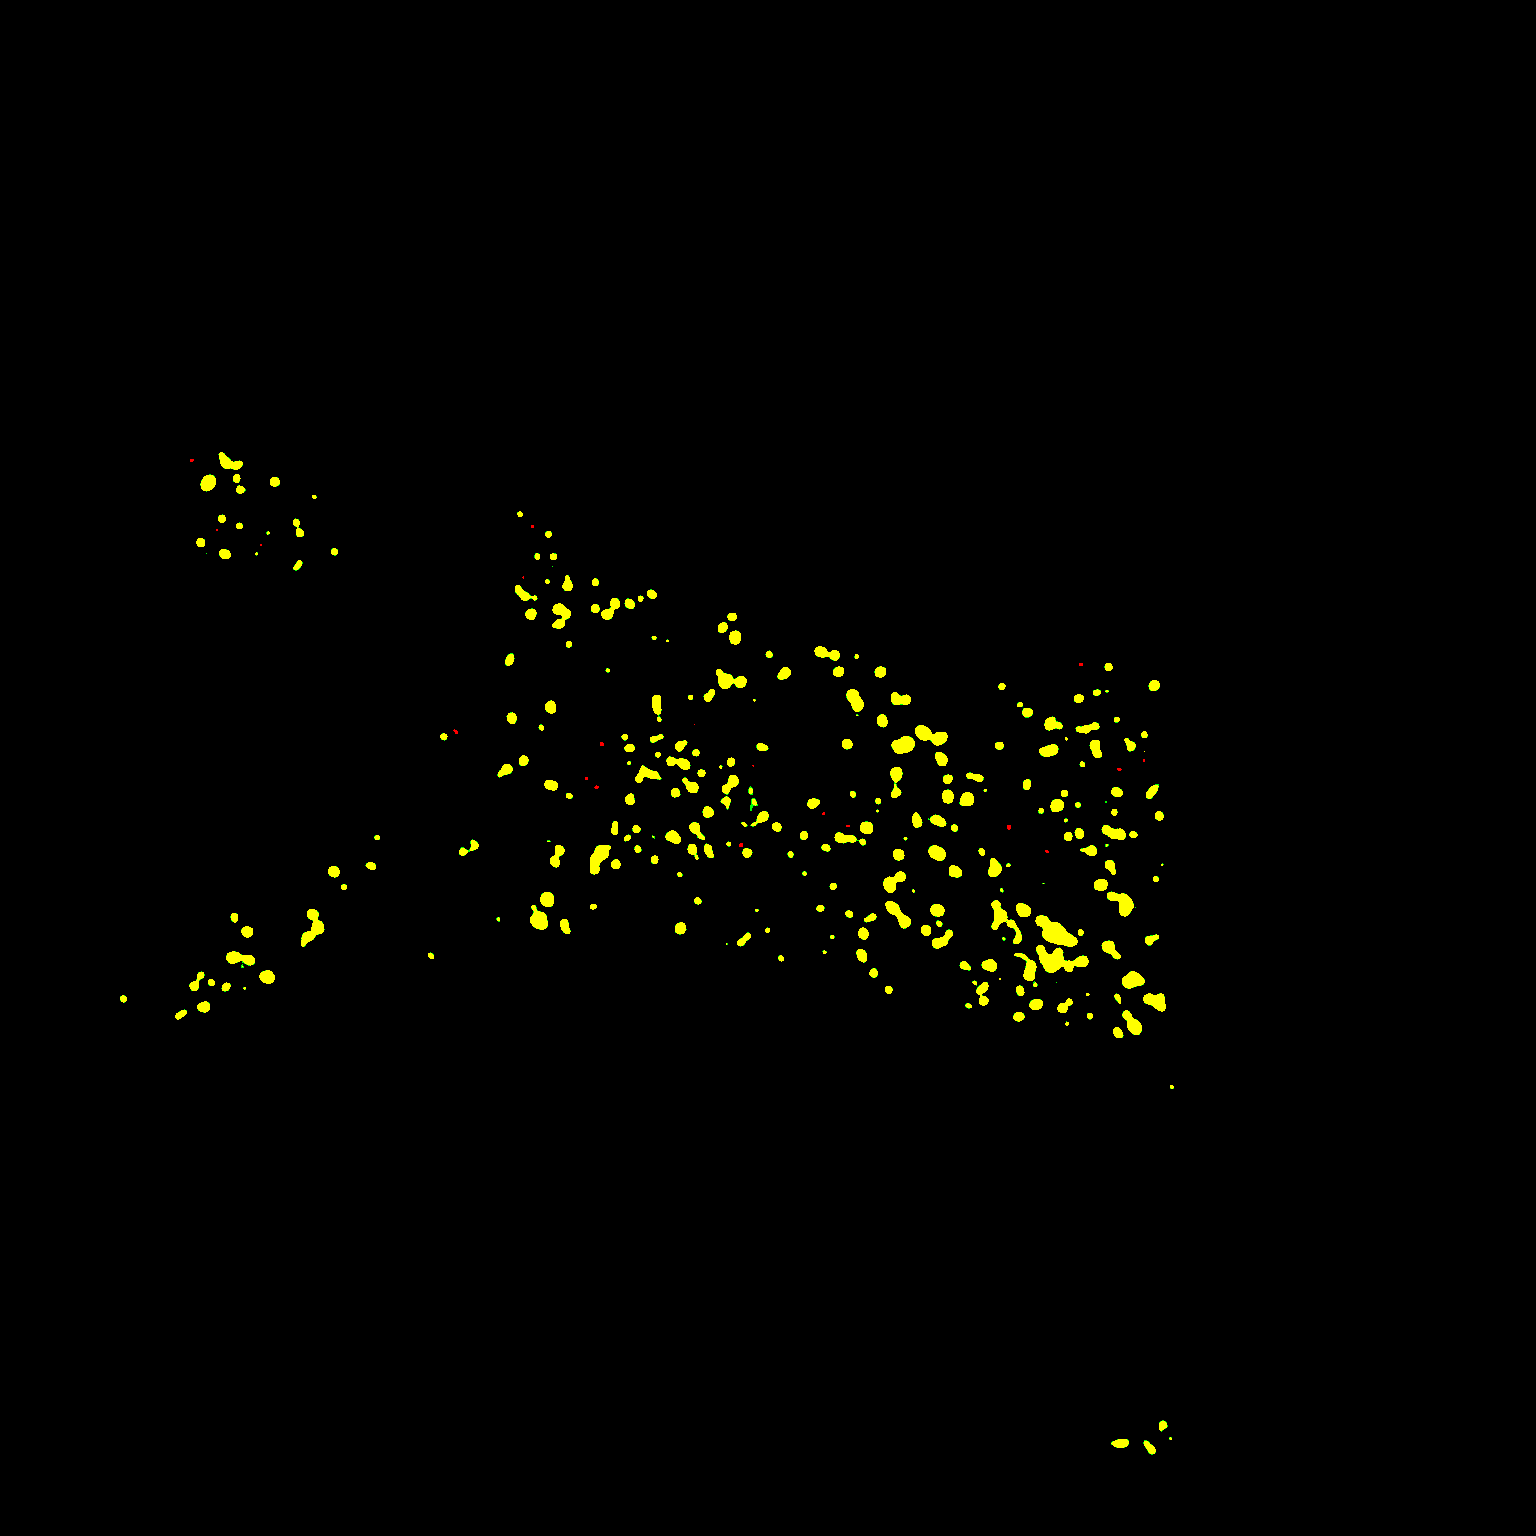
\includegraphics[width=0.32\textwidth]{figs/ch4figs/visual_analysis/global_outcomes/RG_IsoData_Con_2C=0.png}}
	\subcaptionbox{Sample B RG centre slice overlay\label{subfig:lyso_rg_isodata_b}}{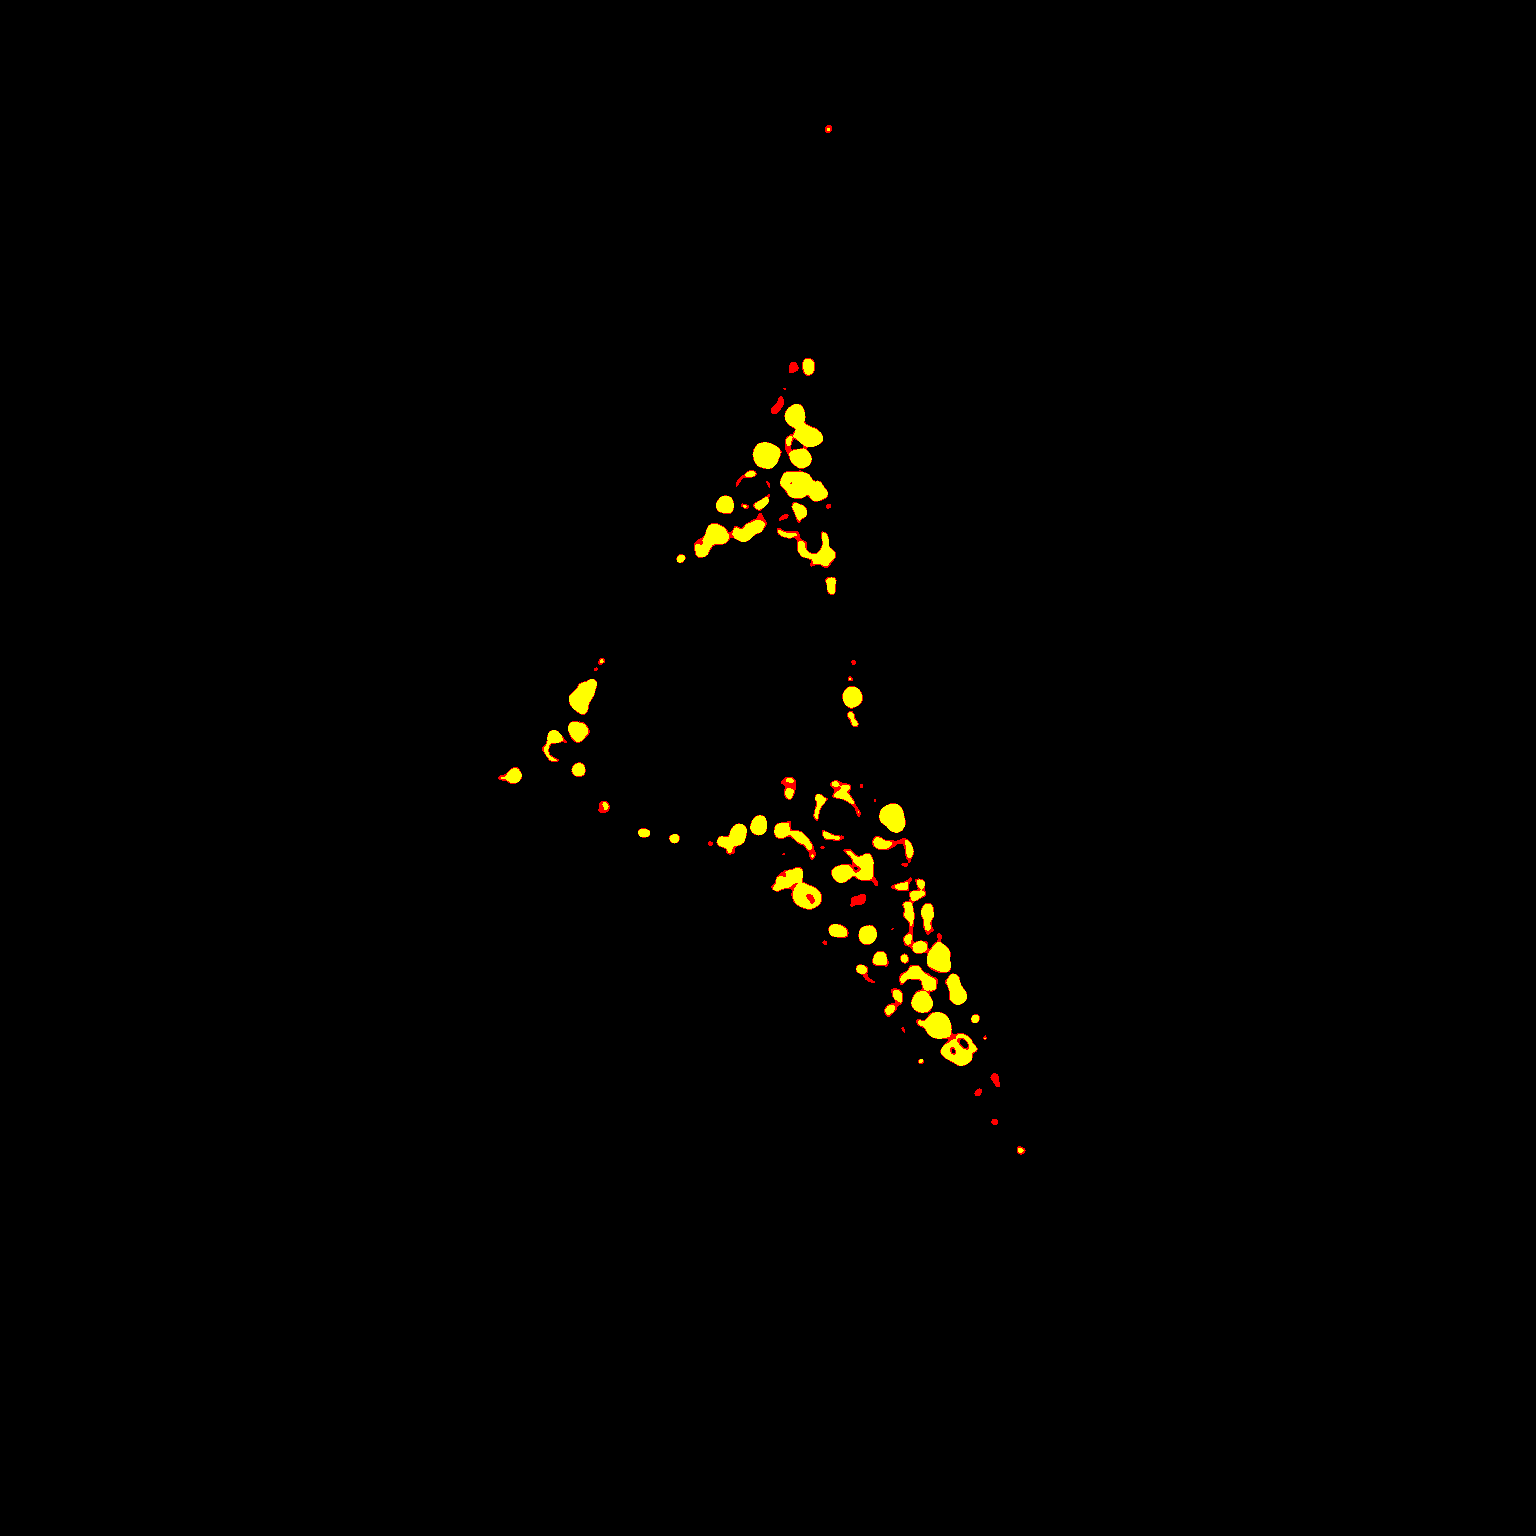
\includegraphics[width=0.32\textwidth]{figs/ch4figs/visual_analysis/global_outcomes/RG_IsoData_LML_3C=0.png}}
	\subcaptionbox{Sample C RG centre slice overlay\label{subfig:lyso_rg_isodata_c}}{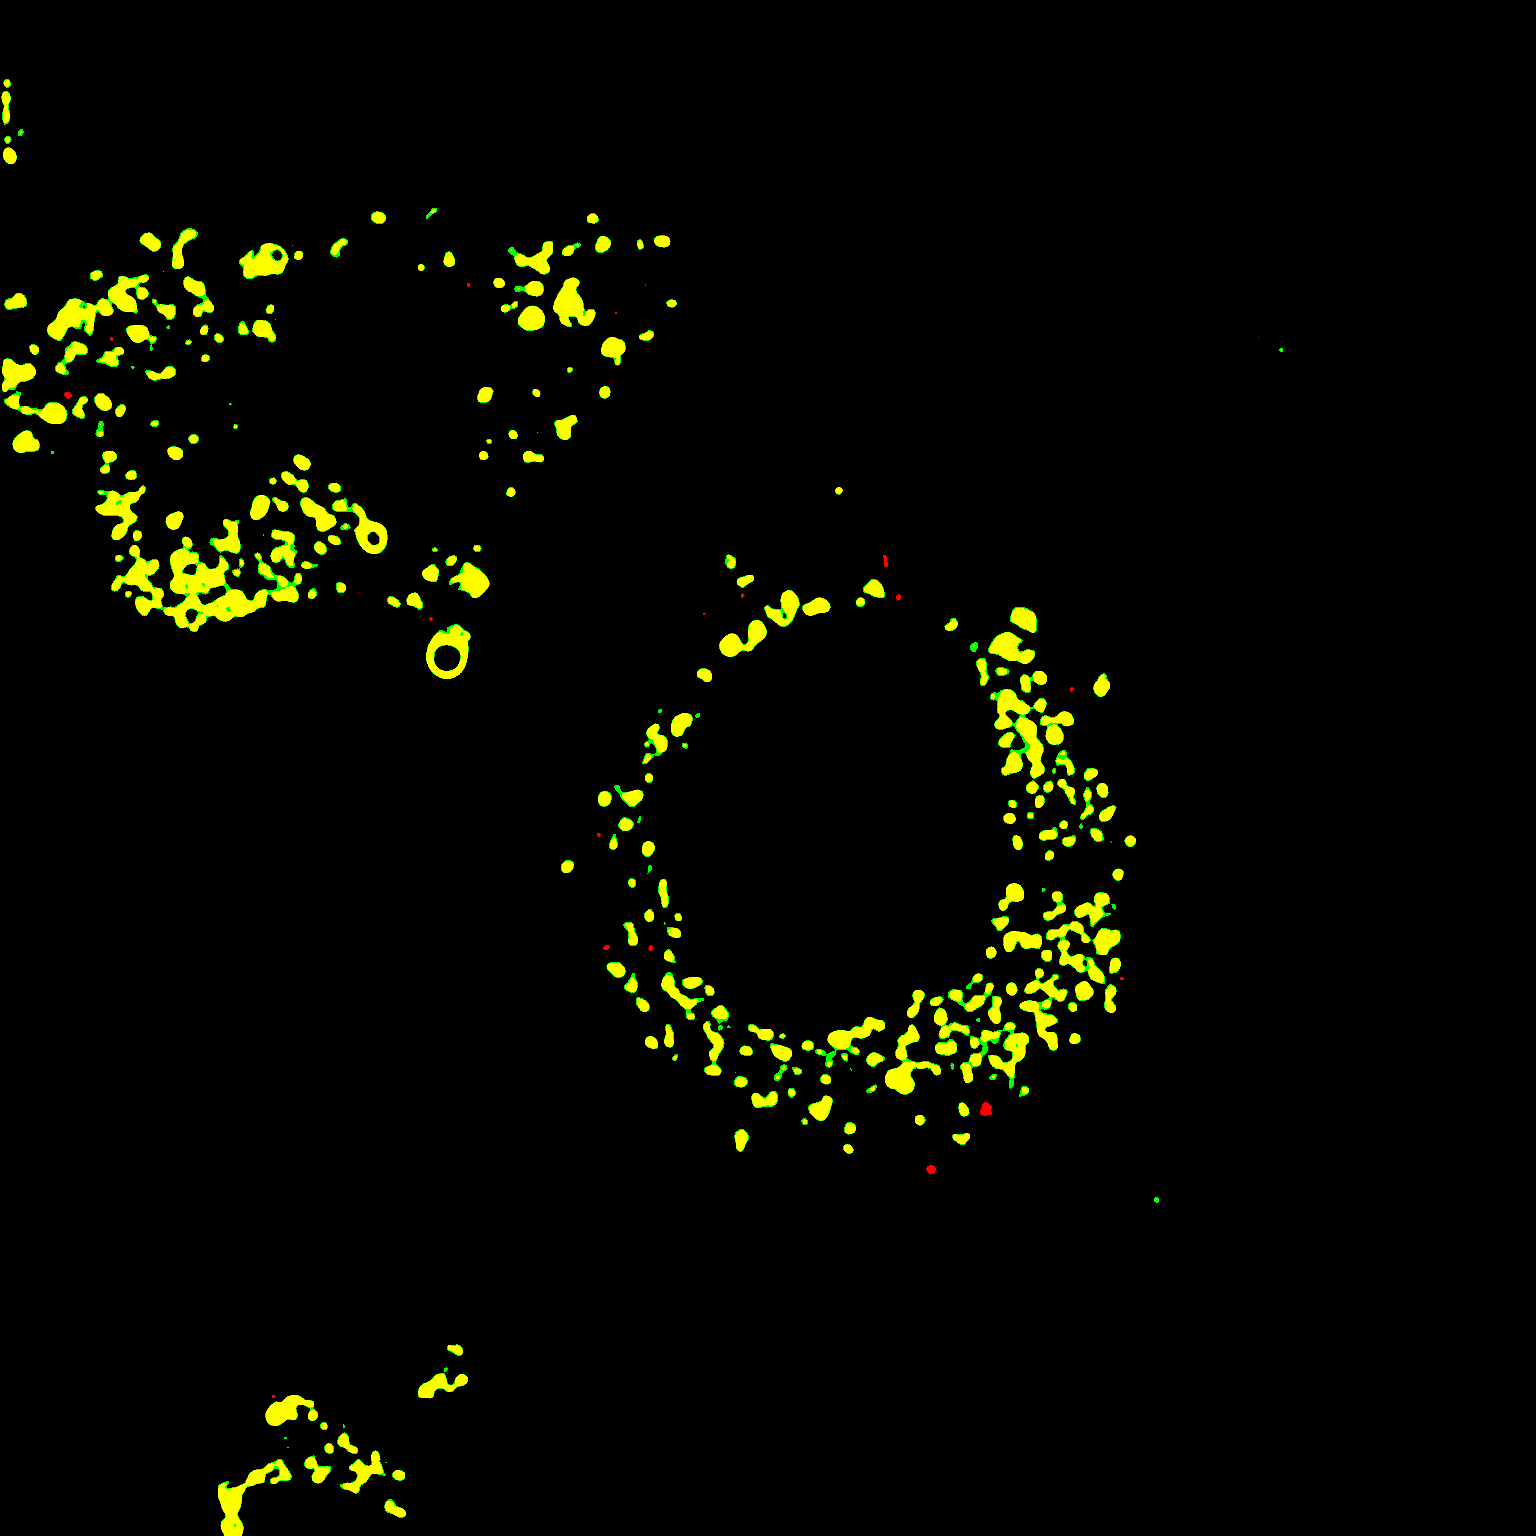
\includegraphics[width=0.32\textwidth]{figs/ch4figs/visual_analysis/global_outcomes/RG_IsoData_LML_4C=0.png}}
	
	\caption[Showcase of the lysosome samples binarised by the IsoData threshold and represented by depth projection and red-green overlay images.]{Showcase of the lysosome samples binarised by the IsoData threshold and represented by depth projection and centre slice red-green (RG) overlay images. The RG images overlay the IsoData binarisation as the red channel and the baseline binarisation as the green channel for a centre slice in the sample. Overlaps between foreground structures captured by both of these are presented as yellow.}
	\label{fig:lyso_isodata}
\end{figure}

\FloatBarrier
\paragraph{Otsu} The IsoData binarisations of the lysosome sample images are showcased in Figure \ref{fig:lyso_isodata}, which are represented by both depth projections and a red-green (RG) overlay of the IsoData and baseline binarisations for each sample's centre slice. It can be noted that observed results for Otsu are identical to those of IsoData; thus, all discussions in IsoData apply to Otsu.

\begin{figure}[h!]
	\centering
	\subcaptionbox{Sample A depth projection}{\includegraphics[width=0.32\textwidth]{figs/ch4figs/visual_analysis/global_outcomes/lyso/Flat_Con_2C=0_Otsu.png}}
	\subcaptionbox{Sample B depth projection}{\includegraphics[width=0.32\textwidth]{figs/ch4figs/visual_analysis/global_outcomes/lyso/Flat_LML_3C=0_Otsu.png}}
	\subcaptionbox{Sample C depth projection}{\includegraphics[width=0.32\textwidth]{figs/ch4figs/visual_analysis/global_outcomes/lyso/Flat_LML_4C=0_Otsu.png}}
	
	\subcaptionbox{Sample A RG centre slice overlay}{\includegraphics[width=0.32\textwidth]{figs/ch4figs/visual_analysis/global_outcomes/RG_Otsu_Con_2C=0.png}}
	\subcaptionbox{Sample B RG centre slice overlay}{\includegraphics[width=0.32\textwidth]{figs/ch4figs/visual_analysis/global_outcomes/RG_Otsu_LML_3C=0.png}}
	\subcaptionbox{Sample C RG centre slice overlay}{\includegraphics[width=0.32\textwidth]{figs/ch4figs/visual_analysis/global_outcomes/RG_Otsu_LML_4C=0.png}}
	
	\caption[Showcase of the lysosome samples binarised by the Otsu threshold and represented by depth projection and red-green overlay images.]{Showcase of the lysosome samples binarised by the Otsu threshold and represented by depth projection and centre slice red-green (RG) overlay images. The RG images overlay the Otsu binarisation as the red channel and the baseline binarisation as the green channel for a centre slice in the sample. Overlaps between foreground structures captured by both of these are presented as yellow.}
	\label{fig:lyso_moments}
\end{figure}

\paragraph{Overall}
Both the IsoData and Otsu methods produce good binarisations for all of the lysosome sample images while mitigating potential false joining present in the baseline binarisations for lysosome sample C. It must be acknowledged that the resultant binarisations for both methods are identical, but this does not imply that this threshold is their value. This is due to a range of possible threshold values being able to achieve the same binarisation, but with the size of this range dependent on the image; typically, the greater the contrast of the foreground structures against the background, the wider this range.  
\clearpage
\subsubsection{Local thresholding methods}
For the local thresholding methods the scores are shown in Table \ref{tab:lyso_local_ranks} with MidGrey and Bernsen being the top performing methods for the lysosome sample images.
\begin{table}[hb!]
	\centering
	\begin{tabular}{|c|c|c|c|c|}
		\hline
		\textbf{Method} & \textbf{Sample A} & \textbf{Sample B} & \textbf{Sample C} & \textbf{Mean score} \\
		\hline
		\textit{Baseline} & 5 & 4 & 4 & 4.3 \\
		\hline
		MidGrey & 2 & 3 & 2 & 2.3 \\
		\hline
		Bernsen & 1 & 3 & 2 & 2 \\
		\hline
		Mean & 1 & 2 & 2 & 1.6 \\
		\hline
		Median & 1 & 2 & 2 & 1.6 \\
		\hline
	\end{tabular}
	\caption{Rankings for each of the local thresholding methods for the lysosome sample images}
	\label{tab:lyso_local_ranks}
\end{table}
\FloatBarrier

\paragraph{MidGrey} The MidGrey binarisations of the lysosome sample images are showcased in Figure \ref{fig:lyso_midgrey}, which are represented by both depth projections and a red-green (RG) overlay of the MidGrey and baseline binarisations for each sample's centre slice. The performance for sample A is unusable, but the foreground structures are visually interpretable compared to the other methods. However, the excess noise in the background and major background inclusion are beyond recovery. For the sample, the results are significantly better than that of sample A, although there is a decrease in the foreground structure volume. Yet, the inclusion of less in-focus structures likely to be wholly out-of-focus is harder to differentiate due to sample B's limited contrast range. Regardless, this is how the presence of unlikely foreground structures and decreased structure volumes, potentially inducing structure fragmentation, make this unsuitable for most analyses beyond visual, where human nuance and judgement could compensate for these shortcomings. For sample C, there is excessive structure fragmentation and out-of-focus structure inclusion, rendering this binarisation unfit for any analysis, with the only benefit being an unreliable depiction of the structures' estimated positions.

\begin{figure}[h!]
	\centering
	\subcaptionbox{Sample A depth projection}{\includegraphics[width=0.32\textwidth]{figs/ch4figs/visual_analysis/local_outcomes/lyso/Flat_Con_2C=0_MidGrey.png}}
	\subcaptionbox{Sample B depth projection}{\includegraphics[width=0.32\textwidth]{figs/ch4figs/visual_analysis/local_outcomes/lyso/Flat_LML_3C=0_MidGrey.png}}
	\subcaptionbox{Sample C depth projection}{\includegraphics[width=0.32\textwidth]{figs/ch4figs/visual_analysis/local_outcomes/lyso/Flat_LML_4C=0_MidGrey.png}}
	
	\subcaptionbox{Sample A RG centre slice overlay}{\includegraphics[width=0.32\textwidth]{figs/ch4figs/visual_analysis/local_outcomes/RG_MidGrey_Con_2C=0.png}}
	\subcaptionbox{Sample B RG centre slice overlay}{\includegraphics[width=0.32\textwidth]{figs/ch4figs/visual_analysis/local_outcomes/RG_MidGrey_LML_3C=0.png}}
	\subcaptionbox{Sample C RG centre slice overlay}{\includegraphics[width=0.32\textwidth]{figs/ch4figs/visual_analysis/local_outcomes/RG_MidGrey_LML_4C=0.png}}
	
	\caption[Showcase of the lysosome samples binarised by the Otsu threshold and represented by depth projection and red-green overlay images.]{Showcase of the lysosome samples binarised by the MidGrey threshold and represented by depth projection and centre slice red-green (RG) overlay images. The RG images overlay the MidGrey binarisation as the red channel and the baseline binarisation as the green channel for a centre slice in the sample. Overlaps between foreground structures captured by both of these are presented as yellow.}
	\label{fig:lyso_midgrey}
\end{figure}

\FloatBarrier

\paragraph{Bernsen} The Bernsen binarisations of the lysosome sample images are showcased in Figure \ref{fig:lyso_bernsen}, which are represented by both depth projections and a red-green (RG) overlay of the Bernsen and baseline binarisations for each sample's centre slice. For sample A, this result is outright unusable for any purpose with the excessive inclusion of background intensities. Similarly to MidGrey, sample B suffers from an increased capture of less in-focus structures in the foreground, although with a slightly lower decrease in structure volumes, resulting in an unsuitable result for analysis. For sample C, the increase in the out-of-focus structures coupled with structure fragmentation renders these results unsuitable for any reliable analysis. 

\begin{figure}[h!]
	\centering
	\subcaptionbox{Sample A depth projection}{\includegraphics[width=0.32\textwidth]{figs/ch4figs/visual_analysis/local_outcomes/lyso/Flat_Con_2C=0_Bernsen.png}}
	\subcaptionbox{Sample B depth projection}{\includegraphics[width=0.32\textwidth]{figs/ch4figs/visual_analysis/local_outcomes/lyso/Flat_LML_3C=0_Bernsen.png}}
	\subcaptionbox{Sample C depth projection}{\includegraphics[width=0.32\textwidth]{figs/ch4figs/visual_analysis/local_outcomes/lyso/Flat_LML_4C=0_Bernsen.png}}
	
	\subcaptionbox{Sample A RG centre slice overlay}{\includegraphics[width=0.32\textwidth]{figs/ch4figs/visual_analysis/local_outcomes/RG_Bernsen_Con_2C=0.png}}
	\subcaptionbox{Sample B RG centre slice overlay}{\includegraphics[width=0.32\textwidth]{figs/ch4figs/visual_analysis/local_outcomes/RG_Bernsen_LML_3C=0.png}}
	\subcaptionbox{Sample C RG centre slice overlay}{\includegraphics[width=0.32\textwidth]{figs/ch4figs/visual_analysis/local_outcomes/RG_Bernsen_LML_4C=0.png}}
	
	\caption[Showcase of the lysosome samples binarised by the Bernsen threshold and represented by depth projection and red-green overlay images.]{Showcase of the lysosome samples binarised by the Bernsen threshold and represented by depth projection and centre slice red-green (RG) overlay images. The RG images overlay the Bernsen binarisation as the red channel and the baseline binarisation as the green channel for a centre slice in the sample. Overlaps between foreground structures captured by both of these are presented as yellow.}
	\label{fig:lyso_bernsen}
\end{figure}

\paragraph{Overall} It can be seen that all of the local thresholding methods perform badly for all of the lysosome sample images, with the top two performing methods providing good results only relativistically to the other methods. Regardless, none of these results appear to be viable for any analysis intending to produce reliability, in particular when attempting to generalise a method across a range of samples where a number of them are unseen. 

\FloatBarrier
\subsubsection{AHT method with varied bias applications}\label{sec:lyso_aht}
For the AHT evaluation, instead of several different methods, there are two types of biases which can be applied to the distribution: the IHH total volume bias (referred to as the IHH bias) and the Shrinking window bias (referred to as the Window bias). Both of these biases are discussed in Section \ref{sec:system_biases} where the Window bias is technically an umbrella of two variations, the Window width and Window mass weightings, and reference to either of these variations implies the application of the Window bias. From this, there are a total of six combinations of bias applications, which are:
\begin{multicols}{2}
	\begin{itemize}
		\item No biases applied.
		\item Application of only the Window width.
		\item Application of only the Window mass bias.
		\columnbreak
		\item Only the application of the IHH bias.
		\item Application of both the IHH and Window width biases.
		\item Application of both the IHH and Window mass biases.
	\end{itemize}
\end{multicols}


\begin{figure}[ht!]
	\centering
	\subcaptionbox{Distributions for Sample A\label{subfig:ihh_lyso_a}}{\includegraphics[width=0.32\textwidth]{figs/ch4figs/visual_analysis/aht_outcomes/Distributions/IHH_Distrib_Con_2C=0.png}}
	\subcaptionbox{Distributions for Sample B\label{subfig:ihh_lyso_b}}{\includegraphics[width=0.32\textwidth]{figs/ch4figs/visual_analysis/aht_outcomes/Distributions/IHH_Distrib_LML_3C=0.png}}
	\subcaptionbox{Distributions for Sample C\label{subfig:ihh_lyso_c}}{\includegraphics[width=0.32\textwidth]{figs/ch4figs/visual_analysis/aht_outcomes/Distributions/IHH_Distrib_LML_4C=0.png}}
	\caption[The IHH and smoothed IHH gradient distributions for the lysosome samples.]{The IHH and smoothed IHH gradient distributions for the lysosome samples with the top and bottom line plots depicting the former and latter distributions, respectively.}
	\label{fig:lyso_ihh_distribs}
\end{figure}
With each influencing the shape of the distribution used to calculate the centroid used as the high threshold, in the case of the IHH bias, or the weighting for the weighted mean of centroid values calculated for incrementally shrinking windows of the AHT distributions that reduce the high threshold intensities upper bound.\par For the three lysosome sample intensity images, the Hysteresis foreground voxel count for a range of intensity values, referred to as the IHH, as well as the smoothed gradient representation of the IHH, are shown in Figure \ref{fig:lyso_ihh_distribs}. From these distributions, certain image characteristics can be inferred, such as the gradual decline in the IHH distribution of sample A, Figure \ref{fig:lyso_ihh_distribs} (\subref{subfig:ihh_lyso_a}), has a relatively high contrast given that the maximum foreground voxel count is about $\num{390e3}$. In contrast, the minimum count is roughly $\num{360e3}$. This implies that about $92\%$ of the foreground voxels are already included at the maximum high threshold intensity. In contrast, the slope implies a wide dispersal of foreground voxels across the remaining range, but the total volume is small. An edge case behaviour can be seen for sample B, Figure \ref{fig:lyso_ihh_distribs} (\subref{subfig:ihh_lyso_b}),  where the IHH distribution has a sudden drop to zero foreground voxels between the high threshold intensities of $150$ and $200$ but this is due to the low maximum intensity of sample B, as shown in Figure \ref{fig:lysosome_raw} (\subref{subfig:lyso_sampl_orig_b}), but this induces a false peak in the gradient at that value. The repercussions of this will be explored further after the binarisation rankings for the different bias combinations shown in table \ref{tab:lyso_aht}.

\begin{table}
	\centering
	\begin{tabular}{|c|c|c|c|c|c|}
		\hline
		IHH bias applied & Window bias applied & Sample A & Sample B & Sample C & Mean Rank \\
		\hline
		No & None & 3 & 1 & 4 & 2.6 \\
		\hline
		No & Window width & 2 & 3 & 4 & 3 \\
		\hline
		No & Window mass & 2 & 1 & 4 & 2.3 \\
		\hline
		Yes & None & 2 & 3 & 4 & 3 \\
		\hline
		Yes & Window width & 2 & 3 & 3 & 2.6 \\
		\hline
		Yes & Window mass & 2 & 3 & 3 & 2.6 \\
		\hline
		\textit{Baseline} & & 5 & 4 & 4 & 4.3 \\
		\hline
	\end{tabular}
	\caption{Rankings of the AHT threshold outcomes for the three samples with different combinations of the IHH and Window biases}
	\label{tab:lyso_aht}
\end{table}
Table \ref{tab:lyso_aht} shows that the overall performance for several samples was not impressive, with no mean scores exceeding $3$. This is because the determined low threshold value is too low and has induced the excessive joining of structures in the binarisations. An example of this is shown in Figure \ref{fig:lyso_aht_select} (\subref{subfig:aht_lyso_joins}) where the current structures have been selected through the high threshold, represented by the yellow regions, but the extended volumes of these regions, inducing joining, is shown by the red regions connected to the yellow. The repercussions of the false peak in the gradient distribution are shown in Figure \ref{fig:lyso_aht_select} (\subref{subfig:aht_lyso_vanished_b}) where this has resulted in a high threshold exceeding the maximum voxel intensities within sample B.\par

\begin{figure}[h!]
	\subcaptionbox{No biases for sample A\label{subfig:aht_lyso_joins}}{\includegraphics[width=0.32\textwidth]{figs/ch4figs/visual_analysis/aht_outcomes/lyso/AHTv0w0_Con_2C=0.png}}
	\subcaptionbox{No biases for sample B\label{subfig:aht_lyso_vanished_b}}{\includegraphics[width=0.32\textwidth]{figs/ch4figs/visual_analysis/aht_outcomes/lyso/AHTv0w0_LML_3C=0.png}}
	\subcaptionbox{IHH bias for sample B\label{subfig:aht_lyso_good_b}}{\includegraphics[width=0.32\textwidth]{figs/ch4figs/visual_analysis/aht_outcomes/lyso/AHTv1w0_LML_3C=0.png}}
	\caption{RG overlay images of the baseline and AHT binarisations for select bias combinations and lysosome sample images.}
	\label{fig:lyso_aht_select}
\end{figure}

Finally, the set of all high threshold values for each sample's bias combination is shown in Figure \ref{fig:lyso_aht_distribs} where the distributions shown are inversions of the gradient distributions in Figure \ref{fig:lyso_ihh_distribs}. 

\begin{figure}
	\centering
	\subcaptionbox{Sample A gradient distributions}{\includegraphics[width=\textwidth]{figs/ch4figs/visual_analysis/aht_outcomes/Distributions/AHT_Distrib_Con_2C=0.png}}
	\subcaptionbox{Sample B gradient distributions \label{subfig:lyso_aht_b}}{\includegraphics[width=\textwidth]{figs/ch4figs/visual_analysis/aht_outcomes/Distributions/AHT_Distrib_LML_3C=0.png}}
	\subcaptionbox{Sample C gradient distributions}{\includegraphics[width=\textwidth]{figs/ch4figs/visual_analysis/aht_outcomes/Distributions/AHT_Distrib_LML_4C=0.png}}
	\caption{The smoothed inverted gradient distributions, derived from the inversion of the gradient distributions shown in Figure \ref{fig:lyso_ihh_distribs}, with the centroids appropriate for each bias application. The inverted gradient distribution post-application of the IHH bias is also shown as this is the distribution that is used for the IHH bias applied high thresholds}
	\label{fig:lyso_aht_distribs}
\end{figure}


\paragraph{Overall}
From the results shown, the AHT biases appear to respond well to high threshold selection while capturing fewer out-of-focus structures than the foreground. However, this is heavily constrained by the low threshold value being too low. The ideal biases for the lysosome type structures would be the IHH bias in isolation as it mitigates the edge case found in sample B which can be seen both in Figure \ref{fig:lyso_aht_select} (\subref{subfig:aht_lyso_good_b}) and in the ``Inverted Gradient Distribution with IHH bias applied'' in Figure \ref{fig:lyso_aht_distribs} (\subref{subfig:lyso_aht_b}) where the distribution plateaus at zero instead of peaking removing it's contribution to the high threshold determination.




\FloatBarrier

\subsection{Autophagosome structures}
The autophagosome structures captured in the autophagosome channel of the sample intensity images, shown in Figure \ref{fig:raw_samples_rgb}, are depicted in Figure \ref{fig:autophagosome_raw} where the autophagosome sample images are depicted with both MIP and centre slice representations. Contrast enhancement has been applied for samples B and C, Figure \ref{fig:autophagosome_raw} (\subref{subfig:auto_sampl_ec_a} \& \subref{subfig:auto_sampl_ec_b}), to visualise the large quantity of background noise present in these images which is going to be detrimental to thresholding methods' binarisation. \paragraph{Specific autophagosome sample observations:} The number of bright structures effectively contrasting against this background noise in autophagosome sample A, Figure \ref{subfig:auto_sampl_orig_a}, while increasing the likelihood that these dimmer surrounding structures will be binarised as foreground but also lowers the visual certainty whether these are the actual foreground structures. In autophagosome sample B, Figure \ref{subfig:auto_sampl_orig_b}, there is a more significant number of structures with a lower maximum intensity, but, based on the contrast-enhanced visualisation in Figure \ref{subfig:auto_sampl_ec_b}, the background noise appears to be less dense than in sample A. Autophagosome sample C appears to be a well-imaged specimen with minor quantities of background noise and bright structures contrasting against the background which is believed to belong to the foreground.

\begin{figure}[ht!]
	\centering
	\subcaptionbox{Sample A intensity MIP image\label{subfig:auto_sampl_orig_a}}{\includegraphics[width=0.3\textwidth]{figs/ch4figs/visual_analysis/raw_samples/MAX_Con_2C=1.png}}
	\subcaptionbox{Sample B intensity MIP image\label{subfig:auto_sampl_orig_b}}{\includegraphics[width=0.3\textwidth]{figs/ch4figs/visual_analysis/raw_samples/MAX_LML_3C=1.png}}
	\subcaptionbox{Sample C intensity MIP image\label{subfig:auto_sampl_orig_c}}{\includegraphics[width=0.3\textwidth]{figs/ch4figs/visual_analysis/raw_samples/MAX_LML_4C=1.png}}
	\subcaptionbox{Sample A centre slice with EC\label{subfig:auto_sampl_ec_a}}{\includegraphics[width=0.3\textwidth]{figs/ch4figs/visual_analysis/raw_samples/Centre_Con_2C=1.png}}
	\subcaptionbox{Sample B centre slice with EC\label{subfig:auto_sampl_ec_b}}{\includegraphics[width=0.3\textwidth]{figs/ch4figs/visual_analysis/raw_samples/Centre_LML_3C=1.png}}
	\subcaptionbox{Sample C centre slice\label{subfig:auto_sampl_ec_c}}{\includegraphics[width=0.3\textwidth]{figs/ch4figs/visual_analysis/raw_samples/Centre_LML_4C=1.png}}
	\caption[Image panel of the autophagosome sample intensity images used in binarisation.]{Image panel for the autophagosome channel of the sample images. The first row is the MIP representations, and the second is the intensity images' centre slices before binarisation. Contrast enhancement (EC) has been applied to the centre slices of samples A and B to help visualise the noise and does not factor into the binarisation outcomes.}
	\label{fig:autophagosome_raw}
\end{figure}

\FloatBarrier
\paragraph{Autophagosome baseline:} 
The showcase of the autophagosome baseline images is shown in Figure \ref{fig:auto_baseline} and is binarised from the autophagosome intensity images in Figure \ref{fig:autophagosome_raw}. From the depth projections and binarised centre slices shown, it can be seen that neither the number of structures nor the volume of said structures is large for sample A. While certainty over this being an accurate representation of the actual structures that were imaged, the background noise renders this indiscernible. Sample B produces clearer structures with only small, sparse, speckle-like structures across the background with a low foreground structure count. Sample C depicts a distinct set of foreground structures with low out-of-focus structures and reasonable quantities of structural joins. 
\begin{figure}[ht!]
	\centering
	\subcaptionbox{Sample A}{\includegraphics[width=0.28\textwidth]{figs/ch4figs/visual_analysis/raw_samples/Flat_Con_2C=1_Hyst.png}}
	\subcaptionbox{Sample B}{\includegraphics[width=0.28\textwidth]{figs/ch4figs/visual_analysis/raw_samples/Flat_LML_3C=1_Hyst.png}}
	\subcaptionbox{Sample C}{\includegraphics[width=0.28\textwidth]{figs/ch4figs/visual_analysis/raw_samples/Flat_LML_4C=1_Hyst.png}}
	\subcaptionbox{Sample A centre slice}{\includegraphics[width=0.28\textwidth]{figs/ch4figs/visual_analysis/raw_samples/Hyst_Con_2C=1.png}}
	\subcaptionbox{Sample B centre slice\label{subfig:auto_centre_base}}{\includegraphics[width=0.28\textwidth]{figs/ch4figs/visual_analysis/raw_samples/Hyst_LML_3C=1.png}}
	\subcaptionbox{Sample C centre slice}{\includegraphics[width=0.28\textwidth]{figs/ch4figs/visual_analysis/raw_samples/Hyst_LML_4C=1.png}}
	\caption[Showcase of the baseline binarisations for each autophagosome sample image.]{Showcase of the baseline binarisations for each autophagosome sample image, generated through manually tuned Hysteresis thresholding and depicted using depth projection and binary centre slice images with the former in the top row and the latter in the bottom row. Figure \ref{fig:autophagosome_raw} shows the respective autophagosome sample intensity images.}
	\label{fig:auto_baseline}
\end{figure}
\FloatBarrier

\subsubsection{Global thresholding methods}
The scoring of each thresholding method's binarisations of the autophagosome sample intensity images are shown in Table \ref{tab:auto_global_ranks} where the top performing methods are MaxEntropy and RenyiEntropy, both of which are discussed in Section \ref{sec:max_renyi_entr}.
\begin{table}[hb!]
	\centering
	\begin{tabular}{|c|c|c|c|c|}
		\hline
		\textbf{Method} & \textbf{Sample A} & \textbf{Sample B} & \textbf{Sample C} & \textbf{Mean score}\\
		\hline
		\textit{Baseline} & 4 & 4 & 5 & 4.3\\
		\hline
		MaxEntropy & 3 & 2 & 4 & 3 \\
		\hline
		RenyiEntropy & 3 & 2 & 3 & 2.6 \\
		\hline
		Moments & 2 & 2 & 3 & 2.3 \\
		\hline
		Yen & 3 & 1 & 3 & 2.3 \\
		\hline
		Huang2 & 1 & 1 & 4 & 2 \\
		\hline
		IsoData & 1 & 1 & 4 & 2 \\
		\hline
		Otsu & 1 & 1 & 4 & 2 \\
		\hline
		Li & 1 & 1 & 3 & 1.6 \\
		\hline
		Triangle & 1 & 1 & 2 & 1.3 \\
		\hline
	\end{tabular}
	\caption[A score for each method's binarisation of the autophagosome sample images with an overall mean score provided.]{A score for each method's binarisation of the autophagosome sample images and an overall mean score is provided. The methods are ranked in descending order based on their mean score.}
	\label{tab:auto_global_ranks}
\end{table}

\FloatBarrier
\paragraph{MaxEntropy}
Those in the baseline corroborate Sample A's foreground structures captured by the MaxEntropy threshold based on the yellow overlap seen in Figure \ref{subfig:auto_rg_maxentr_a} with similar volumes. However, MaxEntropy did not capture several of the smaller structures. For sample B, the structures captured mirrored the same position as the majority of structures captured in the baseline, although at a significantly lower volume, as seen in Figure \ref{subfig:auto_rg_maxentr_b}. This binarisation was only scored higher than most other methods, save for the baseline and RenyiEntropy, as it was not overwhelmed by noise, which would have rendered the structures indiscernible. Despite this, sample B's binarisation results are unfit for any analysis. For sample C, this was the best-performing binarisation for the MaxEntropy autophagosome binarisations where the same foreground structures in the baseline have been captured by MaxEntropy but with better separation of structures. There is the presence of smaller out-of-focus structures and speckles, but this could be mitigated with further image processing.

\begin{figure}
	\centering
	\subcaptionbox{Sample A depth projection}{\includegraphics[width=0.3\textwidth]{figs/ch4figs/visual_analysis/global_outcomes/auto/Flat_Con_2C=1_MaxEntropy.png}}
	\subcaptionbox{Sample B depth projection}{\includegraphics[width=0.3\textwidth]{figs/ch4figs/visual_analysis/global_outcomes/auto/Flat_LML_3C=1_MaxEntropy.png}}
	\subcaptionbox{Sample C depth projection}{\includegraphics[width=0.3\textwidth]{figs/ch4figs/visual_analysis/global_outcomes/auto/Flat_LML_4C=1_MaxEntropy.png}}
	
	\subcaptionbox{Sample A RG centre slice overlay\label{subfig:auto_rg_maxentr_a}}{\includegraphics[width=0.3\textwidth]{figs/ch4figs/visual_analysis/global_outcomes/RG_MaxEntropy_Con_2C=1.png}}
	\subcaptionbox{Sample B RG centre slice overlay\label{subfig:auto_rg_maxentr_b}}{\includegraphics[width=0.3\textwidth]{figs/ch4figs/visual_analysis/global_outcomes/RG_MaxEntropy_LML_3C=1.png}}
	\subcaptionbox{Sample C RG centre slice overlay\label{subfig:auto_rg_maxentr_c}}{\includegraphics[width=0.3\textwidth]{figs/ch4figs/visual_analysis/global_outcomes/RG_MaxEntropy_LML_4C=1.png}}
	\caption[Showcase of the autophagosome samples binarised by the MaxEntropy threshold and represented by depth projection and red-green overlay images.]{Showcase of the autophagosome samples binarised by the MaxEntropy threshold and represented by depth projection and centre slice red-green (RG) overlay images. The RG images overlay the MaxEntropy binarisation as the red channel and the baseline binarisation as the green channel for a centre slice in the sample. Overlaps between foreground structures captured by both of these are presented as yellow.}
	\label{fig:auto_MaxEntropy}
\end{figure}

\FloatBarrier
\paragraph{RenyiEntropy}
The binarisations for autophagosome samples A and B are similar to that of MaxEntropy. A showcase of these binarisations is shown in Figure \ref{fig:auto_RenyiEntropy} for the autophagosome sample intensity images. For sample C, all of the structures captured in the baseline are corroborated in the RenyiEntropy binarisation. However, a low quantity of out-of-focus structures and speckle noise have been captured for this sample. This reduces the quality of this binarisation, but it should still be fit for analysis with additional image processing.

\begin{figure}
	\centering
	\subcaptionbox{Sample A depth projection}{\includegraphics[width=0.3\textwidth]{figs/ch4figs/visual_analysis/global_outcomes/auto/Flat_Con_2C=1_RenyiEntropy.png}}
	\subcaptionbox{Sample B depth projection}{\includegraphics[width=0.3\textwidth]{figs/ch4figs/visual_analysis/global_outcomes/auto/Flat_LML_3C=1_RenyiEntropy.png}}
	\subcaptionbox{Sample C depth projection}{\includegraphics[width=0.3\textwidth]{figs/ch4figs/visual_analysis/global_outcomes/auto/Flat_LML_4C=1_RenyiEntropy.png}}
	
	\subcaptionbox{Sample A RG centre slice overlay}{\includegraphics[width=0.3\textwidth]{figs/ch4figs/visual_analysis/global_outcomes/RG_RenyiEntropy_Con_2C=1.png}}
	\subcaptionbox{Sample B RG centre slice overlay}{\includegraphics[width=0.3\textwidth]{figs/ch4figs/visual_analysis/global_outcomes/RG_RenyiEntropy_LML_3C=1.png}}
	\subcaptionbox{Sample C RG centre slice overlay}{\includegraphics[width=0.3\textwidth]{figs/ch4figs/visual_analysis/global_outcomes/RG_RenyiEntropy_LML_4C=1.png}}
	\caption[Showcase of the autophagosome samples binarised by the RenyiEntropy threshold and represented by depth projection and red-green overlay images.]{Showcase of the autophagosome samples binarised by the RenyiEntropy threshold and represented by depth projection and centre slice red-green (RG) overlay images. The RG images overlay the RenyiEntropy binarisation as the red channel and the baseline binarisation as the green channel for a centre slice in the sample. Overlaps between foreground structures captured by both of these are presented as yellow.}
	\label{fig:auto_RenyiEntropy}
\end{figure}

\paragraph{Overall} All evaluated global thresholding methods performed relatively poorly for the autophagosome sample images. This is believed to be due to the higher background noise in these images, with only MaxEntropy and RenyiEntropy being able to mitigate the noise but with increased foreground exclusion.

\subsubsection{Local thresholding methods}
The scores of the local thresholding method binarisations for the autophagosome sample intensity images are shown in Table \ref{tab:auto_local_ranks}. With the performance of these methods being so poor compared to the baseline, further exploration into any specific methods' performance is unwarranted. This appears to be due to the noise in samples A and B, with only the binarisation of sample C being decent enough for consideration. Despite this, the noise present is still detrimental to analysis, although this could be mitigated with further image processing for the Midgrey and Bernsen binarisations. The same cannot be said for Mean and Median, with both introducing more significant noise than either MidGrey or Bernsen.
\begin{table}[hb!]
	\centering
	\begin{tabular}{|c|c|c|c|c|}
		\hline
		\textbf{Method} & \textbf{Sample A} & \textbf{Sample B} & \textbf{Sample C} & \textbf{Mean score} \\
		\hline
		\textit{Baseline} & 5 & 4 & 4 & 4.3 \\
		\hline
		MidGrey & 1 & 2 & 3 & 2 \\
		\hline
		Bernsen & 1 & 1 & 3 & 1.6 \\
		\hline
		Mean & 1 & 1 & 2 & 1.3 \\
		\hline
		Median & 1 & 1 & 2 & 1.3 \\
		\hline
	\end{tabular}
	\caption{Rankings for each of the local thresholding methods for the lysosome sample images}
	\label{tab:auto_local_ranks}
\end{table}

\begin{figure}
	\centering
	\subcaptionbox{RG centre slice overlay for MidGrey}{\includegraphics[width=0.24\textwidth]{figs/ch4figs/visual_analysis/local_outcomes/RG_MidGrey_LML_4C=1.png}}
	\subcaptionbox{RG centre slice overlay for Bernsen}{\includegraphics[width=0.24\textwidth]{figs/ch4figs/visual_analysis/local_outcomes/RG_Bernsen_LML_4C=1.png}}
	\subcaptionbox{RG centre slice overlay for Mean}{\includegraphics[width=0.24\textwidth]{figs/ch4figs/visual_analysis/local_outcomes/RG_Mean_LML_4C=1.png}}
	\subcaptionbox{RG centre slice overlay for Median}{\includegraphics[width=0.24\textwidth]{figs/ch4figs/visual_analysis/local_outcomes/RG_Median_LML_4C=1.png}}
	\caption{The RG overlay of the baseline and local thresholding method for the autophagosome sample C binarisations.}
	\label{fig:auto_local_bin}
\end{figure}
\FloatBarrier

\begin{figure}[ht!]
	\centering
	\subcaptionbox{Distributions for Sample A\label{subfig:ihh_auto_a}}{\includegraphics[width=0.32\textwidth]{figs/ch4figs/visual_analysis/aht_outcomes/Distributions/IHH_Distrib_Con_2C=1.png}}
	\subcaptionbox{Distributions for Sample B\label{subfig:ihh_auto_b}}{\includegraphics[width=0.32\textwidth]{figs/ch4figs/visual_analysis/aht_outcomes/Distributions/IHH_Distrib_LML_3C=1.png}}
	\subcaptionbox{Distributions for Sample C\label{subfig:ihh_auto_c}}{\includegraphics[width=0.32\textwidth]{figs/ch4figs/visual_analysis/aht_outcomes/Distributions/IHH_Distrib_LML_4C=1.png}}
	\caption[The IHH and smoothed IHH gradient distributions for the autophagosome samples.]{The IHH and smoothed IHH gradient distributions for the autophagosome samples with the top and bottom line plots depicting the former and latter distributions respectively.}
	\label{fig:auto_ihh_distribs}
\end{figure}

\FloatBarrier

\subsubsection{AHT method with varied bias applications}
The AHT method reviews the different combinations of biases, discussed in Section \ref{sec:lyso_aht}, which are used to tune the binarisation produced for each autophagosome sample intensity image. This binarisation is achieved using Hysteresis thresholding, where the low and high thresholds are approximated, and the low threshold has been estimated from the image histogram. After the low threshold application, an IHH distribution is captured in addition to a gradient representation of this IHH distribution as shown in Figure \ref{fig:auto_ihh_distribs} for each autophagosome sample. The rapid decrease in the IHH distribution seen in Figures \ref{fig:auto_ihh_distribs} (\subref{subfig:ihh_auto_a}) \& (\subref{subfig:ihh_auto_b}) for samples A and B respectively. This reflects the quantity of out-of-focus structures in the image that are in low contrast against the brightest structures. The scores of each bias combination for each sample are shown in Table \ref{tab:auto_aht}, where applying only the IHH bias provides the best-generalised results, followed by the IHH bias in addition to the Window width bias. 

\begin{table}
	\centering
	\begin{tabular}{|c|c|c|c|c|c|}
		\hline
		IHH bias applied & Window bias applied & Sample A & Sample B & Sample C & Mean Rank \\
		\hline
		No & None & 3 & 1 & 5 & 3 \\
		\hline
		No & Window width & 3 & 1 & 4 & 2.6 \\
		\hline
		No & Window mass & 3 & 1 & 5 & 3 \\
		\hline
		Yes & None & 2 & 4 & 5 & 3.6 \\
		\hline
		Yes & Window width & 2 & 4 & 4 & 3.3 \\
		\hline
		Yes & Window mass & 2 & 3 & 4 & 3 \\
		\hline
		\textit{Baseline} & & 4 & 4 & 5 & 4.3 \\
		\hline
	\end{tabular}
	\caption{Rankings of the AHT threshold outcomes for the three samples with different combinations of the IHH and Window biases}
	\label{tab:auto_aht}
\end{table}

The change in the determined high thresholds can be seen in Figure \ref{fig:auto_aht_distribs} where the inverted smoothed gradient distribution with and without the IHH bias application is shown for each autophagosome sample. The high thresholds determined through these distributions are annotated by dashed vertical lines with the colour of the vertical line associated with a bias combination. The significant change in the high threshold with no biases applied to the high threshold with only the IHH bias applied is important. The RG overlay images of the baseline and AHT binarizations are shown in Figures \ref{fig:auto_aht_only_bias}  \& \ref{fig:auto_aht_bias_plus_width} for the binarizations with only the IHH bias applied and those with the IHH bias and Window width bias applied respectively.
\paragraph{IHH bias only} From the RG binarization overlays, in Figure \ref{fig:auto_aht_only_bias}, it can be seen that the results are similar to that of the baseline for samples B and C, whereas in sample C, there appears to be better structure separation as small intensity bridges are excluded from the foreground. In sample A, the deviation is an increase in the number of foreground structures captured, with several of these most likely being out-of-focus. Overall, the application of the IHH bias aids in excluding noise while capturing the primary structures but becoming more susceptible to out-of-focus structures.
\paragraph{IHH and Window width bias} From the RG binarization overlays, in Figure \ref{fig:auto_aht_only_bias}, it can be seen that compared to just the application of the IHH bias, the high threshold is lower and thus more out-of-focus structures are captured.

\paragraph{Overall} The AHT method provides more stable and often better results than those seen in the global and local thresholding methods, being significantly more robust to noise but not without some detriment. The noise adds too much gradient in the IHH distributions, shown in Figure \ref{fig:auto_ihh_distribs}, including the IHH bias itself, allowing more of the lower intensity structures to be captured than they would have been. The caveat is that this does increase the risk of capturing out-of-focus structures.

\begin{figure}[ht!]
	\centering
	\subcaptionbox{Sample A gradient distributions}{\includegraphics[width=\textwidth]{figs/ch4figs/visual_analysis/aht_outcomes/Distributions/AHT_Distrib_Con_2C=1.png}}
	\subcaptionbox{Sample B gradient distributions \label{subfig:auto_aht_b}}{\includegraphics[width=\textwidth]{figs/ch4figs/visual_analysis/aht_outcomes/Distributions/AHT_Distrib_LML_3C=1.png}}
	\subcaptionbox{Sample C gradient distributions}{\includegraphics[width=\textwidth]{figs/ch4figs/visual_analysis/aht_outcomes/Distributions/AHT_Distrib_LML_4C=1.png}}
	\caption{The smoothed inverted gradient distributions, derived from the inversion of the gradient distributions, are shown in Figure \ref{fig:lyso_ihh_distribs}, with the centroids appropriate for each bias application. The inverted gradient distribution post-application of the IHH bias is also shown, as this is the distribution that is used for the IHH bias applied to high thresholds}
	\label{fig:auto_aht_distribs}
\end{figure}

\begin{figure}[ht!]
	\centering
	\subcaptionbox{Sample A Bias combo 4}{\includegraphics[width=0.3\textwidth]{figs/ch4figs/visual_analysis/aht_outcomes/AHTv1w0_Con_2C=1.png}}
	\subcaptionbox{Sample B Bias combo 4}{\includegraphics[width=0.3\textwidth]{figs/ch4figs/visual_analysis/aht_outcomes/AHTv1w0_LML_3C=1.png}}
	\subcaptionbox{Sample C Bias combo 4}{\includegraphics[width=0.3\textwidth]{figs/ch4figs/visual_analysis/aht_outcomes/AHTv1w0_LML_4C=1.png}}
	\caption[RG AHT binarization overlays of centre slices with the baseline for only the IHH bias applied]{RG AHT binarization overlays of centre slices with the baseline for only the IHH bias applied as shown in row $4$ of Table \ref{tab:auto_aht}.}
	\label{fig:auto_aht_only_bias}
\end{figure}

\begin{figure}[h!]
	\centering
	\subcaptionbox{Sample A}{\includegraphics[width=0.3\textwidth]{figs/ch4figs/visual_analysis/aht_outcomes/AHTv1w1_Con_2C=1.png}}
	\subcaptionbox{Sample B}{\includegraphics[width=0.3\textwidth]{figs/ch4figs/visual_analysis/aht_outcomes/AHTv1w1_LML_3C=1.png}}
	\subcaptionbox{Sample C}{\includegraphics[width=0.3\textwidth]{figs/ch4figs/visual_analysis/aht_outcomes/AHTv1w1_LML_4C=1.png}}
	\caption[RG AHT binarization overlays of centre slices with the baseline for the IHH and Window width bias applications]{RG AHT binarization overlays of centre slices with the baseline for the IHH and Window width bias applications as shown in row $5$ of Table \ref{tab:auto_aht}.}
	\label{fig:auto_aht_bias_plus_width}
\end{figure}
\FloatBarrier
\subsection{Mitochondria structures}
The mitochondria structures captured in the mitochondria channel of the sample intensity images, shown in Figure \ref{fig:raw_samples_rgb}, are depicted in Figure \ref{fig:mitochondria_raw} where the mitochondria sample images are depicted with both MIP and centre slice representations. Contrast enhancement has been applied for samples A and C, Figure \ref{fig:autophagosome_raw} (\subref{subfig:auto_sampl_ec_a} \& \subref{subfig:mito_sampl_ec_c}), to visualise the large quantity of background noise present in these images which can be detrimental to the thresholding methods' binarisation. \paragraph{Specific sample observations} The structures shown are mitochondria, thus preserving existing mitochondrial networks and ranching network structures, where present is important; thus, overly fragmenting these structures is undesirable. Sample A and C exhibit a large quantity of background noise without any singular structures contrasting strongly from each other; thus, it will be harder for thresholding methods to differentiate foreground structures from out-of-focus structures. This can result in increased structure inclusion into the foreground or exclusion beyond necessary. 
\begin{figure}[ht!]
	\centering
	\subcaptionbox{Sample A intensity MIP image\label{subfig:mito_sampl_orig_a}}{\includegraphics[width=0.3\textwidth]{figs/ch4figs/visual_analysis/raw_samples/MAX_Con_2C=2.png}}
	\subcaptionbox{Sample B intensity MIP image\label{subfig:mito_sampl_orig_b}}{\includegraphics[width=0.3\textwidth]{figs/ch4figs/visual_analysis/raw_samples/MAX_LML_3C=2.png}}
	\subcaptionbox{Sample C intensity MIP image\label{subfig:mito_sampl_orig_c}}{\includegraphics[width=0.3\textwidth]{figs/ch4figs/visual_analysis/raw_samples/MAX_LML_4C=2.png}}
	\subcaptionbox{Sample A centre slice with EC\label{subfig:mito_sampl_ec_a}}{\includegraphics[width=0.3\textwidth]{figs/ch4figs/visual_analysis/raw_samples/Centre_Con_2C=2.png}}
	\subcaptionbox{Sample B centre slice without EC\label{subfig:mito_sampl_ec_b}}{\includegraphics[width=0.3\textwidth]{figs/ch4figs/visual_analysis/raw_samples/Centre_LML_3C=2.png}}
	\subcaptionbox{Sample C centre slice\label{subfig:mito_sampl_ec_c}}{\includegraphics[width=0.3\textwidth]{figs/ch4figs/visual_analysis/raw_samples/Centre_LML_4C=2.png}}
	\caption[Image panel of the mitochondria sample intensity images used in binarisation.]{Image panel for the mitochondria channel of the sample images. The first row is the MIP representations, and the second is the intensity images' centre slices before binarisation. Contrast enhancement (EC) has been applied to the centre slices of samples A and C to help visualise the noise and does not factor into the binarisation outcomes.}
	\label{fig:mitochondria_raw}
\end{figure}
\FloatBarrier
\paragraph{Mitochondria baseline}
The showcase of the autophagosome baseline images is shown in Figure \ref{fig:mito_baseline} and is binarised from the autophagosome intensity images in Figure \ref{fig:mitochondria_raw}. From the depth projections shown, the foreground structures are believed to have been sufficiently captured with the background noise excluded. It is only in sample C, where the maximum structure intensity is quite consistent across all structures, that including an excessive amount of out-of-focus structures is a concern; thus, deviations from this baseline for included foreground structures will be expected.


\begin{figure}[ht!]
	\centering
	\subcaptionbox{Sample A}{\includegraphics[width=0.28\textwidth]{figs/ch4figs/visual_analysis/raw_samples/Flat_Con_2C=2_Hyst.png}}
	\subcaptionbox{Sample B}{\includegraphics[width=0.28\textwidth]{figs/ch4figs/visual_analysis/raw_samples/Flat_LML_3C=2_Hyst.png}}
	\subcaptionbox{Sample C}{\includegraphics[width=0.28\textwidth]{figs/ch4figs/visual_analysis/raw_samples/Flat_LML_4C=2_Hyst.png}}
	\subcaptionbox{Sample A centre slice}{\includegraphics[width=0.28\textwidth]{figs/ch4figs/visual_analysis/raw_samples/Hyst_Con_2C=2.png}}
	\subcaptionbox{Sample B centre slice\label{subfig:mito_centre_base}}{\includegraphics[width=0.28\textwidth]{figs/ch4figs/visual_analysis/raw_samples/Hyst_LML_3C=2.png}}
	\subcaptionbox{Sample C centre slice}{\includegraphics[width=0.28\textwidth]{figs/ch4figs/visual_analysis/raw_samples/Hyst_LML_4C=2.png}}
	\caption[Showcase of the baseline binarisations for each mitochondria sample image.]{Showcase of the baseline binarisations for each mitochondria sample image, generated through manually tuned Hysteresis thresholding and depicted using depth projection and binary centre slice images with the former in the top row and the latter in the bottom row. Figure \ref{fig:mitochondria_raw} shows the respective mitochondria sample intensity images.}
	\label{fig:mito_baseline}
\end{figure}
\FloatBarrier

\subsubsection{Global thresholding methods}
The scoring of each thresholding method's binarisations of the mitochondria sample intensity images are shown in Table \ref{tab:mito_global_ranks} where the top two performing methods are IsoData and Otsu.
\begin{table}[hb!]
	\centering
	\begin{tabular}{|c|c|c|c|c|}
		\hline
		\textbf{Method} & \textbf{Sample A} & \textbf{Sample B} & \textbf{Sample C} & \textbf{Mean score}\\
		\hline
		\textit{Baseline} & 4 & 4 & 3 & 3.6\\
		\hline
		IsoData & 3 & 4 & 2 & 3 \\
		\hline
		Otsu & 3 & 4 & 2 & 3 \\
		\hline
		Moments & 2 & 3 & 2 & 2.3 \\
		\hline
		Triangle & 1 & 3 & 2 & 2 \\
		\hline
		Li & 1 & 3 & 1 & 1.6 \\
		\hline
		MaxEntropy & 1 & 1 & 1 & 1 \\
		\hline
		RenyiEntropy & 1 & 1 & 1 & 1 \\
		\hline
		Yen & 1 & 1 & 1 & 1 \\
		\hline
		Huang2 & 1 & 1 & 1 & 1 \\
		\hline
	\end{tabular}
	\caption[A score for each method's binarisation of the mitochondria sample images with an overall mean score provided.]{A score for each method's binarisation of the mitochondria sample images and an overall mean score is provided. The methods are ranked in descending order based on their mean score.}
	\label{tab:mito_global_ranks}
\end{table}

\paragraph{IsoData}
The showcase of the IsoData binarisations are shown in Figure \ref{fig:mito_IsoData} with both the depth projections and RG baseline overlays. For sample A, it can be seen that there is an increased inclusion of foreground structures for IsoData, although these are potential foreground structures and not all are expected to be out-of-focus structures. For sample B, the foreground structures captured match those in the baseline, although there is an increase in structure separation. This increased separation is not severe, and although it could induce minor quantities of structure fragmentation, this is not definitive as the maximum structure intensity makes it unclear whether these excluded regions previously joining structures are actually in focus. For sample C, the foreground structures match those of the baseline yet with a significant inclusion of noise and likely out-of-focus structures. The noise in the sample C mitochondria intensity image combined with the lower maximum structure intensities reduces the differentiability between in-focus and out-of-focus structures, with noise further obscuring this separation. This result would only be usable with further image processing, yet even then, the out-of-focus structure inclusion may be too severe for reliable analysis.
\begin{figure}
	\centering
	\subcaptionbox{Sample A depth projection}{\includegraphics[width=0.3\textwidth]{figs/ch4figs/visual_analysis/global_outcomes/mito/Flat_Con_2C=2_IsoData.png}}
	\subcaptionbox{Sample B depth projection}{\includegraphics[width=0.3\textwidth]{figs/ch4figs/visual_analysis/global_outcomes/mito/Flat_LML_3C=2_IsoData.png}}
	\subcaptionbox{Sample C depth projection}{\includegraphics[width=0.3\textwidth]{figs/ch4figs/visual_analysis/global_outcomes/mito/Flat_LML_4C=2_IsoData.png}}
	\subcaptionbox{Sample A RG centre slice overlay}{\includegraphics[width=0.3\textwidth]{figs/ch4figs/visual_analysis/global_outcomes/RG_IsoData_Con_2C=2.png}}
	\subcaptionbox{Sample B RG centre slice overlay}{\includegraphics[width=0.3\textwidth]{figs/ch4figs/visual_analysis/global_outcomes/RG_IsoData_LML_3C=2.png}}
	\subcaptionbox{Sample C RG centre slice overlay}{\includegraphics[width=0.3\textwidth]{figs/ch4figs/visual_analysis/global_outcomes/RG_IsoData_LML_4C=2.png}}
	\caption[Showcase of the mitochondria samples binarised by the IsoData threshold and represented by depth projection and red-green overlay images.]{Showcase of the mitochondria samples binarised by the IsoData threshold and represented by depth projection and centre slice red-green (RG) overlay images. The RG images overlay the IsoData binarisation as the red channel and the baseline binarisation as the green channel for a centre slice in the sample. Overlaps between foreground structures captured by both of these are presented as yellow.}
	\label{fig:mito_IsoData}
\end{figure}

\paragraph{Otsu}
The showcase of the Otsu binarisations are shown in Figure \ref{fig:mito_Otsu} with both the depth projections and RG baseline overlays. The binarisations achieved with this method are nearly identical to that of IsoData; thus, refer to the above for the sample-specific observations.

\begin{figure}
	\centering
	\subcaptionbox{Sample A depth projection}{\includegraphics[width=0.3\textwidth]{figs/ch4figs/visual_analysis/global_outcomes/mito/Flat_Con_2C=2_Otsu.png}}
	\subcaptionbox{Sample B depth projection}{\includegraphics[width=0.3\textwidth]{figs/ch4figs/visual_analysis/global_outcomes/mito/Flat_LML_3C=2_Otsu.png}}
	\subcaptionbox{Sample C depth projection}{\includegraphics[width=0.3\textwidth]{figs/ch4figs/visual_analysis/global_outcomes/mito/Flat_LML_4C=2_Otsu.png}}
	\subcaptionbox{Sample A RG centre slice overlay}{\includegraphics[width=0.3\textwidth]{figs/ch4figs/visual_analysis/global_outcomes/RG_Otsu_Con_2C=2.png}}
	\subcaptionbox{Sample B RG centre slice overlay}{\includegraphics[width=0.3\textwidth]{figs/ch4figs/visual_analysis/global_outcomes/RG_Otsu_LML_3C=2.png}}
	\subcaptionbox{Sample C RG centre slice overlay}{\includegraphics[width=0.3\textwidth]{figs/ch4figs/visual_analysis/global_outcomes/RG_Otsu_LML_4C=2.png}}
	\caption[Showcase of the mitochondria samples binarised by the Otsu threshold and represented by depth projection and red-green overlay images.]{Showcase of the mitochondria samples binarised by the Otsu threshold and represented by depth projection and centre slice red-green (RG) overlay images. The RG images overlay the Otsu binarisation as the red channel and the baseline binarisation as the green channel for a centre slice in the sample. Overlaps between foreground structures captured by both of these are presented as yellow.}
	\label{fig:mito_Otsu}
\end{figure}

\paragraph{Overall}
The global threshold performance is quite poor overall for all methods, with IsoData and Otsu being the outliers, producing the most feasible results for analysis. Regardless, this low image will at most produce decent binarisations at best with the reliability of any succeeding analysis being uncertain.

\subsubsection{Local thresholding methods}
The scoring of each thresholding method's binarisations of the mitochondria sample intensity images are shown in Table \ref{tab:mito_global_ranks}. Considering the overall terrible performance shown, with no mean score greater than $2$, that further exploration of any method is unwarranted.
\begin{table}[hb!]
	\centering
	\begin{tabular}{|c|c|c|c|c|}
		\hline
		\textbf{Method} & \textbf{Sample A} & \textbf{Sample B} & \textbf{Sample C} & \textbf{Mean score} \\
		\hline
		\textit{Baseline} & 4 & 4 & 3 & 3.6\\
		\hline
		MidGrey & 2 & 1 & 2 & 1.6 \\
		\hline
		Bernsen & 1 & 2 & 1 & 1.3 \\
		\hline
		Mean & 1 & 3 & 1 & 1.6 \\
		\hline
		Median & 1 & 3 & 1 & 1.6 \\
		\hline
	\end{tabular}
	\caption{Rankings for each of the local thresholding methods for the lysosome sample images}
	\label{tab:mito_local_ranks}
\end{table}

\FloatBarrier

\begin{figure}[ht!]
	\centering
	\subcaptionbox{Distributions for Sample A\label{subfig:ihh_mito_a}}{\includegraphics[width=0.32\textwidth]{figs/ch4figs/visual_analysis/aht_outcomes/Distributions/IHH_Distrib_Con_2C=2.png}}
	\subcaptionbox{Distributions for Sample B\label{subfig:ihh_mito_b}}{\includegraphics[width=0.32\textwidth]{figs/ch4figs/visual_analysis/aht_outcomes/Distributions/IHH_Distrib_LML_3C=2.png}}
	\subcaptionbox{Distributions for Sample C\label{subfig:ihh_mito_c}}{\includegraphics[width=0.32\textwidth]{figs/ch4figs/visual_analysis/aht_outcomes/Distributions/IHH_Distrib_LML_4C=2.png}}
	\caption[The IHH and smoothed IHH gradient distributions for the mitochondria samples.]{The IHH and smoothed IHH gradient distributions for the mitochondria samples with the top and bottom line plots depicting the former and latter distributions respectively.}
	\label{fig:mito_ihh_distribs}
\end{figure}

\subsubsection{AHT method with varied bias applications}
For the AHT method the scoring of the binarisations for the different bias combinations are shown in Table \ref{tab:mito_aht}, with those bias combinations detailed in Section \ref{sec:lyso_aht}. From the distribution shapes shown in Figure \ref{fig:mito_ihh_distribs}, the rapid decrease in the voxel count for the IHH distribution implies that the majority of the structures are only within the foreground for lower high threshold values.
\begin{table}
	\centering
	\begin{tabular}{|c|c|c|c|c|c|}
		\hline
		IHH bias applied & Window bias applied & Sample A & Sample B & Sample C & Mean Rank \\
		\hline
		No & None & 2 & 1 & 1 & 1.3 \\
		\hline
		No & Window width & 2 & 2 & 1 & 1.6 \\
		\hline
		No & Window mass & 2 & 1 & 1 & 1.3 \\
		\hline
		Yes & None & 2 & 3 & 2 & 2.3 \\
		\hline
		Yes & Window width & 3 & 4 & 3 & 3.3 \\
		\hline
		Yes & Window mass & 4 & 4 & 3 & 3.6 \\
		\hline
		\textit{Baseline} & & 4 & 4 & 3 & 3.6\\
		\hline
	\end{tabular}
	\caption{Rankings of the AHT threshold outcomes for the three samples with different combinations of the IHH and Window biases}
	\label{tab:mito_aht}
\end{table}
These IHH distributions, and resultant gradient representations, shown in Figure \ref{fig:mito_ihh_distribs} the AHT distributions for the determination are shown in Figure \ref{fig:mito_aht_distribs}. The distributions shown here are the normalized invert gradient distributions with and without the IHH distribution being applied as a bias. Based on the results shown in Table \ref{tab:mito_aht}, it is shown that the general performance across all of the mitochondria sample images increases with the application of the IHH bias leading to a significantly reduced high threshold value before consideration of the window bias. With the AHT currently unable to truly differentiate between out-of-focus structures and low intensity structures, which even humans may struggle with, there is a tendency to be overly strict leading to excessive foreground exclusion. This can be seen in the depth projections of the mitchondria sample AHT binarisations in Appendix \ref{appen:aht_visual}. With this taken into consideration, the best performing bias combinations are the application of the IHH bias with either the Window width bias or the Window mass bias.
\begin{figure}[ht!]
	\centering
	\subcaptionbox{Sample A gradient distributions}{\includegraphics[width=\textwidth]{figs/ch4figs/visual_analysis/aht_outcomes/Distributions/AHT_Distrib_Con_2C=2.png}}
	\subcaptionbox{Sample B gradient distributions \label{subfig:mito_aht_b}}{\includegraphics[width=\textwidth]{figs/ch4figs/visual_analysis/aht_outcomes/Distributions/AHT_Distrib_LML_3C=2.png}}
	\subcaptionbox{Sample C gradient distributions}{\includegraphics[width=\textwidth]{figs/ch4figs/visual_analysis/aht_outcomes/Distributions/AHT_Distrib_LML_4C=2.png}}
	\caption{The smoothed inverted gradient distributions, derived from the inversion of the gradient distributions, are shown in Figure \ref{fig:lyso_ihh_distribs}, with the centroids appropriate for each bias application. The inverted gradient distribution post-application of the IHH bias is also shown, as this is the distribution that is used for the IHH bias applied to high thresholds}
	\label{fig:mito_aht_distribs}
\end{figure}

\paragraph{IHH and Window mass biases}
It can be seen, in Figure \ref{fig:mito_aht_bias_plus_mass} that the captured foreground structures are nearly identical to that of the baseline for samples A and B although with comparatively greater strictness resulting in some foreground exclusion (as denoted by the green regions). This is less the case for mitochondria sample C, as the large quantity of green regions denote a comparability high degree of foreground exclusion to the baseline but considering the high noise and poor contrast throughout the original intensity image of sample C, shown in Figure \ref{fig:mitochondria_raw}, that the lack of excessive structure fragmentation and effective noise exclusion has deemed this as ``usable'' for analysis but not confidently so.

\begin{figure}[ht!]
	\centering
	\subcaptionbox{Sample A}{\includegraphics[width=0.3\textwidth]{figs/ch4figs/visual_analysis/aht_outcomes/AHTv1w2_Con_2C=2.png}}
	\subcaptionbox{Sample B}{\includegraphics[width=0.3\textwidth]{figs/ch4figs/visual_analysis/aht_outcomes/AHTv1w2_LML_3C=2.png}}
	\subcaptionbox{Sample C}{\includegraphics[width=0.3\textwidth]{figs/ch4figs/visual_analysis/aht_outcomes/AHTv1w2_LML_4C=2.png}}
	\caption[RG AHT binarization overlays of centre slices with the baseline for only the IHH bias applied]{RG AHT binarization overlays of centre slices with the baseline for the IHH and Window mass bias applications as shown in row $6$ of Table \ref{tab:mito_aht}.}
	\label{fig:mito_aht_bias_plus_mass}
\end{figure}

\paragraph{IHH and Window width biases}
These results are similar to that of the IHH and Window mass biases application but the high thresholds are slightly stricter resulting in marginally greater foreground exclusion as shown in Figure \ref{fig:mito_aht_bias_plus_width}.

\begin{figure}[h!]
	\centering
	\subcaptionbox{Sample A}{\includegraphics[width=0.3\textwidth]{figs/ch4figs/visual_analysis/aht_outcomes/AHTv1w1_Con_2C=2.png}}
	\subcaptionbox{Sample B}{\includegraphics[width=0.3\textwidth]{figs/ch4figs/visual_analysis/aht_outcomes/AHTv1w1_LML_3C=2.png}}
	\subcaptionbox{Sample C}{\includegraphics[width=0.3\textwidth]{figs/ch4figs/visual_analysis/aht_outcomes/AHTv1w1_LML_4C=2.png}}
	\caption[RG AHT binarization overlays of centre slices with the baseline for the IHH and Window width bias applications]{RG AHT binarization overlays of centre slices with the baseline for the IHH and Window width bias applications as shown in row $5$ of Table \ref{tab:mito_aht}.}
	\label{fig:mito_aht_bias_plus_width}
\end{figure}
\FloatBarrier
\subsection{Overall}
From the results explored thus far for the different organelle structures with each respective sample image expressing different conditions such as noise, out-of-focus structures and low image contrast. Thus far the AHT has produced binarisations on par with, or exceeding, those of the best of the established global methods for the autophagosome and mitochndria structures. It was only for the lysosomes that the AHT underperformed although this is due to the insufficient low threshold approximation resulting in a excessive structure joining. In summary, for images with high noise the AHT provides a stable and usable binarisation but only with the addition of the IHh bias at minimum.

\clearpage
\begin{figure}
	\centering
	\subcaptionbox{Sample A\\depth projection}{\includegraphics[width=0.24\textwidth]{figs/ch4figs/metric_analysis/raw_samples/depth_CCCP_1C=1T=0.png}}
	\subcaptionbox{Sample B\\depth projection}{\includegraphics[width=0.24\textwidth]{figs/ch4figs/metric_analysis/raw_samples/depth_CCCP_2C=1T=0.png}}
	\subcaptionbox{Sample C\\depth projection}{\includegraphics[width=0.24\textwidth]{figs/ch4figs/metric_analysis/raw_samples/depth_HML_2C=0.png}}
	\subcaptionbox{Sample D\\depth projection}{\includegraphics[width=0.24\textwidth]{figs/ch4figs/metric_analysis/raw_samples/depth_HML_3C=0.png}}
	\subcaptionbox{Sample E\\depth projection}{\includegraphics[width=0.24\textwidth]{figs/ch4figs/metric_analysis/raw_samples/depth_HML_4C=0.png}}
	\subcaptionbox{Sample F\\depth projection}{\includegraphics[width=0.24\textwidth]{figs/ch4figs/metric_analysis/raw_samples/depth_HML_4C=1.png}}
	\subcaptionbox{Sample G\\depth projection}{\includegraphics[width=0.24\textwidth]{figs/ch4figs/metric_analysis/raw_samples/depth_LML_3C=0.png}}
	\subcaptionbox{Sample H\\depth projection}{\includegraphics[width=0.24\textwidth]{figs/ch4figs/metric_analysis/raw_samples/depth_LML_4C=1.png}}
	
	\subcaptionbox{Sample A centre slice}{\includegraphics[width=0.24\textwidth]{figs/ch4figs/metric_analysis/raw_samples/Centre_CCCP_1C=1T=0.png}}
	\subcaptionbox{Sample B centre slice}{\includegraphics[width=0.24\textwidth]{figs/ch4figs/metric_analysis/raw_samples/Centre_CCCP_2C=1T=0.png}}
	\subcaptionbox{Sample C centre slice}{\includegraphics[width=0.24\textwidth]{figs/ch4figs/metric_analysis/raw_samples/Centre_HML_2C=0.png}}
	\subcaptionbox{Sample D centre slice}{\includegraphics[width=0.24\textwidth]{figs/ch4figs/metric_analysis/raw_samples/Centre_HML_3C=0.png}}
	\subcaptionbox{Sample E centre slice}{\includegraphics[width=0.24\textwidth]{figs/ch4figs/metric_analysis/raw_samples/Centre_HML_4C=0.png}}
	\subcaptionbox{Sample F centre slice}{\includegraphics[width=0.24\textwidth]{figs/ch4figs/metric_analysis/raw_samples/Centre_HML_4C=1.png}}
	\subcaptionbox{Sample G centre slice}{\includegraphics[width=0.24\textwidth]{figs/ch4figs/metric_analysis/raw_samples/Centre_LML_3C=0.png}}
	\subcaptionbox{Sample H centre slice}{\includegraphics[width=0.24\textwidth]{figs/ch4figs/metric_analysis/raw_samples/Centre_LML_4C=1.png}}
	
	\caption{Depth projection and binarised centre slices of the images to be used for the metric analysis.}
	\label{fig:metric_raw}
\end{figure}

\section{Metric analysis}
The metric analysis uses synthetic sample images as a control to evaluate how the thresholding methods respond to varied intensities of noise in their thresholding outcomes. Considering the performance of the methods tested throughout the visual analysis, it was decided that the local thresholding methods will be excluded from this analysis as they generalised poorly too all of the sample images regardless of organelle structure.

\subsection{Samples used for analysis}
The synthetic images are shown in Figure \ref{fig:metric_raw}, with both depth projections and centre slices, which are based off of real sample images that have been binarised by manually tuned Hysteresis thresholding.

\FloatBarrier
\paragraph{Added blurring}
To improve the similarity between the synthetic images and real images three phenomenon are simulated in the synthetic data. These are the presence of out-of-focus structures, the softening of the structure edges and the decrease in intensity as one moves outwards from a structure centre. A showcase of these changes are shown in Figure \ref{fig:blurring_panel} where Gaussian blurring was applied to produce the necessary changes. Firstly, Gaussian blurring purely along the depth (z-axis) of the image was applied to generate the out-of-focus structures frequently seen with several sigma values being tested but ultimately it was found that a value of $0.5$ rendered sufficient results. After this, standard 2D Gaussian blurring was applied both to soften edges and to produce the intensity decrease when moving outwards within the structures. These changes were all made with reference to the real sample image which is a centre slice of the sample A intensity image in Figure \ref{fig:metric_raw}.

\begin{figure}[hb!]
	\centering
	
	\subcaptionbox{Synthetic image produced by binarisation\label{subfig:blur_1}}{\includegraphics[width=0.42\textwidth]{figs/ch4figs/metric_analysis/raw_samples/blur/no_blurring.png}}
	\subcaptionbox{Out-of-focus blurring applied\label{subfig:blur_2}}{\includegraphics[width=0.42\textwidth]{figs/ch4figs/metric_analysis/raw_samples/blur/out_of_focus_blurring.png}}
	\subcaptionbox{Gaussian blurring to smooth edges\label{subfig:blur_3}}{\includegraphics[width=0.42\textwidth]{figs/ch4figs/metric_analysis/raw_samples/blur/final_blurring_applied.png}}
	\subcaptionbox{Reference intensity image\label{subfig:blur_ref}}{\includegraphics[width=0.42\textwidth]{figs/ch4figs/metric_analysis/raw_samples/blur/real_reference.png}}
	\caption[The steps involved with adding blurring to the synthetic images.]{The steps involved with adding blurring to the synthetic images: \subref{subfig:blur_1}) The binary synthetic image prior to any blurring; \subref{subfig:blur_2}) z-axis Gaussian blurring with a sigma of $0.5$; \subref{subfig:blur_3}) Standard Gaussian blurring with a sigma of $2.4$ to smooth edges; \subref{subfig:blur_ref}) The intensity image reference used to tune the out-of-focus blurring in (\subref{subfig:blur_2})}
	\label{fig:blurring_panel}
\end{figure}

\FloatBarrier
\subsection{Added noise}
With the blurring added the noise needs to be selected. It is important to select a noise range that has sufficient resolution for changes in binarisation behaviour to be perceived but also without diminishing the insight from the measurements. In this case, the diminishing of these insights is caused by excessive noise additions such that no further readings can be seen and is avoided by selecting a suitable upper bound. 
\paragraph{Noise types added} The noise types added are Poisson and Gaussian as they are both the most commonly occurring and easily simulated noise types for images. The Poisson noise derives the noise value through the lambda parameter which is equivalent to the intensities of the image voxels. For this reason, scaling the Poisson noise intensity entails increasing the magnitude of the image intensity but this magnitude scaling is purely for the Poisson noise generation. The Gaussian noise generation is an additive layer of noise which is produced by selecting a sigma value ($\sigma$) for the Gaussian formula while the Gaussian mean ($\mu$) is set to zero.
\begin{equation}
	p(x) = \frac{1}{\sqrt{2\pi \sigma^2}}e^{-\frac{(x-\mu)^2}{2\sigma^2}}
\end{equation}
\paragraph{Selecting the noise range}
This was determined by taking two synthetic images for testing, sample A and sample H, and applying combinations of Poisson and Gaussian noise to them by applying Poisson and Gaussian noise with varied scalings applied to the lambda value and adjustments in the sigma value. The PSNR and SSIM measures were used to evalaute the impact the noise had where the SSIM is a measure of the similarity of the noisy image to the original image and the PSNR is a ratio of the strength of the noise and the strength of the image signal. The results for these are shown in Figure \ref{fig:noise_tests} and it was observed that the rate of decrease in the SSIM and PSNR had grown slow enough by a Poisson lambda of $3.8$ and a Gaussian sigma of $29$. based on these an upper lambda bound of $4.0$ was selected for the Poisson noise, with the lower bound at $0.2$, while the upper sigma bound was selected as $28$ as that could be divided into equal increments more easily. Examples of these noise applications are shown in Figure \ref{fig:noise_examples}.

\begin{figure}[ht]
	\centering
	\subcaptionbox{SSIM for noise test A}{\includegraphics[width=0.45\textwidth]{figs/ch4figs/metric_analysis/raw_samples/noise/SSIM_CCCP_1C=1.png}}
	\subcaptionbox{SSIM for noise test B}{\includegraphics[width=0.45\textwidth]{figs/ch4figs/metric_analysis/raw_samples/noise/SSIM_LML_4C=1.png}}
	\subcaptionbox{PSNR for noise test A}{\includegraphics[width=0.45\textwidth]{figs/ch4figs/metric_analysis/raw_samples/noise/PSNR_CCCP_1C=1.png}}
	\subcaptionbox{PSNR for noise test B}{\includegraphics[width=0.45\textwidth]{figs/ch4figs/metric_analysis/raw_samples/noise/PSNR_LML_4C=1.png}}
	\caption[The SSIM and PSNR heatmaps for the application of Poisson and Gaussian noise to two tests.]{The SSIM and PSNR heatmaps for the application of Poisson and Gaussian noise to two tests. Test A used synthetic sample A while test B used synthetic sample H, both of which are shown in Figure \ref{fig:metric_raw}.}
	\label{fig:noise_tests}
\end{figure}

\begin{figure}
	\centering
	\subcaptionbox{Low Poisson and Gaussian noise}{\includegraphics[width=0.45\textwidth]{figs/ch4figs/metric_analysis/raw_samples/noise/noise_CCCP_1C=1T=0_p0.2g1.png}}
	\subcaptionbox{High Poisson and low Gaussian noise}{\includegraphics[width=0.45\textwidth]{figs/ch4figs/metric_analysis/raw_samples/noise/noise_CCCP_1C=1T=0_p4g1.png}}
	\subcaptionbox{Low Poisson and high Gaussian noise}{\includegraphics[width=0.45\textwidth]{figs/ch4figs/metric_analysis/raw_samples/noise/noise_CCCP_1C=1T=0_p0.2g28.png}}
	\subcaptionbox{High Poisson and Gaussian noise}{\includegraphics[width=0.45\textwidth]{figs/ch4figs/metric_analysis/raw_samples/noise/noise_CCCP_1C=1T=0_p4g28.png}}
	\caption[High and low added noise combinations of Poisson and Gaussian.]{High and low added noise combinations of Poisson and Gaussian. This is a limited subset of the upper and lower bounds for the noise to sample A, shown in Figure \ref{fig:metric_raw}, for illustrative purposes.}
	\label{fig:noise_examples}
\end{figure}

\FloatBarrier
\subsection{Metrics used for analysis}
 The metrics will be visualised as heatmaps with the Poisson and Gaussian intensities acting as the axes and the colour of each block determined by the metric value for each thresholding method. The colour map used is magma with lower metric values shown in darker colours and higher values in brighter colours. While the global thresholding methods will be shown for reference, the focus will presented on the AHT method with different bias applications. The metrics used for this analysis are accuracy, recall, precision, SSIM, and PSNR.

\paragraph{Accuracy}
This measures the ratio of correctly labelled (true) foreground and background labels against the total of all label assignments across the image. While this does not differentiate between foreground exclusion or background inclusion specifically, it does give an overall view of the accuracy of the foreground and background assignments. Due to this, when foreground or background greatly out scales the other then deviations for the smaller value is not as noticeable in the accuracy measure.

\paragraph{Recall}
This measures the sum of the true foreground voxels against the sum of true foreground voxels and false background voxels with this value decreasing the greater the foreground exclusion in the image.

\paragraph{Precision}
This measures the sum of the true foreground voxels against the sum of true foreground voxels and false foreground voxels with this value decreasing the greater the background inclusion in the image.

\paragraph{SSIM}
This provides a measure of perceptual image quality for an image similar to how a human does by evaluating not just variations in intensities but also spatially distributed changes such as contrast around objects~\cite{ssim}. This results in a value ranging from $0$ to $1$ where the former represents complete dissimilarity and the latter complete similarity or matching.

\paragraph{PSNR}
This is a measure that measures the strength of the image signal with respect to the strength of the noise present. The value provided is unbound with a greater value representing lower presence of noise but can only be used comparatively. This is a naive measure as a good PSNR score does not imply good visibility or restoration of the image but merely that there is less noise present.

\subsection{Exclusion of local thresholding methods}
The local thresholding methods are excluded from these explorations as it was found that their response under noise was terrible even under the second lowest severity of added Gaussian noise, as shown in Figure \ref{fig:noise_severe_varied}.
\begin{figure}
	\centering
	\subcaptionbox{Bernsen minimal noise}{\includegraphics[width=0.22\textwidth]{figs/ch4figs/metric_analysis/raw_samples/local/Bernsen_CCCP_1C=1T=0_p0.2g1.png}}
	\subcaptionbox{Bernsen medium noise}{\includegraphics[width=0.22\textwidth]{figs/ch4figs/metric_analysis/raw_samples/local/Bernsen_CCCP_1C=1T=0_p0.2g14.png}}
	\subcaptionbox{Mean minimal noise}{\includegraphics[width=0.22\textwidth]{figs/ch4figs/metric_analysis/raw_samples/local/Mean_CCCP_1C=1T=0_p0.2g1.png}}
	\subcaptionbox{Mean low noise}{\includegraphics[width=0.22\textwidth]{figs/ch4figs/metric_analysis/raw_samples/local/Mean_CCCP_1C=1T=0_p0.2g14.png}}
	\subcaptionbox{Median minimal noise}{\includegraphics[width=0.22\textwidth]{figs/ch4figs/metric_analysis/raw_samples/local/Median_CCCP_1C=1T=0_p0.2g1.png}}
	\subcaptionbox{Median low noise}{\includegraphics[width=0.22\textwidth]{figs/ch4figs/metric_analysis/raw_samples/local/Median_CCCP_1C=1T=0_p0.2g14.png}}
	\subcaptionbox{MidGrey minimal noise}{\includegraphics[width=0.22\textwidth]{figs/ch4figs/metric_analysis/raw_samples/local/MidGrey_CCCP_1C=1T=0_p0.2g1.png}}
	\subcaptionbox{MidGrey low noise}{\includegraphics[width=0.22\textwidth]{figs/ch4figs/metric_analysis/raw_samples/local/MidGrey_CCCP_1C=1T=0_p0.2g14.png}}
	\caption{Examples of the binarisations of the local thresholding methods under minimal and low severities of noise respectively.}
	\label{fig:noise_severe_varied}
\end{figure}

\FloatBarrier
\subsection{Accuracy}
The accuracy heatmaps for the global thresholding methods and AHT method bias combinations are shown in Figures \ref{fig:acc_heatmaps_global} and \ref{fig:aht_acc} respectively. From these heatmaps it is observed that only the Huang2, Li and Triangle methods experience some decrease in accuracy that is significant with Gaussian noise being the primary contributor to this decrease. This is expected to be due to the large quantity of true background voxels in the image which dilute any nuance that might have been noticeable regarding the foreground selections.
\begin{figure}
	\centering
	\subcaptionbox{Huang2}{\includegraphics[width=0.28\textwidth]{figs/ch4figs/metric_analysis/Figures/Huang2_Accuracy.png}}
	\subcaptionbox{IsoData}{\includegraphics[width=0.28\textwidth]{figs/ch4figs/metric_analysis/Figures/IsoData_Accuracy.png}}
	\subcaptionbox{Li}{\includegraphics[width=0.28\textwidth]{figs/ch4figs/metric_analysis/Figures/Li_Accuracy.png}}
	\subcaptionbox{MaxEntropy}{\includegraphics[width=0.28\textwidth]{figs/ch4figs/metric_analysis/Figures/MaxEntropy_Accuracy.png}}
	\subcaptionbox{Moments}{\includegraphics[width=0.28\textwidth]{figs/ch4figs/metric_analysis/Figures/Moments_Accuracy.png}}
	\subcaptionbox{Otsu}{\includegraphics[width=0.28\textwidth]{figs/ch4figs/metric_analysis/Figures/Otsu_Accuracy.png}}
	\subcaptionbox{RenyiEntropy}{\includegraphics[width=0.28\textwidth]{figs/ch4figs/metric_analysis/Figures/RenyiEntropy_Accuracy.png}}
	\subcaptionbox{Triangle}{\includegraphics[width=0.28\textwidth]{figs/ch4figs/metric_analysis/Figures/Triangle_Accuracy.png}}
	\subcaptionbox{Yen}{\includegraphics[width=0.28\textwidth]{figs/ch4figs/metric_analysis/Figures/Yen_Accuracy.png}}
	\caption{Showcase of the Accuracy heatmaps for the local thresholding methods}
	\label{fig:acc_heatmaps_global}
\end{figure}

\begin{figure}
	\centering
	\subcaptionbox{No IHH or Window biases}{\includegraphics[width=0.28\textwidth]{figs/ch4figs/metric_analysis/Figures/AHTv0w0_Accuracy.png}}
	\subcaptionbox{Only Window width bias}{\includegraphics[width=0.28\textwidth]{figs/ch4figs/metric_analysis/Figures/AHTv0w1_Accuracy.png}}
	\subcaptionbox{Only Window mass bias}{\includegraphics[width=0.28\textwidth]{figs/ch4figs/metric_analysis/Figures/AHTv0w2_Accuracy.png}}
	\subcaptionbox{Only IHH bias}{\includegraphics[width=0.28\textwidth]{figs/ch4figs/metric_analysis/Figures/AHTv1w0_Accuracy.png}}
	\subcaptionbox{IHH and Window width biases}{\includegraphics[width=0.28\textwidth]{figs/ch4figs/metric_analysis/Figures/AHTv1w1_Accuracy.png}}
	\subcaptionbox{IHH and Window mass biases}{\includegraphics[width=0.28\textwidth]{figs/ch4figs/metric_analysis/Figures/AHTv1w2_Accuracy.png}}
	\caption{The accuracy heatmaps for the different AHT method bias combinations}
	\label{fig:aht_acc}
\end{figure}

\FloatBarrier
\subsection{Recall}
The recall heatmaps for the global thresholding methods and AHT method bias combinations are shown in Figures \ref{fig:recall_heatmaps_global} and \ref{fig:aht_recall} respectively.
\begin{figure}
	\centering
	\subcaptionbox{Huang2}{\includegraphics[width=0.28\textwidth]{figs/ch4figs/metric_analysis/Figures/Huang2_Recall.png}}
	\subcaptionbox{IsoData}{\includegraphics[width=0.28\textwidth]{figs/ch4figs/metric_analysis/Figures/IsoData_Recall.png}}
	\subcaptionbox{Li}{\includegraphics[width=0.28\textwidth]{figs/ch4figs/metric_analysis/Figures/Li_Recall.png}}
	\subcaptionbox{MaxEntropy}{\includegraphics[width=0.28\textwidth]{figs/ch4figs/metric_analysis/Figures/MaxEntropy_Recall.png}}
	\subcaptionbox{Moments}{\includegraphics[width=0.28\textwidth]{figs/ch4figs/metric_analysis/Figures/Moments_Recall.png}}
	\subcaptionbox{Otsu}{\includegraphics[width=0.28\textwidth]{figs/ch4figs/metric_analysis/Figures/Otsu_Recall.png}}
	\subcaptionbox{RenyiEntropy}{\includegraphics[width=0.28\textwidth]{figs/ch4figs/metric_analysis/Figures/RenyiEntropy_Recall.png}}
	\subcaptionbox{Triangle}{\includegraphics[width=0.28\textwidth]{figs/ch4figs/metric_analysis/Figures/Triangle_Recall.png}}
	\subcaptionbox{Yen}{\includegraphics[width=0.28\textwidth]{figs/ch4figs/metric_analysis/Figures/Yen_Recall.png}}
	\caption{Showcase of the Recall heatmaps for the local thresholding methods}
	\label{fig:recall_heatmaps_global}
\end{figure}

\begin{figure}
	\centering
	\subcaptionbox{No IHH or Window biases}{\includegraphics[width=0.28\textwidth]{figs/ch4figs/metric_analysis/Figures/AHTv0w0_Recall.png}}
	\subcaptionbox{Only Window width bias}{\includegraphics[width=0.28\textwidth]{figs/ch4figs/metric_analysis/Figures/AHTv0w1_Recall.png}}
	\subcaptionbox{Only Window mass bias}{\includegraphics[width=0.28\textwidth]{figs/ch4figs/metric_analysis/Figures/AHTv0w2_Recall.png}}
	\subcaptionbox{Only IHH bias}{\includegraphics[width=0.28\textwidth]{figs/ch4figs/metric_analysis/Figures/AHTv1w0_Recall.png}}
	\subcaptionbox{IHH and Window width biases}{\includegraphics[width=0.28\textwidth]{figs/ch4figs/metric_analysis/Figures/AHTv1w1_Recall.png}}
	\subcaptionbox{IHH and Window mass biases}{\includegraphics[width=0.28\textwidth]{figs/ch4figs/metric_analysis/Figures/AHTv1w2_Recall.png}}
	\caption{The recall heatmaps for the different AHT method bias combinations}
	\label{fig:aht_recall}
\end{figure}

\FloatBarrier
\subsection{Precision}

\begin{figure}
	\centering
	\subcaptionbox{Huang2}{\includegraphics[width=0.28\textwidth]{figs/ch4figs/metric_analysis/Figures/Huang2_Precision.png}}
	\subcaptionbox{IsoData}{\includegraphics[width=0.28\textwidth]{figs/ch4figs/metric_analysis/Figures/IsoData_Precision.png}}
	\subcaptionbox{Li}{\includegraphics[width=0.28\textwidth]{figs/ch4figs/metric_analysis/Figures/Li_Precision.png}}
	\subcaptionbox{MaxEntropy}{\includegraphics[width=0.28\textwidth]{figs/ch4figs/metric_analysis/Figures/MaxEntropy_Precision.png}}
	\subcaptionbox{Moments}{\includegraphics[width=0.28\textwidth]{figs/ch4figs/metric_analysis/Figures/Moments_Precision.png}}
	\subcaptionbox{Otsu}{\includegraphics[width=0.28\textwidth]{figs/ch4figs/metric_analysis/Figures/Otsu_Precision.png}}
	\subcaptionbox{RenyiEntropy}{\includegraphics[width=0.28\textwidth]{figs/ch4figs/metric_analysis/Figures/RenyiEntropy_Precision.png}}
	\subcaptionbox{Triangle}{\includegraphics[width=0.28\textwidth]{figs/ch4figs/metric_analysis/Figures/Triangle_Precision.png}}
	\subcaptionbox{Yen}{\includegraphics[width=0.28\textwidth]{figs/ch4figs/metric_analysis/Figures/Yen_Precision.png}}
	\caption{Showcase of the Precision heatmaps for the local thresholding methods}
	\label{fig:prec_heatmaps_global}
\end{figure}

\begin{figure}
	\centering
	\subcaptionbox{No IHH or Window biases}{\includegraphics[width=0.28\textwidth]{figs/ch4figs/metric_analysis/Figures/AHTv0w0_Precision.png}}
	\subcaptionbox{Only Window width bias}{\includegraphics[width=0.28\textwidth]{figs/ch4figs/metric_analysis/Figures/AHTv0w1_Precision.png}}
	\subcaptionbox{Only Window mass bias}{\includegraphics[width=0.28\textwidth]{figs/ch4figs/metric_analysis/Figures/AHTv0w2_Precision.png}}
	\subcaptionbox{Only IHH bias}{\includegraphics[width=0.28\textwidth]{figs/ch4figs/metric_analysis/Figures/AHTv1w0_Precision.png}}
	\subcaptionbox{IHH and Window width biases}{\includegraphics[width=0.28\textwidth]{figs/ch4figs/metric_analysis/Figures/AHTv1w1_Precision.png}}
	\subcaptionbox{IHH and Window mass biases}{\includegraphics[width=0.28\textwidth]{figs/ch4figs/metric_analysis/Figures/AHTv1w2_Precision.png}}
	\caption{The precision heatmaps for the different AHT method bias combinations}
	\label{fig:aht_prec}
\end{figure}

\FloatBarrier
\subsection{SSIM}

\begin{figure}
	\centering
	\subcaptionbox{Huang2}{\includegraphics[width=0.28\textwidth]{figs/ch4figs/metric_analysis/Figures/Huang2_SSIM.png}}
	\subcaptionbox{IsoData}{\includegraphics[width=0.28\textwidth]{figs/ch4figs/metric_analysis/Figures/IsoData_SSIM.png}}
	\subcaptionbox{Li}{\includegraphics[width=0.28\textwidth]{figs/ch4figs/metric_analysis/Figures/Li_SSIM.png}}
	\subcaptionbox{MaxEntropy}{\includegraphics[width=0.28\textwidth]{figs/ch4figs/metric_analysis/Figures/MaxEntropy_SSIM.png}}
	\subcaptionbox{Moments}{\includegraphics[width=0.28\textwidth]{figs/ch4figs/metric_analysis/Figures/Moments_SSIM.png}}
	\subcaptionbox{Otsu}{\includegraphics[width=0.28\textwidth]{figs/ch4figs/metric_analysis/Figures/Otsu_SSIM.png}}
	\subcaptionbox{RenyiEntropy}{\includegraphics[width=0.28\textwidth]{figs/ch4figs/metric_analysis/Figures/RenyiEntropy_SSIM.png}}
	\subcaptionbox{Triangle}{\includegraphics[width=0.28\textwidth]{figs/ch4figs/metric_analysis/Figures/Triangle_SSIM.png}}
	\subcaptionbox{Yen}{\includegraphics[width=0.28\textwidth]{figs/ch4figs/metric_analysis/Figures/Yen_SSIM.png}}
	\caption{Showcase of the SSIM heatmaps for the local thresholding methods}
	\label{fig:ssim_heatmaps_global}
\end{figure}

\begin{figure}
	\centering
	\subcaptionbox{No IHH or Window biases}{\includegraphics[width=0.28\textwidth]{figs/ch4figs/metric_analysis/Figures/AHTv0w0_SSIM.png}}
	\subcaptionbox{Only Window width bias}{\includegraphics[width=0.28\textwidth]{figs/ch4figs/metric_analysis/Figures/AHTv0w1_SSIM.png}}
	\subcaptionbox{Only Window mass bias}{\includegraphics[width=0.28\textwidth]{figs/ch4figs/metric_analysis/Figures/AHTv0w2_SSIM.png}}
	\subcaptionbox{Only IHH bias}{\includegraphics[width=0.28\textwidth]{figs/ch4figs/metric_analysis/Figures/AHTv1w0_SSIM.png}}
	\subcaptionbox{IHH and Window width biases}{\includegraphics[width=0.28\textwidth]{figs/ch4figs/metric_analysis/Figures/AHTv1w1_SSIM.png}}
	\subcaptionbox{IHH and Window mass biases}{\includegraphics[width=0.28\textwidth]{figs/ch4figs/metric_analysis/Figures/AHTv1w2_SSIM.png}}
	\caption{The SSIM heatmaps for the different AHT method bias combinations}
	\label{fig:aht_ssim}
\end{figure}

\FloatBarrier
\subsection{PSNR}

\begin{figure}
	\centering
	\subcaptionbox{Huang2}{\includegraphics[width=0.28\textwidth]{figs/ch4figs/metric_analysis/Figures/Huang2_PSNR.png}}
	\subcaptionbox{IsoData}{\includegraphics[width=0.28\textwidth]{figs/ch4figs/metric_analysis/Figures/IsoData_PSNR.png}}
	\subcaptionbox{Li}{\includegraphics[width=0.28\textwidth]{figs/ch4figs/metric_analysis/Figures/Li_PSNR.png}}
	\subcaptionbox{MaxEntropy}{\includegraphics[width=0.28\textwidth]{figs/ch4figs/metric_analysis/Figures/MaxEntropy_PSNR.png}}
	\subcaptionbox{Moments}{\includegraphics[width=0.28\textwidth]{figs/ch4figs/metric_analysis/Figures/Moments_PSNR.png}}
	\subcaptionbox{Otsu}{\includegraphics[width=0.28\textwidth]{figs/ch4figs/metric_analysis/Figures/Otsu_PSNR.png}}
	\subcaptionbox{RenyiEntropy}{\includegraphics[width=0.28\textwidth]{figs/ch4figs/metric_analysis/Figures/RenyiEntropy_PSNR.png}}
	\subcaptionbox{Triangle}{\includegraphics[width=0.28\textwidth]{figs/ch4figs/metric_analysis/Figures/Triangle_PSNR.png}}
	\subcaptionbox{Yen}{\includegraphics[width=0.28\textwidth]{figs/ch4figs/metric_analysis/Figures/Yen_PSNR.png}}
	\caption{Showcase of the PSNR heatmaps for the local thresholding methods}
	\label{fig:psnr_heatmaps_global}
\end{figure}

\begin{figure}
	\centering
	\subcaptionbox{No IHH or Window biases}{\includegraphics[width=0.28\textwidth]{figs/ch4figs/metric_analysis/Figures/AHTv0w0_PSNR.png}}
	\subcaptionbox{Only Window width bias}{\includegraphics[width=0.28\textwidth]{figs/ch4figs/metric_analysis/Figures/AHTv0w1_PSNR.png}}
	\subcaptionbox{Only Window mass bias}{\includegraphics[width=0.28\textwidth]{figs/ch4figs/metric_analysis/Figures/AHTv0w2_PSNR.png}}
	\subcaptionbox{Only IHH bias}{\includegraphics[width=0.28\textwidth]{figs/ch4figs/metric_analysis/Figures/AHTv1w0_PSNR.png}}
	\subcaptionbox{IHH and Window width biases}{\includegraphics[width=0.28\textwidth]{figs/ch4figs/metric_analysis/Figures/AHTv1w1_PSNR.png}}
	\subcaptionbox{IHH and Window mass biases}{\includegraphics[width=0.28\textwidth]{figs/ch4figs/metric_analysis/Figures/AHTv1w2_PSNR.png}}
	\caption{The PSNR heatmaps for the different AHT method bias combinations}
	\label{fig:aht_psnr}
\end{figure}
